\pagestyle{empty}
\graphicspath{{Datos/}}
\part{Los datos}\label{Datos}


\onecolumn

\sffamily

\vspace*{4cm}

Esta parte versa sobre los datos empleados dentro de un SIG, elementos imprescindibles sin los cuales no tiene sentido el uso de este.

\begin{itemize}

\item El cap�tulo \ref{Introduccion_datos} introduce los datos como parte vital del SIG, su significado e importancia, y algunos aspectos b�sicos de su manejo.

\item El cap�tulo \ref{Tipos_datos} presenta los conceptos b�sicos relativos a la descripci�n y almacenamiento de la informaci�n geogr�fica, abordando los distintos fundamentos y enfoques existentes.

\item El cap�tulo \ref{Fuentes_datos} muestra las distintas procedencias de los datos espaciales y las caracter�sticas particulares de los datos espaciales en funci�n de la metodolog�a mediante la que han sido obtenidos.

\item Un elemento muy importante de los datos, su propia calidad, se desarrolla en el cap�tulo \ref{Calidad_datos}

\item Por �ltimo, el cap�tulo \ref{Bases_datos} trata las bases de datos dentro del �mbito SIG, describiendo sus fundamentos y sus principales caracter�sticas.


\end{itemize}

\rmfamily
%\twocolumn

\chapter{Introducci�n. �Con qu� trabajo en un SIG?}\label{Introduccion_datos}
\pagestyle{fancy}

\begin{keypoints}
�Qu� papel juegan los datos en un SIG? $\bullet$ �Qu� aspectos son destacables acerca de los datos espaciales? $\bullet$ �Qu� diferencia existe entre datos e informaci�n? $\bullet$ �Qu� componentes tiene la informaci�n espacial? $\bullet$ �C�mo se divide y estructura la informaci�n espacial? 
\end{keypoints}

\bigskip

\begin{intro}
Los datos son el elementos clave de un SIG, pues sin ellos el resto de componentes no tienen utilidad alguna. La preparaci�n de un adecuado conjunto de datos es base para poder llevar adelante con garant�as todo proyecto SIG. En este cap�tulo veremos las caracter�sticas fundamentales de los datos y de la informaci�n espacial, presentando los conceptos b�sicos de estos que deben tenerse siempre presentes a la hora de trabajar con un SIG
\end{intro}

\section{Introducci�n}

De todos los subsistemas de SIG, el correspondiente a los datos es el pilar fundamental que pone en marcha los restantes. Los datos son el combustible que alimenta a los restantes subsistemas, y sin los cuales un SIG carece por completo de sentido y utilidad.

El subsistema de datos es, a su vez, el m�s interrelacionado, y est� conectado de forma inseparable a todos los restantes. Mientras que, por ejemplo, la visualizaci�n no es por completo imprescindible para el desarrollo de procesos de an�lisis, no hay elemento del sistema SIG que pueda vivir si no es alimentado por datos. Los datos son necesarios para la visualizaci�n, para el an�lisis y para dar sentido a la tecnolog�a y, en lo referente al factor organizativo y a las personas, el rol de estas en el sistema SIG es en gran medida gestionar esos datos y tratar de sacar de ellos el mayor provecho posible, buscando y extrayendo el valor que estos puedan tener en un determinado contexto de trabajo. Por tanto, los datos son fundamentales en un SIG, y todo esfuerzo dedicado a su estudio y a su mejor manejo ser� siempre positivo dentro de cualquier.trabajo con SIG.

La forma en que los datos se gestionan en un SIG es un elemento vital para definir la propia naturaleza de este, as� como sus prestaciones, limitaciones y caracter�sticas generales. En este cap�tulo introductorio veremos la diferencia entre los conceptos de \emph{datos} e \emph{informaci�n}, relacionados aunque distintos, y la forma en que ambos se incorporan a un SIG. Esta concepci�n es importante, pues fundamenta la arquitectura interna que puede adoptar un SIG y las operaciones que se construyen sobre esta.


\section{Datos \emph{vs} Informaci�n}

\index{Informaci�n!datos \emph{vs}}
Existe una importante diferencia entre los conceptos de \emph{datos} e \emph{informaci�n}. Ambos t�rminos aparecen con frecuencia y pueden confundirse, pese a que representan cosas bien diferentes. Aun as�, son conceptos muy unidos, y resultan clave para entender los fundamentos de un SIG tal y como estos se desarrollan a lo largo de este libro. Un SIG es un Sistema de \emph{Informaci�n} Geogr�fica, pero maneja \emph{datos} geogr�ficos, existiendo diferencias entre estos conceptos.

Entendemos como dato al simple conjunto de valores o elementos que utilizamos para representar algo. Por ejemplo, el c�digo 502132N es un dato. Este c�digo por s� mismo no tiene un significado, y es necesario interpretarlo para que surja ese significado. Al realizar esa interpretaci�n, el dato nos \emph{informa} del significado que tiene, y es en ese momento cuando podemos emplearlo para alg�n fin y llevar a cabo operaciones sobre �l que tengan sentido y resulten coherentes con el significado propio que contiene.

El dato anterior podemos interpretarlo como si fuera una referencia geogr�fica, y cuyo significado ser�a entonces una latitud, en particular 50\degree $21'$ $32''$ Norte. Si lo interpretamos como un c�digo que hace referencia a un documento de identificaci�n de una persona, la informaci�n que nos aporta es en ese caso completamente distinta. El dato ser�a el mismo, formado por seis d�gitos y una letra, pero la informaci�n que da es diferente, ya que lo entendemos e interpretamos de manera distinta.

La informaci�n es, por tanto, el resultado de un dato y una interpretaci�n, y el trabajo con datos es en muchos casos un proceso enfocado a obtener de estos toda la informaci�n posible. Un dato puede esconder m�s informaci�n que la que a primera vista puede apreciarse, y es a trav�s de la interpretaci�n de los datos como se obtiene esta.

En el cap�tulo \ref{Geomorfometria} veremos c�mo a partir de un Modelo Digital de Elevaciones\index{Modelo Digital de Elevaciones} podemos calcular par�metros tales como la pendiente, extraer el trazado de la red de drenaje o delimitar las subcuencas en que una cuenca vertiente mayor puede dividirse. El dato en este caso lo constituyen los valores que representan la elevaci�n en los distintos puntos. La informaci�n que contienen est� formada por todo ese conjunto de elementos que podemos obtener, desde la pendiente a los cursos de los r�os, pasando por todo aquello que mediante la aplicaci�n de procesos u operaciones de an�lisis podamos extraer de esos datos.

Comprender el significado y las diferencias entre datos e informaci�n permiten entender entre otras cosas que la relaci�n entre los vol�menes de ambos no es necesariamente constante. Por ejemplo, los datos 502132NORTE o CINCUENTA VEINTIUNO TREINTAYDOS NORTE son mayores en volumen que 502132N, pero recogen la misma informaci�n espacial que este (suponiendo que los interpretamos como datos de latitud). Tenemos m�s datos, pero no m�s informaci�n. Podemos establecer planteamientos basados en este hecho que nos ayuden a almacenar nuestra informaci�n geogr�fica con un volumen de datos mejor, lo cual resulta ventajoso. Veremos algunos de estos planteamientos m�s adelante dentro de esta parte del libro.

Aspectos como estos son realmente mucho m�s complejos, y el estudio de la relaci�n entre datos e informaci�n y sus caracter�sticas no es en absoluto sencilla. Existe una disciplina, la \emph{ciencia de la informaci�n}\index{Informaci�n!Ciencia de la} dedicada a estudiar los aspectos te�ricos relativos a la informaci�n y la forma en que esta puede contenerse en los datos. El lector interesado puede consultar \cite{Diener1989ASIS, Williams1997InfoScience} para saber m�s al respecto.

En este cap�tulo de introducci�n a esta parte dedicada a los datos, veremos m�s acerca de la informaci�n que de los datos espaciales, pues la manera en que concebimos esta condiciona la forma de los datos. Ser� en el cap�tulo siguiente cuando tratemos ya los datos, abordando uno de los problemas fundamentales: la creaci�n del dato espacial.

\section{Las componentes de la informaci�n geogr�fica}\label{ComponenteInformacionGeografica}

\index{Informaci�n!geogr�fica}

Comprender la informaci�n geogr�fica es vital para poder capturar dicha informaci�n e incorporarla a un SIG. En l�neas generales, podemos dividir esta en dos componentes principales, cada una de los cuales tiene su implicaci�n particular en los procesos posteriores de representaci�n que m�s adelante veremos.

\begin{itemize}
\item Componente espacial\index{Componente!espacial}
\item Componente tem�tica\index{Componente!tem�tica}
\end{itemize}

La componente espacial hace referencia a la posici�n dentro de un sistema de referencia establecido. Esta componente es la que hace que la informaci�n pueda calificarse como \emph{geogr�fica}, ya que sin ella no se tiene una localizaci�n, y por tanto el marco geogr�fico no existe. La componente espacial responde a la pregunta \emph{�d�nde?}

Por su parte, la componente tem�tica responde a la pregunta \emph{�qu�?} y va invariablemente unida a la anterior. En la localizaci�n establecida por la componente espacial, tiene lugar alg�n proceso o aparece alg�n fen�meno dado. La naturaleza de dicho fen�meno y sus caracter�sticas particulares, quedan establecidas por la componente tem�tica.

Puede entenderse lo anterior como una variable fundamental (la componente tem�tica), que se sirve, sin embargo, de una variable soporte (la componente espacial) para completar su significado.

\index{Informaci�n!geogr�fica!divisi�n}
Los tipos de divisi�n horizontal y vertical de la informaci�n que veremos m�s adelante implican una separaci�n en unidades, que en la pr�ctica puede implicar en un SIG que cada una de esas unidades quede almacenada en un lugar o fichero distinto. En el caso de las componentes tem�tica y espacial de la informaci�n, son posibles distintos enfoques, ya que estas pueden almacenarse de forma conjunta o bien por separado. El capitulo \ref{Bases_datos} trata estos enfoques, y en �l veremos con detalle c�mo puede abordarse el almacenamiento de ambas componentes de la mejor forma posible, as� como la evoluci�n que se ha seguido al respecto dentro del campo de los SIG.\index{Datos!almacenamiento}

Mientras que la componente espacial va a ser generalmente un valor num�rico, pues son de esa naturaleza los sistemas de coordenadas que permiten expresar una posici�n concreta en referencia a un marco dado, la componente tem�tica puede ser de distintos tipos:

\index{Informaci�n!tipos}
\begin{itemize}

 \item Num�rica. A su vez, pueden se�alarse los siguientes grupos:\index{Informaci�n!num�rica}
	\begin{itemize}
	\item Nominal. El valor num�rico no representa sino una identificaci�n. Por ejemplo, el n�mero de un portal en una calle, o el numero del DNI de una persona. Este tipo de variable, al igual que la de tipo alfanum�rico, es de tipo cualitativo, frente a las restantes que son de tipo cuantitativo.\index{Nominal}
	\item Ordinal. El valor num�rico establece un orden. Por ejemplo, una capa en la que se recoja el a�o de fundaci�n de las distintas ciudades contenidas en ella.\index{Ordinal}
	\item Intervalos. Las diferencias entre valores de la variable tienen un significado. Por ejemplo, entre dos valores de elevaci�n.\index{Intervalos}
	\item Razones. Las razones entre valores de la variable tienen un significado. Por ejemplo, podemos decir que una precipitaci�n media de 1000mm es el doble que una de 500mm. La pertenencia de una variable a un grupo u otro no solo depende de la propia naturaleza de la misma, sino tambi�n del sistema en que se mida. As�, una temperatura en grados cent�grados no se encuentra dentro de este grupo (pero s� en el de intervalos), ya que la raz�n entre dichas temperaturas no vale para decir, por ejemplo, que una zona est� al doble de temperatura que otra, mientras que si expresamos la variable temperatura en grados Kelvin s� que podemos realizar tales afirmaciones. El valor m�nimo de la escala debe ser cero.\index{Razones}
	\end{itemize}
\item Alfanum�rica\index{Informaci�n!alfanum�rica}
\end{itemize}

El tipo de variable condiciona las operaciones que pueden realizarse con un dato geogr�fico en funci�n de c�mo sea su componente tem�tica. Por ejemplo, carece sentido realizar operaciones aritm�ticas con variables de tipo ordinal o nominal, mientras que es perfectamente l�gico con los restantes tipos dentro de la categor�a num�rica. Tambi�n, como veremos en el cap�tulo \ref{El_Mapa}, influye en la forma de representarlo a la hora de elaborar cartograf�a.

Adem�s de las componentes espacial y tem�tica, Sinton \cite{Sinton1978Addison} a�ade la componente temporal y propone un esquema sistem�tico que permite clasificar en grupos las distintas clases de informaci�n geogr�fica. Seg�n este esquema, cada una de estas componentes puede estar en uno de los siguientes tres estados posibles: \emph{fija, controlada} o \emph{medida}. Al medir una de estas componentes, es necesario controlar otra de ellas, y fijar la tercera, o bien ignorarla y no tenerla en cuenta (este era el caso explicado hasta el momento, en el cual no hab�amos citado a�n la componente temporal)\index{Informaci�n!geogr�fica!componentes y estados}

Por ejemplo, si registramos la temperatura a lo largo de un periodo de tiempo para un punto concreto, la componente temporal est� controlada (tomamos mediciones de temperatura con un intervalo de tiempo establecido), la componente tem�tica (la propia temperatura) est� medida, y la componente espacial est� fija (el term�metro que registra los valores se encuentra siempre en un punto inm�vil)

En general, la informaci�n geogr�fica se recoge haciendo fija la componente temporal, y midiendo o controlando las restantes en funci�n del tipo de informaci�n de que se trate.

Un concepto a tener en cuenta en relaci�n con las componentes de la informaci�n geogr�fica es la \emph{dimensi�n}\index{Dimensi�n}. Los elementos que registramos pueden ir desde sencillos puntos (0D) hasta vol�menes tridimensionales (3D). Un caso particular ---y muy frecuente--- lo encontramos cuando estudiamos la forma tridimensional del terreno, pero tratando la elevaci�n como variable tem�tica, no como una parte m�s de la componente espacial. En este caso, tenemos una serie de valores de elevaci�n (Z) localizados en el plano XY. Esto no es realmente equivalente a utilizar una componente espacial tridimensional, ya que no permite recoger en un mismo punto distintos valores (no puede, por ejemplo, modelizarse la forma de una cueva o un objeto vertical), por lo que se conoce como representaci�n en 2.5 dimensiones (2.5D). La figura \ref{Fig:Dimensiones} muestra esquem�ticamente el concepto de dimensi�n de los datos dentro de un SIG.\index{2.5D}

\begin{figure}[!hbt] 
\centering
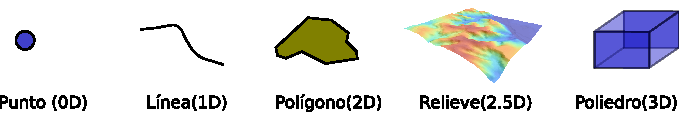
\includegraphics[width=.95\textwidth]{Introduccion_datos/Dimensiones.pdf}
\caption{\small Dimensi�n de los datos geogr�ficos}
\label{Fig:Dimensiones} 
\end{figure}

Por ultimo, un aspecto importante de toda variable estudiada es su \emph{continuidad}.\index{Continuidad} Se entiende esta continuidad como la capacidad de la variable para tomar todos los valores dentro de un rango definido. La temperatura, la presi�n o la elevaci�n son valores continuos, mientras que ninguna variable de tipo nominal puede ser continua, ya que se encuentra limitada a un numero (finito) de identificadores posibles. Por ejemplo, en el caso del n�mero de un DNI, los valores son siempre enteros, existe el valor 1 y el valor 2, pero no los infinitos valores decimales entre ambos.

La continuidad de la variable tem�tica se puede estudiar igualmente en relaci�n con la componente espacial. As�, existen variables que var�an de forma continua en el espacio, mientras que otras no lo hacen. Se emplea aqu� el concepto matem�tico de continuidad, es decir, que si traz�ramos un perfil de la variable a lo largo de un recorrido dado, la representaci�n de dicho perfil ser�a una curva que podr�a dibujarse sin levantar el l�piz del papel\footnote{Definiciones m�s rigurosas del concepto de continuidad puede encontrarse en cualquier texto b�sico de c�lculo elemental o, por ejemplo, en \cite{wikipediaContinuidad}}

Todas estas ideas referidas a las distintas variables (distintas informaciones que pretendemos recoger de una zona de estudio dada) nos servir�n para detallar los diferentes enfoques de representaci�n y almacenamiento que veremos en el pr�ximo cap�tulo, y escoger en cada caso el m�s apropiado.

\section{Divisi�n horizontal de la informaci�n geogr�fica}\label{divisionHorizontal}

Adem�s de dividir la informaci�n geogr�fica en componentes, tambi�n dividimos esta con criterios puramente espaciales, <<cort�ndola>> en unidades menores que ocupen una regi�n de amplitud m�s reducida. Este es un procedimiento similar al que encontramos en un mapa impreso, ya que el territorio de un pa�s se encuentra cartografiado en diferentes \emph{hojas}. Las razones para esto son, por una parte, los posibles distintos or�genes que los diferentes mapas pueden tener (cada regi�n puede ser responsable de fabricar los suyos) y, especialmente, el hecho de que, de no ser as�, los mapas tendr�an un tama�o inmanejable. Si cartograf�amos a escala\index{Escala} 1:25000 todo un pa�s, es obvio que no podemos hacerlo en un �nico mapa, ya que este ser�a enorme.

En el caso de trabajar en un SIG, no tenemos el problema del tama�o f�sico del mapa, ya que no existe tal tama�o. Los datos no ocupan un espacio f�sico, pero s� que requieren un volumen de almacenamiento, y este presenta el mismo problema. Recoger a escala 1:25000 todo un pa�s supone un volumen de datos enorme, que es conveniente dividir para poder manejar con fluidez.

En ambos casos, ya sea dentro de un SIG o no, suele resultar necesario emplear varios bloques de informaci�n (varias hojas) para cubrir un �rea de trabajo. En esta circunstancia, las propias caracter�sticas de un SIG y su forma de trabajo con los datos hacen que este proceso sea m�s sencillo y eficaz.

La principal cualidad de un SIG para integrar de forma transparente datos correspondientes a zonas distintas y formar un mosaico �nico es la separaci�n que existe entre datos y visualizaci�n. Los datos son la base de la visualizaci�n, pero en un SIG estos elementos conforman partes del sistema bien diferenciadas. Esto quiere decir que los datos se emplean para crear un resultado visual pero en s� mismos no contienen valores relativos a esa visualizaci�n.

De este modo, es posible combinar los datos y despu�s representarlos en su conjunto. Un proceso as� no puede realizarse con un mapa ya impreso, pues este contiene ya elementos de visualizaci�n e incluso componentes cartogr�ficos tales como una flecha indicando el Norte, una leyenda o una escala. Por ello, aunque puedan combinarse, realmente no se <<funde>> la informaci�n de cada uno de los mapas para conformar uno �nico. Dicho de otro modo, si tomamos cuatro hojas contiguas de una serie de mapas no podemos formar un nuevo mapa que sea indistinguible de uno cuatro veces m�s grande que haya sido impreso en un �nico pliego de papel. 

En un SIG, sin embargo, s� que sucede as�, y la visualizaci�n de cuatro o m�s bloques de datos puede ser id�ntica a la que obtendr�a si todos esos datos constituyeran un �nico bloque. Empleando herramientas habituales en un SIG, y si cada uno de esos bloques est� almacenado en un fichero, resulta incluso posible, unirlos todos y crear un solo fichero que los contenga.

Una de las razones principales que favorecen esta combinaci�n de datos es el hecho de que la escala nominal es en s� un elemento de representaci�n. Como vimos en el apartado \ref{Escala}, la escala nominal relaciona el tama�o que tiene un objeto en la representaci�n con su tama�o real, y la forma en que se recoge la informaci�n a la hora de realizar medidas de ese objeto viene condicionada por dicha escala, de tal modo que el esfuerzo desarrollado en esas mediciones sea coherente con la representaci�n que se va a hacer posteriormente al crear el mapa.

Los datos que manejamos en un SIG tiene una escala de detalle impuesta por la precisi�n de las mediciones, pero no una escala nominal asignada, ya que no tienen un tama�o fijo de representaci�n en la pantalla del ordenador o el perif�rico correspondiente, al contrario que un mapa impreso en el que los distintos elementos ya se encuentran representados. Esto hace que combinar cartograf�a cl�sica a distintas escalas sea complejo, ya que los mapas no <<casan>> bien entre s�.

En el caso de un SIG, es el usuario el que decide la escala de representaci�n, y esta ser� la misma para todos los datos que se visualicen, independientemente de las caracter�sticas de estos. En el contexto actual de datos geogr�ficos, es habitual encontrar situaciones en las que para una zona de terreno disponemos de informaci�n a una escala, y para otra zona contigua a esta la informaci�n disponible es a una escala distinta. Con el uso de un SIG, sin embargo, es posible trabajar sin problemas con todo el conjunto, sin preocuparse por la integraci�n de sus distintas partes.

L�gicamente, no debe dejarse de lado nunca el rigor cartogr�fico y, como se dijo en su momento, no olvidar que, aunque podamos representar cualquiera de esos datos a la escala que deseemos, los datos en s� no son suficientes para ello y tienen unas limitaciones impuestas por su escala inherente. Es decir, que no es  necesario preocuparse por la integraci�n a la ahora de visualizar y gestionar los datos, pero s� a la hora de analizarlos u obtener resultados a partir de ellos. No obstante, el proceso de combinaci�n es en cualquier caso transparente para el usuario que visualiza esos datos en un SIG, y la operaci�n pasa de ser algo tedioso y complejo a algo pr�cticamente inapreciable dentro del SIG, pues es este quien se encarga de ocultar toda esa complejidad y simplemente generar las representaciones seg�n los par�metros requeridos en cada momento.

\index{Uso conjunto de distintas escalas}
La figura \ref{Fig:Distintas_escalas_horizontal} muestra un ejemplo de lo anterior en el que puede verse c�mo varias fotograf�as a�reas forman un mosaico que cubre una zona dada, teniendo estas distinto nivel de detalle tal y como puede apreciarse.

\begin{figure}[!hbt] 
\centering
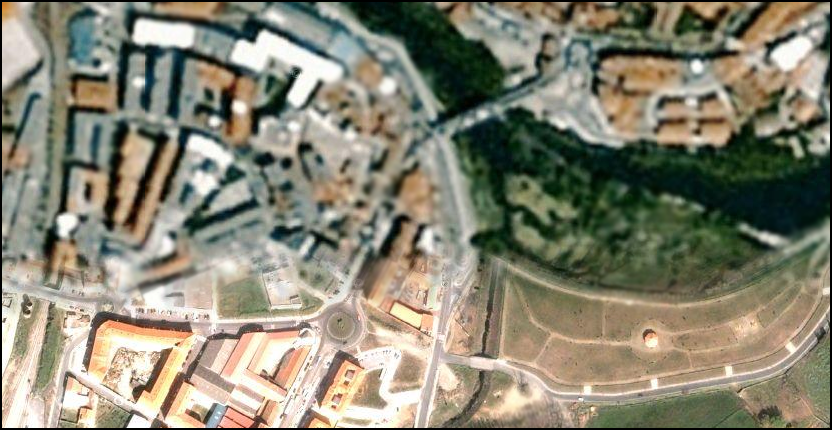
\includegraphics[width=.8\textwidth]{Introduccion_datos/Distintas_escalas_horizontal.png}
\caption{\small Integraci�n de datos en sentido horizontal. A pesar de que la escala de detalle es distinta para las fotograf�as a�reas de la imagen, estas se combinan sin problema en un SIG, represent�ndose a una escala dada todas ellas de forma sencilla. N�tese la mayor definici�n en la parte inferior de la imagen, que se forma con im�genes tomadas a una escala distinta a la de las de la parte superior. Advi�rtase igualmente la distinta iluminaci�n, ya que han sido tomadas en fecha y horas distintas.}
\label{Fig:Distintas_escalas_horizontal} 
\end{figure}


\section{Divisi�n vertical de la informaci�n. Capas}

Uno de los grandes �xitos de los SIG es su estructura de manejo de informaci�n geogr�fica, que facilita todas las operaciones que se llevan a cabo con esta. El concepto de \emph{capa}\index{Capa}, imprescindible para comprender todo SIG, es una de las grandes virtudes inherentes a los Sistemas de Informaci�n Geogr�fica, en cuanto que favorece la correcta estructuraci�n de la informaci�n y el trabajo con ella.

La divisi�n horizontal que ya hemos visto no es algo nuevo, y la gran mayor�a de los mapas cl�sicos cubren una porci�n relativamente peque�a de la superficie terrestre. Combinando distintos mapas podemos formar uno mayor que cubra una extensi�n m�s amplia, y aunque ya hemos visto que esto mismo puede realizarse con un SIG y la tarea resulta as� m�s sencilla, no resulta una operaci�n tan compleja y extra�a en el caso de no trabajar en un entorno SIG.

M�s dif�cil, sin embargo, es combinar distintos tipos de informaci�n, como por ejemplo la contenida en un mapa topogr�fico y la existente en un mapa de tipos de suelo y otro de vegetaci�n potencial. Para una misma zona, trabajaremos con varios mapas simultaneamente, y combinar estos para la realizaci�n de operaciones en las que intervengan todos ellos(supongamos, por ejemplo, calcular el �rea total de las zonas con un tipo de suelo dado donde la vegetaci�n corresponde a una clase concreta y se encuentran por encima de 1000 metros) es dif�cil y generalmente tambi�n impreciso.

En el caso de un SIG, los distintos tipos de informaci�n se pueden combinar de forma sencilla y limpia, y no aparecen los mismos problemas. Esto es as� debido a que la idea de capa permite dividir la informaci�n espacial referida a una zona de estudio en varios niveles, de tal forma que, pese a coincidir sobre un mismo emplazamiento, informaci�n sobre distintas variables se encuentra recogida de forma independiente. Es decir, en funci�n de la componente tem�tica se establecen distintos bloques de datos espaciales.

Para comprender mejor el concepto de capa, pensemos en un mapa topogr�fico cl�sico. En �l vamos a encontrar elementos como curvas de nivel, carreteras, n�cleos urbanos, o simbolog�a relativa a edificios y puntos singulares (iglesias, monumentos, etc.)  Todos estos elementos en su conjunto componen el mapa, y aparecen en una misma hoja como una unidad coherente de informaci�n geogr�fica. No obstante, cada uno de los de estos grupos de informaci�n recogidos ---elevaciones, red viaria, n�cleos urbanos, puntos de inter�s arquitect�nico--- pueden recogerse de forma independiente, y combinarse al componer el mapa seg�n las necesidades del momento, o bien combinarse de modo distinto o emplearse individualmente (Figura \ref{Fig:Concepto_capa}).

\begin{figure}[!hbt] 
\centering
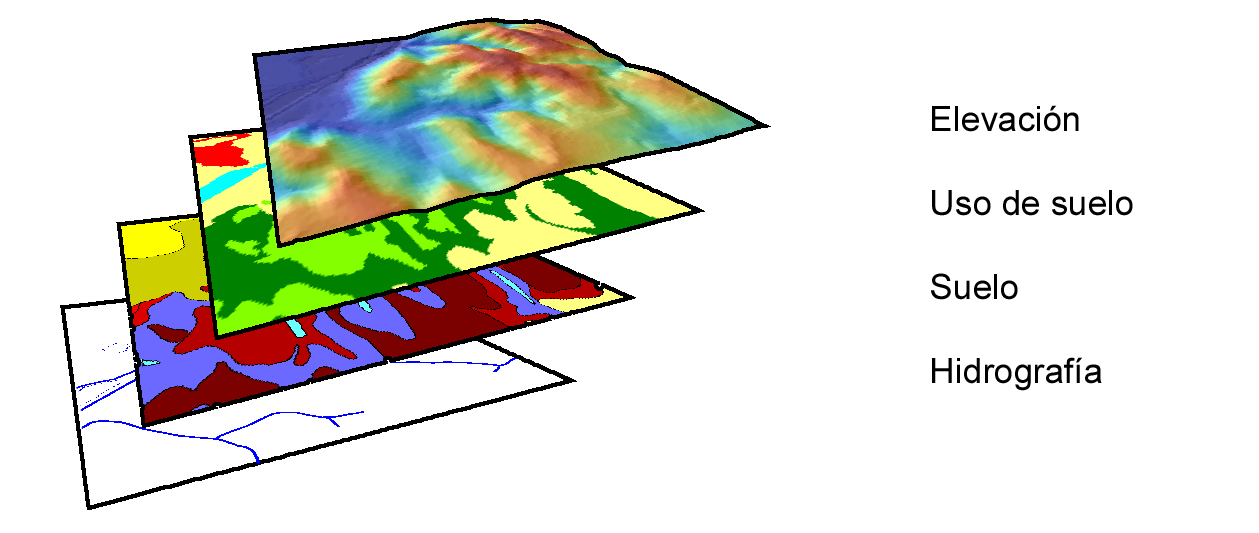
\includegraphics[width=.7\textwidth]{Introduccion_datos/Concepto_capa.png}
\caption{\small Concepto de \emph{capa} de informaci�n geogr�fica dentro de un SIG}
\label{Fig:Concepto_capa} 
\end{figure}

La figura es lo suficientemente gr�fica como para entender la raz�n de que a este tipo de divisi�n la denominemos \emph{vertical}, as� como el propio nombre de \emph{capa}, ya que de ella resulta una serie de diferentes niveles que se pueden superponer seg�n el criterio particular de cada usuario de SIG.

Toda la informaci�n geogr�fica con que trabajemos en un SIG va a ser en forma de capas. Sin ir m�s lejos, en el juego de datos de ejemplo que acompa�a a este libro se encontrar� la informaci�n dividida en capas, cada una de ellas haciendo referencia a un aspecto concreto de la zona recogida en dicho juego de datos. Cada una de estas capas puede abrirse de forma independiente en un SIG y utilizarse por s� misma o en conjunto con otras en la combinaci�n que se desee.\index{Datos!juego de}

Esta forma de proceder no es exclusiva de los SIG, y antes de la aparici�n de estos ya exist�an experiencias previas en este sentido, combin�ndose capas de informaci�n geogr�fica para la realizaci�n de an�lisis (v�ase \ref{Evolucion_tecnicas}). Es, sin embargo, con la aparici�n de los SIG cuando esta metodolog�a se aplica de forma regular y se establece sistem�ticamente dicha estructuraci�n de la informaci�n geogr�fica.

As�, la visualizaci�n, el an�lisis, y todas las acciones que se realizan sobre la informaci�n geogr�fica dentro de un SIG, se llevan a cabo sobre un conjunto de capas, entendi�ndose cada una de ellas como la unidad fundamental de informaci�n sobre una zona dada y un tipo de informaci�n concreta.

Muy habitualmente las capas se conocen tambi�n como \emph{capas tem�ticas} o \emph{temas}, t�rminos bastante extendidos que hacen referencia al mismo concepto.

La relevancia del concepto de capa como elemento fundamental de un SIG es enorme, pues realmente constituye el marco b�sico sobre el que se van a llevar a cabo gran parte de las operaciones. Algunas de las posibilidades que brinda esta filosof�a ya las conocemos. Por ejemplo, vimos en el apartado dedicado a la generalizaci�n cartogr�fica c�mo en un SIG podemos utilizar diferentes <<versiones>> de los datos correspondientes a una zona concreta, y representar una u otra de ellas en funci�n de la escala de trabajo. Para un tipo de informaci�n, por ejemplo los usos del suelo, estas versiones se almacenar�n como distintas capas.  La capa es as� la unidad fundamental no solo en t�rminos de un �rea dada, sino tambi�n de una escala concreta, y permite una divisi�n de los datos �ptima a todos los efectos.

Al igual que ve�amos en el apartado anterior, las capas nos van a permitir la combinaci�n de datos a distinta escala, no ya en este caso datos contiguos, sino datos correspondientes a un mismo �rea pero con variables distintas. Esto es de gran utilidad en el trabajo habitual, ya que no todas las variables se recogen con un mismo nivel de detalle, y el detalle con el que podemos encontrar una capa de elevaciones va a ser generalmente mucho mayor que el que cabe esperar para una capa de, digamos, litolog�a.

En realidad, y en el lenguaje habitual de trabajo con SIG, la capa no define �nicamente una divisi�n vertical, sino tambi�n una horizontal. Es m�s sencillo visualizar la idea de capa con un esquema como el de la figura \ref{Fig:Concepto_capa}, en el que las distintas variables se <<apilan>> en capas de informaci�n superpuestas. Sin embargo, las divisiones horizontales en un mosaico de datos tambi�n se consideran como capas distintas en un SIG, pese a contener una misma variable y un mismo tipo de informaci�n. Por tanto, y aunque la divisi�n vertical sea la que verdaderamente define la idea de capa, cuando hablamos de una capa de datos en un SIG nos referimos a un <<trozo>> de toda la informaci�n disponible, que implica una secci�n en la dimensi�n vertical (la de las variables existentes que pueden estudiarse) y un recorte en la horizontal (la de la superficie geogr�fica).

Las capas pueden emplearse tambi�n para incorporar en cierta forma la variable temporal si se considera que la dimensi�n vertical es el tiempo. Aunque no es la manera m�s adecuada, y en la actualidad el manejo del tiempo es uno de los principales problemas a resolver en el dise�o de los SIG, podemos trabajar con varias capas que representen una misma informaci�n y una misma zona, pero en instantes distintos. Esto no es distinto a trabajar con mapas cl�sicos correspondientes a diferentes instantes, salvo que en el caso de capas cada elemento de la informaci�n se encuentra separado a su vez.

Por �ltimo, es importante el hecho de que la separaci�n de la informaci�n en capas evita la redundancia de datos, ya que cada capa contiene un tipo de informaci�n concreto. En un mapa cl�sico se presentan siempre varias variables, algunas de ellas presentes con car�cter general, tales como nombres de ciudades principales o v�as m�s importantes de comunicaci�n. Es decir, que un mapa de usos de suelo o un mapa geol�gico van a contener otras variables, que en ocasiones se a�aden a este para enriquecerlo. Unas curvas de nivel, por ejemplo, permitir�n una mejor interpretaci�n de esa geolog�a.

Al dividir toda la informaci�n en capas, podemos combinar curvas de nivel y geolog�a, a�adir otros elementos, o bien representarlas de forma aislada, algo que no resulta posible si los datos de los que disponemos ya vienen unidos inseparablemente, como sucede en el caso de la cartograf�a impresa. La divisi�n en capas ofrece un mayor n�mero de posibilidades distintas de trabajo y, como iremos viendo a lo largo de gran parte de este libro, tambi�n mayores posibilidades de an�lisis y proceso.

En resumen, el trabajo con capas permite una estructura m�s organizada y una mayor atomizaci�n de los datos, con las consecuentes ventajas en el almacenamiento, manejo y funcionalidad que esto conlleva.


\section{Resumen}


Los datos son una de las piezas m�s importantes del sistema SIG. Entendemos por dato un conjunto de valores o elementos que representan algo. La interpretaci�n correcta de esos datos los dota de significado y produce \emph{informaci�n}.

La informaci�n geogr�fica tiene dos componentes: una componente tem�tica y una componente geogr�fica. Estas van unidas y conforman una unidad �nica de informaci�n geogr�fica, aunque pueden separarse y analizarse por separado. Mientras que la componente geogr�fica tiene un car�cter fundamentalmente num�rico, la componente tem�tica puede incluir una o varias variables y estas ser de naturaleza muy variada.

La informaci�n geogr�fica se divide horizontal y verticalmente. Las unidades mediante que incorporamos esta informaci�n a un SIG se conocen como \emph{capas}, y son uno de los elementos primordiales en la estructura de manejo de datos de todo SIG. El trabajo con capas m�s hace transparente la gesti�n de la informaci�n geogr�fica en un SIG, permite una mejor integraci�n de distintos datos, y es la base para muchas operaciones, algunas de las cuales iremos viendo en cap�tulos sucesivos.

%\bibliographystyle{unsrt}
%\bibliography{../../Libro_SIG}
\chapter{Modelos para la informaci�n geogr�fica}\label{Tipos_datos}

\begin{keypoints}
�Qu� pasos implica convertir la realidad geogr�fica en un modelo apto para su utilizaci�n en un SIG?$\bullet$�C�mo puede interpretarse y entenderse una realidad geogr�fica concreta de cara a su almacenamiento y an�lisis en un SIG?$\bullet$�Qu� es un modelo de representaci�n?$\bullet$�Por qu� son necesarios los modelos de representaci�n?$\bullet$�Cu�l es la relaci�n entre los modelos geogr�ficos conceptuales y los modelos de representaci�n de la informaci�n geogr�fica?$\bullet$�En qu� se basa el modelo de representaci�n r�ster y en qu� casos resulta m�s apropiado?�Y el modelo vectorial?
\end{keypoints} 

\bigskip

\begin{intro}
La realidad geogr�fica debe recogerse en un formato que pueda ser entendido por el ordenador y as� susceptible de emplearse dentro de un SIG. En este cap�tulo se mostrar�n los enfoques conceptuales y pr�cticos m�s frecuentes para llevar esto a cabo, que a su vez son los responsables indirectos de las arquitecturas subyacentes en los SIG. Para ello, se estudiar�n los distintos tipos de informaci�n con los que trabajamos en un SIG y las formas m�s adecuadas de entender, interpretar y manejar esta.
\end{intro}

\section{Introducci�n}

Los datos son, como ya sabemos, una parte imprescindible del SIG, ya que sin ellos, las aplicaciones SIG y los restantes elementos que se encuentran en torno a estas no tienen utilidad alguna. Necesitamos conocer el �rea geogr�fica que estudiamos en un SIG (es decir, tener datos sobre ella), para as� poder proceder a dicho estudio. 

No obstante, convertir ese �rea geogr�fica y la informaci�n acerca de ella en un dato susceptible de ser incorporado a un SIG no resulta una tarea sencilla. Desde los or�genes de los SIG, una de las preocupaciones principales ha sido la de representar de la mejor manera posible toda la informaci�n que podemos extraer de una zona geogr�fica dada, de tal modo que pueda almacenarse y analizarse en el entorno de un SIG. Este proceso de representaci�n, que ya desde el inicio planteaba problemas a los creadores de los primeros SIG, ha sido el responsable en gran medida de la arquitectura y forma de los SIG actuales, y a �l se debe en buena parte el desarrollo que han experimentado tanto los SIG en s� como las disciplinas afines.

Describir los enfoques te�ricos existentes para convertir la realidad relativa a una variable dada en una capa que la contenga de la forma m�s precisa posible y pueda ser empleada en un SIG es el objeto de este cap�tulo. Este proceso implica la construcci�n de un modelo (el dato geogr�fico), que representa la realidad y puede servir para conocer esta en profundidad a trav�s de an�lisis que no se llevan a cabo sobre dicha realidad, sino sobre el modelo en s�.

El problema principal reside en el hecho de que el detalle real que encontramos en la naturaleza es pr�cticamente infinito, mientras que la representaci�n y almacenamiento de esa realidad es finita. Se hace necesario extraer una serie de elementos y valores caracter�sticos, los cuales en ultima instancia se recoger�n como valores num�ricos dentro del SIG (pues son estos los que maneja un ordenador), y podr�n interpretarse como el anteriormente citado modelo. El camino que lleva desde la realidad hasta ese conjunto de meros valores num�ricos pasa por tres niveles:

\begin{itemize}
 \item Establecimiento de un modelo geogr�fico. Es decir, un modelo conceptual de la realidad geogr�fica y su comportamiento.
\item Establecimiento de un modelo de representaci�n. Es decir, una forma de recoger el anterior modelo conceptual y sus caracter�sticas propias, reduci�ndolo a una serie finita de elementos.
\item Establecimiento de un modelo de almacenamiento. Es decir, un esquema de c�mo almacenar los distintos elementos del modelo de representaci�n.
\end{itemize}
\index{Modelo!geogr�fico}\index{Modelo!de representacion}\index{Modelo!de almacenamiento}
El modelo geogr�fico es un ente puramente conceptual (de alto nivel), mientras que el de almacenamiento es m�s un concepto t�cnico inherente a la naturaleza inform�tica del SIG (de bajo nivel)

\section{Modelos geogr�ficos}

El primer paso hacia la creaci�n del dato geogr�fico implica el establecimiento de un modelo conceptual relativo a c�mo se ha de interpretar la realidad geogr�fica. Se trata de conceptualizar el espacio estudiado, la variable tratada y la variaci�n de esta a lo largo del espacio. Este modelo geogr�fico es un esquema mental que constituye una forma particular de entender el hecho geogr�fico en s�, pero que todav�a no incorpora elementos relativos a su representaci�n o almacenamiento.

Existen muchos modelos geogr�ficos distintos, entre los cuales cabe destacar dos de ellos \cite{Couclelis1992Springer}:

\begin{itemize}
 \item Campos
\item Entidades discretas
\end{itemize}

\index{Campos (modelo geogr�fico)}\index{Entidades!discretas}
\subsection{Campos}

Un campo es un modelo de variaci�n dentro de un marco n--dimensional, en el cual en cada punto dentro de dicho marco se tiene un valor de la variable estudiada. En su concepto matem�tico, un campo es una funci�n de la forma $\varphi:\mathbf{R}^n\rightarrow \mathbf{R}^m$, esto es, una funci�n que  asocia cada punto de un espacio vectorial con otro en un espacio vectorial distinto.

En el caso m�s habitual, $m=1$, es decir, que a cada punto del espacio vectorial origen se le asocia un �nico valor escalar. Se tiene as� lo que se denomina un \emph{campo escalar}. La mayor�a de las variables que se emplean en un SIG necesitan un �nico valor para describirse (pi�nsese en variables como la elevaci�n, la temperatura o la presi�n atmosf�rica, que solo requieren de un n�mero para expresarse), por lo que los campos escalares son los m�s habituales en el �mbito geogr�fico. 

\index{Campo!escalar}\index{Campos!vectorial} \index{Vectorial!campo}
No obstante, tambi�n encontramos los denominados \emph{campos vectoriales}\footnote{El empleo del t�rmino \emph{vectorial} para calificar a los campos vectoriales o los espacios vectoriales no debe confundirse con el modelo de representaci�n vectorial que veremos m�s adelante en este cap�tulo. En el caso de campos y espacio, se trata de la terminolog�a est�ndar del �mbito matem�tico, mientras que en el modelo de representaci�n vectorial es una terminolog�a propia de los Sistemas de Informaci�n Geogr�fica.}, en el cual el espacio vectorial de destino es multidimensional. Por ejemplo, para definir el movimiento del viento en un punto geogr�fico no basta con un �nico valor, sino dos: la velocidad y la direcci�n en la que sopla dicho viento. Dentro de un SIG, es habitual recoger los campos vectoriales como un conjunto de varios campos escalares, cada uno de ellos en una capa distinta. As�, se tendr�a una capa con la direcci�n y otra con la velocidad, ambas magnitudes escalares. Operando de esta manera, la soluci�n no es �nica, ya que el vector resultante puede definirse mediante su m�dulo y direcci�n (como en el caso anterior), pero tambi�n por sus propias coordenadas en la base del espacio vectorial destino (en el caso anterior, las componentes $x$ e $y$ del vector que indica el movimiento del viento).

\index{Espacio!vectorial}\index{Vectorial!espacio}

El espacio vectorial de origen puede ser bidimensional, es decir, una funci�n de la forma $f(x,y)$, representando $x$ e $y$ las coordenadas geogr�ficas. Este es el caso habitual en las capas que se emplean en un SIG, donde las variables que estudiamos adquieren uno u otro valor en funci�n de su posici�n dentro de un sistema coordenado de referencia.

Puede a�adirse una tercera dimensi�n, de tal modo que los valores dependan no solo de la posici�n sino igualmente de la elevaci�n. Se tendr�a una funci�n de la forma $f(x,y,z)$. Para el caso, por ejemplo, de la temperatura del aire, esta depende no solo de la localizaci�n, sino tambi�n de la altura. Otro ejemplo puede ser el porcentaje de arena en el suelo, que depende de la localizaci�n pero tambi�n de la profundidad.

Igualmente, aunque en general es poco habitual en el marco de los SIG, puede a�adirse la variable tiempo, teni�ndose funciones de la forma $f(x,y,t)$ o $f(x,y,z,t)$\index{Tiempo}

Por definici�n, un campo es continuo\index{Continuidad}, ya que todos los puntos tienen un valor asociado. De igual modo, este valor es �nico, y no existe un elemento del espacio vectorial de partida que tenga asociados varios elementos del de destino, sean estos escalares o vectores.

Por su propia naturaleza los campos son ideales para modelizar variables que var�an de forma continua en el espacio, entre ellas la practica totalidad de variables f�sicas del medio, tales como temperatura del aire, presi�n atmosf�rica, elevaci�n, etc.

Los campos se asocian con las denominadas \emph{coberturas}, termino este m�s empleado en el �mbito SIG. En una cobertura existe un valor �nico para todos los puntos de una regi�n dada.\index{Cobertura}

\subsection{Entidades discretas}

A diferencia de los campos, el modelo de entidades discretas no asocia a cada punto geogr�fico un valor, sino que concibe un entorno geogr�fico como un espacio vac�o sobre el que se sit�an distintos elementos (entidades) que lo van rellenando. Cada una de dichas entidades posee unas caracter�sticas propias, constantes para toda ellas, que son las que conferir�n sus propiedades particulares a los puntos que se sit�en en su interior.

Un punto puede no pertenecer a ninguna entidad, o bien a varias de ellas, seg�n sea la disposici�n de estas. Para un espacio dado, las entidades pueden ser todos aquellos elementos geom�tricos existentes en el mismo, tales como puntos, l�neas, pol�gonos o, en el caso de ser dicho espacio de dimensi�n mayor que dos, tambi�n vol�menes.

Es f�cil ver que el modelo de entidades discretas no es tan adecuado como los campos para conceptualizar variables continuas, ya que la continuidad de estas es opuesta al esquema discreto planteado. No obstante, otras variables no continuas se modelizan mejor mediante entidades discretas, ya que la forma en que se presentan coincide en cierta medida con dichas entidades como unidades m�nimas. 

La presencia de v�as de comunicaci�n, por ejemplo, se puede asimilar perfectamente a este modelo. Se tiene un espacio vac�o (sin v�as), en el cual se disponen los distintos viales en una serie de localizaciones concretas. Hay puntos que no estar�n afectados por ninguna entidad, mientras que otros (los situados en las intersecciones) lo est�n por varias de ellas.

Las variables de tipo nominal y alfanum�rico ---las cuales no son, como vimos, continuas---tales como el tipo de suelo en un punto o el n�mero de parcela catastral al que pertenece dicho punto, tambi�n se adaptan bien al modelo de entidades discretas.
\index{Nominal}

Otra diferencia entre los campos y las entidades discretas es que estas �ltimas son en general m�s sencillas de comprender como concepto fuera de un �mbito t�cnico. Los campos son conceptos matem�ticos que requieren un mayor grado de abstracci�n, y para la mayor�a de la gente no resultan tan claros. Como algunos apuntan \cite{NCGIA}, el lenguaje habitual contiene un numero mayor de expresiones y recursos para describir la realidad geogr�fica en base a entidades discretas que en base a campos o conceptos abstractos similares.

\section{Modelos de representaci�n}

Los modelos geogr�ficos nos ofrecen una concepci�n particular del espacio geogr�fico y sus atributos. En base a ellos, el siguiente paso es reducir las propiedades de dichos modelos a un conjunto finito de elementos, de tal modo que el registro de dichos elementos sirva para almacenar la realidad que los modelos geogr�ficos describen. Para ello, empleamos los \emph{modelos de representaci�n}, tambi�n denominados \emph{modelos de datos}.

\index{Modelos!de datos}\index{Modelos!de representacion}\index{Datos!modelos de}

Antes de entrar a describir los distintos modelos de representaci�n, veamos algunos ejemplos que nos presentar�n casos particulares de estos modelos, aclarando sus diferencias antes de proceder a una definici�n m�s detallada. En la figura \ref{Fig:MDE_modelos_representacion} pueden verse distintas formas de representar la elevaci�n de una zona, la cual, como ya sabemos, es una variable continua y puede concebirse mediante un campo escalar. Por el contrario, la red viaria se adapta mejor a un modelo de entidades discretas, y se muestran en la figura \ref{Fig:Vias_modelos_representacion} sendas representaciones de esta variable seg�n distintos modelos de datos. Mediante los ejemplos de estas figuras presentaremos los modelos de datos principales, as� como su relaci�n con los modelos conceptuales estudiados en el punto anterior.

\index{Modelo Digital de Elevaciones}

\begin{figure}[!hbt]   
\centering
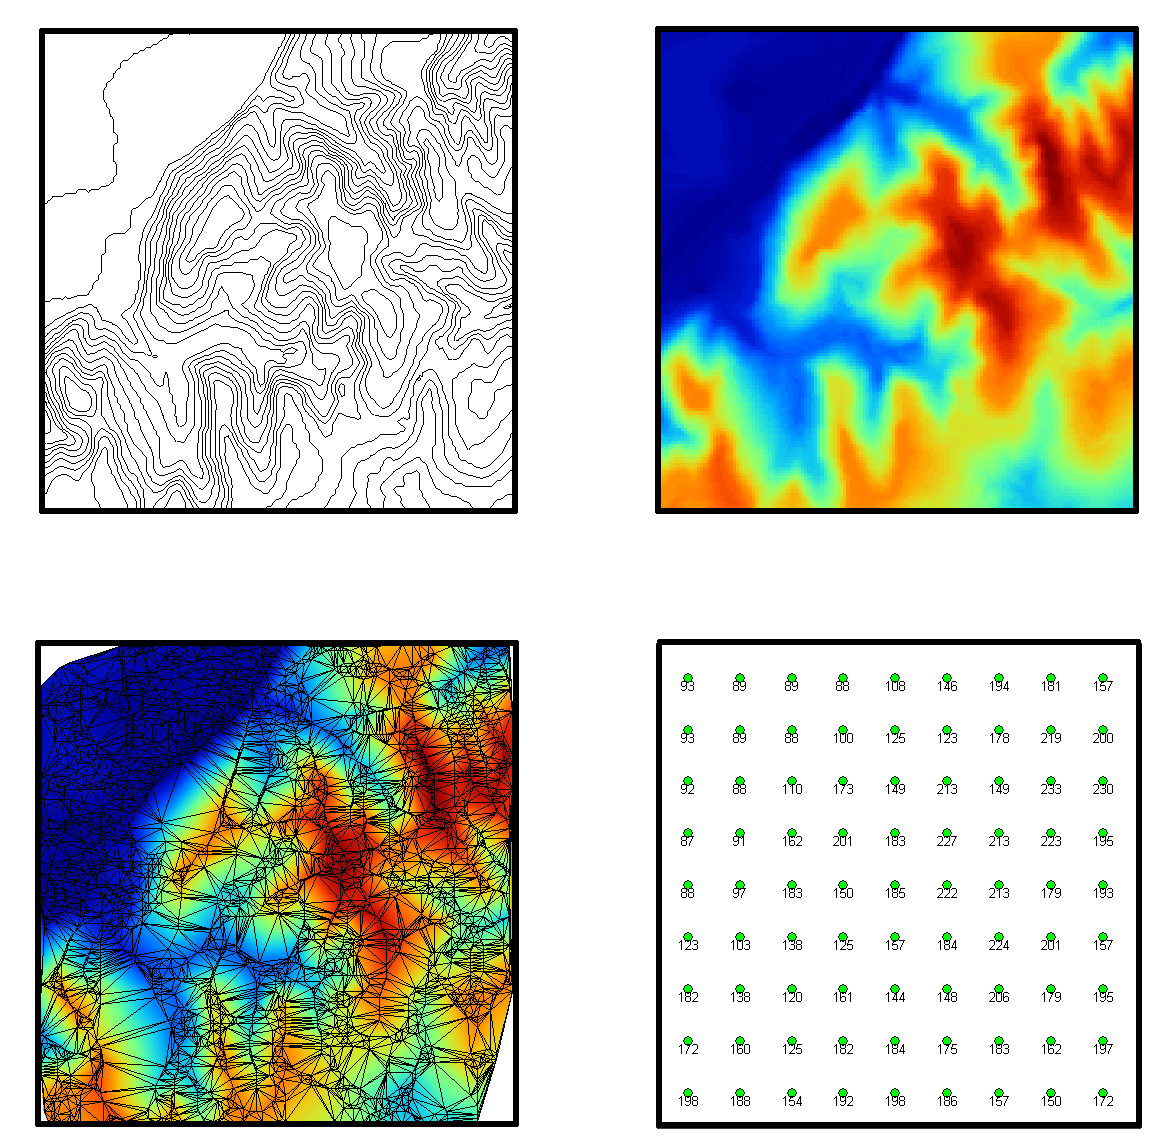
\includegraphics[width=.7\textwidth]{Tipos_datos/MDE_modelos_representacion.png}
\caption{\small Distintas formas de representar una capa con informaci�n altitudinal.}
\label{Fig:MDE_modelos_representacion} 
\end{figure}

\begin{figure}[!hbt]   
\centering
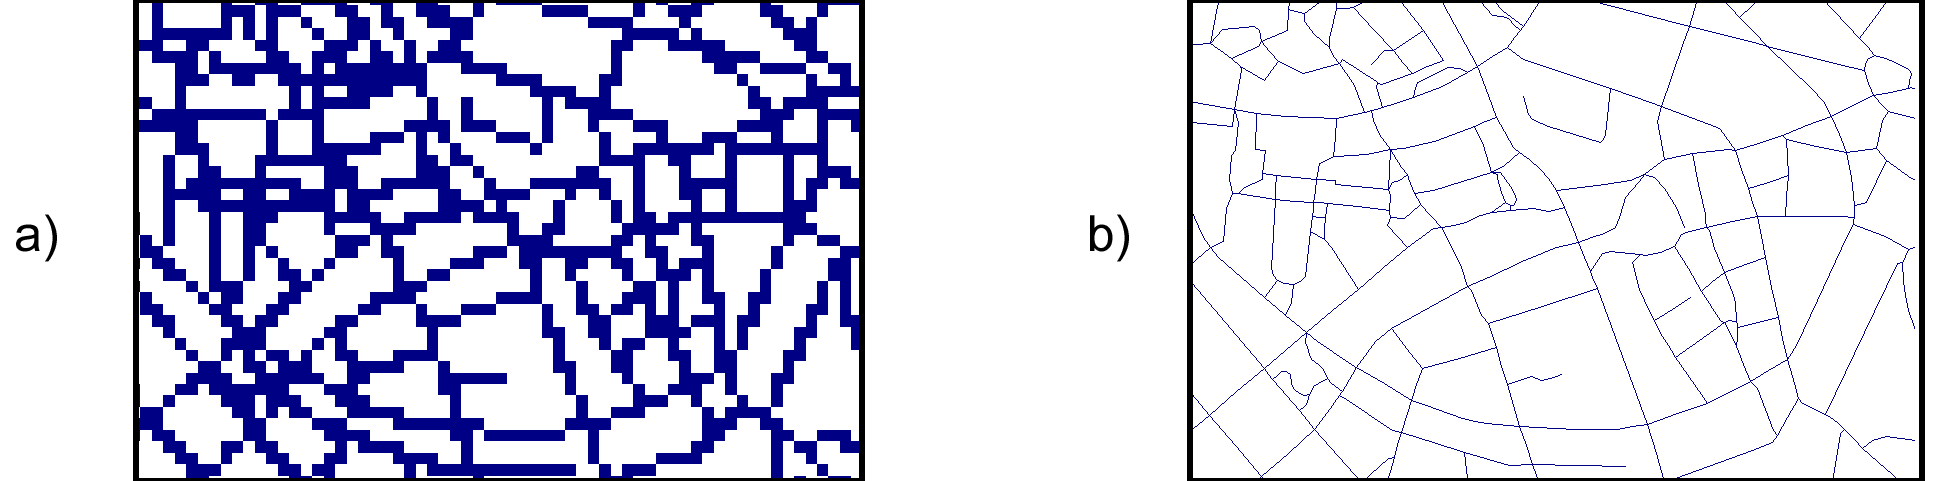
\includegraphics[width=.9\textwidth]{Tipos_datos/Vias_modelos_representacion.png}
\caption{\small Distintas formas de representar una capa con informaci�n sobre una red viaria.}
\label{Fig:Vias_modelos_representacion} 
\end{figure}

Comenzando con la elevaci�n, encontramos cuatro distintas formas de representarla, a saber:

\begin{itemize}
 \item Curvas de nivel. La representaci�n cl�sica empleada tradicionalmente en los mapas de papel. Se recoge la elevaci�n en una serie de curvas, que marcan los puntos en los que dicha elevaci�n es m�ltiplo de una cierta cantidad (la equidistancia). En el ejemplo propuesto, se muestran curvas con elevaciones m�ltiplos de 10 metros.
\item Una malla de celdas regulares, en cada una de las cuales se dispone un valor, que corresponde a las caracter�sticas de la zona ocupada por dicha celda. En este caso, cada celda tiene un valor de altura propio, que al convertirse en un color mediante el uso de una escala de colores, da lugar a la imagen mostrada.
\item Puntos regulares. Una serie de puntos regularmente espaciados. Existe informaci�n de la elevaci�n solo en dichos puntos. La informaci�n se muestra como etiqueta asociada a cada punto.
\item Red de Tri�ngulos Irregulares. Una Red de Tri�ngulos Irregulares (TIN en sus siglas inglesas, de \emph{Triangulated Irregular Network}), es una estructura en la cual se toman los puntos m�s caracter�sticos del relieve y en base a ellos se construye una teselaci�n en tri�ngulos con unas condiciones particulares. Cada uno de los tri�ngulos posee unas propiedades comunes en cuanto a su relieve. Veremos m�s adelante en detalle este tipo de estructuras. Por el momento, basta recordar que los elementos b�sicos de esta forma de representaci�n son tri�ngulos.
\end{itemize}\index{Triangulated Irregular Network (TIN)}

Para el caso de las v�as encontramos dos representaciones distintas:

\begin{itemize}
 \item Una malla como la citada en el caso anterior. Las celdas de v�a tiene un valor (representado aqu� en azul) distinto de las que se encuentran fuera de la v�a (con valor representado aqu� en blanco)
\item Un conjunto de l�neas representando los trazados de las v�as.
\end{itemize}

En este ultimo caso las celdas se han elegido de un tama�o excesivamente grande, con el fin de que pueda apreciarse de forma inmediata la diferencia existente. Veremos m�s adelante que, como no es dif�cil intuir, la representaci�n mediante celdas no es tan adecuada para el caso de una capa de v�as (aunque para el caso de la elevaci�n da lugar a una imagen con un aspecto inmejorable y altamente informativo), cuando estudiemos los aspectos relativos a la precisi�n en los distintos modelos de almacenamiento. 

Como vemos, para un mismo tipo de informaci�n existen diversas alternativas en cuanto a la forma de materializar la realidad y plasmar el modelo geogr�fico concreto. Estas formas las podemos clasificar en dos grupos principales: modelo de representaci�n \emph{r�ster} y modelo de representaci�n \emph{vectorial}. 

\index{Raster!modelo}\index{Vectorial!modelo}

Si se han seguido los cap�tulos de partes anteriores, probablemente los t�rminos \emph{r�ster} y \emph{vectorial} no resulten extra�os, ya que han aparecido con cierta frecuencia. Esto es as� porque, adem�s de definir dichos t�rminos los principales modelos de representaci�n de la informaci�n geogr�fica dentro de un SIG, se han venido utilizando tradicionalmente para definir a los SIG en s�, en funci�n de si sus capacidades se hallaban m�s enfocadas al manejo y an�lisis de informaci�n en formato r�ster o en formato vectorial. A d�a de hoy, esa diferencia no es tan patente y los SIG m�s habituales pueden trabajar con ambos indistintamente, pudiendo realizar las tareas que resultan m�s adecuadas de llevar a cabo tanto con uno como con otro tipo de representaci�n. 

En lineas generales podemos decir que el modelo r�ster se basa en una divisi�n sistem�tica del espacio, la cual cubre todo este (a este concepto se le denomina se denomina \emph{teselaci�n}), caracteriz�ndolo como un conjunto de unidades elementales (las celdas de las mallas vistas en los ejemplos). El modelo vectorial, por su parte, no divide el espacio completamente, sino que lo define mediante una serie de elementos geom�tricos con valores asociados, siendo la disposici�n de estos no sistem�tica, sino guardando relaci�n con los objetos geogr�ficos presentes en la zona de estudio.

\index{Teselaci�n}

En un principio, puede pensarse que el modelo r�ster se asemeja al modelo geogr�fico de campos, mientras que el vectorial concuerda con el de entidades discretas. Aunque en cierta medida puede considerarse que as� sucede y existe tal dualidad, no es del todo cierta esta equiparaci�n, como discutiremos con algo m�s de detalle en los siguientes puntos.

De forma esquem�tica, los enfoques de los modelos de representaci�n r�ster y vectorial se muestran en la figura \ref{Fig:Esquemas_modelos_representacion}

\begin{figure}[!hbt]   
\centering
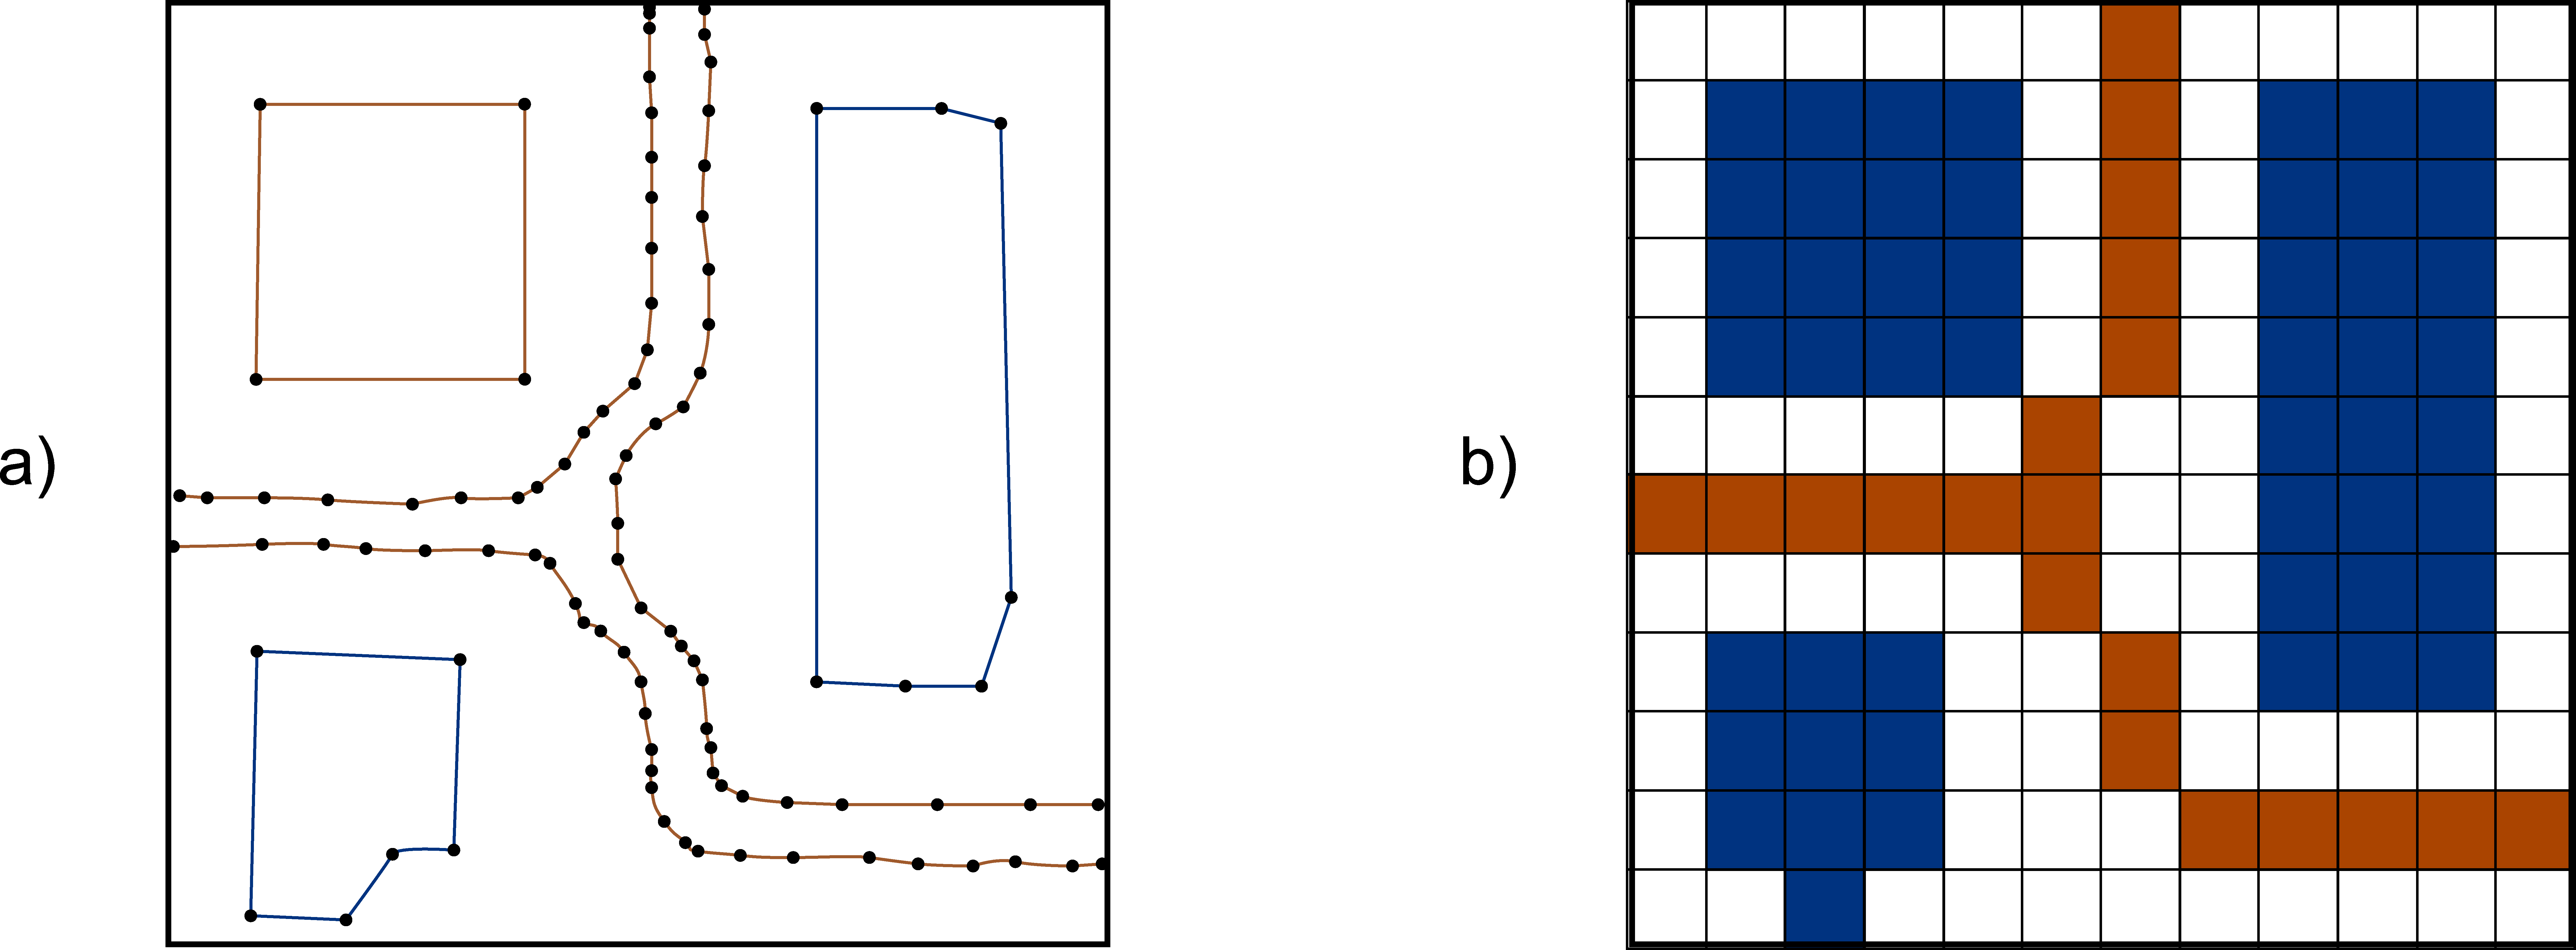
\includegraphics[width=.9\textwidth]{Tipos_datos/Esquemas_modelos_representacion.pdf}
\caption{\small Comparaci�n entre los esquema del modelo de representaci�n vectorial (a) y r�ster (b).}
\label{Fig:Esquemas_modelos_representacion} 
\end{figure}

Podemos entender estos enfoques haciendo uso del esquema de Sinton presentado con anterioridad. En el modelo vectorial controlamos la definici�n de los valores asociados, y medimos la localizaci�n y forma de estos, dejando fijo el tiempo. En el modelo r�ster, aunque la componente temporal tambi�n es fija, la componente que controlamos es la espacial (a trav�s de la sistematicidad de la malla), mientras que medimos la naturaleza de los valores en cada una de las celdas.

\index{Sinton!esquema de}

Antes de pasar a la definici�n detallada de los modelos r�ster y vectorial, mencionar que, como modelos principales empleados para la definici�n de capas de informaci�n geogr�fica, las expresiones \emph{capa vectorial} y \emph{capa r�ster} son de uso habitual, y se emplear�n de aqu� en adelante tanto en este como en posteriores cap�tulos.

\subsection{Modelo r�ster}\label{Modelo_raster}\index{Raster!modelo}

En el modelo r�ster, la zona de estudio se divide de forma sistem�tica en una serie de unidades m�nimas (denominadas habitualmente \emph{celdas}), y para cada una de estas se recoge la informaci�n pertinente que la describe.  Se puede ver esto en detalle en la figura \ref{Fig:Raster_closeup}, que muestra aumentada una porci�n la malla r�ster de elevaciones de la figura \ref{Fig:MDE_modelos_representacion}, de modo que los l�mites de las celdas se hacen patentes y puede adem�s representarse en cada una de ellas su valor asociado.

\begin{figure}[!hbt]   
\centering
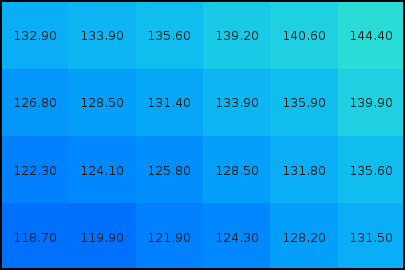
\includegraphics[width=.4\textwidth]{Tipos_datos/Raster_closeup.png}
\caption{\small Celdas de una malla r�ster con sus valores asociados.}
\label{Fig:Raster_closeup} 
\end{figure}

Aunque la malla de celdas puede contener informaci�n sobre varias variables, lo habitual es que trate una �nica variable. Es decir, que se tenga un �nico valor para cada una de las celdas.

La caracter�stica principal del modelo r�ster, y que le confiere gran parte de sus propiedades m�s interesantes, especialmente de cara al an�lisis, es su sistematicidad. La divisi�n del espacio en unidades m�nimas se lleva a cabo de forma sistem�tica de acuerdo con alg�n patr�n, de tal modo que existe una relaci�n impl�cita entre las celdas, ya que estas son contiguas entre s�, cubren todo el espacio, y no se solapan. Por tanto, la posici�n de una celda depende de la de las restantes, para as� conformar en conjunto toda la malla regular que cumple las anteriores caracter�sticas. Dicho de otro modo, el orden propio de las celdas, presente gracias a la divisi�n sistem�tica realizada, aporta un elemento adicional que las relaciona entre s�.

\index{Raster! de celdas no rectangulares}

Como unidad m�nima pueden tomarse elementos de diversas formas. La m�s habitual es mediante unidades de forma cuadrada, aunque tambi�n pueden ser formas rectangulares, o incluso triangulares o hexagonales \cite{Diaz1986Reading}. No obstante, los SIG habituales se limitan a modelos de celdas cuadradas, y las implementaciones de otros modelos son de uso muy reducido y en aplicaciones muy especificas que en general no est�n orientadas al uso general ni disponibles de forma accesible al usuario com�n. Junto a esto, la informaci�n geogr�fica en formatos r�ster distintos de la divisi�n en celdas cuadradas es pr�cticamente inexistente, haciendo m�s dif�cil el empleo de estos formatos en condiciones normales de trabajo.

De igual modo, existen representaciones r�ster no regulares, en las que todas las unidades m�nimas no tienen un mismo tama�o. Este tipo de representaciones no tiene apenas presencia en los SIG, pero son habituales en otros �mbitos tales como el de la representaciones 3D, con unos requerimientos bien distintos\footnote{V�ase, por ejemplo, el concepto de Nivel Continuo de Detalle (Continuous Level of Detail, CLOD), para lograr representaciones de detalle con el menor gasto de recursos posible, y que es habitual en este campo.}. Esto est� relacionado a su vez con los modelos de almacenamiento r�ster, que veremos m�s adelante en este mismo cap�tulo.

\index{Continuous Level of Detail (CLOD)}

En todos los casos, la divisi�n en celdas no depende de la variable estudiada, y es una divisi�n geogr�fica. Esto lo diferencia de otras divisiones como el caso de la Red de Tri�ngulos Irregulares, que, a pesar de ser una teselacion que cubre todo el espacio, est� basada en la propia variable de elevaci�n, y dicha divisi�n (n�mero, forma y disposici�n de los tri�ngulos) ser�a distinta en caso de que los valores de elevaci�n fueran otros.

\index{Triangulated Irregular Network (TIN)}

Siendo, pues, las mallas r�ster de celdas cuadradas las m�s habituales, pasemos a ver algo m�s acerca de estas y su elementos b�sicos. Dos son los elementos principales que resultan necesarios para una definici�n completa de una capa r�ster:

\begin{itemize}
\item Una localizaci�n geogr�fica exacta de alguna celda y una distancia entre celdas, para en base a ellas, y en virtud de la regularidad de la malla, conocer las coordenadas de las restantes.
\item Un conjunto de valores correspondientes a las celdas.
\end{itemize}

En el modelo r�ster no se recogen de forma expl�cita las coordenadas de cada una de las celdas, sino tan solo los valores de estas. No resulta necesario acompa�ar a dichos valores de un emplazamiento espacial concreto, pues hacen referencia a un elemento particular de la malla, la cual representa una estructura fija y regular. No obstante, s� que es necesario emplazar dicha malla en el espacio para despu�s poder calcular las coordenadas particulares de cada celda.

Lo m�s habitual es definir el emplazamiento de una �nica celda (habitualmente la celda superior izquierda), una orientaci�n fija, y una distancia entre las celdas (el paso de la malla). Como se muestra en la figura \ref{Fig:Elementos_capa_raster}, esto ya permite, mediante un sencillo c�lculo, conocer las coordenadas de todas las celdas sin necesidad de almacenar estas.

\begin{figure}[!hbt]   
\centering
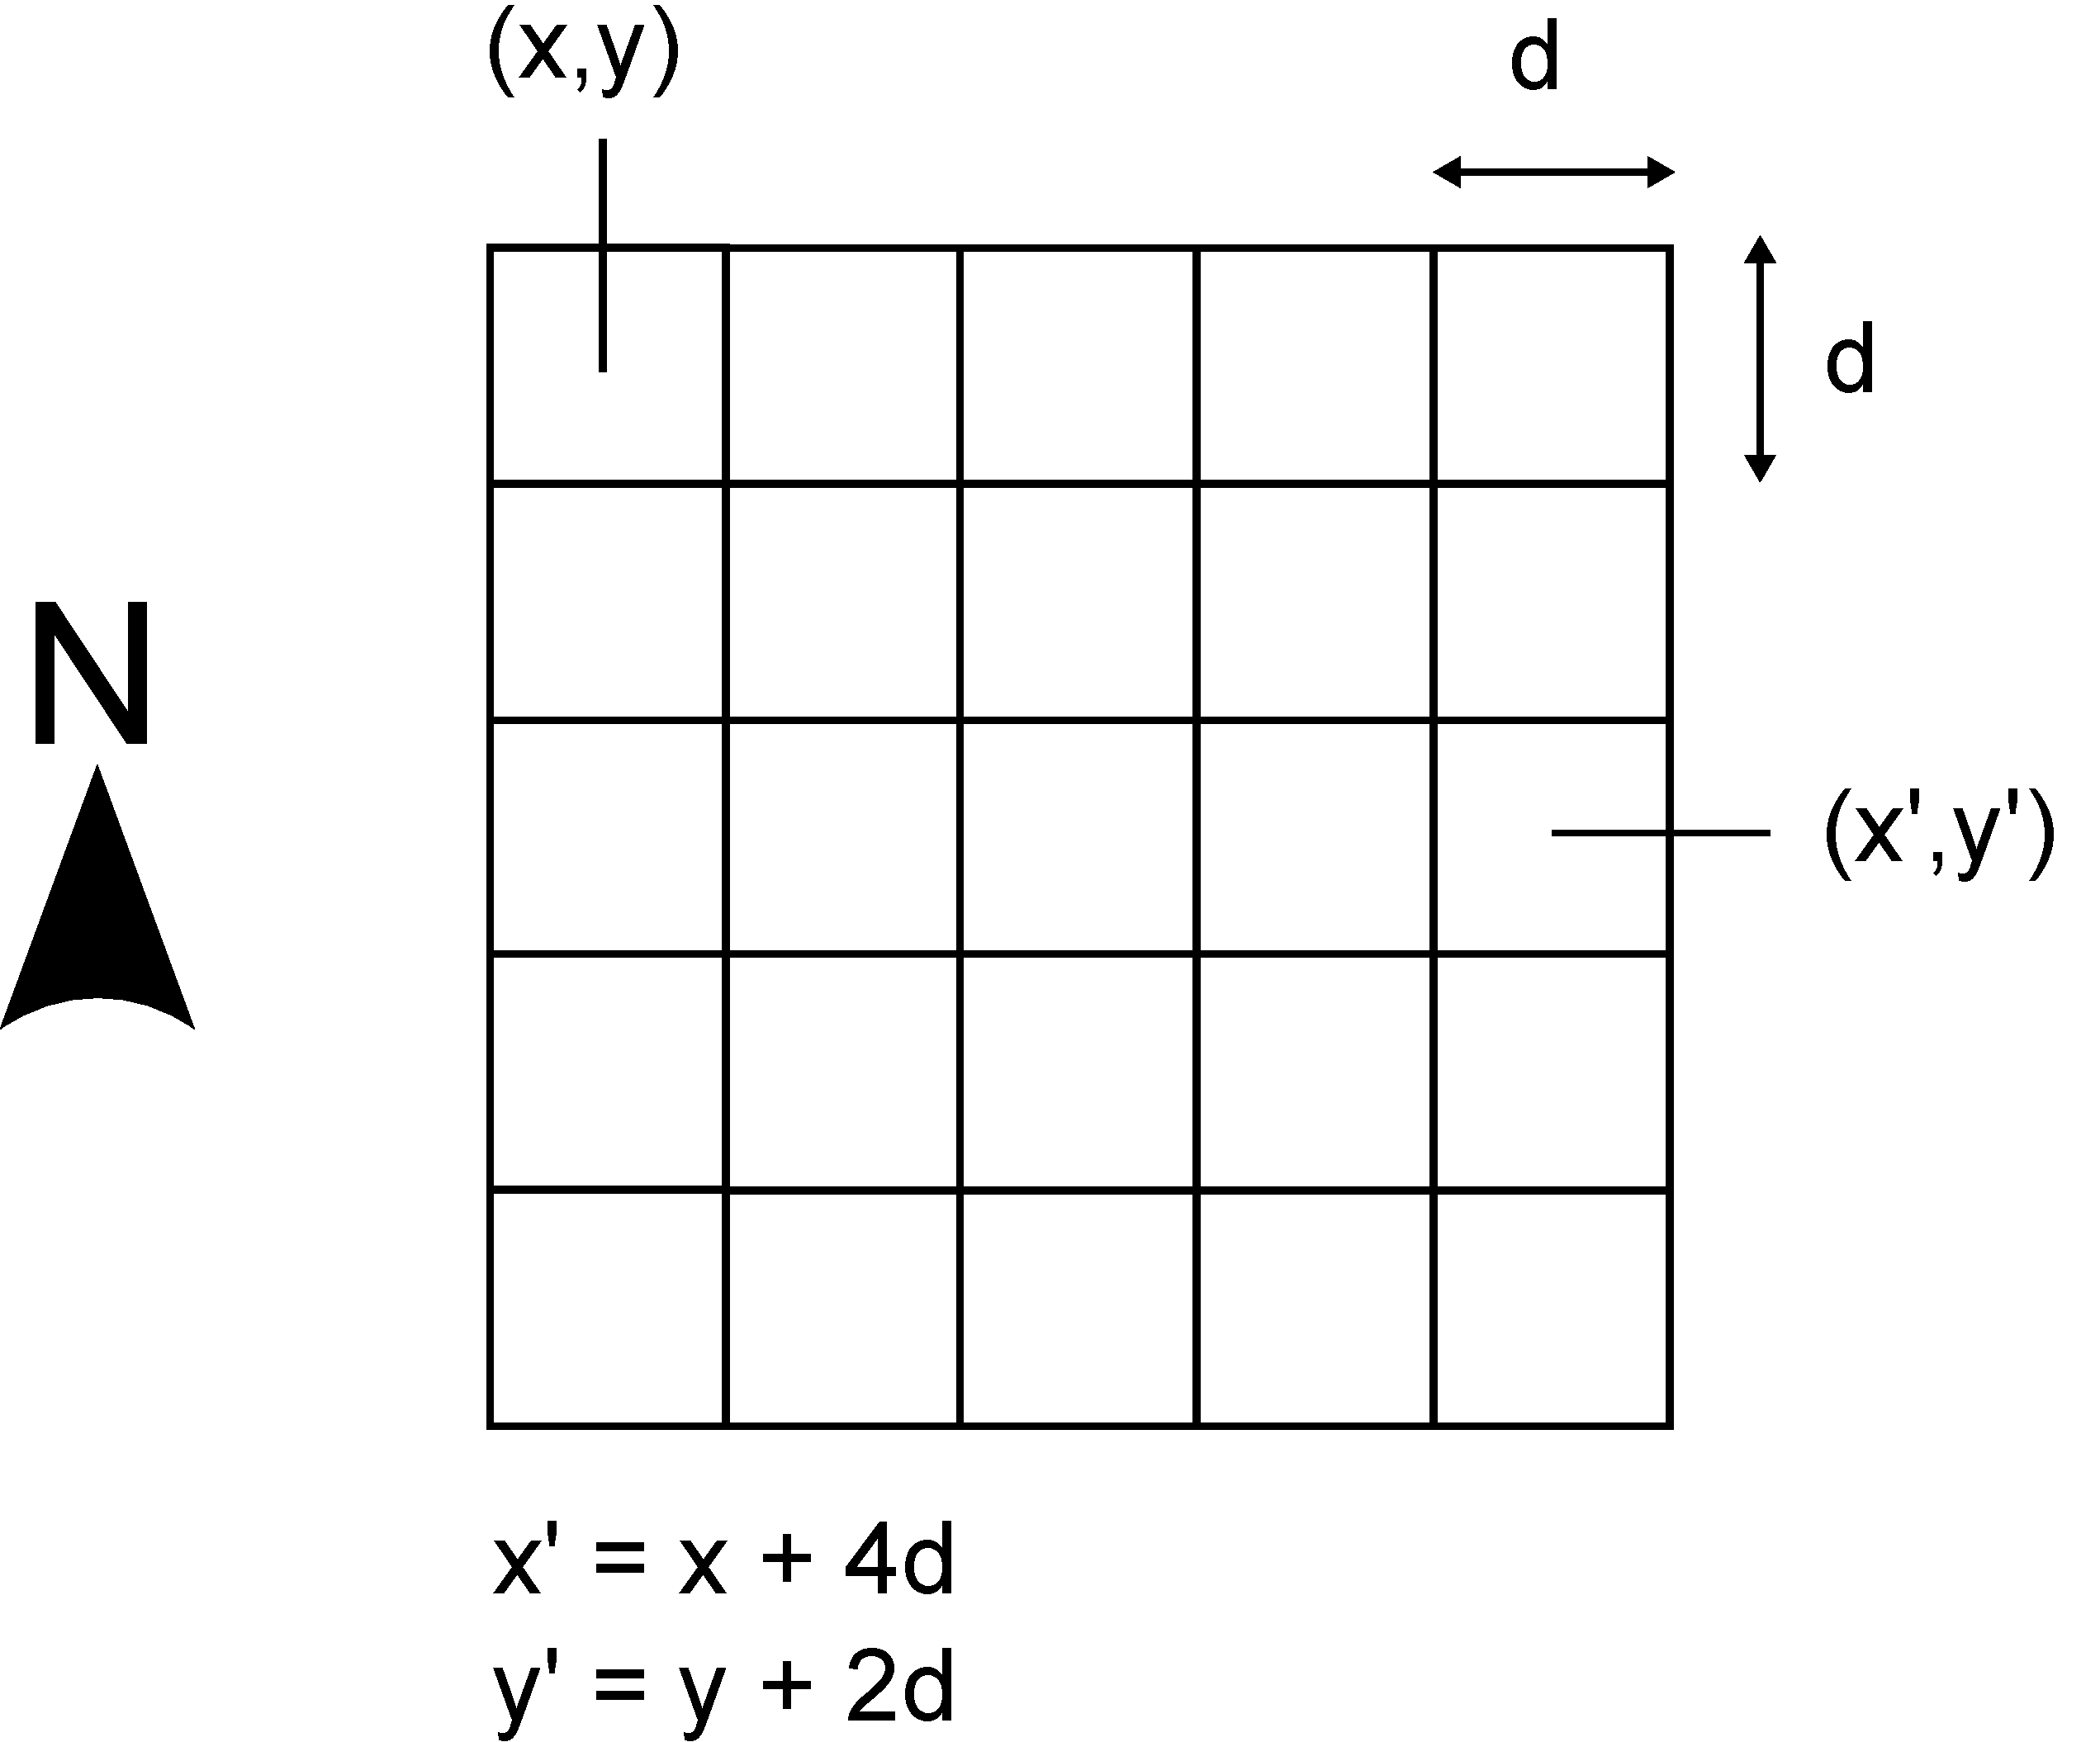
\includegraphics[width=.4\textwidth]{Tipos_datos/Elementos_capa_raster.pdf}
\caption{\small La estructura regular de la malla r�ster permite conocer las coordenadas de las celdas sin necesidad de almacenar estas, sino tan solo recogiendo algunos par�metros de la malla como la localizaci�n de una celda base ($x,y$), la orientaci�n global o el tama�o de celda ($d$).}
\label{Fig:Elementos_capa_raster} 
\end{figure}

La orientaci�n de las capas r�ster es habitualmente Norte--Sur, de tal modo que si pasamos de la primera a la segunda fila estamos descendiendo en latitud (este hecho ser�a matizable en funci�n de la proyecci�n empleada). Dicho de otra forma, la parte de arriba de la imagen es el norte, y la de abajo es el sur. Esta convenci�n simplifica el trabajo con capas r�ster dentro de un SIG y permite aplicar directamente la f�rmula mostrada en la figura \ref{Fig:Elementos_capa_raster}.

No obstante, puede suceder que la fuente de datos original no se adhiera a este formato (por ejemplo, una fotograf�a a�rea en la que el avi�n no volaba en direcci�n Norte--Sur o perpendicular, o una porci�n de un mapa escaneado que no tiene tampoco esa orientaci�n). En tal caso, y puesto que los SIG trabajan en general con tal orientaci�n en sus representaciones y a la hora de incorporar capas r�ster, nos encontraremos con situaciones como la mostrada en la figura \ref{Fig:Malla_raster_rotada}

\begin{figure}[!hbt]   
\centering
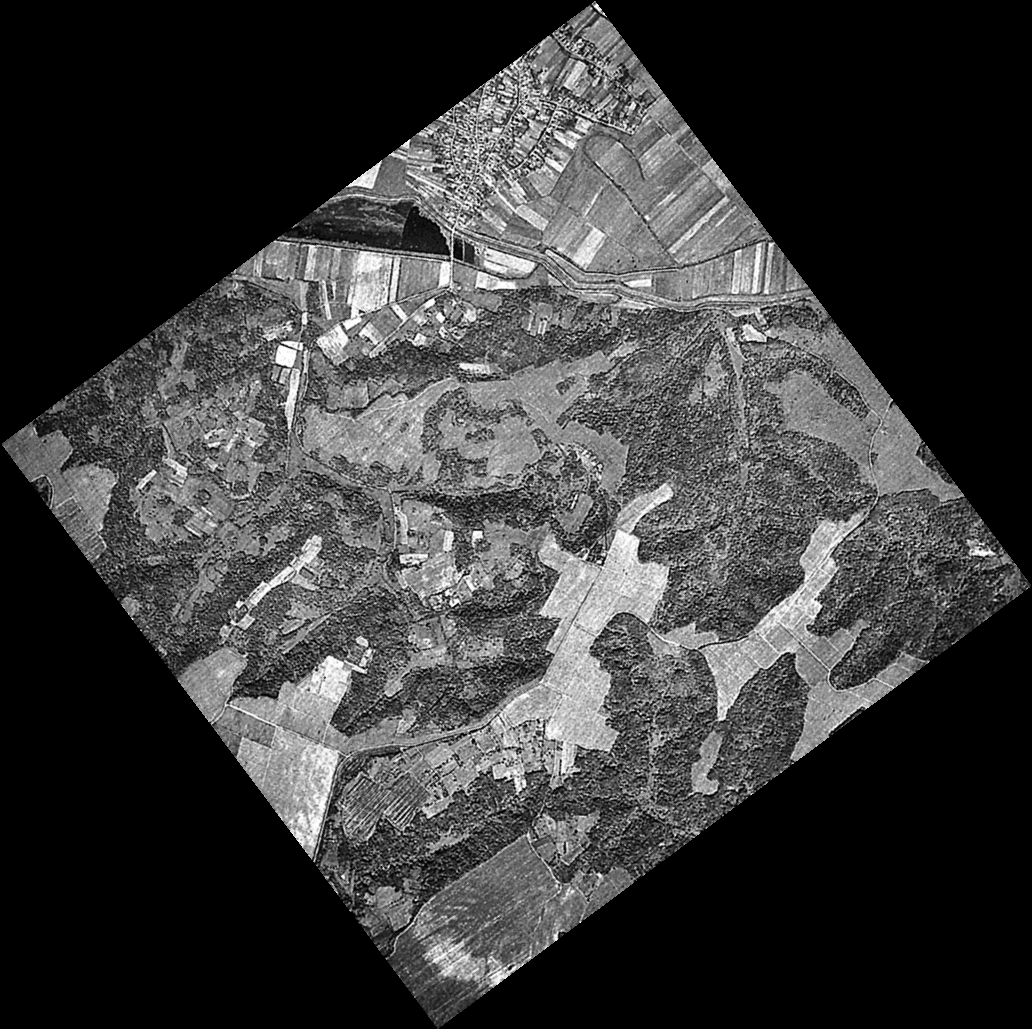
\includegraphics[width=.5\textwidth]{Tipos_datos/Malla_raster_rotada.png}
\caption{\small Aunque la zona de estudio no tenga orientaci�n Norte--Sur, los SIG trabajan habitualmente con esta orientaci�n, y las im�genes deben adecuarse a ello.}
\label{Fig:Malla_raster_rotada} 
\end{figure}

En ella vemos c�mo la orientaci�n de la banda de estudio recogida es distinta de la Norte--Sur  de la imagen, lo cual, unido a la forma rectangular que ha de tener dicha imagen, causa la aparici�n de zonas sin informaci�n (en negro). Esto implica por una parte la necesidad de almacenar un gran n�mero de valores sin inter�s, y por otra la necesidad de especificar de alg�n modo que todas esas celdas que aparecen en negro en la imagen son realmente celdas para las cuales no se dispone de informaci�n. Esto �ltimo se suele llevar a cabo mediante la definici�n de un valor arbitrario que indique la falta de datos (denominado generalmente valor de \emph{sin datos}), que codifica tal situaci�n, de tal modo que pueden ignorarse las celdas con dicho valor a la hora de representar o analizar la capa r�ster en cuesti�n. \index{Sin datos!valor de}

El otro par�metro necesario junto con la orientaci�n de la malla y la situaci�n geogr�fica de una de sus celdas es el denominado \emph{tama�o de celda} o \emph{tama�o de p�xel}, tambi�n conocido como \emph{resoluci�n}, pues, en efecto, su magnitud define la resoluci�n de la capa. Un tama�o de celda mayor implica una menor resoluci�n, y viceversa.\index{Resoluci�n}\index{Tama�o!de celda}\index{Tama�o!de p�xel}

Adem�s de servir para el c�lculo de coordenadas de las celdas y definir la estructura de la malla, el tama�o de celda permite calcular �reas, ya que establece el �rea ocupada por cada celda. Asimismo, y como aspecto m�s relevante, el tama�o de celda determina la precisi�n con la que se recoge una variable dentro de una capa r�ster, y puede considerarse como el equivalente conceptual a la escala de dicha capa. Por esta raz�n, es importante trabajar con capas r�ster de un tama�o de celda adecuado para el tipo de an�lisis o tarea que quiera desarrollarse.

As�, un an�lisis microtopogr�fico en el cual resulta necesario registrar la variaci�n del relieve a peque�a escala no puede llevarse a cabo con una capa de elevaciones con tama�o de celda de 100 metros, ya que toda la variabilidad menor a esos 100 metros se pierde. No debe olvidarse que cada celda registra un �nico valor de la variable, y esta se considera constante dentro de dicha celda. Un tama�o de 100 metros implicar�a la recogida de un �nico valor para cada hect�rea de terreno, lo cual no es suficiente en este caso.

Muchos son los factores que influyen en el tama�o de celda de una capa r�ster, entre ellos las caracter�sticas de los datos iniciales con los que se ha creado dicha capa o los medios particulares con que estos han sido recogidos. En la figura \ref{Fig:Diferentes_resoluciones} pueden observarse dos im�genes a�reas del juego de datos de ejemplo (las im�genes son un tipo particular de capa r�ster, como en breve veremos), con distinta resoluci�n. Esta, al ser distinta, las hace v�lidas para uno u otro tipo de uso. Vemos claramente que en en la imagen en blanco y negro (cuyo tama�o de p�xel es de 5 metros) se distinguen las distintas �reas de cultivo, mientras que en la imagen en color (con tama�o de p�xel de 25 metros), estos no se distinguen. Todos aquellos an�lisis que requieran disponer de informaci�n por debajo de esos 25 metros, no podr�n ser llevados a cabo con esta �ltima imagen.

Para el caso de capas r�ster de variables continuas, en la secci�n \ref{Eleccion_caracteristicas_capa_resultante_raster} se da informaci�n detallada sobre c�mo definir el tama�o de celda �ptimo a la hora de crear estas a partir de datos de otra clase tales como datos vectoriales.

\begin{figure}[!hbt]   
\centering
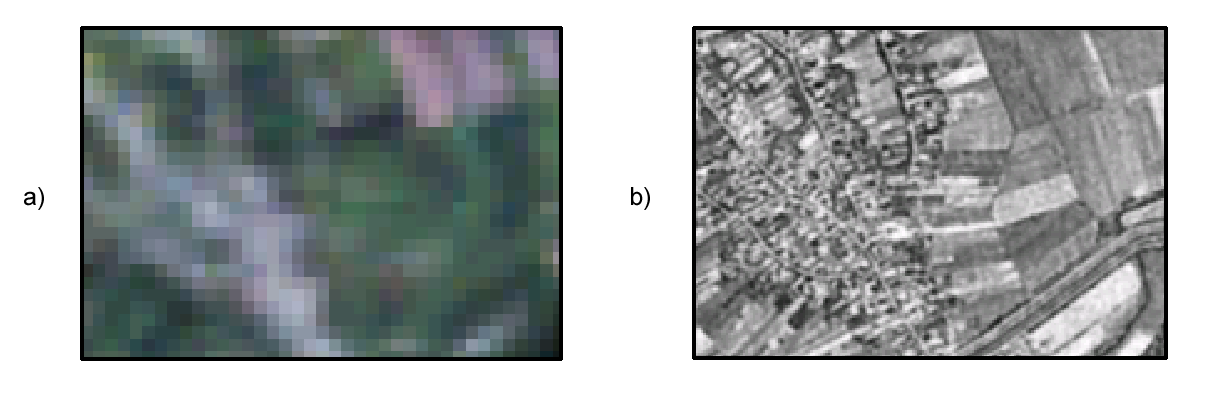
\includegraphics[width=\textwidth]{Tipos_datos/Diferentes_resoluciones.png}
\caption{\small Im�genes de diferente resoluci�n en funci�n del sensor con que han sido obtenidas. Al tener distintos tama�os de p�xel, servir�n para distintos usos dentro de un SIG.}
\label{Fig:Diferentes_resoluciones} 
\end{figure}

Una vez conocemos el formato r�ster, podemos relacionarlo con lo que ya hemos visto relativo a los modelos geogr�ficos. En primer lugar, y por sus propias caracter�sticas, puede pensarse que la representaci�n r�ster es m�s adecuada para variables de tipo continuo que var�an a su vez de forma continua en el espacio geogr�fico. Es decir, es m�s pr�xima al modelo geogr�fico de campos que al de entidades discretas. Esto es as� debido principalmente a que una capa r�ster cubre todo el espacio, y ello favorece el estudio de dicha variabilidad. No obstante, no debe considerarse que el �mbito de las variables continuas y los campos es exclusivo de las capas r�ster. De hecho, de las cuatro representaciones mostradas para el caso de la elevaci�n, solo una de ellas es de tipo r�ster.

S� es cierto, no obstante, que el formato r�ster es especialmente adecuado para el an�lisis de la informaci�n geogr�fica, en especial cuando esta es de tipo continuo. Esto es as� porque el principal elemento de las capas r�ster es, como ya se ha dicho, su estructura sistem�tica. Si a esta le unimos la regularidad que se presenta en la forma m�s extendida de representaci�n r�ster (la de celdas cuadradas regulares), tenemos un modelo �ptimo para el an�lisis, que simplifica en gran medida este y hace m�s sencilla la implementaci�n de los algoritmos correspondientes. Es por ello que, tradicionalmente, los SIG con mayor soporte para datos r�ster han sido aquellos que presentaban a su vez un mayor n�mero de funcionalidades de an�lisis en �reas tales como el estudio del relieve, el an�lisis de costes u otros similares.

No obstante, ello no restringe el alcance del formato. Variables que no resulta tan �ptimo concebir como campos, tales como una red vial, tambi�n puede expresarse como una capa r�ster, como hemos visto en la figura \ref{Fig:Vias_modelos_representacion}.

\subsubsection{El caso de las im�genes}

Un caso especial de capa r�ster son las im�genes, de las que hemos visto ya un ejemplo al tratar el tama�o de celda. Tanto si estas proceden de un sensor digital o bien han sido escaneadas, los sensores correspondientes generan una estructura en forma de malla que se ajusta al modelo de representaci�n r�ster. Este hecho tiene gran importancia, pues facilita el an�lisis conjunto de im�genes y capas de datos con otro tipo de informaci�n, haciendo que este sea sumamente m�s sencillo, al compartir el modelo de representaci�n.

Mientras que, como hemos visto en los ejemplos, una misma informaci�n se puede recoger en formatos r�ster y vectorial, las im�genes se recogen �nicamente en formato r�ster, tanto por ser ese modelo mucho m�s adecuado, como por ser mucho m�s coherente con el tipo de informaci�n y la procedencia de esta.

El concepto de celda en una malla r�ster es el equivalente al de p�xel\footnote{acr�nimo de \emph{picture element}}, bien conocido en el campo de las im�genes digitales. As�, cuando decimos que una c�mara digital tiene tres megap�xeles, queremos decir que captura un total de tres millones de p�xeles. De otra forma, la malla r�ster que se genera tiene tres millones de celdas. Las im�genes con las que trabajamos en un SIG no se diferencian de las que tomamos con una c�mara digital, salvo en el hecho particular de que representan una porci�n de terreno dentro de un sistema de coordenadas dado, pero la estructura es la misma: una malla de celdas (p�xeles).\index{Pixel}

Otra particularidad de las im�genes es la presencia de \emph{bandas}\index{Bandas}. Los valores recogidos en las im�genes indican de forma general la reflectancia\index{Reflectancia} en una determinada longitud de onda (esto se explica con mayor detalle en los cap�tulos \ref{Fuentes_datos} y \ref{Procesado_imagenes}). Puesto que el espectro de radiaci�n\index{Espectro electromagn�tico} puede subdividirse en distintos grupos, los sensores que toman estas im�genes recogen varias capas, una para cada uno de estos grupos. En lugar de almacenarse como un conjunto de capas separadas, es m�s frecuente que lo hagan en una �nica que contiene varias \emph{bandas}, es decir, varios niveles distintos, cada uno de los cuales podr�a constituir por s� mismo una capa r�ster.

Se trata de una diferencia m�s de tipo formal, pero de cierta importancia, puesto que no todos los SIG est�n preparados para manejar capas r�ster con independencia de su n�mero de capas. Im�genes con una �nica banda, o tres, son habituales y soportadas en la mayor�a de implementaciones, mientras que n�meros mayores de bandas no se encuentran soportados en muchos programas.

Todos estos conceptos se extender�n en el cap�tulo \ref{Fuentes_datos}.

\subsection{Modelo vectorial}

El otro modelo principal de representaci�n es el modelo vectorial. En este modelo, no existen unidades fundamentales que dividen la zona recogida, sino que se recoge la variabilidad y caracter�sticas de esta mediante entidades geom�tricas, para cada una de las cuales dichas caracter�sticas son constantes. La forma de estas entidades (su frontera), se codifica de modo explicito, a diferencia del modelo r�ster, donde ven�a impl�cita en la propia estructura de la malla.

Si el modelo r�ster era similar al modelo conceptual de campos, el vectorial lo es al de entidades discretas, pues modeliza el espacio geogr�fico mediante una serie de primitivas geom�tricas que contienen los elementos m�s destacados de dicho espacio. Estas primitivas son de tres tipos: puntos, l�neas y pol�gonos.\index{Primitivas geom�tricas}

\begin{figure}[!hbt]   
\centering
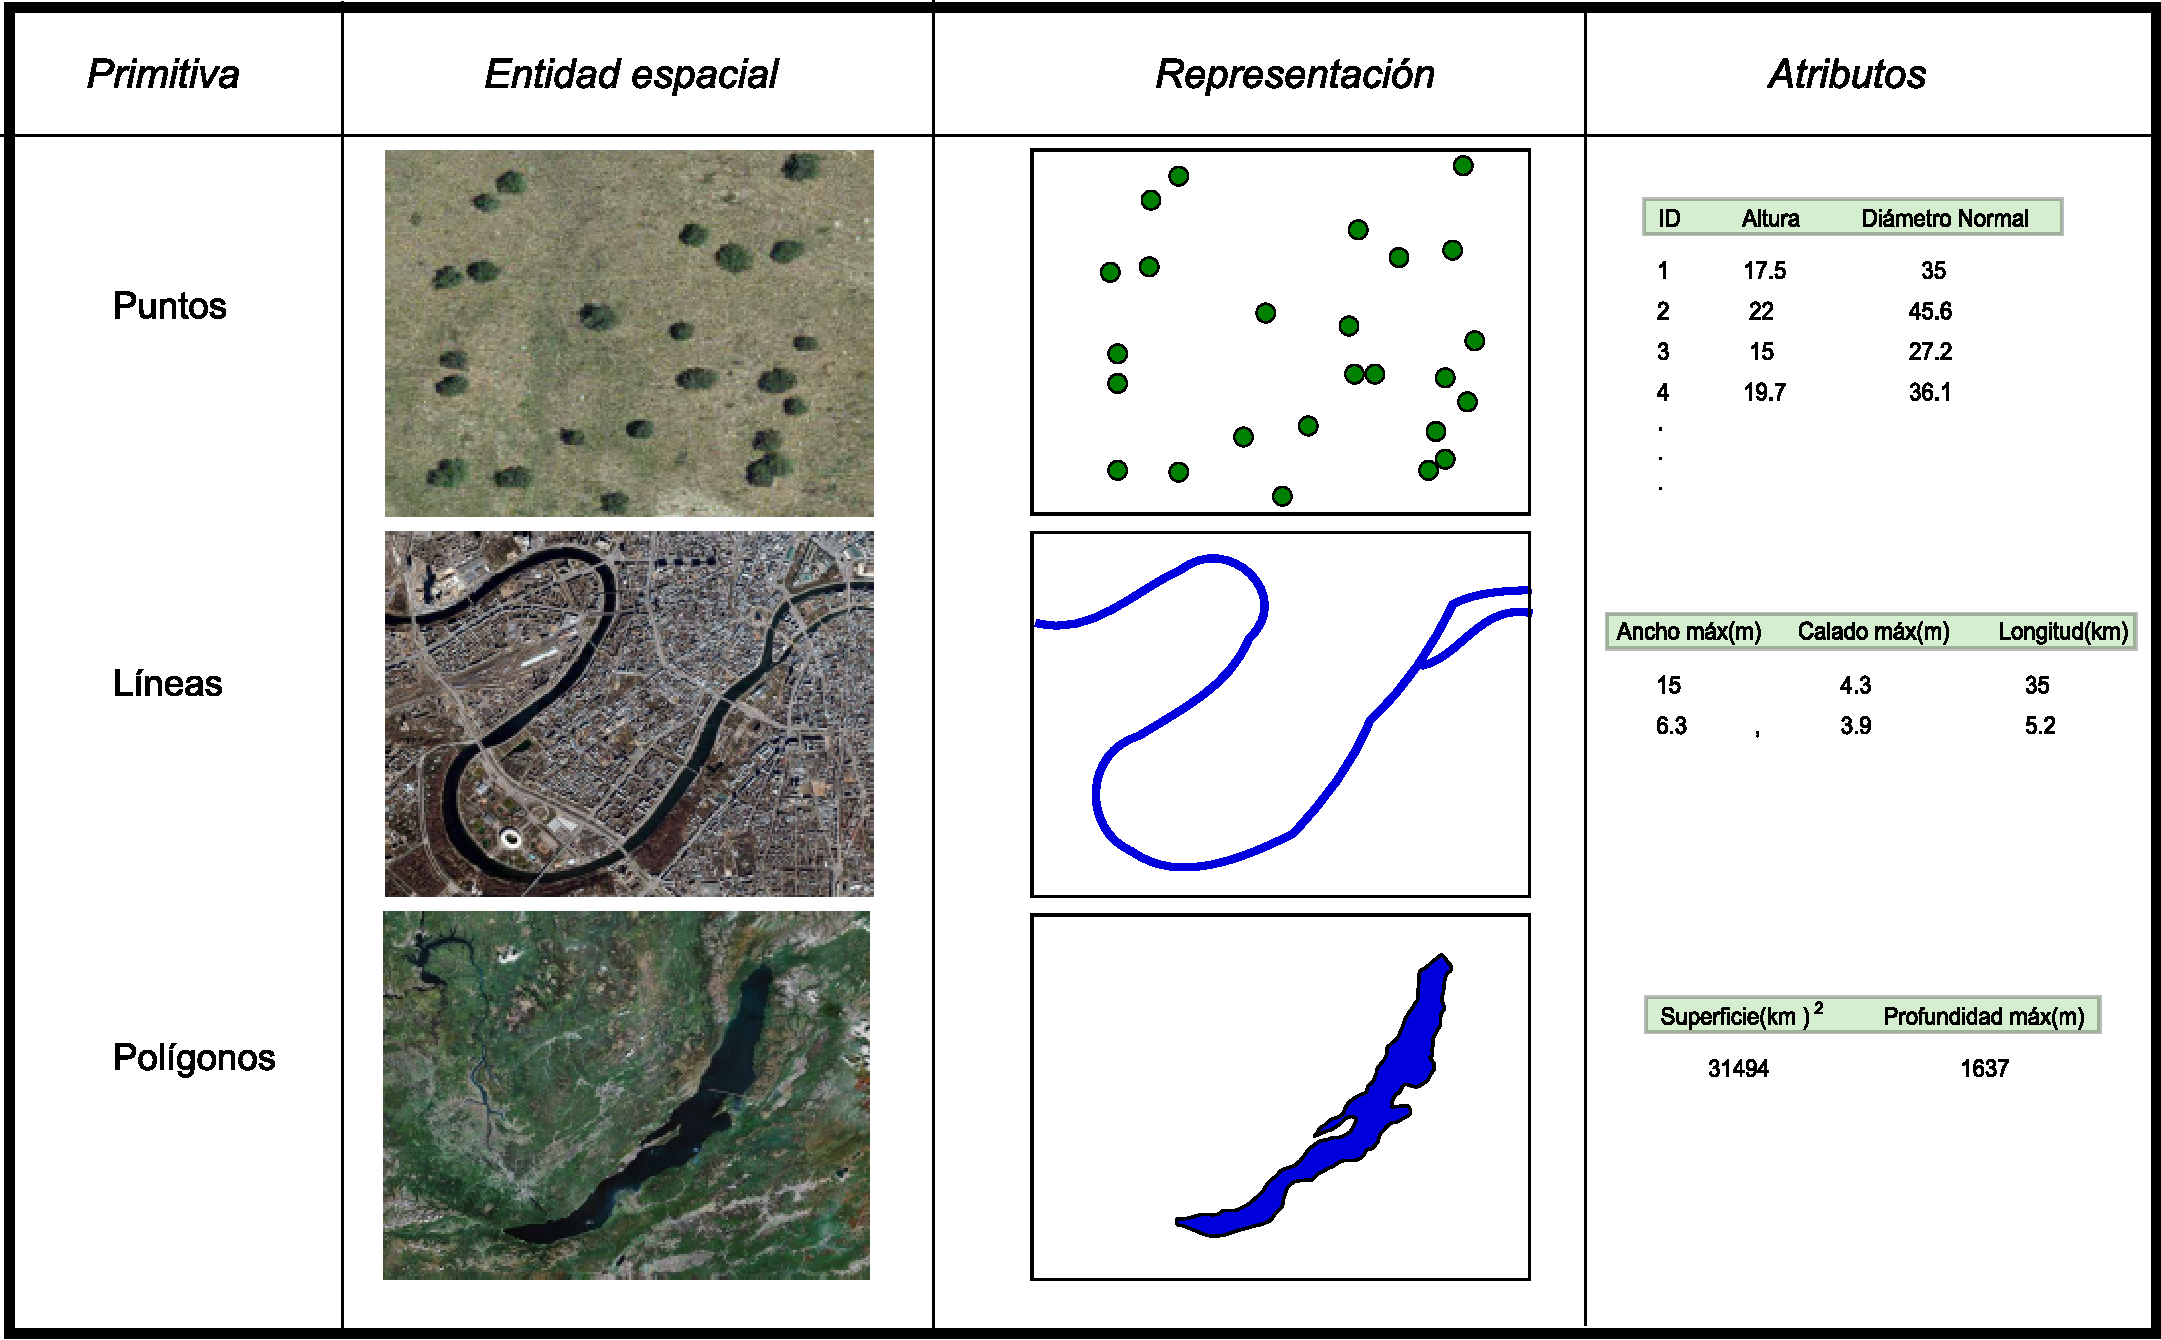
\includegraphics[width=.9\textwidth]{Tipos_datos/Primitivas_vectoriales.pdf}
\caption{\small Primitivas geom�tricas en el modelo de representaci�n vectorial y ejemplos particulares de cada una de ellas con atributos asociados}
\label{Fig:Primitivas_vectoriales} 
\end{figure}

Utilizando puntos, l�neas o pol�gonos, puede modelizarse el espacio geogr�fico si se asocia a estas geometr�as una serie de valores definitorios. La componente espacial de la informaci�n queda as� en la propia primitiva (recoge la forma, posici�n y otras propiedades espaciales), y la componente tem�tica queda en dichos valores asociados (Figura \ref{Fig:Primitivas_vectoriales}).

A la hora de definir las formas geom�tricas b�sicas, todas ellas pueden reducirse en �ltima instancia a puntos. As�, las lineas son un conjunto de puntos interconectados en un determinado orden, y los pol�gonos son l�neas cerradas, tambi�n expresables por tanto como una serie de puntos. Todo elemento del espacio geogr�fico queda definido, pues, por una serie de puntos que determinan sus propiedades espaciales y una serie de valores asociados.

Una �nica entidad (para la cual existir� un �nico conjunto de valores asociados) puede contener varias primitivas. As�, en un mapa mundial en que cada entidad represente un pa�s, y tal y como se ve en la figura \ref{Fig:Casos_particulares_poligonos}, pa�ses como Canad� estar�n representados por m�s de un pol�gono, pues no puede recogerse todo su territorio mediante uno �nico. Todos estos pol�gonos constituyen una �nica entidad, ya que todos perteneces al mismo pa�s y tendr�n el mismo conjunto de valores asociados.

\begin{figure}[!hbt]   
\centering
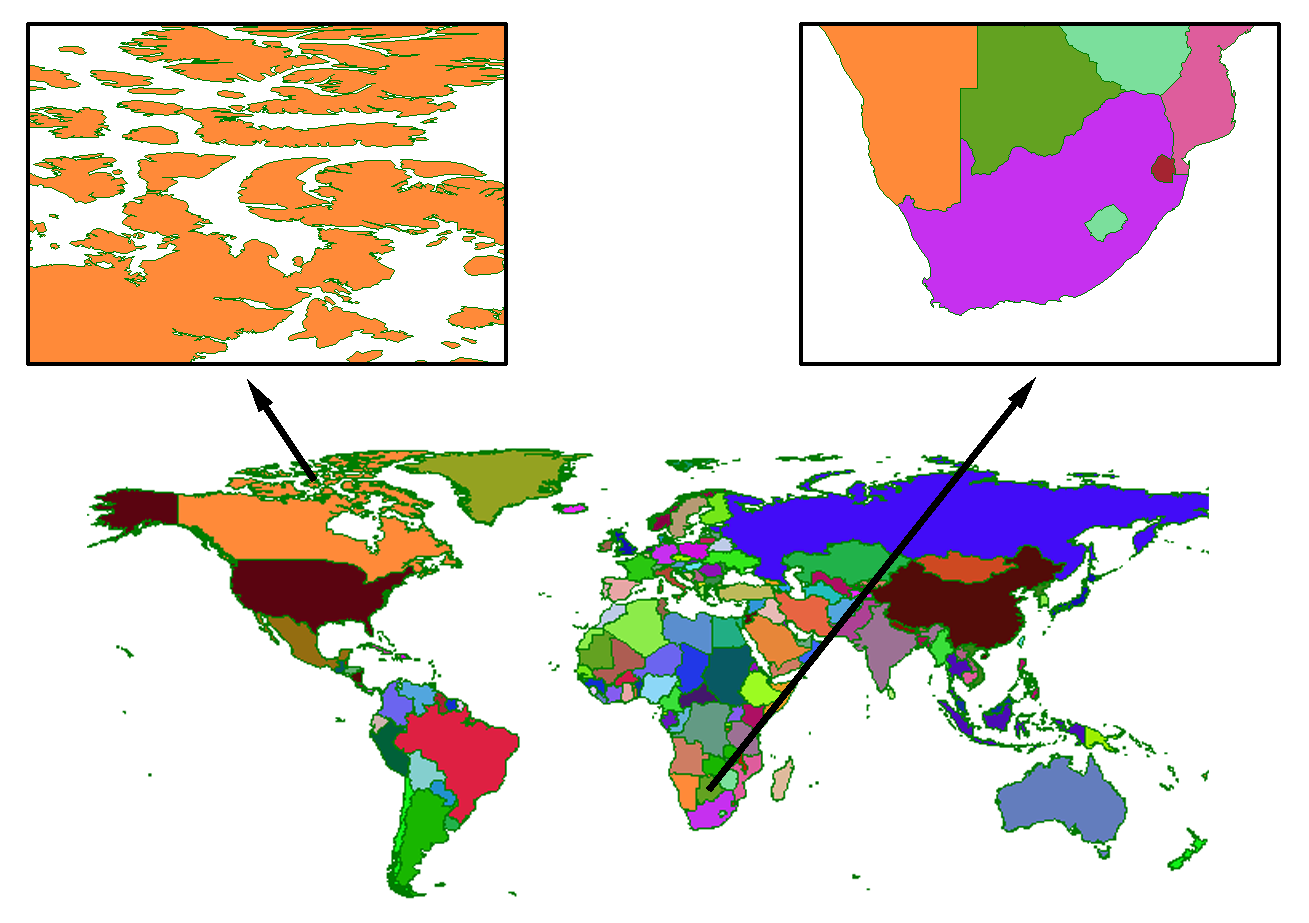
\includegraphics[width=.85\textwidth]{Tipos_datos/Casos_particulares_poligonos.png}
\caption{\small Casos particulares de pol�gonos: a) varios pol�gonos disjuntos en una misma entidad (en este caso, mismo pa�s), b) Pol�gonos con islas (huecos).}
\label{Fig:Casos_particulares_poligonos} 
\end{figure}

\index{Pol�gono!con huecos}\index{Entidades!multiples}

Otro caso particular en las capas de pol�gonos son aquellos pol�gonos con islas (huecos). En este caso, se registran de la misma forma que en el caso de varios pol�gonos disjuntos. Se recogen los propios huecos como pol�gonos independientes, pero recogiendo de alg�n modo tambi�n la circunstancia de que estos pol�gonos no se \emph{suman} a los pol�gonos existentes en esa entidad, sino que se \emph{restan}. As� es, por ejemplo, para el caso del �rea total de pol�gonos de una �nica entidad, ya que el �rea del hueco debe ser restada de la total.

En la figura anterior, vemos como Sud�frica presenta esta situaci�n, ya que dentro del territorio del pa�s hay zonas aislada que no pertenece a Sud�frica, como por ejemplo la que constituye el Reino de Lesotho.\index{Sudafrica}\index{Lesotho, Reino de}

Como se muestra en la figura \ref{Fig:Poligonos_con_huecos}, el conjunto del territorio ocupado por Sud�frica y las zonas interiores que no pertenecen al pa�s no puede verse como un conjunto de pol�gonos sin m�s. Para representar Sud�frica de forma aislada es necesario <<restar>> del pol�gono que engloba todo el territorio los pol�gonos respectivos a los pa�ses interiores. De no hacerlo as�, un c�lculo sencillo tal y como el del �rea de dicho pa�s arrojar� un resultado err�neo, pues considerar� igualmente estas zonas interiores.

\begin{figure}[!hbt]   
\centering
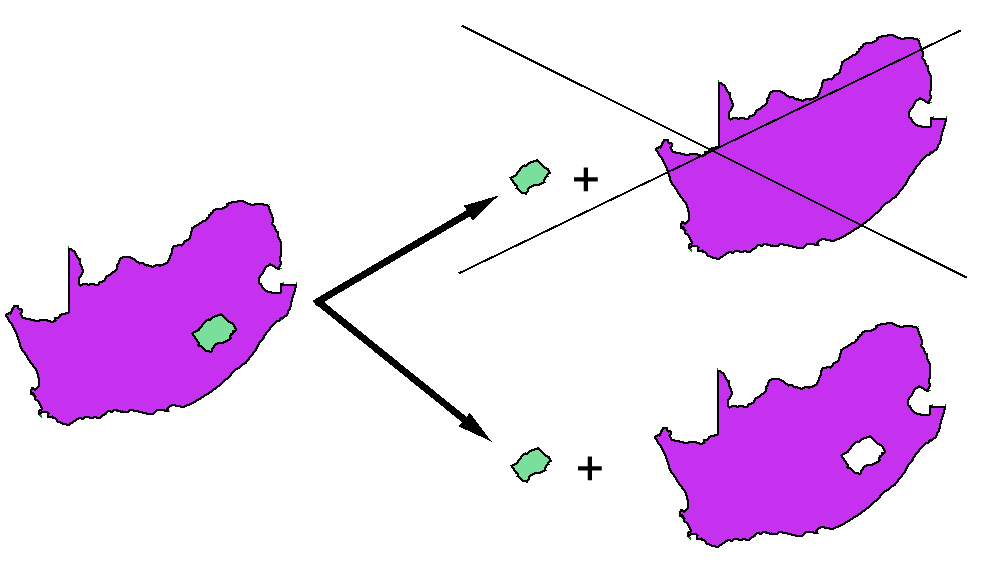
\includegraphics[width=.6\textwidth]{Tipos_datos/Poligonos_con_huecos.png}
\caption{\small Los huecos de un pol�gono han de considerarse como parte de este.}
\label{Fig:Poligonos_con_huecos} 
\end{figure}

En realidad, los huecos se registran como pol�gonos disjuntos que pertenecen a la entidad, aunque en lugar de representar un territorio que se a�ade, representan uno que se <<quita>>. Una forma habitual de hacer esto es almacenar las coordenadas de los v�rtices de estos pol�gonos interiores en sentido inverso, de tal modo que su �rea es negativa. De esta forma, la suma total del �rea de los pol�gonos de la entidad es igual al �rea buscada\footnote{La f�rmula empleada para el c�lculo del �rea de un pol�gono se expone en la p�gina \pageref{Eq:Area_poligono}}.

\index{Pol�gono!�rea de}

Dentro de un SIG, una capa vectorial puede contener un �nico tipo de primitiva. As�, tenemos capas vectoriales de puntos, de l�neas y de pol�gonos, respectivamente. La elecci�n de uno u otro tipo de capa para registrar una variable o conjunto de ellas ha de ser funci�n del tipo de fen�meno que se pretende modelizar con dicha capa o la precisi�n necesaria, entre otros factores. 

Por ejemplo, una capa de puntos puede representar un conjunto de ciudades, cada una de ellas definida como un �nico punto. Sin embargo, puede emplearse una capa de pol�gonos y no recoger una �nica coordenada (correspondiente, por ejemplo, al centro de la ciudad), sino el contorno o los l�mites administrativos de esta. Dependiendo del caso, ser� m�s apropiado elegir una u otra alternativa.

De igual modo, la capa de v�as representada en la figura \ref{Fig:Vias_modelos_representacion} es una capa de l�neas. Cada l�nea, como elemento te�rico de ancho nulo, representa el eje de la v�a. Si se requiere una mayor precisi�n en la definici�n de la superficie de rodadura de dichas v�as, una capa de pol�gonos puede ser utilizada en lugar de una de l�neas.

Lo anterior tiene una evidente relaci�n con los conceptos de escala\index{Escala} y generalizaci�n\index{Generalizaci�n!cartogr�fica} que vimos en el cap�tulo \ref{Fundamentos_cartograficos}.

No debe pensarse que las capas vectoriales, sean del tipo que sean, se emplean �nicamente para recoger fen�menos o elementos cuya forma coincide con la de las primitivas geom�tricas (es decir, puntos para recoger elementos puntuales, l�neas para aquellos elementos con una dimensi�n mucho menor que la otra, y pol�gonos para el caso de superficies). Adem�s de los ejemplos anteriores, debemos recordar que el modelo vectorial tambi�n sirve para representar campos y recoger variables tales como la elevaci�n.

As�, en los ejemplos de la figura \ref{Fig:MDE_modelos_representacion} encontramos capas de puntos, lineas (curvas de nivel) y pol�gonos (TIN), todas ellas empleadas para representar la variable elevaci�n. En ocasiones se emplean las primitivas para recoger objetos reales de forma similar, mientras que en otros casos sirven para plantear un modelo l�gico y recoger variables que no se asemejan de modo alguno a las formas geom�tricas registradas.

A prop�sito de la capa de puntos regulares, cabe pensar que es similar en concepto y forma a la malla r�ster, ya que es regular. Sin embargo, existen dos diferencias importantes: en primer lugar, en la capa de puntos hay zonas en blanco, de las que no sabemos su elevaci�n, mientras que en la malla r�ster las celdas tienen una superficie y cubren en su conjunto todo el espacio. En segundo lugar, si tenemos esa capa de puntos en un SIG, esta va a contener las coordenadas particulares de cada punto, ya que en s� las capas vectoriales no son regulares (pueden guardar alguna regularidad, pero no necesariamente), y por tanto es necesario, como hemos visto, registrar expl�citamente sus coordenadas. De modo similar podr�amos hacer una capa de pol�gonos cuadrados, pero seguir�a sin ser una malla r�ster, m�s a�n si careciera de un elemento que veremos en breve: la topolog�a. \index{Topolog�a}

\subsubsection{La componente tem�tica en el modelo vectorial}

La forma en la que los modelos de representaci�n separan las dos componentes de la informaci�n geogr�fica hemos visto que es bien distinta. En el modelo r�ster se tiene un conjunto de valores (la componente tem�tica), los cuales guardan una estructura dada, la cual por s� misma establece su disposici�n en el espacio (la componente espacial). En el vectorial, por su parte, la componente espacial se recoge expl�citamente seg�n una serie de puntos, la cual puede ser m�s o menos compleja en funci�n de la complejidad de la entidad a representar o el detalle con que se recoja. A este conjunto de puntos se le relaciona despu�s con una serie de valores, que son los que definen las propiedades de la entidad.

Estos valores, los \emph{atributos}, a diferencia del caso r�ster, suelen ser m�ltiples. Por ejemplo, dada una capa vectorial de pa�ses, podemos recoger valores asociados a cada pa�s tales como su superficie, su poblaci�n, el Producto Interior Bruto, el nombre de su capital o el idioma que se habla. Todo este conjunto de valores se asocian a una �nica copia de la componente espacial, y esta no debe repetirse para recoger cada uno de esos par�metros. En el modelo r�ster, si tenemos $n$ capas distintas, en realidad estamos almacenando $n$ veces la componente espacial.
\index{Atributos!de una capa vectorial}

Por esta estructura particular, la componente tem�tica se presta especialmente a almacenarse en una base de datos, siendo en la actualidad las m�s extendidas las denominadas \emph{bases de datos relacionales}. Estas bases de datos se \emph{enlazan} a la componente espacial y permiten una serie de operaciones(ver cap�tulo \ref{Consultas}) y un manejo ventajoso de los \emph{atributos}. Existen, por tanto, dos realidades: la relativa a la componente geogr�fica y la base de datos que gestiona los atributos, la cual permite an�lisis y operaciones independientes, del mismo modo que si no existir� una localizaci�n asociada a dichos atributos. Estas realidades pueden estar muy separadas, gestion�ndose en aplicaciones distintas y almacen�ndose en ficheros diferentes, con lo cual existe una divisi�n formal mucho m�s acusada que en el caso de las capas r�ster, que se asemejan m�s a unidades de informaci�n autocontenidas.

En el caso de las capas r�ster, no es necesario recurrir a una base de datos, y simplemente la representaci�n del conjunto de valores de la variable en las distintas celdas sirve para el almacenamiento, an�lisis y manejo de la informaci�n. Como indica \cite{Heywood1998Longman}, esta forma de \emph{conectar} las componentes espacial y tem�tica es apta para el an�lisis, pero el manejo de los atributos requiere la presencia de una base de datos.\index{Base de datos}

El establecimiento de las bases de datos, su manejo y su implementaci�n dentro de un SIG es un tema altamente complejo. La forma en que el manejo de la componente tem�tica y la gesti�n de la base de datos se establecen, as� como la imbricaci�n de la una en la otra, es la materia exclusiva del cap�tulo \ref{Bases_datos}, donde todos estos temas se desarrollar�n con profundidad.

\subsubsection{Topolog�a}\label{Topologia}

\index{Topolog�a}

Un elemento particular del modelo de representaci�n vectorial es la \emph{topolog�a}. En t�rminos matem�ticos la topolog�a estudia las caracter�sticas de los objetos geom�tricos que no var�an al aplicar una transformaci�n topol�gica tal como, por ejemplo, una transformaci�n af�n\index{Transformaci�n!af�n}. Si tomamos un mapa y lo distorsionamos, los �ngulos, las superficies y las distancias se ven afectadas. Sin embargo, otras propiedades tales como la adyacencia entre elementos o las relaciones entre estos se conservan. Por ejemplo, si una ciudad est� dentro de una determinada provincia en un determinado mapa, no existe forma de distorsionar esta para lograr que dicha ciudad se encuentre fuera de la provincia.

En el �mbito de los SIG se entiende la topolog�a desde un punto de vista menos estricto y m�s funcional. En general, se dice que una capa de informaci�n tiene topolog�a si en ella se almacenan de alg�n modo las relaciones entre los distintos elementos que la componen. En caso contrario, la capa es de tipo puramente cartogr�fico, ya que los elementos que contiene no presentan relaci�n entre s�, o al menos esta relaci�n no est� almacenada junto a la propia informaci�n de estos elementos.

En una capa r�ster, las relaciones topol�gicas vienen impl�citas en el propio modelo r�ster, y son ajenas a la informaci�n como tal, dependiendo de la estructura de la malla de datos en s�. En el modelo vectorial, sin embargo, se recoge la informaci�n relativa a cada elemento de forma individual, y si las relaciones existentes no se registran de modo explicito, no se tendr� posteriormente informaci�n sobre ellas.

Disponer de topolog�a en una capa vectorial es de gran importancia a la hora de llevar a cabo ciertos tipos de an�lisis, as� como otros tales como la edici�n de los propios datos geogr�ficos. La topolog�a no aporta beneficio a la hora de representar una capa, pero s� a la hora de llevar a cabo an�lisis sobre ella \cite{Herring1987Autocarto}. 

En la figura \ref{Fig:Topologia_edicion} se puede observar la diferencia existente entre editar una capa de pol�gonos con topolog�a y una sin ella. En el primer caso, la informaci�n contenida en la capa antes de su edici�n nos informa no solo de la forma de cada pol�gono, sino tambi�n del hecho de que ciertos pol�gonos comparten bordes comunes y de que el conjunto de ellos cubre el espacio de forma completa (constituyen una teselaci�n\index{Teselaci�n}). As�, al modificar un punto en uno de los pol�gonos, todos aquellos pol�gonos adyacentes que comparten dicho punto modifican tambi�n su per�metro. Las capacidades de edici�n implementadas en el Sistema de Informaci�n Geogr�fica hacen uso de la informaci�n topol�gica a la hora de editar geometr�as. En el segundo caso, sin embargo, esta informaci�n no existe, y no se pueden alterar los pol�gonos adyacentes, perdi�ndose la teselaci�n completa del espacio.

\begin{figure}[!hbt]   
\centering
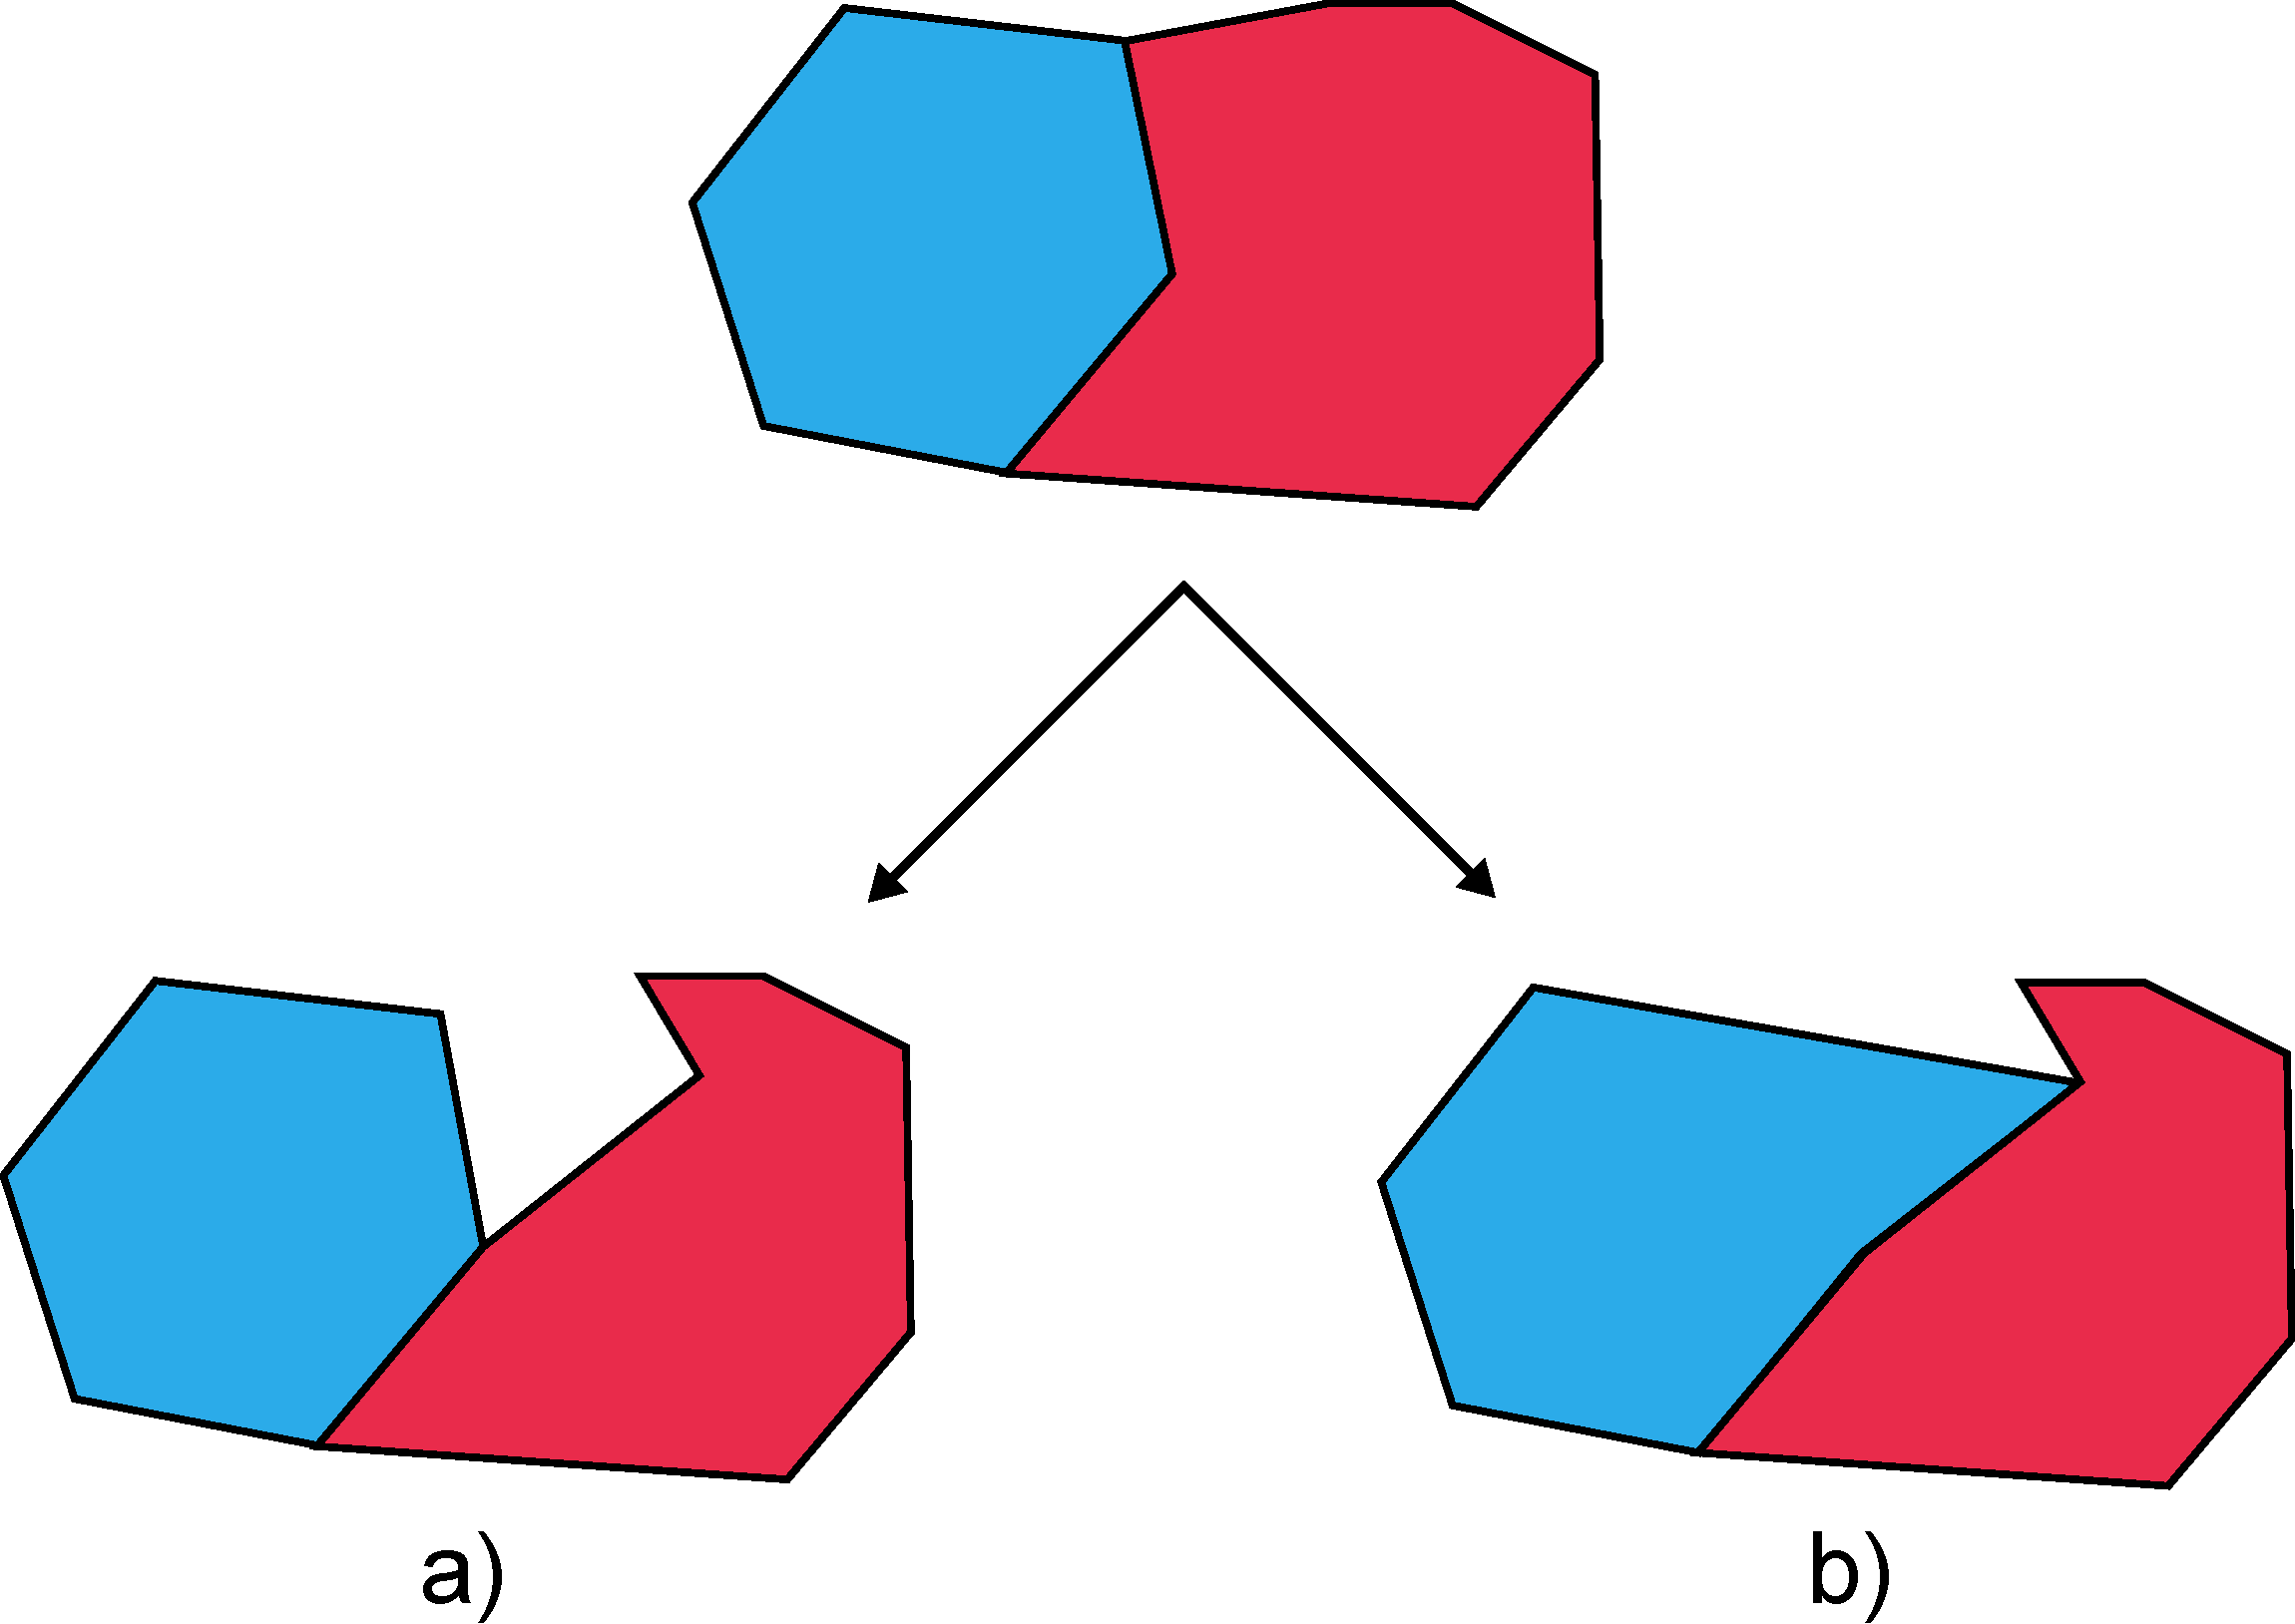
\includegraphics[width=.6\mycolumnwidth]{Tipos_datos/Topologia_edicion.pdf}
\caption{\small Diferencias entre la edici�n (desplazamiento de un punto) no disponiendo de topolog�a (a) o con ella (b).}
\label{Fig:Topologia_edicion} 
\end{figure}

La topolog�a es en este caso un elemento que contribuye a la calidad de los datos, pues mantiene la coherencia espacial de estos y evita la aparici�n de elementos tales como pol�gonos de muy peque�o tama�o, frecuentes en la digitalizaci�n de entidades debido a las peque�as imprecisiones que se presentan en el proceso, y que causan la presencia de falsos solapes entre pol�gonos.

No obstante, no todos los SIG incorporan capacidades de manejo y an�lisis de capas vectoriales con topolog�a, y son menos a�n los que implementan capacidades para crear dicha topolog�a. En general, estas han quedado reservadas a las aplicaciones de alta gama, y el manejo de informaci�n vectorial en los SIG de escritorio no incluye de forma general lo relativo a la topolog�a.

Otro ejemplo de proceso en el que se hace necesario el disponer de capas con topolog�a es el an�lisis de redes (este se detalla en el cap�tulo\index{Redes!an�lisis de} \ref{Analisis_redes}). Un mero conjunto de elementos geom�tricos (l�neas en este caso), no nos da informaci�n sobre los posibles enlaces entre las v�as que quedan representadas. Los puntos donde se cruzan dos v�as pueden ser cruces o rotondas (es decir, puede pasarse de una v�a a otra, existiendo conexi�n entre ellas), o bien pasos elevados o subterr�neos donde una de las v�as pasa por encima de la otra (y por tanto no existe comunicaci�n entre ambas). Las circunstancias son muy distintas en funci�n del tipo de cruce que exista, y por ello es imprescindible conocer esta informaci�n para efectuar un an�lisis de redes correcto. 

Otro elemento que no se puede recoger sin topolog�a son las direcciones de circulaci�n. Habr� v�as que puedan recorrerse en ambos sentidos, mientras que habr� otras que solo permitan movimiento de tr�fico en una direcci�n. Saber en qu� direcci�n podemos recorrer una v�a es vital para poder plantear cualquier tipo de an�lisis, y esta es una informaci�n de la que no disponemos si nuestra red viaria no ha sido representada mediante un modelo con topolog�a.

Estas circunstancias se recogen de forma esquem�tica en la figura \ref{Fig:Topologia_vias}

\begin{figure}[!hbt]   
\centering
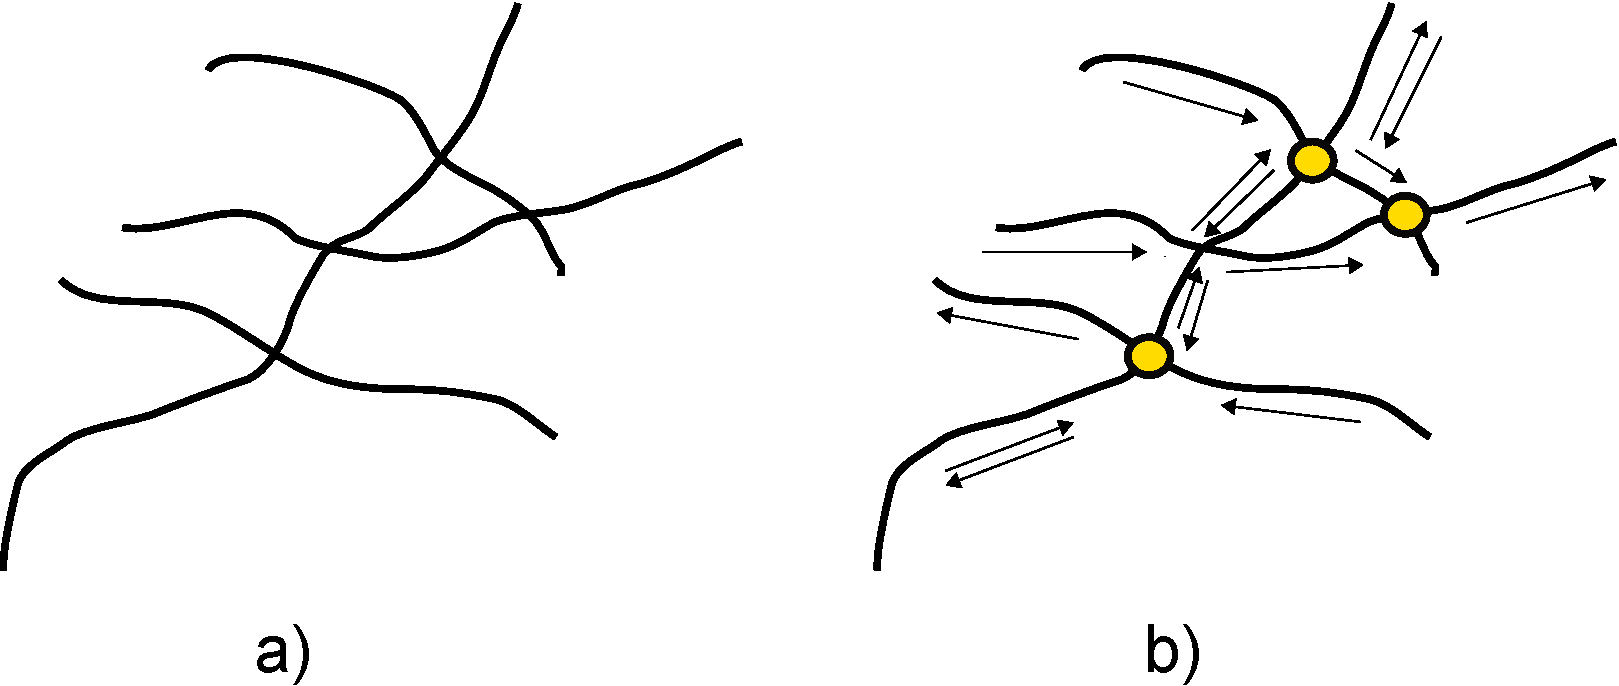
\includegraphics[width=.6\mycolumnwidth]{Tipos_datos/Topologia_vias.pdf}
\caption{\small Capa de v�as de comunicaci�n sin topolog�a (a) o con ella (b). Los puntos en este segundo caso indican conexiones entre vias, y son una representaci�n visible de la topolog�a existente. Las flechas indican la direcci�n de circulaci�n y, al igual que sucede con las conexiones, solo est�n presentes si existe topolog�a}
\label{Fig:Topologia_vias} 
\end{figure}


Aunque, como se ha mencionado, las capas r�ster en cierta forma contienen informaci�n topol�gica (se conoce la relaci�n de adyacencia entre las distintas celdas), esta es \emph{d�bil}, y no suficiente para an�lisis complejos como el de redes donde existen distintos elementos como los mencionados cruces o las direcciones de circulaci�n. Aparte de la inherente peor disposici�n del modelo de representaci�n para recoger una entidad espacial tal como una red, el modelo r�ster no es �ptimo para recoger la necesaria informaci�n topol�gica al respecto. Existen algunos intentos de adaptarlo a estas circunstancias (v�ase, por ejemplo \cite{Husdal2000MsC}), pero en general no se encuentran implementados de forma habitual.

\index{Topolog�a!sobre capas r�ster}

\subsubsection{Modelo vectorial sin topolog�a (\emph{spaguetti})}

\index{Spaguetti@\emph{Spaguetti}}

El modelo de datos vectorial almacena la informaci�n geogr�fica mediante una serie de entidades geom�tricas (lineas, puntos, pol�gonos), y una informaci�n asociada (los atributos). La forma en que estas geometr�as se recogen es, no obstante, �nica, y en funci�n del enfoque adoptado, permitir� el almacenamiento o no de propiedades topol�gicas relativas a dichas geometr�as. Se tienen as� \emph{submodelos} de representaci�n, cada uno de ellos con un esquema distinto de almacenamiento de los elementos individuales que constituyen una capa r�ster.

Con independencia del submodelo, en todo caso las entidades se recogen mediante las coordenadas de sus puntos, pues como ya se vio toda entidad es reducible a un conjunto de puntos. La diferencia estriba en la forma en que dichos puntos se asocian a la representaci�n de una entidad dada. Para el caso de una capa de puntos, no existe diferencia alguna, pero en el caso de l�neas o pol�gonos s� la hay.

En el tipo m�s simple, se recogen �nicamente las propiedades geom�tricas de cada entidad, almacenando para cada una de ellas el conjunto de puntos individuales que la componen. Esto aporta toda la informaci�n necesaria sobre la entidad, pero deja de lado la topolog�a. Algunas propiedades topol�gicas pueden calcularse, tales como saber si un punto esta contenido dentro de un pol�gono o si dos rectas se cruzan, pero para otras no se dispone de informaci�n suficiente. As�, aunque podamos saber si dos l�neas se cruzan, no podemos saber si este cruce implica una conexi�n real entre ellas de forma que pueda pasarse de la una a la otra o no, como vimos en la figura \ref{Fig:Topologia_vias}.

Esta forma de recoger las entidades vectoriales es similar a la que encontramos en un mapa cl�sico, en el cual podemos conocer la forma de un �rea dada o el recorrido que sigue una determinada carretera, pero no las relaciones existentes. �nicamente disponemos del trazo con el que se han dibujado estos elementos. Por esta raz�n, y como se ha dicho, un modelo vectorial sin topolog�a es perfectamente v�lido para la representaci�n de cualquier tipo de informaci�n en formato vectorial, pero no tanto para su an�lisis.

El almacenamiento de entidades basado en una mera lista de coordenadas de cada entidad se conoce popularmente como \emph{spaghetti}, pues si pensamos en una capa de lineas sin topolog�a que se entrecruzan en el espacio, esta se asemejan en cierta forma a un ca�tico plato de \emph{spaguettis} sin orden ni relaci�n entre ellos.

La mayor ventaja de este modelo es su simplicidad, raz�n por la cual es la habitual en muchos de los SIG m�s populares. Para muchos usuarios, es suficiente trabajar con datos vectoriales sin topolog�a, pues las labores frecuentes que desarrollan, tales como consultas (cap�tulo \ref{Consultas}) o creaci�n de mapas derivados, no requiere conocer las relaciones topol�gicas existentes.\index{Consultas}

Gran parte de las operaciones que se desarrollan en un SIG no requieren topolog�a, y por ello no es necesario asumir siempre el coste que implica trabajar con ella (mayor complejidad en general). Es por ello que incluso aquellos SIG que s� poseen la capacidad de trabajar con topolog�a, tambi�n disponen de formas de trabajar sin ella, empleando datos que carecen de topolog�a. Esto es as� tambi�n debido a que mucha informaci�n disponible no incluye topolog�a, ya que o bien esta no se incorpor� en el momento de la digitalizaci�n, o bien el formato de fichero en el que se almacen� no soportaba la inclusi�n de topolog�a. %********(vease apartado \ref{Formatos_fichero} para m�s detalles sobre este aspecto)

En otros casos, la propia naturaleza de la variable que recogemos puede requerir ser almacenada sin topolog�a, o bien puede ser que no existan relaciones topol�gicas que representar. Una capa de pol�gonos en las cuales se recojan las �reas de influencia de unos determinado fen�menos puntuales pueden perfectamente solaparse. No existe en este caso esa relaci�n que hace que el conjunto de pol�gonos que las representan cubra la totalidad del espacio y cada punto pertenezca a una sola entidad. En este caso, un punto puede estar afectado por uno, varios o ninguno de dichos fen�menos puntuales, y por tanto pertenecer a una, varias o ninguna de las entidades poligonales que representan sus respectivas �reas de afecci�n. Al modificar una de ellas (por ejemplo, si el fen�meno puntual que la origina var�a su intensidad), las dem�s geometr�as no deber�an verse afectadas. No existe como tal una relaci�n que deba recogerse en forma de topolog�a.

\subsubsection{Con topolog�a}

La alternativa al modelo vectorial sin topolog�a (el que denomin�bamos \emph{spaguetti}) es el almacenamiento expl�cito de las relaciones topol�gicas, recogiendo las coordenadas de los puntos que constituyen cada entidad, pero no mediante una simple lista para cada una de ellas. Recogiendo de forma individual toda la informaci�n espacial correspondiente a cada entidad, la topolog�a se pierde, pues no se considera al conjunto de entidades como un conjunto en el cual existen relaciones internas, sino como una simple colecci�n de cosas. Para recoger la topolog�a es necesario considerar todos los puntos que constituyen las entidades, y despu�s \emph{formar} las entidades a partir de ese todo de puntos, considerando en el proceso que un mismo punto puede pertenecer a varias entidades. Esto es lo que se denomina frecuentemente un \emph{diccionario de puntos}, ya que contiene las definiciones de estos (sus coordenadas) y en base a ellos se construyen las distintas geometr�as. \index{Diccionario de puntos}

Esta forma de considerar el conjunto de entidades evita, adem�s, la redundancia en los datos.\index{Redundancia} Por ejemplo, para el caso mostrado en la figura \ref{Fig:Topologia_edicion}, y en caso de no tener topolog�a, el punto que es movido est� almacenado dos veces, una por cada pol�gono. Al desplazarlo, solo se modifica una copia de dicha coordenada, la que pertenece al pol�gono editado, mientras que la otra permanece en su lugar. Si se dispone de topolog�a, este punto se almacena una �nica vez, y al desplazarse se modifican las fronteras de todos los elementos (lineas o pol�gonos, seg�n el caso) cuya frontera incluye dicho punto.

La denominaci�n de \emph{diccionario de puntos} que se mencionaba anteriormente es muy reveladora en este sentido. Si los puntos son como las palabras de un diccionario y los pol�gonos como frases o p�rrafos, basta pensar en lo poco pr�ctico que ser�a escribir una frase en la que debiera definirse cada palabra al introducirla en dicha frase. Resulta mucho m�s adecuado (y ahorra esfuerzos al escritor), utilizar las palabras simplemente, y despu�s definir estas en un diccionario en caso de que el lector no las conozca y necesite una referencia. Con el caso de los puntos sucede algo similar.

Existen diversos modelos para almacenar tanto las propias geometr�as como sus relaciones inherentes, dos de los cuales se muestran en la figura \ref{Fig:Modelos_topologia} mediante sendos ejemplos en los que se codifican pol�gonos y l�neas.

\begin{figure}[!hbt]   
\centering
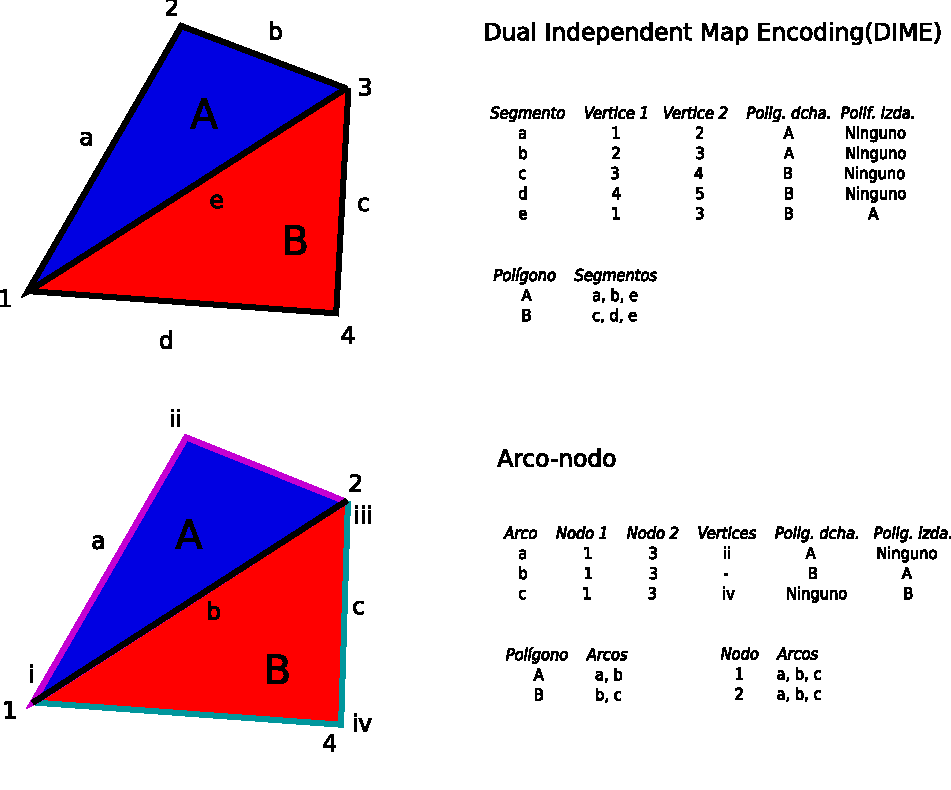
\includegraphics[width=.8\textwidth]{Tipos_datos/Modelos_topologia.pdf}
\caption{\small Dos modelos para representar la topolog�a de l�neas y pol�gonos. a) DIME, b) arco--nodo.}
\label{Fig:Modelos_topologia} 
\end{figure}

El primero de estos modelos es un modelo de car�cter hist�rico denominado DIME (\emph{Dual Independent Map Encoding})\index{Dual Independent Map Encoding}, desarrollado originalmente por el \emph{US Bureau of the Census}\index{US Bureau of the Census}, y posteriormente mejorado en el modelo TIGER, empleado para la digitalizaci�n de cartograf�a urbana. El segundo es el modelo \emph{arco--nodo}, probablemente el m�s difundido y popular en la actualidad, aunque a este respecto los planteamientos existentes son muy variados.\index{Modelo!arco--nodo}

En este modelo existen dos unidades fundamentales: Los nodos, que son puntos donde se \emph{conectan} varias l�neas; y los \emph{arcos}, que son lineas entre dos nodos. Estas l�neas no han de ser rectas, ya que pueden contener en su recorrido \emph{v�rtices}. Los v�rtices son en realidad los puntos que solo pertenecen a una entidad, mientras que los nodos pertenecen a varias de ellas.\index{V�rtices}\index{Arco}

Una capa de l�neas se describe como un conjunto de arcos y nodos, de forma que, atendiendo a los nodos como enlaces entre las l�neas, se pueden conocer las relaciones entre ellas. En el caso de pol�gonos, estos se forman con conjuntos de arcos que delimitan las fronteras. Los pol�gonos que son adyacentes comparten uno o m�s arcos, quedando establecida as� mediante ellos la relaci�n topol�gica.

En el caso del modelo DIME, sin embargo, vemos que cada linea recta entre dos puntos se trata como una unidad, es decir, que todos los v�rtices son considerados como nodos y los arcos se componen siempre de una sola l�nea. El arco es en realidad un segmento. En ambos casos, no obstante, cada arco tiene un inicio y un final ---y por tanto una direcci�n---, y puede definirse un lado derecho y otro izquierdo seg�n se avanza en dicha direcci�n. Como puede verse, tambi�n en ambos modelos se recoge expl�citamente qu� pol�gono, en caso de haber alguno, se sit�a a cada lado del arco.

La informaci�n que se recoge seg�n estos modelos, vemos que se divide en bloques seg�n los distintos niveles, desde los puntos, que han de recogerse en un diccionario de puntos (aunque este no queda reflejado en las tablas de la figura), pasando por los segmentos o arcos, y hasta los pol�gonos, definidos estos en base a los anteriores.

Con independencia del modelo, y sin entrar en m�s detalles, todos estos elementos en conjunto sirven para recoger las relaciones existentes entre los elementos, de tal modo que pueden llevarse a cabo tambi�n aquellas operaciones que no dependen exclusivamente de la posici�n, sino asimismo de otra serie de propiedades.

Dentro de los modelos existentes, encontramos asimismo variaciones en funci�n de la tarea principal que se desee realizar. La eficiencia de cierto tipo de c�lculos puede aumentarse notablemente si se elige un modelo de representaci�n �ptimo, como podemos ver si analizamos una de las operaciones m�s comunes: el c�lculo de rutas �ptimas entre dos puntos (los detalles sobre este c�lculo se exponen en el cap�tulo \ref{Costes}, aqu� por el momento �nicamente mostraremos sus implicaciones en los modelos de representaci�n).


\index{Ruta �ptima}

Para calcular la ruta �ptima entre dos puntos dados de una red necesitamos conocer qu� nodos de la red est�n conectados entre s� y por qu� v�as est�n conectados, ya que las caracter�sticas de estas condicionan el movimiento. La informaci�n necesaria para este c�lculo puede almacenarse perfectamente seg�n un modelo arco--nodo como el que ya conocemos, pero considerando las particularidades del an�lisis que queremos realizar, existen otros modelos m�s apropiados. 

Por ejemplo, se puede tener en cuenta que los v�rtices de un nodo no tienen relevancia alguna. Si el tr�nsito se realiza entre dos nodos, a efectos del c�lculo es indiferente que el tramo que los une tenga unos u otros v�rtices. Lo �nico que importa es saber que existe un tramo que los conecta y las caracter�sticas de ese tramo como, por ejemplo, el tiempo que cuesta recorrerlo o si conecta el nodo A con el B y el B con el A o solo lo hace en una de las direcciones anteriores. Por ello, en el caso del an�lisis de redes, la clave reside en almacenar de forma eficiente los nodos y las relaciones, pues estos son los elementos esenciales para efectuar los c�lculos

Algunos modelos empleados com�nmente para el almacenamiento de redes son los siguientes \cite{NCGIA}:

\begin{itemize}
\item Matriz de incidencias arco--nodo
\item Matriz de adyacencias nodo--nodo
\item Listas de adyacencia
\item Estrella directa e inversa\footnote{Forward and reverse star}
\end{itemize}

\index{Matriz!de incidencias}\index{Matriz! de adyacencias}\index{Listas de adyacencia}\index{Estrella directa e inversa}\index{Forward and reverse star}

La matriz de adyacencias nodo--nodo es sumamente sencilla, ya que simplemente, para un n�mero $n$ de nodos, contiene una matriz de tama�o $n\times n$, en la que cada elemento ($i,j$) indica la existencia o no de conexi�n entre los nodos $i$ y $j$ y la naturaleza de dicha conexi�n. Si el elemento es igual a cero indica que no existe posibilidad de desplazarse directamente del nodo $i$ al nodo $j$. En caso contrario, el valor es igual a la propiedad que se desee recoger del tramo, por ejemplo el tiempo que se tarda en recorrer o la velocidad m�xima a la que puede hacerse ese recorrido.

La gran ventaja de este m�todo es su gran sencillez, que deriva en sencillas implementaciones de los algoritmos correspondientes.

El m�todo de estrella directa e inversa, por su parte, no es tan sencillo (una descripci�n algo m�s detallada puede encontrarse en \cite{NCGIA}), pero, no obstante, es el m�s eficaz \cite{Ahuja1993Prentice}, y sus tiempos de c�lculo asociados son los menores de entre todos los anteriores. 

M�s all� de los detalles particulares del modelo de representaci�n, lo importante es tener presente que existen diversas formas de representar el dato geogr�fico, y que cada una de ellas tiene sus ventajas e inconvenientes en relaci�n con la funci�n que los datos hayan de desempe�ar.

\subsubsection{TIN}\label{TIN}

Hemos visto c�mo una capa vectorial con topolog�a nos sirve para modelizar ventajosamente elementos como una red de v�as o una teselaci�n\index{Teselaci�n} del espacio en, por ejemplo, diferentes clases de usos de suelo. Adem�s de esto, la incorporaci�n de topolog�a sirve para mejorar la representaci�n de campos mediante modelos vectoriales, permitiendo la aparici�n de modelos como los TIN, ya presentados con anterioridad. 

Un TIN\index{Triangulated Irregular Network (TIN)} \cite{Peuker1978ASP} es una red formada por un conjunto de tri�ngulos interconectados, cada uno de los cuales representa a una zona de caracter�sticas homog�neas en lo que a la variable estudiada respecta. Debido a esto, y como puede verse en la figura \ref{Fig:MDE_modelos_representacion}, el n�mero de tri�ngulos var�a seg�n las caracter�sticas propias de la zona. 

En aquellos lugares en los que se d� una gran variaci�n (en caso de recoger el relieve ser� en las �reas m�s abruptas), se utiliza un gran n�mero de tri�ngulos para recoger toda esa variabilidad. Cuando, por el contrario, los valores no var�an de forma tan notable (zonas de relieve m�s llano), pueden emplearse menos tri�ngulos. Puesto que cada tri�ngulo est� formado, como todo pol�gono, por puntos, podemos decir que se necesitan menos puntos para almacenar un terreno si este es llano que si este es muy abrupto.

Cada tri�ngulo tienen unas propiedades constantes, como corresponde al modelo vectorial. En particular, se considera habitualmente que todos los puntos dentro de un mismo tri�ngulo constituyen un plano, con una pendiente y una orientaci�n fija por tanto.

La topolog�a del modelo permite llevar a cabo an�lisis diversos sobre un TIN, ya que para cada tri�ngulo se tiene conocimiento de cu�les son los adyacentes a este, y es en el an�lisis de dichos adyacentes en el que se basan gran parte de los algoritmos. Este an�lisis resulta sencillo de implementar en una capa r�ster, pues la propia estructura de la misma informa directamente de las celdas circundantes, pero en el caso vectorial requiere la presencia de topolog�a para plantear un esquema similar de operaci�n. 

El an�lisis de los TIN no se desarrolla en detalle en este libro, pero resulta interesante recalcar en este punto que resulta posible de igual modo, y ello es debido a la presencia de topolog�a en la propia estructura del modelo de representaci�n.

Las particularidades del TIN hacen que existan sub--modelos principales para almacenar el conjunto de tri�ngulos, distintos del habitual arco--nodo, y pensados espec�ficamente para responder a las necesidades que los TIN demandan como modelos vectoriales para representar variables continuas (en este sentido, es algo muy similar al caso que ve�amos anteriormente de las redes). Estos modelos son dos, principalmente:

\begin{itemize}
 \item Almacenamiento de los tri�ngulos uno por uno, cada uno con las coordenadas de todos sus tres puntos (coordenadas tridimensionales, no planas) y un c�digo de identificaci�n, y almacenamiento de los c�digos de los tri�ngulos adyacentes.
\item Almacenamiento de los v�rtices y un c�digo para cada uno de ellos, as� como los c�digos de los v�rtices a los que se encuentra conectado, en un orden establecido (horario o antihorario).
\end{itemize}

M�s informaci�n sobre TIN puede encontrarse en \cite{Mark1975GA}. La creaci�n de TIN se trata con m�s detalle en el cap�tulo \ref{Creacion_capas_vectoriales}.

\subsection{Raster \emph{vs} vectorial}

Resulta obvio que las diferencias entre los modelos r�ster y vectorial son muy notables, y que cada uno de ellos posee sus propias ventajas e inconvenientes. Desde los primeros tiempos de los SIG, ha existido una clara tendencia a separar ambas realidades en la implementaci�n, de tal modo que los primeros SIG manejaban datos en formato r�ster o bien en formato vectorial, pero no ambos. En cierta medida, parec�a existir un conflicto entre ambos modelos, el cual ha perdurado a�n hoy en algunos conceptos. Con el paso del tiempo, no obstante, la separaci�n r�ster--vectorial ha cambiado notablemente, y ha quedado claro que un SIG eficaz debe ser capaz de manejar todo tipo datos geogr�ficos con independencia del modelo de datos empleado. 

La comparaci�n entre ambos modelos resulta necesaria para hacer un uso correcto de ellos, eligiendo en cada caso el m�s adecuado, y combin�ndolos de la manera �ptima. Algunos aspectos a los cuales puede atenderse para comparar uno y otro modelo son los siguientes:

\begin{itemize}
\item Planteamiento. �ntimamente ligados con los modelos conceptuales del espacio geogr�fico, los planteamientos de los modelos de representaci�n r�ster y vectorial son diferentes en su naturaleza. El modelo r�ster hace m�s �nfasis en aquella caracter�stica del espacio que analizamos (\emph{qu�} y \emph{c�mo}), mientras que el modelo vectorial da prioridad a la localizaci�n de dicha caracter�stica (\emph{d�nde})
 \item Precisi�n. El modelo r�ster tiene su precisi�n limitada por el tama�o de celda. Las entidades menores que dicho tama�o de celda no pueden recogerse, y la variaci�n espacial que sucede dentro del espacio de la celda tampoco. 

Asimismo, existe una imprecisi�n en las formas. El detalle con el que puede recogerse la forma de una entidad geogr�fica seg�n el modelo vectorial es, en la pr�ctica, ilimitado, mientras que, como puede verse en la imagen \ref{Fig:Imprecision_raster}, el modelo r�ster restringe las formas a �ngulos rectos, ya que la unidad base es un cuadrado. 

\begin{figure}[!hbt]   
\centering

\includegraphics[width=.5\mycolumnwidth]{Tipos_datos/Imprecision_raster.png}
\caption{\small Imprecisi�n de forma en el modelo de representaci�n r�ster. La divisi�n del espacio en unidades cuadradas impide la representaci�n fiel de entidades tales como curvas como la mostrada en trazo rojo en la figura.}
\label{Fig:Imprecision_raster} 
\end{figure}

El per�metro de una entidad geogr�fica estar� compuesto por l�neas horizontales o verticales exclusivamente y, adem�s, su longitud y la superficie que encierra ser�n respectivamente m�ltiplos del tama�o de celda y el �rea de dicha celda. Esta es la principal raz�n por la cual, si el uso principal que se le va a dar a una capa es su representaci�n gr�fica, deba optarse por el modelo vectorial. En caso contrario, y salvo que la resoluci�n sea suficientemente alta, los mapas creados mostraran la falta de resoluci�n y podr�n distinguirse las unidades m�nimas de la capas r�ster (al igual que pasa en una imagen digital \emph{pixelada}), teniendo un aspecto que no es el propio de un mapa, tal y como estamos acostumbrados a usarlo.

El hecho de que dentro de una celda el valor de la variable recogida sea constante, da lugar a ambig�edades como la mostrada en la figura \ref{Fig:Ambiguedad_raster}, donde una celda est� ocupada por dos valores distintos, pero solo puede asign�rsele uno de ellos, debiendo establecerse alg�n criterio sistem�tico para llevar esto a cabo.

Un hecho similar sucede en el ejemplo de la capa de v�as. Algunas celdas son atravesadas por m�s de una v�a, pero esa informaci�n se pierde, ya que el tama�o de celda no es suficiente para recogerla. La celda en cuesti�n aparece como celda de v�a, pero no sabemos cu�ntas diferentes la atraviesan, ni tampoco si entre ellas est�n enlazadas o no.

\begin{figure}[!hbt]   
\centering
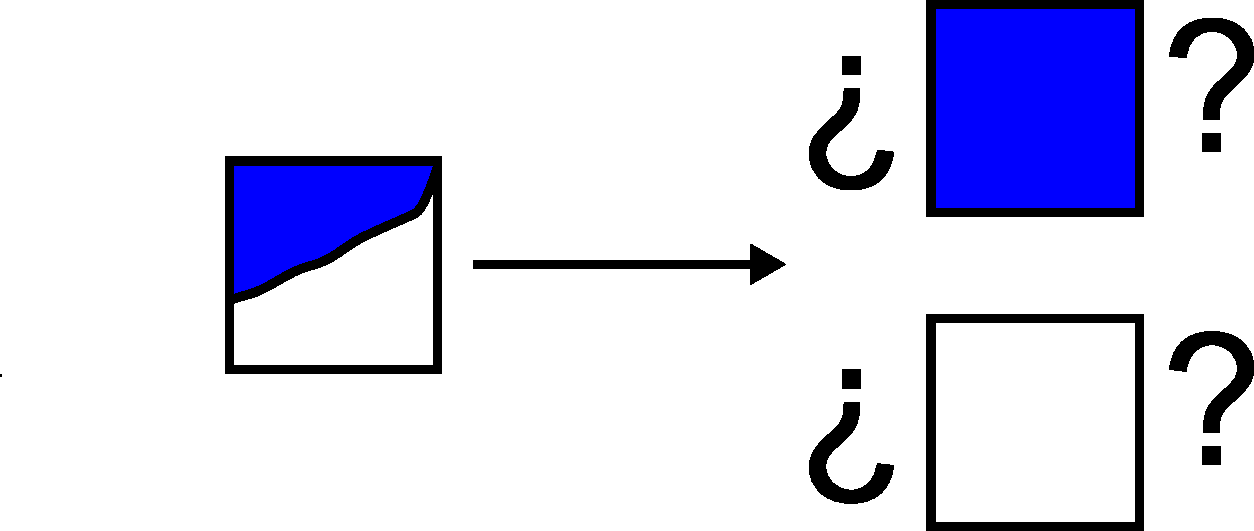
\includegraphics[width=.4\mycolumnwidth]{Tipos_datos/Ambiguedad_raster.pdf}
\caption{\small Ambig�edad en la asignaci�n de valores a una celda en una capa r�ster, debido al tama�o de esta, que condiciona la precisi�n con la que puede recogerse la realidad existente sobre el terreno.}
\label{Fig:Ambiguedad_raster} 
\end{figure}

Hay que tener en cuenta, no obstante, que la precisi�n de la representaci�n vectorial es, precisamente, de la representaci�n como tal, es decir, del modelo, pero no del dato en s� que tenemos en dicho formato vectorial, el cual depende de otros condicionantes tales como la escala de trabajo. Existe siempre incertidumbre en los datos, y el modelo de almacenamiento no excluye esta circunstancia. Los aspectos relativos a la calidad de los datos, tanto para datos r�ster como vectoriales, se desarrollan en profundidad en el cap�tulo \ref{Calidad_datos}.
\item Volumen de almacenamiento. El n�mero de elementos a almacenar es, en general, muy superior en el caso del modelo r�ster. Esto es as� debido a que toda la superficie a recoger se divide en las mismas unidades, independientemente de la complejidad de la variable en cada punto o de la necesidad de estudiarla con mayor o menor detalle en unos puntos que en otros. Para variables que se conciban mejor seg�n un modelo conceptual de entidades discretas, el modelo vectorial resulta m�s adecuado, ya que todas las zonas sin entidades no es necesario registrarlas de modo explicito, mientras que en el modelo r�ster estas deben registrarse de igual modo que aquellas en las que s� existe informaci�n relevante.
Los modelos de almacenamiento r�ster que veremos en el siguiente punto solucionan en parte el problema de los grandes vol�menes de datos del modelo r�ster, y son un elemento importante en la implementaci�n eficiente del mismo.
\item Complejidad. La regularidad y sistematicidad de las mallas r�ster hacen sencillo el implementar algoritmos de an�lisis, muy especialmente aquellos que implican el uso combinado de varias capas. Cuando estas capas est�n en formato r�ster y existe coincidencia entre sus mallas de celdas, el an�lisis conjunto de estas resulta inmediato. Por el contrario, la irregularidad espacial de las capas vectoriales hace que la implementaci�n de los mismos algoritmos sea sumamente m�s compleja si se trabaja con estas capas.

La sencillez de las capas r�ster, tanto en su concepto como en su implementaci�n, se ve apoyada adem�s por el hecho de que una capa r�ster se puede asemejar a una matriz, y por tanto aplicar sobre ella una serie de herramientas y elementos matem�ticos en muchos casos bien conocidos y de f�cil comprensi�n.

Existe de igual forma una distinta complejidad en t�rminos de proceso y c�lculo. Los algoritmos sobre una base r�ster pueden ser costosos en t�rminos de tiempo por la necesidad de aplicarlos sobre un n�mero muy elevado de celdas y un gran volumen de datos (v�ase el punto anterior). Por el contrario, los algoritmos sobre una base vectorial son costosos debido a que las operaciones matem�ticas que implican son m�s complejas y requieren mayores n�mero de c�lculos (aunque los vol�menes manejados puedan tambi�n ser notables).
\end{itemize}

Mas all� de las anteriores diferencias, a la hora de planificar un trabajo dentro de un SIG y elegir los datos que emplearemos y el modelo de representaci�n ideal, lo importante es entender que no existe un modelo de representaci�n id�neo de forma global, sino que esta idoneidad depende de muchos factores, como por ejemplo:

\begin{itemize}
 \item Tipo de variable o fen�meno a recoger. Como ya sabemos, algunas variables, en funci�n de su variabilidad y comportamiento espacial, son m�s adecuadas para el modelo vectorial, mientras que otras lo son para el modelo r�ster. Por ejemplo, en el caso de variables que requieran una intensidad de muestreo distinta seg�n la localizaci�n (variables que resulta interesante estudiar con m�s detalle en unos puntos que en otros) puede resultar m�s l�gico recogerlas de forma vectorial, pues el modelo r�ster implica una intensidad de muestreo constante a lo largo del �rea estudiada.
\item Tipo de an�lisis o tarea a realizar sobre dicha variable. El uso que demos a una capa tem�tica condiciona en gran medida el modelo de datos id�neo. Por ejemplo en el caso de una capa de elevaciones, su an�lisis se lleva mejor a cabo si esta informaci�n est� recogida seg�n el modelo r�ster. Sin embargo, si el objetivo principal es la visualizaci�n de esa elevaci�n en conjunto con otras variables, unas curvas de nivel pueden resultar m�s adecuadas, ya que, entre otras cosas, no interfieren tanto con otros elementos a la hora de dise�ar un mapa con todas esas variables.
\item Contexto de trabajo. Por ejemplo, si queremos trabajar con im�genes, esto nos condiciona al empleo de datos r�ster, ya que resulta mucho m�s sencillo combinarlos con las im�genes, las cuales siempre se presentan como capas r�ster. 
\end{itemize}

As�, en el desarrollo de un trabajo pueden aparecer circunstancias que hagan m�s adecuado utilizar el modelo r�ster y otras en las que el modelo vectorial sea m�s id�neo. En tal caso, deben combinarse ambas, pues es de esta forma como se obtendr�n mejores resultados. Un usuario de SIG no debe limitarse a trabajar de forma general con un �nico modelo de datos, con independencia del tipo de tarea que desempe�e, pues en cualquier caso ambos modelos de datos pueden aportar alguna ventaja.

Por �ltimo, es importante tener en cuenta que existen procedimientos para convertir entre los formatos r�ster y vectorial, de forma que el disponer de datos en un modelo de representaci�n particular no implica que debamos desarrollar nuestro trabajo sobre dichos datos directamente, sino que podemos efectuar previamente una conversi�n. Los cap�tulos \ref{Creacion_capas_raster} y \ref{Creacion_capas_vectoriales} tratan estos temas en profundidad.

\section{Modelos de almacenamiento}\label{Modelos_almacenamiento}

\index{Modelo!de almacenamiento}
Los modelos de almacenamiento son el ultimo escal�n en la cadena de etapas distintas que llevan desde la realidad existente al conjunto de simples valores num�ricos que almacenamos y manejamos en un SIG y que modelizan dicha realidad. Los modelos de representaci�n definen una forma de recoger la realidad mediante unidades b�sicas (sean estas celdas en una malla, o bien primitivas geom�tricas definidas de una u otra manera), mientras que los modelos de almacenamiento plantean b�sicamente un esquema de c�mo convertir dichas unidades en valores num�ricos de la forma m�s eficiente. Es decir, c�mo \emph{escribir} dichos valores en un soporte digital o guardarlos en la memoria del ordenador de la mejor manera posible.

Los modelos de almacenamiento deben atender principalmente a dos necesidades b�sicas, que son las que definir�n su idoneidad para cada tarea y tipo de dato:

\begin{itemize}
 \item Minimizar el espacio ocupado por los datos.
\item Maximizar la eficiencia de c�lculo.
\end{itemize}

La primera necesidad es especialmente importante, pues, como ya se ha dicho, los datos r�ster son con frecuencia muy voluminosos. Un modelo de representaci�n que minimice el tama�o de los datos, unido a un manejo �ptimo de memoria, son requisitos de suma importancia para todo SIG que maneje datos r�ster, m�xime considerando los grandes vol�menes de datos que hoy en d�a se manejan, tales como los correspondientes a im�genes de alta resoluci�n.

La necesidad de maximizar la eficiencia de c�lculo afecta principalmente a las representaciones vectoriales ya que en ellas las operaciones son complejas. La forma en que se estructuran los valores de cada entidad ha de minimizar el numero de accesos necesarios a estos, para de este modo obtener un mejor rendimiento en todas las operaciones de an�lisis.

\subsection{Modelos para representaciones r�ster}

El principal problema relativo al almacenamiento de capas r�ster se presenta para el conjunto de valores de las distintas celdas, que constituye la parte m�s voluminosa de la informaci�n recogida. Las coordenadas de las celdas de referencia o el tama�o de celda, por su escaso volumen, no conllevan dificultad alguna, y es en el almacenamiento de la malla de celdas en s� donde se encuentran las diferencias entre unos y otros modelos.

La forma m�s inmediata de almacenar una capa r�ster es simplemente almacenar sus valores uno a uno, en una estructura similar a la que la propia capa representa. Para el caso m�s habitual de capas con celdas cuadradas, sabemos que la malla de datos correspondiente se puede asimilar a una matriz, con las implicaciones que esto tiene a la hora de su manejo. As�, la forma m�s directa de recoger una malla de datos r�ster es mediante una matriz de datos. Esta forma de almacenamiento tiene las siguiente ventajas \cite{Egenhofer1991Maguire}:

\index{Matriz!de datos (modelo almacenamiento)}

\begin{itemize}
 \item Formato muy intuitivo. La mayor�a de desarrolladores est� familiarizado con el concepto de matriz y con las operaciones de calculo matricial que pueden aplicarse sobre estas.
\item Sencillez en la implementaci�n. Los lenguajes de programaci�n soportan sin problemas el uso de matrices bidimensionales y una serie de operaciones b�sicas sobre ellas.
\item Las mismas operaciones pueden aplicarse sobre todos los valores de la matriz de igual modo (todas las posiciones de la matriz son \emph{iguales} desde este punto de vista), lo que simplifica la implementaci�n de operaciones.
\item Resulta igualmente sencillo recorrer la matriz e iterar sobre la misma, lo cual refuerza lo anterior y simplifica a�n m�s la implementaci�n de todo tipo de procesos.
\end{itemize}

No obstante, el almacenamiento de todos los valores de forma id�ntica ignora el hecho de que pueden existir valores similares en zonas concretas, que pueden recogerse de formas mucho m�s �ptimas que una serie de n�meros iguales. En otras palabras, y de modo similar a como ocurre con el propio modelo de representaci�n r�ster, la estructura regular que confiere las ventajas es tambi�n la responsable de la mayor parte de los inconvenientes.

Como veremos en el cap�tulo \ref{Analisis_espacial}, las zonas pr�ximas entre s� (es decir, en el caso de una capa r�ster, las celdas pr�ximas entre s�), tienden a tener valores similares, en lo que se conoce como \emph{autocorrelaci�n espacial}. No considerar este hecho lleva al almacenamiento de informaci�n redundante, y ese es precisamente el principal problema del almacenamiento directo de una capa r�ster mediante una matriz. Almacenando expl�citamente todos los valores de la malla se desperdicia en muchos casos una gran cantidad de espacio (sea este en memoria, disco u otro soporte cualquiera).\index{Autocorrelaci�n espacial}

Podemos ver dos ejemplos claros de esto en las figuras \ref{Fig:Vias_modelos_representacion} y \ref{Fig:Malla_raster_rotada}. En la primera, existen �nicamente dos valores: los correspondientes a las celdas sobre las que se sit�a una v�a, o los correspondientes a las celdas donde estas no aparecen. Estos �ltimos ocupan la gran mayor parte de la capa, y lo hacen en bloque, de tal forma que almacen�ndolos individualmente se acaba teniendo una matriz de datos donde la practica totalidad de ellos son id�nticos. Como es f�cil de entender, este forma de proceder no es la m�s adecuada, al menos en t�rminos de volumen de almacenamiento.

En la segunda imagen, las zonas que aparecen como consecuencia de la rotaci�n de la imagen no contienen datos (esto es, contendr�n el valor arbitrario que codifica la falta de datos). Estas zonas tambi�n constituyen grandes bloques de celdas contiguas, con lo que el almacenamiento de todos los valores tambi�n es una soluci�n altamente redundante, especialmente en estas zonas fuera de la imagen como tal.

La soluci�n m�s habitual para considerar la redundancia de valores y lograr una compresi�n eficaz de los datos es la t�cnica denominada \emph{Run--Length Encoding}. \index{Run--Length Encoding}Esta t�cnica sencilla codifica una serie de $n$ valores id�nticos como un par de valores, el primero de los cuales representa el valor dicho que se repite $n$ veces, y el segundo es el n�mero de veces que se repite, esto es, $n$. 

As�, si la primera fila de la capa de v�as en formato r�ster no aparece ninguna celda de v�a, todas las celdas de dicha fila contendr�n el valor con que se codifica la ausencia de estas (sea, por ejemplo, el valor 0). El almacenamiento directo de todos los valores de la fila requerir�a tantos valores como columnas existan (sea $n$ el ancho de la fila), mientras que utilizando \emph{Run--Length Encoding}, bastar�a con almacenar el par (0, $n$).

A la hora de tratar el conjunto de todas las celdas, se define un orden en el que recorrerla, denominado \emph{orden de barrido} o \emph{de escaneo} (Figura \ref{Fig:Orden_escaneo}), de tal modo que la matriz bidimensional queda reducida a una cadena de valores, es decir, a un vector unidimensional. Los distintos \emph{trozos} de esa cadena se van codificando seg�n el esquema anterior, de tal modo que cuando aparecen muchos valores iguales consecutivos, estos pueden sustituirse ventajosamente por un �nico par de valores.\index{Orden!de barrido}\index{Orden!de escaneo}

\begin{figure}[!hbt]   
\centering
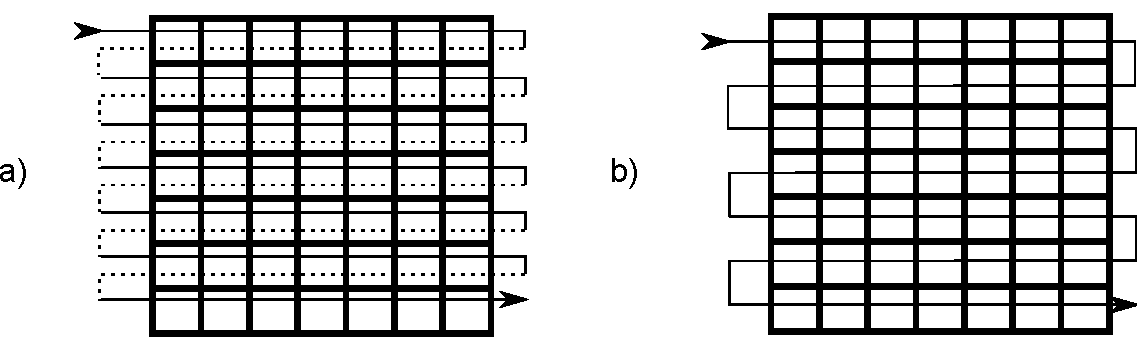
\includegraphics[width=.75\mycolumnwidth]{Tipos_datos/Ordenes_escaneo.pdf}
\caption{\small Ordenes de escaneo. a) fila a fila sin retorno, b) fila a fila con retorno.}
\label{Fig:Orden_escaneo} 
\end{figure}
 
La forma m�s sencilla de recorrer la imagen es hacerlo por filas, empezando por la fila superior y desplaz�ndose de derecha a izquierda (Figura \ref{Fig:Orden_escaneo}a). No obstante, el salto que se produce al final de cada fila suele implicar una discontinuidad en los valores. Invirtiendo la direcci�n del recorrido en cada fila, se tiene el orden mostrado en la figura \ref{Fig:Orden_escaneo}b, el cual suele tener como resultado mayores niveles de compresi�n de datos, ya que la cadena resultante de recorrer la imagen contiene \emph{trozos} generalmente de mayor tama�o.

Un esquema de barrido m�s complejo es el basado en el denominado \emph{orden de Morton} \cite{Morton1966IBM}. El orden de Morton (tambi�n conocido como \emph{orden Z}), se basa en una curva de car�cter recursivo, que recorre las celdas de la matriz siguiendo tramos en forma de Z, de ah� el nombre. En la primera iteraci�n se divide el conjunto de celdas en cuatro bloques, los cuales se recorren siguiendo el antedicho recorrido en Z. Si los bloques contienen a su vez m�s de una celda, se siguen subdividiendo a su vez de forma id�ntica, y as� hasta que no pueda continuarse este proceso.\index{Orden!Z}

La matriz que contiene los valores de orden de Morton (el orden en que se visita cada celda seg�n el esquema anterior, se conoce como \emph{Matriz de Morton}), la cual ya citamos por su importancia hist�rica en el cap�tulo \ref{Historia}\index{Matriz!de Morton}\index{Orden!de Morton}\index{Morton!matriz de}\index{Morton!orden de}

\begin{figure}[!hbt]   
\centering
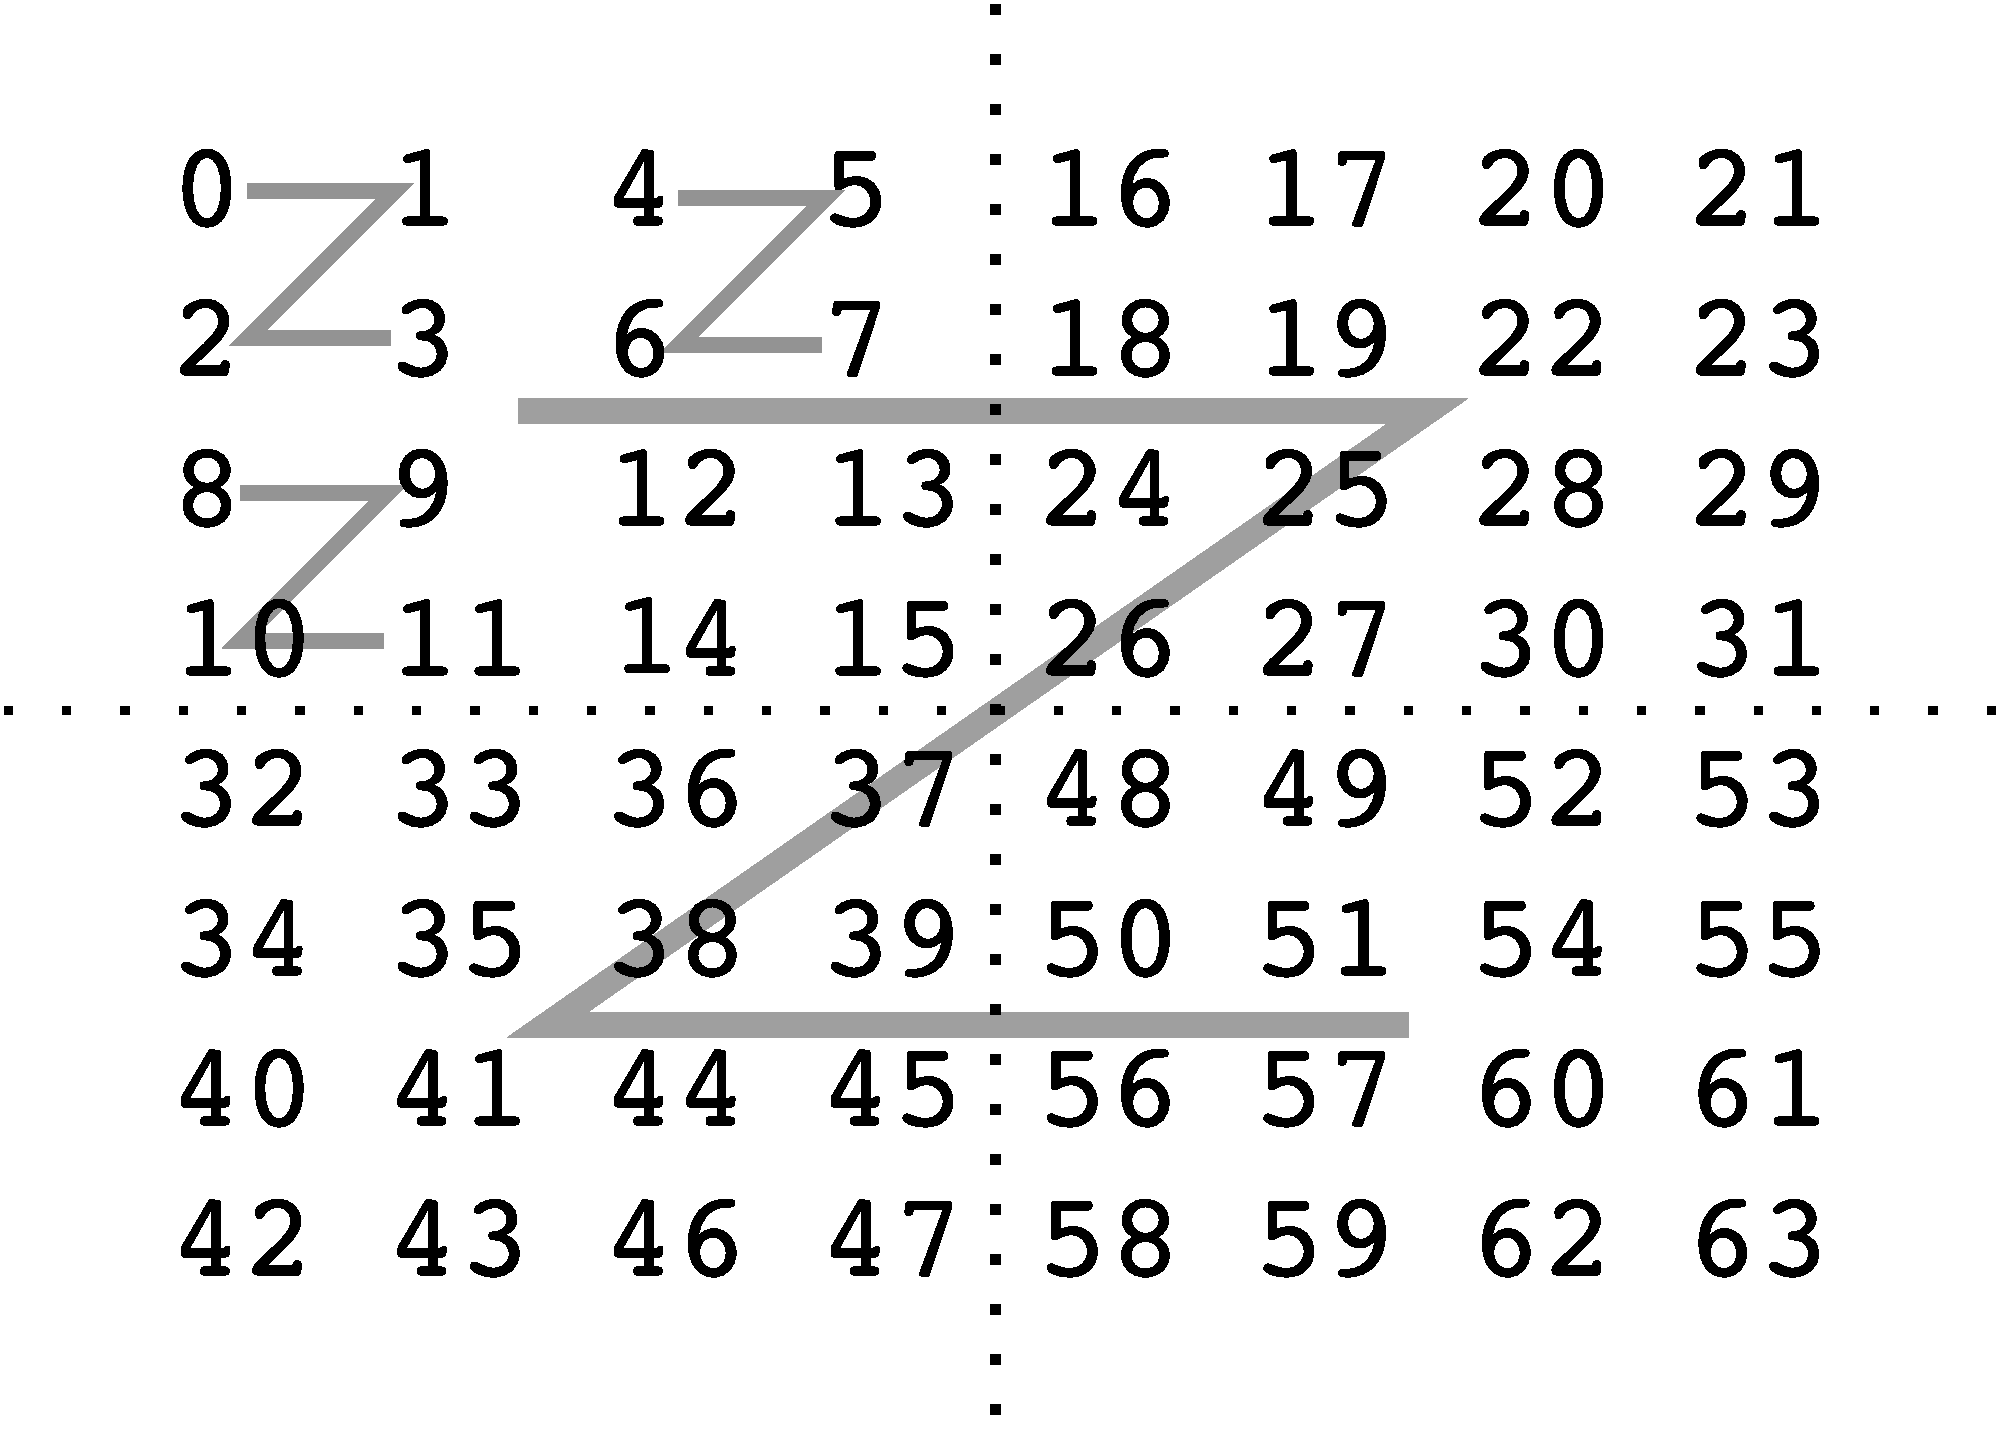
\includegraphics[width=.4\mycolumnwidth]{Tipos_datos/Orden_Morton.pdf}
\caption{\small Un ejemplo sencillo de barrido de una capa r�ster seg�n �rdenes de Morton. Los valores en las celdas no indican los valores de la variable, sino el orden en que se visita dicha celda seg�n este esquema de barrido}
\label{Fig:Orden_Morton} 
\end{figure}

Un ejemplo de este orden de barrido aplicado a una peque�a matriz puede verse en la figura \ref{Fig:Orden_Morton}.

Una estructura m�s avanzada son los denominados \emph{Quadtrees} o �rboles cuaternarios. Estas estructuras tambi�n dividen el espacio en cuadrantes sucesivamente, pero lo hacen con m�s profundidad en aquellas zonas que as� lo requieran por contener mayor n�mero de elementos y necesitar mayor resoluci�n. En el caso de una capa r�ster, se requerir� m�s detalle siempre que todas las celdas dentro de un cuadrante no tengan el mismo valor. En el caso m�s extremo, se ha de descender hasta el nivel de una sola celda, pero puede ser que un bloque de celdas contiguas tenga el mismo valor, en cuyo caso el cuadrante correspondiente las engloba a todas y las define con dicho �nico valor, sin necesidad de subdividirse m�s. De este modo, se adapta el modelo de almacenamiento a la propia estructura de la capa y al comportamiento que en esta muestra la variable estudiada.
\index{Quadtree}

Un ejemplo gr�fico de un �rbol cuaternario puede encontrarse en la figura \ref{Fig:Quadtree}. Los arboles cuaternarios son empleados tambi�n en los \emph{�ndices espaciales}, asociados a representaciones vectoriales, que veremos en \ref{Indices_espaciales} (de hecho, puede apreciarse que la figura anterior representa la aplicaci�n de un �rbol cuaternario a un conjunto de puntos, no a una capa r�ster, aunque el concepto es el mismo y su aplicaci�n a este segundo caso se realiza como ya se ha mencionado previamente).

Los quadtrees son estructuras complejas, y no profundizaremos m�s en su descripci�n dentro de este cap�tulo. Para el lector interesado, la definici�n original de esta estructura de datos puede encontrarse en \cite{Finkel1974Acta}. 

\begin{figure}[!hbt]   
\centering
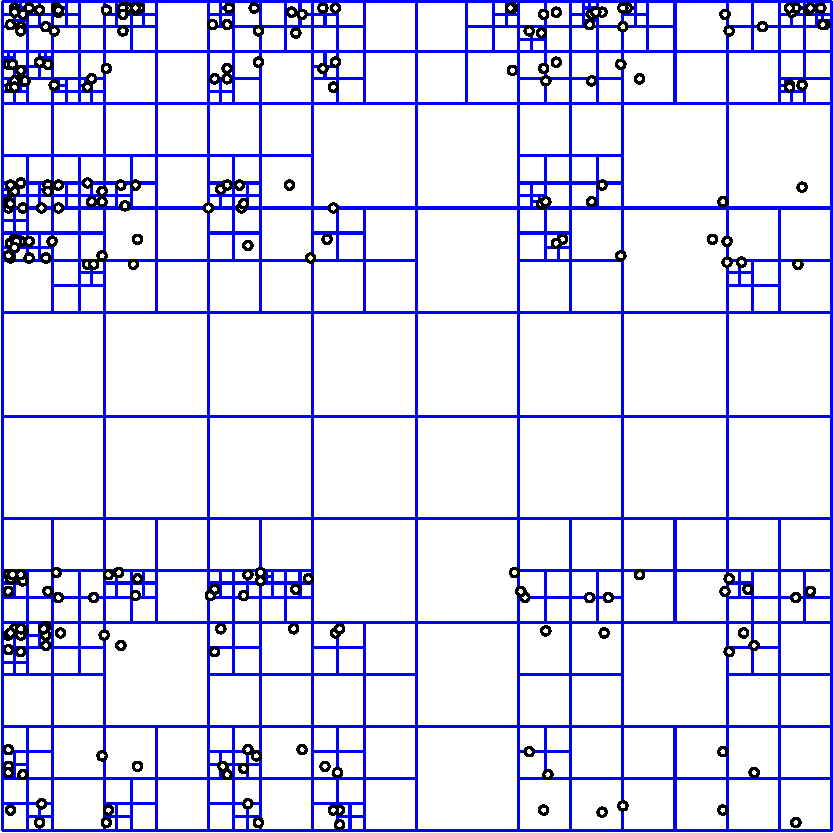
\includegraphics[width=.4\mycolumnwidth]{Tipos_datos/Quadtree.pdf}
\caption{\small Ejemplo de un �rbol cuaternario. En las zonas con m�s variabilidad (mayor densidad de puntos), los cuadrantes se subdividen hasta una profundidad mayor. La estructura es tal que cada cuadrante tiene dentro a lo sumo un punto. (Tomado de Wikipedia)}
\label{Fig:Quadtree} 
\end{figure}

Es importante rese�ar que cuando la capa r�ster contiene una informaci�n tal como una red viaria, la cual es susceptible de presentar valores id�nticos en celdas contiguas, la codificaci�n de tipo \emph{Run--Length} ---con cualquiera de los esquemas de barrido anteriores--- es ventajosa. Sin embargo, no lo es tanto cuando se trabaja con otro tipo de variables. 

En una capa con valores de elevaci�n, las celdas pr�ximas tendr�n valores parecidos pero no id�nticos, con lo que no podr� sacarse partido a esta forma de almacenamiento. M�s a�n, en estos casos el volumen ocupado por los datos no solo no disminuye, sino que aumenta. Es por ello que los SIG han de implementar igualmente la capacidad de poder trabajar con uno u otro modelo de almacenamiento seg�n los casos, bien sea por elecci�n directa del usuario o tom�ndose de forma autom�tica el que el propio sistema considere m�s adecuado en cada ocasi�n.

Aunque el mayor problema de las capas r�ster es su gran volumen, tambi�n existen diversas alternativas enfocadas a mejorar la velocidad de acceso a datos y el rendimiento de las operaciones sobre estas capas. Estas alternativas afectan a las im�genes con m�ltiples bandas, ya que estas, como dijimos, se recogen en un �nico fichero, en el cual se incorpora toda la informaci�n de las distintas bandas.\index{Bandas}

La forma en la que las bandas se tratan dentro del fichero y el modo en que se ordenan los p�xeles de las distintas bandas, ambas definen el esquema de almacenamiento, presentando cada uno de ellos una serie de ventajas de rendimiento en funci�n de la actividad principal que se vaya a desarrollar con la imagen. Tres son los esquemas principales:

\index{Band Sequential (BSQ)}
\index{Band Interleaved by Lines (BIL)}
\index{Band Interleaved by Pixel (BIP)}
\index{Pixel}

\begin{itemize}
	\item \extr{Band Sequential} (BSQ). Los valores se almacenan por bandas. Es decir, primero todos los p�xeles de la banda 1, despu�s los de la banda 2, y as� sucesivamente. Este tipo de esquema da prioridad a la componente espacial, ya que permite acceder r�pidamente a todo el espacio cubierto por una banda, puesto que los p�xeles de dicha banda se encuentran almacenados en posiciones contiguas.
	\item \extr{Band Interleaved by Pixel} (BIP). Los valores se almacenan ordenados por posiciones de p�xel. Es decir, primero se almacenan todos los valores correspondientes al p�xel (0, 0)\footnote{Es una terminolog�a habitual empezar a contar en cero en lugar de en uno las coordenadas fila/columna de una imagen} (en todas las bandas existentes), despu�s los correspondientes al (0,1)\footnote{Es habitual recorrer la imagen por filas, de forma que la coordenada (0,1) representa la primera fila y la segunda columna}, y as� sucesivamente.
	En caso de que lo que interese sea, para un p�xel dado, conocer toda la informaci�n disponible (su valor en todas las bandas), el esquema BIP es m�s ventajoso, ya que permite accesos r�pidos a este tipo de informaci�n, sin necesidad de <<saltar>> de un valor a otro como suceder�a en el caso del esquema BSQ. A nivel de acceso, se prima la informaci�n espectral sobre la espacial.
	\item \extr{Band Interleaved by Lines} (BIL). Es un esquema intermedio en el que se recogen los valores por filas. Esto es, primero la fila 1 de la banda 1, luego la de la banda 2, y as� sucesivamente. Posteriormente se recoge la fila 2 para todas las bandas, y de este modo hasta cubrir toda la imagen. Se trata de un esquema intermedio entre los anteriores, permitiendo un acceso r�pido tanto a la informaci�n espacial como a la informaci�n espectral de las bandas.
\end{itemize}

La figura \ref{Fig:Esquemas_almacenamiento_bandas} se muestra un ejemplo muy sencillo de los anteriores esquemas. Para una imagen de $2\times 2$ celdas y dos bandas, se recoge el orden en que se almacenar�a capa valor seg�n cada uno de dichos esquemas.

\begin{figure}[!hbt]   
\centering
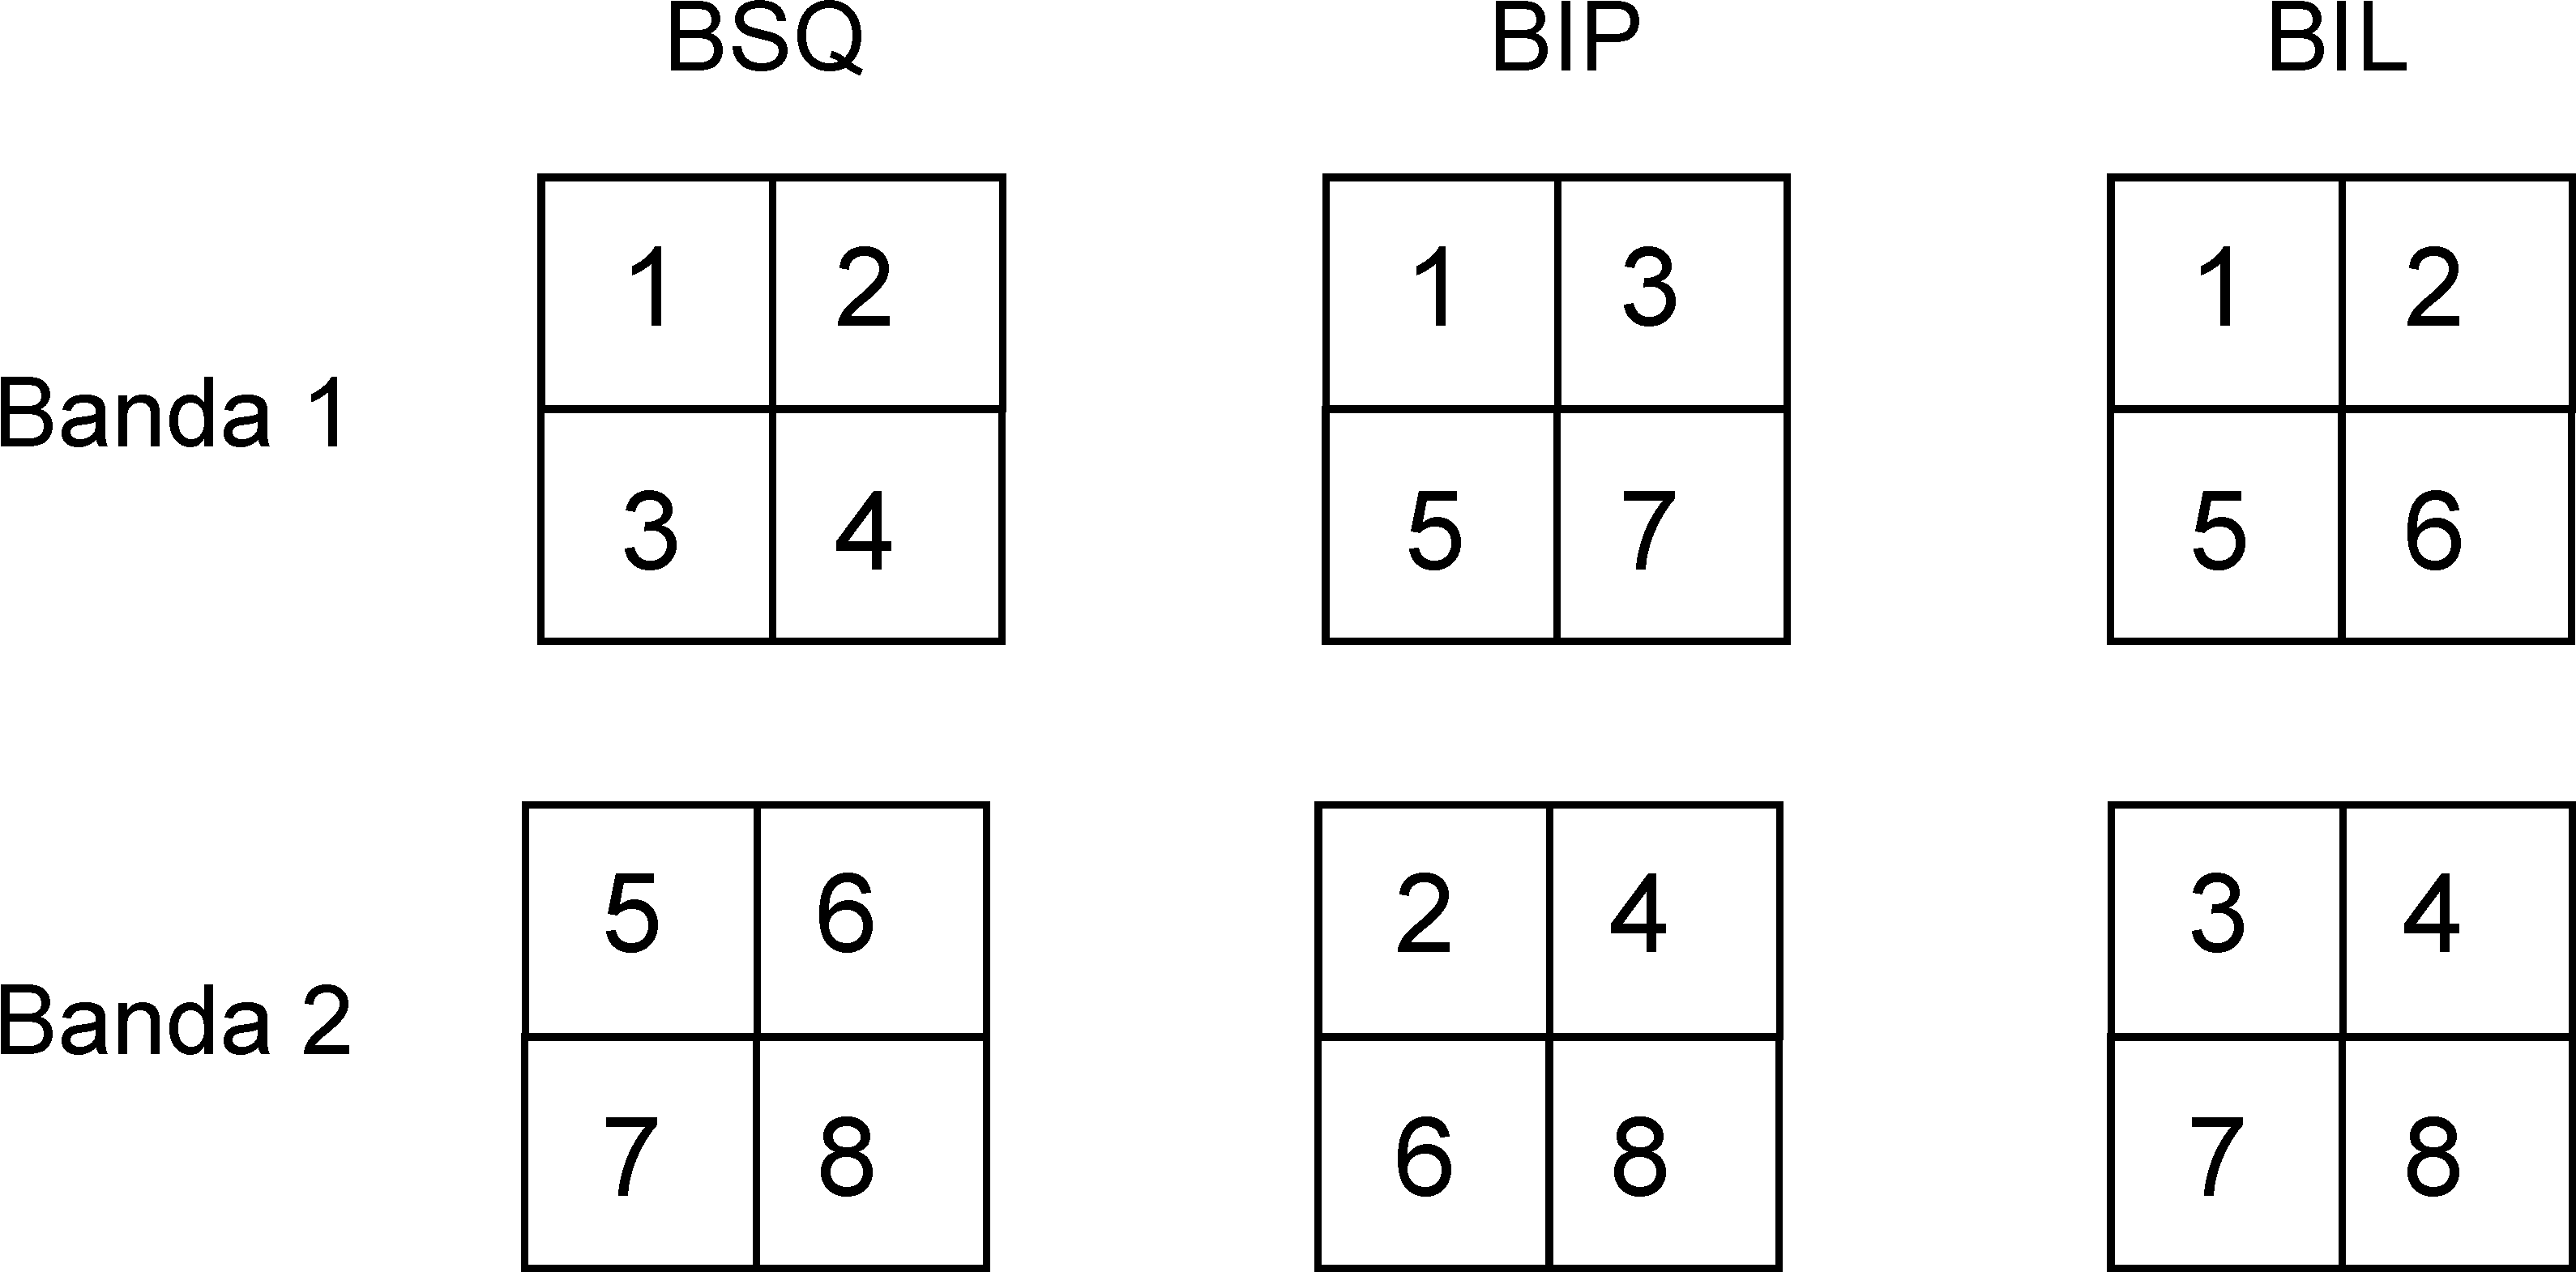
\includegraphics[width=.5\mycolumnwidth]{Tipos_datos/Esquemas_almacenamiento_bandas.pdf}
\caption{\small Esquemas de almacenamiento para im�genes multibanda. Los n�meros indican el orden en que se almacena cada valor.}
\label{Fig:Esquemas_almacenamiento_bandas} 
\end{figure}

\subsection{Modelos para representaciones vectoriales}

Al igual que para el modelo r�ster, existen para el modelos vectorial diferentes alternativas a la hora de almacenar los elementos que componen una capa. En realidad, ya hemos visto dentro de este cap�tulo algo que se asemeja a un modelo de almacenamiento, pues los modelo topol�gicos como DIME o el modelo \emph{arco--nodo}\index{Arco--nodo}, o los detallados para el caso particular de las redes, todos son en realidad esquemas de almacenamiento para el conjunto de \emph{piezas} que componen esa estructura topol�gica que se quiere almacenar. No obstante, tambi�n tienen algo de modelos de representaci�n, pues existe variaci�n en la forma en que conciben las partes de cada entidad (arcos entre dos nodos con o sin v�rtices intermedios, seg�n el modelo). 

En realidad, la raz�n por la que se han presentado en una secci�n anterior es porque de ese modo ayudaban a comprender mejor la existencia o no de topolog�a en una representaci�n, y ese aspecto resulta m�s importante para el estudio de los SIG que los modelos de almacenamiento. Estos, como se ha dicho, est�n a un nivel m�s bajo y alejado del usuario.

En general, los modelos de datos vectoriales no buscan tanto la disminuci�n de volumen de los datos como la obtenci�n de una mayor eficacia en las operaciones y una simplificaci�n de estas. L�gicamente, si los datos tienen un volumen menor, el tiempo que cualquier operaci�n sobre ellos implica tambi�n ser menor. A�n as�, la diferencia principal para este tipo de datos reside en la disminuci�n de la complejidad en que estos se almacenan, disminuyendo las operaciones a realizar, as� como la  complejidad de la implementaci�n de los correspondiente algoritmos (ambas habitualmente elevadas).

Para mejorar el rendimiento de las operaciones que trabajan con datos vectoriales, un factor clave es mejorar el acceso a los datos, de forma que, cuando se necesite acceder a unos datos concretos, estos puedan <<encontrarse>> de forma f�cil. Por este motivo, un elemento importante en la representaci�n de los datos vectoriales son los denominados \emph{�ndices espaciales}.\index{Indice@�ndice!espacial}

El concepto de �ndice cuando se habla de datos es similar al concepto de �ndice referido a un libro como este. Aqu� tienes un ejemplo muy sencillo para que lo comprendas mejor: si vas al principio de este libro, puedes ver su �ndice y saber d�nde empieza este cap�tulo, de forma que si estas interesado en modelos relacionados con la informaci�n geogr�fica, sabes r�pidamente que es en este bloque de p�ginas donde debes buscar lo que te interesa. Si no existiera ese �ndice, tendr�as que ir revisando todas las p�ginas hasta que llegaras al principio de cap�tulo y te dieras cuenta de que aqu� es donde est� lo que buscas. De igual modo, si vas al final de este libro y buscas el t�rmino \emph{�ndices espaciales}, ver�s que aparece esta p�gina junto con otras en las que aparece dicho t�rmino. Si no tuvieras ese �ndice, tendr�as que revisar palabra por palabra para saber en qu� partes de este libro se habla de �ndices espaciales.

Estos sencillos ejemplos muestran situaciones similares a las que aparecen en el uso habitual de un GIS, en las cuales trabajamos sobre una parte del total de los datos. Igual que buscamos un cap�tulo o un �nico t�rmino, podemos querer, por ejemplo, todas las entidades de una capa que est�n en una zona particular del espacio. Disponer de un �ndice acelera el proceso de localizar esas entidades que nos interesan. Por trabajar con informaci�n espacial, tales �ndices se denominan �ndices espaciales.

Muchos de los procesos que veremos en la parte \ref{Procesos} necesitan este tipo de �ndices para poder ejecutarse con un rendimiento adecuado. A medida que veamos estos procesos, se comprender� mejor por qu� la existencia de �ndices espaciales resulta necesaria e incluso imprescindible cuando disponemos de datos de gran volumen. En el cap�tulo \ref{Consultas} veremos informaci�n m�s detallada sobre la utilidad de los �ndices espaciales, ya que estos son vitales para la realizaci�n de consultas espaciales, que son tratadas en dicho cap�tulo.\index{Consultas}

Como ya hemos dicho, el objetivo de este tipo de estructuras para representar los datos espaciales no es disminuir el tama�o, sino mejorar el rendimiento de las operaciones sobre ellos. De hecho, y al contrario que en el caso de los modelos de representaci�n r�ster, en este caso no disminuye el espacio que ocupan los datos, sino todo lo contrario, ya que este aumenta. Un �ndice espacial es informaci�n adicional que incrementa la utilidad de dichos datos. Exactamente del mismo modo que el �ndice de este libro, que no sustituye al texto que ahora mismo estas leyendo, sino que se a�ade a este y te ayuda a manejarte a trav�s de �l y sacarle m�s partido.

La creaci�n del �ndice espacial supone la creaci�n de una estructura espacial en la cual se contienen objetos m�s simples que las propias entidades geom�tricas, estructuradas a su vez de forma tambi�n m�s sencilla que recogiendo sus coordenadas, y con un orden caracter�stico. Como hemos dicho, este �ndice espacial no sustituye al dato espacial, sino que lo complementa, optimizando la b�squeda de informaci�n dentro de este.

Existen dos enfoques principales para los �ndices espaciales: continuos y discretos \cite{Guting1994VLDB}. Los continuos utilizan las coordenadas mismas de las entidades, simplificando la forma de estas, mientras que en los discretos la simplificaci�n se aplica al espacio, discretizando este. En ambos, las entidades que se emplean son rectangulares en la mayor�a de los casos. La figura \ref{Fig:Tipos_indices_espaciales} muestra la aproximaci�n de una geometr�a poligonal que se obtiene en ambos tipos de modelos. 
\index{Indice@�ndice!espacial!tipos}

\begin{figure}[!hbt]   
\centering
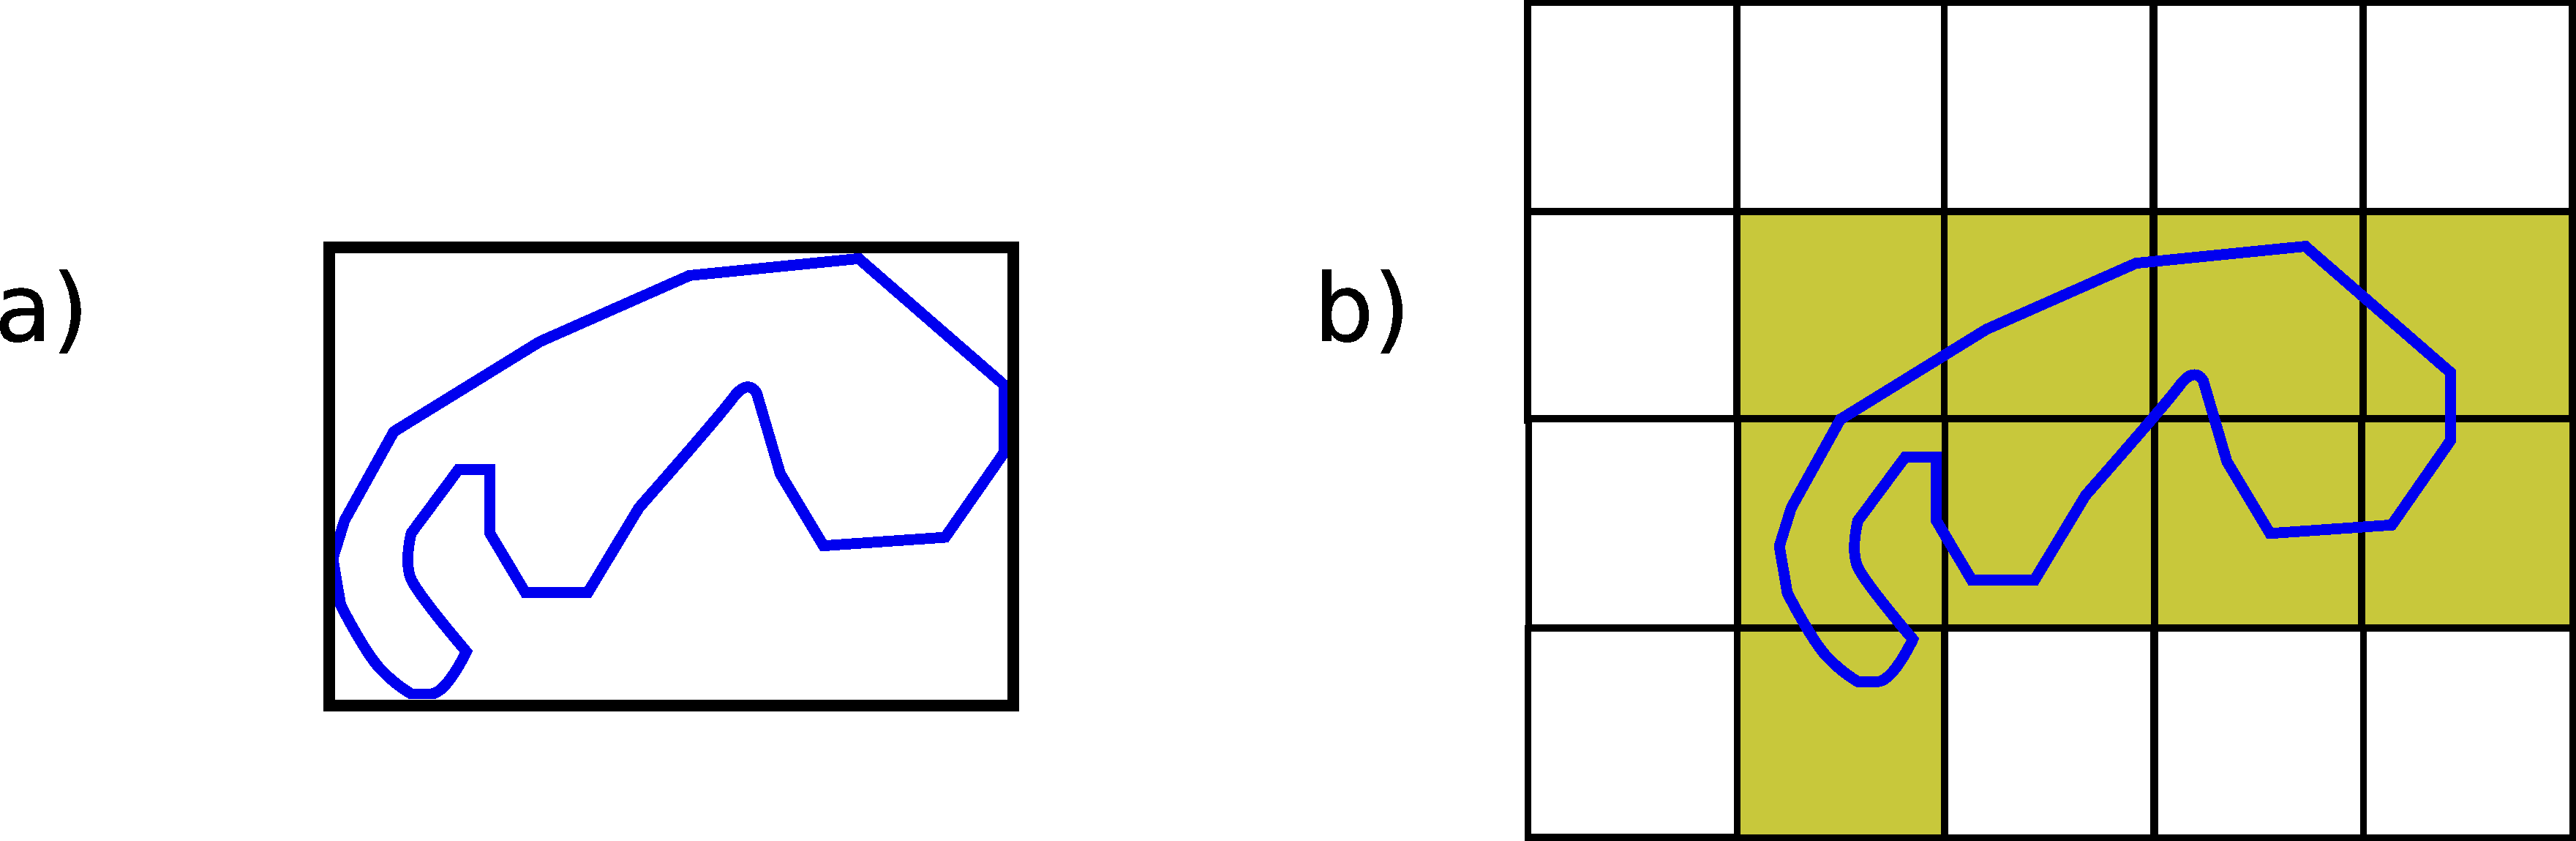
\includegraphics[width=.8\mycolumnwidth]{Tipos_datos/Tipos_indices_espaciales.pdf}
\caption{\small Aproximaci�n continua (a) y discreta (b) para un �ndice espacial.}
\label{Fig:Tipos_indices_espaciales} 
\end{figure}

En el caso continuo, se sustituye toda la complejidad del pol�gono por simplemente cuatro puntos: aquellos que conforman el rect�ngulo dentro del que este se inscribe. En el caso discreto, se reduce el pol�gono a unas cuantas celdas de una malla. Realizar comprobaciones sobre estas estructuras resulta mucho m�s sencillo, y por ello se emplean para realizar aproximaciones que simplifican las operaciones\footnote{Este proceso, conocido como \emph{filtrado y refinamiento}, lo veremos en detalle en el cap�tulo \ref{Consultas}}.\index{Filtrado y refinamiento}

Supongamos que utilizamos un �ndice espacial del primer tipo y queremos saber qu� pol�gonos de una capa se intersecan con otro dado. Para comprobar qu� pol�gonos se intersecan con este, en primer lugar podemos comprobar los solapes existentes entre sus rect�ngulos. Si los rect�ngulos no se solapan, es inmediato ver que los pol�gonos tampoco, con lo que no es necesario ya operar con ellos. Ver si dos rect�ngulos se solapan es casi inmediato, mientras que esta misma operaci�n para pol�gonos complejos requiere un numero mucho mayor de operaciones.

Debido al uso de rect�ngulos como elementos b�sicos, las estructuras que se emplean est�n espec�ficamente dise�adas para contener o bien rect�ngulos (en el caso de entidades de l�neas o de pol�gonos) o puntos (en el caso de entidades puntuales). Estas estructuras no son nuevas para nosotros, ya que hemos visto algunas de ellas en este mismo cap�tulo. Por ejemplo, para el caso de una aproximaci�n continua sobre una capa de puntos, los arboles cuaternarios (\emph{quadtrees}) son una estructura de datos adecuada. Esta aplicaci�n ya la vimos, de hecho, en la figura \ref{Fig:Quadtree}.

Como seguramente ya hayas advertido, los enfoques continuo y discreto se corresponden a primera vista con las ideas correspondientes a los modelos de datos r�ster y vectorial (aunque los �ndices espaciales de los que estamos hablando son para capas vectoriales). Es por ello que las estructuras que hemos visto para el almacenamiento de datos r�ster pueden utilizarse tambi�n para recoger las distintas celdas de un �ndice espacial discreto. As�, la divisi�n en celdas hace necesario un orden de escaneo\index{Orden!de escaneo}. El orden de Morton que ya conocemos se aplica en este caso, entre otros.\index{Orden!de Morton}

Una vez m�s, las estructuras de datos de todos estos �ndices espaciales suponen un elemento demasiado especifico para los contenidos de este libro, por lo que no se profundizar� en su teor�a. No obstante, estos son numerosos, ya que se trata de un �rea muy desarrollada. Referencias como \cite{Buchmann1990Springer} aportan descripciones m�s extensas para el lector interesado.

En caso de querer profundizar en los aspectos m�s t�cnicos de la representaci�n del dato geogr�fico en general, tanto en formato r�ster como vectorial, \cite{Worboys2004CRC} ofrece informaci�n muy extensa al respecto.

\section{Resumen}

El proceso de almacenar la realidad y reducirla a un conjunto de valores num�ricos manejables por un ordenador implica tres etapas fundamentales: creaci�n de un modelo conceptual, adopci�n de un modelo de representaci�n y codificaci�n del anterior seg�n un modelo de almacenamiento. Estos procesos dan lugar a la creaci�n de las denominada \emph{capas geogr�ficas}, unidades fundamentales de informaci�n dentro de un SIG.

Dos son los modelos conceptuales m�s importantes: campos y entidades discretas. Estos a su vez se identifican en l�neas generales con los dos principales modelos de representaci�n: r�ster y vectorial.

En el modelo r�ster el espacio se divide sistem�ticamente en unidades m�nimas denominadas celdas, habitualmente de forma cuadrada. En el modelo vectorial se almacenan las distintas entidades geogr�ficas a trav�s de las coordenadas de los puntos que las componen. El concepto de \emph{topolog�a} es importante en el modelo vectorial, y en funci�n de la forma en que se recojan las coordenadas de cada entidad, se almacenar� o no la informaci�n topol�gica. El modelo arco--nodo es el m�s habitual para representar la topolog�a.

La ultima etapa es la que conlleva el almacenamiento de los modelos de representaci�n, convirtiendo los elementos base de estos en valores num�ricos manejables por el ordenador. Cada modelo de representaci�n tiene sus particulares modelos de almacenamiento, los cuales tratan de maximizar el rendimiento de las operaciones realizadas sobre los datos espaciales, al tiempo que reducen el espacio que dichos datos ocupan.


\chapter{Fuentes principales de datos espaciales}\label{Fuentes_datos}

\begin{keypoints}
�Cu�les son los principales medios para obtener datos espaciales?$\bullet$�Qu� entendemos por fuente primaria y fuente secundaria de datos en un SIG?$\bullet$�En qu� principios se basan para recoger esos datos?$\bullet$�Qu� caracteriza a los datos recogidos mediante cada uno de estos medios?$\bullet$�Cu�les son sus usos m�s habituales?$\bullet$�C�mo se digitaliza un documento cartogr�fico impreso?$\bullet$�Cu�les son los fundamentos de la teledetecci�n y qu� productos cartogr�ficos genera?$\bullet$�Y del sistema GPS?
\end{keypoints} 

\bigskip

\begin{intro}
Una vez conocemos los modelos de representaci�n y sabemos c�mo almacenar la informaci�n geogr�fica, es momento de estudiar los distintos m�todos que nos permiten llevar a la pr�ctica el proceso de creaci�n del dato geogr�fico, y los or�genes desde los que estos se generan. En este cap�tulo analizaremos las principales fuentes existentes, sus fundamentos  y caracter�sticas, y c�mo son los datos que se obtienen a partir de ellas.

Para seguir el contenido de este cap�tulo, es importante tener una buena comprensi�n de todo lo descrito en el cap�tulo \ref{Tipos_datos}, en especial lo relativo a modelos de representaci�n.
\end{intro}

\section{Introducci�n}

El origen de los datos con los que trabajamos en un SIG puede ser sumamente variado y presentarse asimismo en formas diversas. La metodolog�a seguida en la recolecci�n de datos condiciona directamente la forma en que estos datos llegan a nosotros, y por tanto el uso que les podemos dar dentro de un SIG o las operaciones que debemos realizar con ellos de cara a poder adaptarlos para la realizaci�n de un trabajo concreto.

No hace tanto tiempo, toda la informaci�n que se manejaba dentro de un SIG ten�a su origen en un mapa en papel, el cual deb�a \emph{prepararse} para adaptarse a la naturaleza propia del SIG. El desarrollo de los SIG ya hab�a comenzado a dar sus frutos y se obten�an los primeros programas, pero eran necesarios datos para utilizarlos. Sin embargo, los datos geogr�ficos de los que se dispon�a no se encontraban en formato digital, por lo que no eran adecuados para su uso dentro de un SIG.

Una tarea b�sica en esos tiempos era la digitalizaci�n de cartograf�a\index{Digitalizaci�n}, es decir, convertir los datos geogr�ficos en formato impreso en datos en formato digital que un SIG pudiera manejar. La disponibilidad de datos digitales era baja, pero, como resulta l�gico pensar, s� que exist�a una gran cantidad de datos geogr�ficos en otros formatos tales como mapas, cartas de navegaci�n, fotograf�as a�reas, etc. La tecnolog�a ha ido avanzando y ya se producen datos directamente en formato digital, considerando espec�ficamente la existencia de los SIG como herramientas b�sicas de manejo de datos geogr�ficos. No obstante, los datos en formato impreso, as� como las t�cnicas que se emplearon en su creaci�n, siguen siendo v�lidas, y sirven igualmente para crear datos geogr�ficos que podemos emplear en un SIG.

Hoy en d�a, la situaci�n es bien distinta a la de aquellos primeros tiempos, y puede afirmarse que los or�genes a partir de los cuales se generan los datos geogr�ficos son muy diversos. Esto es as� porque aunan t�cnicas recientes y m�s adaptadas al entorno de los SIG con m�todos cl�sicos que, no obstante, no han perdido su vigencia y valor. En la actualidad, la recolecci�n de datos geogr�ficos es un �mbito complejo con muchas alternativas, las cuales deben integrarse dentro de un SIG para permitir que este despliegue todo su potencial sobre dichos datos. Todo este conjunto de t�cnicas de adquisici�n de datos conforman un amplio abanico de posibilidades de las cuales el usuario de SIG debe nutrirse para trabajar siempre en las mejores condiciones posibles, maximizando la precisi�n y alcance de su trabajo.

Integrar dentro del trabajo con un SIG todas las fuentes de datos disponibles es una tarea que requiere un conocimiento detallado de estas, con objeto de poder establecer la mejor manera de combinarlas, y elegir en cada caso la mejor opci�n de las disponibles. A lo largo de este cap�tulo veremos las principales t�cnicas existentes para la creaci�n de datos geograficos en un formato apto para su uso en un SIG, centr�ndonos en los pormenores de proceso y las particularidades de los datos generados en cada caso. Para ello, veremos todo el conjunto de fuentes de las cuales pueden provenir los datos con los que trabajamos en un SIG, desde las m�s modernas hasta las m�s antiguas, as� como las metodolog�as que permiten convertir las formas no digitales en datos aptos para su uso en dicho SIG. El objetivo es que, al final del cap�tulo, se conozcan con detalle todas las formas en las que los datos geogr�ficos pueden presentarse, se entiendan estas completamente con independencia de su origen, y se sepan utilizar y combinar todas las fuentes de datos, extrayendo lo mejor de cada una de ellas.

\section{Datos digitales y datos anal�gicos}\label{Datos_digitales_y_analogicos}

La principal diferencia que se presenta desde la aparici�n de los SIG es la necesidad de utilizar datos digitales. Un SIG implica una aplicaci�n inform�tica, y esta se alimenta en �ltima instancia exclusivamente de datos digitales. Esta es la raz�n por la que debemos alimentar nuestro SIG con una serie de valores num�ricos, y llegar a ellos a partir de la realidad que se pretende modelizar implica toda una serie de etapas, las cuales ya vimos con detalle en el cap�tulo \ref{Tipos_datos}

Gran parte de los datos geogr�ficos que se producen actualmente son en formato digital. Otros, a pesar de producirse hoy en d�a, no lo son directamente. Y junto a estos tenemos, como ya sabemos, todos los datos (que no son pocos) generados con anterioridad y que se presentan en diversas formas. Pero si deseamos trabajar con ellos en un SIG, de un modo u otro todos habr�n de acabar siendo digitales.

Los datos geogr�ficos digitales tienen una serie de ventajas frente a los anal�gicos (adem�s del mero hecho de que podemos incorporarlos a nuestro SIG), y suponen, como sucede en muchos otros campos, un salto cualitativo importante. Entender las ventajas frente a los datos anal�gicos ayuda a comprender un poco m�s la importancia de los SIG y la relevancia que cobran en el manejo de los datos geogr�ficos. Estas ventajas pueden resumirse en las siguientes:\index{Ventajas datos digitales}

\begin{itemize}
 \item Sencillez de actualizaci�n. La cartograf�a digital es editable, y esto simplifica enormemente la introducci�n cambios. Si en una capa con informaci�n catastral cambia la frontera de una parcela, basta modificar esta frontera. En un mapa anal�gico habr�a que rehacer todo el mapa y volver a imprimirse. 

Adem�s, y gracias a la divisi�n en capas, pueden actualizarse a distintos ritmos las distintas variables, pues son independientes y pueden modificarse por separado.

Haciendo una analog�a con el mundo editorial, pi�nsese en un diario impreso, con una �nica edici�n al d�a, en la que se ha de esperar al d�a siguiente para introducir todas las noticias que se vayan produciendo durante esa misma jornada. En su equivalente digital, la informaci�n se actualiza pr�cticamente en tiempo real, y podemos conocer las noticias mucho antes, pues es m�s sencillo actualizar esa p�gina que volver a poner la imprenta en marcha.

Es asimismo muy importante el hecho de que, gracias a los sistemas que centralizan el acceso a los datos, esta edici�n y actualizaci�n de datos pueden hacerla varias personas de modo concurrente. Esto no resulta posible en el caso de cartograf�a impresa, donde frecuentemente se encuentra el problema de que una cartograf�a de uso interno en una organizaci�n (por ejemplo, un ayuntamiento que guarda un inventario de su mobiliario urbano) ha sido editada por varias personas (el operario que sustituye un elemento de ese mobiliario luego lo registra en su inventario, y en un instante distinto otro operario puede a�adir en su propio mapa la localizaci�n de un nuevo elemento a�adido), siendo necesario despu�s unir todas las modificaciones, lo cual no siempre resulta sencillo o incluso posible. 

Si varias personas trabajan con cartograf�a impresa de una zona, cada una de ellas tendr� su propio mapa. Con la cartograf�a digital, todos pueden obtener la cartograf�a de un repositorio central, de tal modo que si la editan, est�n editando una �nica versi�n, y no es necesario despu�s poner en com�n todas sus aportaciones para crear una nueva cartograf�a actualizada.

\item Facilidad de distribuci�n. Resulta m�s sencillo y menos costoso distribuir cartograf�a digital que anal�gica, ya que esto se puede hacer r�pidamente por Internet, por ejemplo. Volviendo al ejemplo del diario, las noticias se actualizan y se ponen en Internet, de donde cada lector las descarga de inmediato. El diario impreso requiere una cadena de distribuci�n m�s costosa, desde la imprenta hasta el punto de venta.
\item Espacio de almacenamiento. Se generan actualmente ingentes vol�menes de datos que adem�s, y gracias a que son m�s f�ciles de actualizar, se producen con una frecuencia mucho mayor. No obstante, un soporte digital puede almacenar una enorme cantidad de estos ocupando una fracci�n del espacio f�sico. En un ordenador dotado de una buena capacidad de almacenamiento caben los contenidos de una cartoteca y los de la hemeroteca de ese diario del que hablamos. Las mismas cartoteca y hemeroteca en formato impreso requieren edificios enteros.
\item Facilidad y precisi�n de an�lisis. Como ya veremos en la parte correspondiente, el salto cualitativo que se da en el campo del an�lisis es enorme. Podemos hacer con los datos geogr�ficos digitales cosas que no eran posibles con los anal�gicos y, mejor a�n, podemos automatizar estos an�lisis. Asimismo, la precisi�n es mayor, ya que depende �nicamente de los datos y la precisi�n intr�nseca de estos, pero no de la operaci�n de an�lisis (pi�nsese en un mapa impreso y una serie de operarios midiendo la longitud de un r�o sobre �l. Es probable que lleguen a resultados similares pero no id�nticos. Con cartograf�a digital, cualquier operario, y en cualquier SIG ---suponiendo que implementan todos las mismas f�rmulas--- llegar�a al mismo resultado exacto).
\item Facilidad de mantenimiento. Aunque no se introduzcan modificaciones y no se actualicen los datos, el formato digital hace m�s f�cil su conservaci�n. La degradaci�n del soporte no degrada directamente el dato en s�, haci�ndole perder calidad. La degradaci�n del soporte anal�gico (el papel), s� que lo hace. Adem�s, los datos digitales pueden replicarse con suma facilidad, por lo que su persistencia est� garantizada en mayor medida y a un menor coste que la de los datos anal�gicos.
\end{itemize}

As� pues, disponemos para nuestro trabajo en nuestro SIG de datos anal�gicos y datos digitales, siendo estos �ltimos los que necesitamos en �ltima instancia, y que presentan las ventajas anteriormente descritas frente a los primeros. En las siguientes secciones, veremos con detalle todos los distintos tipos de datos geogr�ficos, tanto digitales como anal�gicos, la forma en que se obtienen, sus caracter�sticas, c�mo se incorporan a un SIG, y en general todo aquello que resulte de inter�s para una mejor comprensi�n y uso posterior de los mismos. 

\section{Fuentes primarias y fuentes secundarias}

Como hemos visto, algunos datos que utilizamos en un SIG son de tipo anal�gico, mientras que otros son de tipo digital. En algunos casos (generalmente en los anal�gicos), estos datos no han sido tomados pensando en su utilizaci�n en un SIG, y nos van a servir de base para obtener otros que s� pueden emplearse directamente dentro de un SIG. Por el contrario, existen otros datos que ya han sido recogidos considerando su utilizaci�n dentro de un Sistema de Informaci�n Geogr�fica, y la forma en la que se presentan ya es adecuada para incorporarlos en este y trabajar con ellos.

En base a lo anterior, se define una forma distinta de clasificar los datos espaciales con los que trabajamos en un SIG: datos primarios (o procedentes de una fuente primaria) y datos secundarios (o procedentes de una fuente secundaria) \cite{Jackson1991Longman}.

Los datos primarios son aquellos que podemos emplear en un SIG y que, en su forma original, ya son susceptibles de ser sometidos a las operaciones de manejo y an�lisis que incorporan los SIG. En este grupo encontramos las im�genes digitales o los datos obtenidos con GPS\index{GPS}, todos ellos recogidos ya en origen de forma adecuada para su empleo directo en un SIG.

Por su parte, los datos secundarios derivan de alg�n otro tipo de dato previo, el cual no es adecuado para su empleo en un SIG. Entre estos incluimos las versiones digitales de los mapas cl�sicos (veremos en breve c�mo se lleva a cabo esa conversi�n de un documento anal�gico a uno digital\index{Conversi�n!anal�gico--digital}), as� como los datos procedentes de un muestreo o levantamiento tradicional. Otros provenientes de cartograf�a impresa, tales como capas de elevaciones, tambi�n se incluyen en en este grupo.

Al desarrollar las fuentes de datos en este cap�tulo, se tratar�n tanto fuentes primarias como secundarias, y en el caso de estas �ltimas se tratar�n a su vez las formas en las que a partir de estas pueden derivarse datos digitales que puedan ya ser incorporados a un SIG.

\section{Teledetecci�n}\index{Teledetecci�n}

La primera fuente de datos que trataremos en este cap�tulo es la teledetecci�n. Entendemos por teledetecci�n el estudio y medida de las caracter�sticas de una serie de objetos (en nuestro caso elementos de la superficie terrestre) sin que exista contacto f�sico \cite{Curran1991Longman,Lillesand1997Wiley,Chuvieco1996Rialp}. Para ello, se miden las perturbaciones que el objeto provoca en su entorno, principalmente las de tipo electromagn�tico.

Tradicionalmente, la teledetecci�n se ha estudiado como una materia complementaria pero en cierto modo separada de los Sistemas de Informaci�n Geogr�fica. Ello es debido principalmente a que se trata de una materia muy extensa cuyo desarrollo se ha producido en cierta parte de forma ajena al de los SIG. No obstante, a medida que ambos campos se han ido desarrollando, la convergencia entre SIG y teledetecci�n se ha ido haciendo cada vez m�s evidente. No solo las aplicaciones SIG incorporan elementos para el manejo, tratamiento y an�lisis de datos procedentes de la teledetecci�n, sino que las formulaciones de ambos �mbitos contienen elementos similares.

La teledetecci�n es hoy en d�a un elemento clave para la formaci�n en SIG, y como tal debe incluirse en un libro como este. Los bloques tradicionales en los que se divide el temario fundamental de la teledetecci�n no incorporan �nicamente el registro de la informaci�n y la creaci�n de los datos, sino tambi�n su proceso posterior, interpretaci�n y tratamiento. Estos �ltimos no se tratan, sin embargo, en este cap�tulo, sino en la parte \ref{Procesos} dedicada a los procesos, integrados junto con otras formulaciones similares para proceso de im�genes.

La teledetecci�n es, como decimos, una fuente de datos primordial en los SIG, y el verdadero aprovechamiento de los productos actuales de la teledetecci�n solo se da con el concurso de los SIG y sus capacidades de an�lisis y manejo de datos. No obstante, y atendiendo a la definici�n dada, los procesos de teledetecci�n aplicados al �mbito cart�gr�fico y el an�lisis espacial se remontan a tiempo atr�s, concretamente a la mitad del siglo XIX. Fue entonces cuando se tomaron las primeras fotograf�as a�reas uniendo el reci�n desarrollado campo de la fotograf�a junto con la utilizaci�n de globos aerost�ticos como medio para situar el aparato fotogr�fico a una altura suficiente que permitiera obtener las im�genes.

Las fotograf�as a�reas fueron el primer producto de la teledetecci�n, pero hoy en d�a existen otros  que, basados en esa misma idea de registro de informaci�n, pueden ser empleados como fuentes de datos espaciales dentro de un SIG. Para comprenderlos, estudiemos algo m�s en detalle los elementos del proceso de teledetecci�n, los cuales se representan de forma esquem�tica en la figura \ref{Fig:Elementos_teledeteccion}. Estos elementos son los siguientes:

\begin{figure}[!hbt]   
\centering
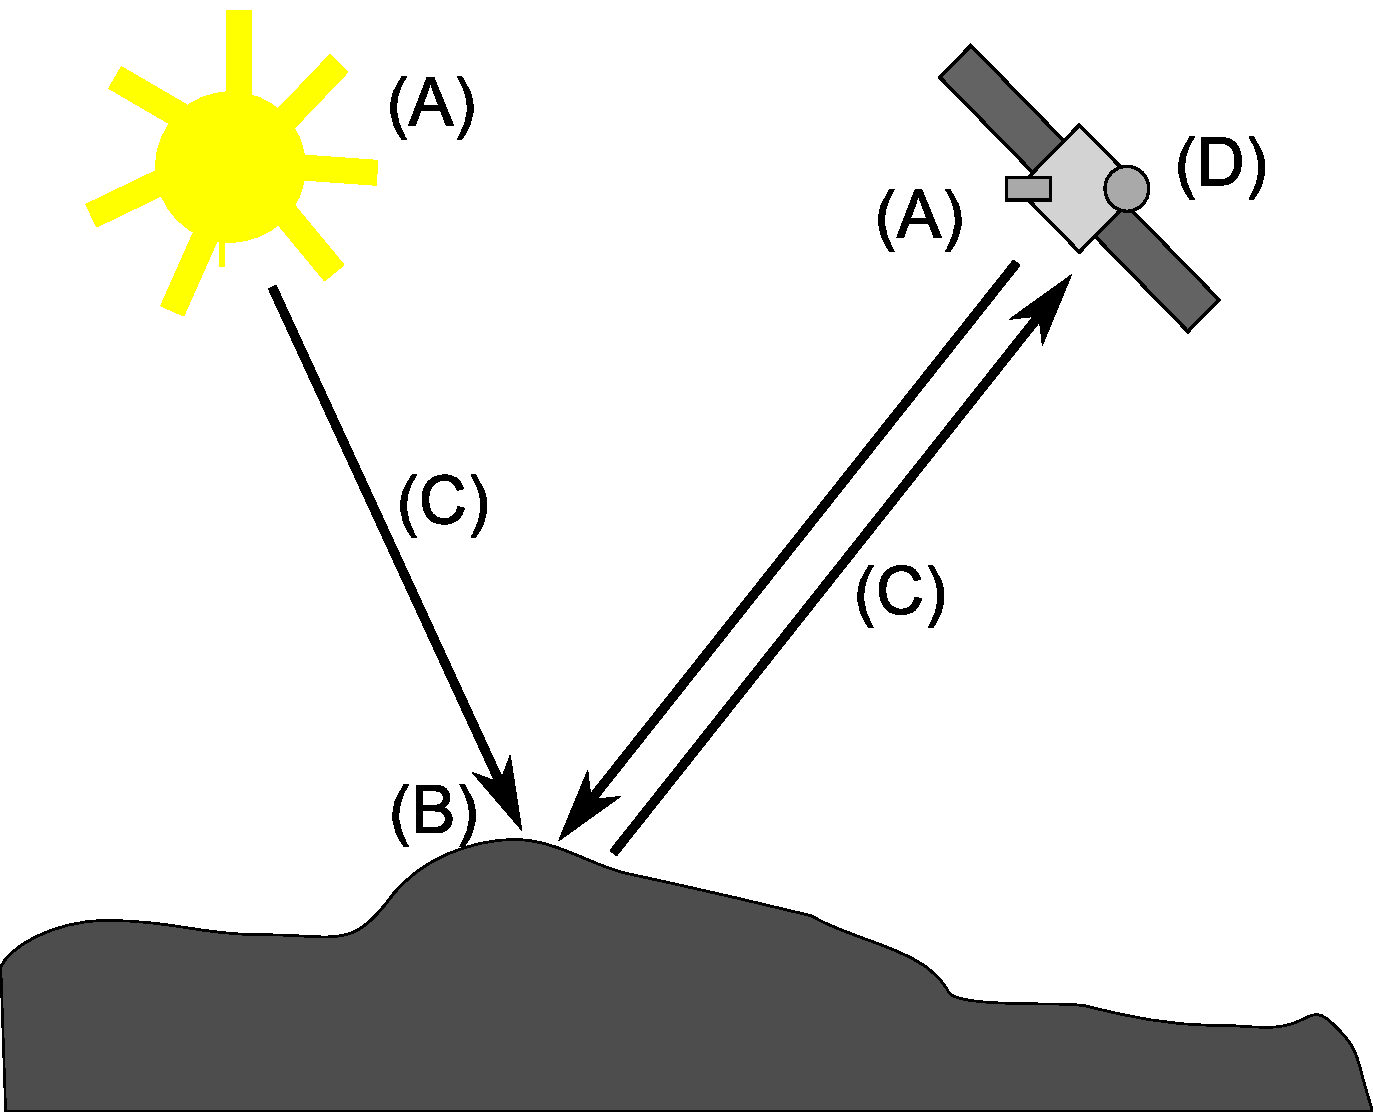
\includegraphics[width=.4\textwidth]{Fuentes_datos/Elementos_teledeteccion.pdf}
\caption{\small Esquema de un sistema de teledetecci�n.}
\label{Fig:Elementos_teledeteccion} 
\end{figure}

\index{Teledetecci�n!elementos}

\begin{itemize}
	\item Una fuente de radiaci�n (A)\index{Fuente de radiaci�n}. Puede ser de origen natural o artificial. La radiaci�n emitida por dicha fuente llega al terreno y sufre una perturbaci�n causada por los elementos de este, siendo esta perturbaci�n el objeto de estudio de la teledetecci�n. Los propios objetos pueden ser tambi�n emisores ellos mismos de radiaci�n.
	\item Unos objetos (B) que interaccionan con la radiaci�n o la emiten, seg�n lo anterior.
	\item Una atm�sfera (C) por la que se desplaza la radiaci�n, tanto desde la fuente hasta el objeto como desde el objeto hasta el receptor. La atm�sfera tambi�n interact�a con la radiaci�n, introduciendo igualmente perturbaciones en ella.
	\item Un receptor (D) que recoge la radiaci�n una vez esta ha sido perturbada o emitida por los objetos. El receptor va a generar como producto final una imagen (en t�rminos de un SIG, una capa r�ster), en cuyas celdas o p�xeles\index{Pixel} se va a contener un valor que indica la intensidad de la radiaci�n. Estos valores son valores enteros que indican el nivel de dicha radiaci�n dentro de una escala definida (habitualmente valores entre 1 y 256), y se conocen dentro del �mbito de la teledetecci�n como \emph{Niveles Digitales}\index{Niveles Digitales}.
\end{itemize}

A lo largo de este apartado veremos con detalle estos elementos. Para estudiar los dos primeros, estudiaremos los fundamentos f�sicos relativos a la radiaci�n y a la la interacci�n entre esta y la materia, mientras que para el estudio del sistema receptor analizaremos los elementos de este en dos componentes por separado: sensores y plataformas. 

La interacci�n de la atm�sfera interesa de cara a eliminar su efecto, ya que lo que resulta de inter�s en general son los objetos en la superficie terrestre, no la atm�sfera como tal. Eliminar esta influencia de la atm�sfera es parte de los procesos posteriores que se realizan con la imagen y que incluyen tambi�n, como se mencion� anteriormente, la interpretaci�n y otros procedimientos diversos sobre esta. Todos ellos no son tratados en este cap�tulo sino, tal y como se dijo, en un cap�tulo independiente dentro de la parte de procesos.

\subsection{Fundamentos f�sicos}

Es necesario conocer los conceptos fundamentales sobre la radiaci�n y su interacci�n con la materia (los objetos de la superficie terrestre) para poder entender c�mo, utilizando la radiaci�n de una fuente dada, se crea una imagen como resultado final en un proceso de teledetecci�n.

\subsubsection{La radiaci�n electromagn�tica}\index{Radiaci�n electromagn�tica}

La radiaci�n electromagn�tica es una de las cuatro fuerzas fundamentales de la naturaleza\footnote{las otras tres son la gravitatoria, la interacci�n nuclear d�bil y la interacci�n nuclear fuerte} y deriva del campo electromagn�tico, el cual es ejercido por las part�culas cargadas el�ctricamente. Para explicar esta existen dos modelos conocidos como \emph{modelo ondulatorio} y \emph{modelo de part�culas}. Seg�n el primero, que ser� en el que profundicemos algo m�s, la radiaci�n electromagn�tica es producto de las alteraciones en los campos el�ctrico y magn�tico, que generan dos ondas ortogonales entre s�, correspondientes a cada uno de los campos anteriores (Figura \ref{Fig:Radiacion_electromagnetica}).\index{Modelo!ondulatorio}\index{Modelo!de part�culas}

\begin{figure}[!hbt]   
\centering
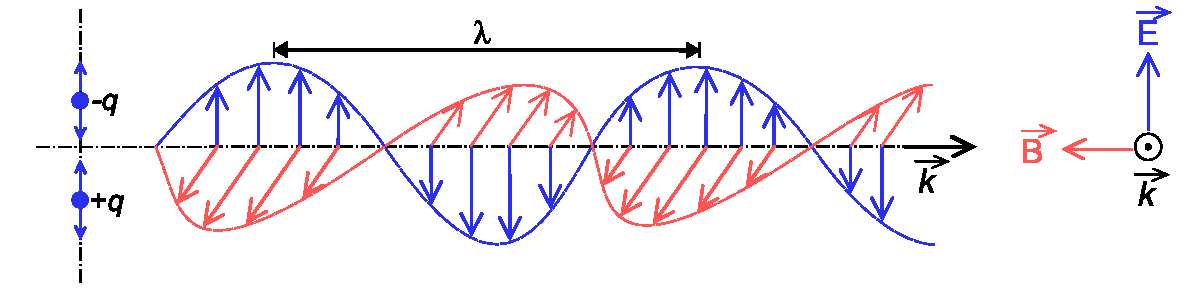
\includegraphics[width=.6\textwidth]{Fuentes_datos/Onde_electromagnetique.pdf}
\caption{\small Ondas correspondientes a los campos magn�tico y el�ctrico, ortogonales entre s� (Tomado de Wikipedia). }
\label{Fig:Radiacion_electromagnetica} 
\end{figure}

Estas ondas se desplazan a a la velocidad de la luz, y se pueden describir con los par�metros habituales, tales como la longitud de onda o la frecuencia\footnote{Se supone que el lector tiene cierta familiaridad con estos conceptos f�sicos b�sicos. En caso contrario, una referencia que puede encontrarse en la red es \cite{webbookOndas}}. Una mayor longitud de onda (y, por tanto una menor frecuencia) tiene asociada una mayor energ�a de la radiaci�n.\index{Longitud!de onda}

La radiaci�n electromagn�tica puede cubrir de forma continua todo un amplio rango de valores de longitudes de onda. Este rango se conoce como \emph{espectro electromagn�tico}\index{Espectro electromagn�tico}. Pese a la continuidad de sus valores, es habitual agruparlos en regiones, discretizando la amplitud del espectro, ya que las radiaciones en longitudes de onda similares presentan a su vez comportamientos similares en muchos sentidos. En la figura \ref{Fig:Espectro_electromagnetico} se muestra un esquema del espectro electrom�gn�tico y sus principales regiones de inter�s.

\begin{figure}[!hbt]   
\centering
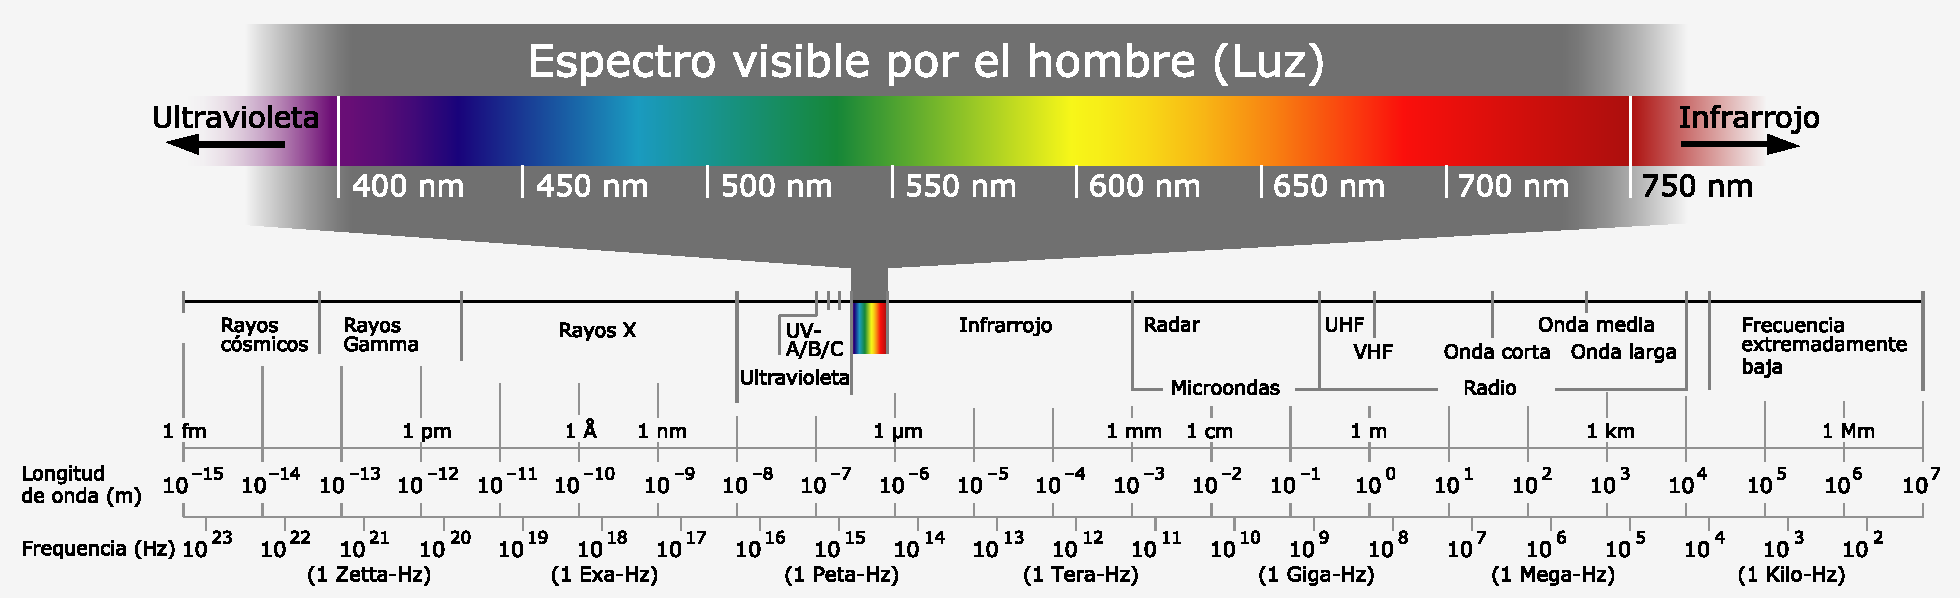
\includegraphics[width=\textwidth]{Fuentes_datos/Electromagnetic_spectrum-es.pdf}
\caption{\small Espectro electromagn�tico y sus principales regiones de inter�s (Tomado de Wikipedia).}
\label{Fig:Espectro_electromagnetico} 
\end{figure}

Dentro de estas regiones, son de destacar las siguientes:

\begin{itemize}
	\item Rayos $\gamma$  $<$0.03 $nm$.
	\item Rayos X (0.03 $nm$ - 3 $nm$).
	\item Ultravioleta (3 $nm$ - 0.3 $\mu$).
	\item Visible (0.3 $\mu$ - 0.7 $\mu$). Se corresponde con las radiaciones que pueden ser detectadas por el ojo humano o por aparatos tales como una c�mara fotogr�fica com�n. Observando la figura \ref{Fig:Espectro_electromagnetico} puede apreciarse que esta regi�n representa una porci�n muy peque�a del total del espectro. Existen muchas otras regiones que no podemos <<ver>> pero que, empleando la tecnolog�a adecuada, s� que pueden aprovecharse para crear im�genes dentro de un proceso de teledetecci�n, siendo de gran utilidad para el estudio de numerosos procesos.

\index{Rayos!X}\index{Rayos!gamma}\index{Regi�n!visible del espectro}\index{Regi�n!ultravioleta}

	Las distintas longitudes de onda dentro de esta regi�n son las responsables de los distintos colores que percibimos. As�, por ejemplo, el azul se corresponde con el rango entre 0.4 $\mu$ y 0.5 $\mu$, mientras que el verde lo hace con el rango entre 0.5 $\mu$ y 0.6 $\mu$
	\item Infrarrojo cercano (0.7 $\mu$ - 1.3 $\mu$).
	\item Infrarrojo medio  (1.3 $\mu$ - 8 $\mu$).
	\item Infrarrojo lejano o t�rmico (8 $\mu$ - 14 $\mu$). Dentro de esta regi�n se encuentran principalmente las radiaciones emitidas por los cuerpos debido a su temperatura\footnote{Esta emisi�n se calcula seg�n la denominada \emph{ley de Stefan--Boltzmann}. Puede encontrarse m�s al respecto en \cite{webSBoltzman}}.
	\item Microondas (1 $mm$ - 25 $cm$).
\end{itemize}

\index{Regi�n!infrarroja}\index{Microondas}

En el cap�tulo \ref{Procesado_imagenes} estudiaremos para qu� tipo de an�lisis resulta �til cada una de las regiones del espectro, cuando veamos como analizar las im�genes procedentes de la teledetecci�n.

Como ya se dijo en el cap�tulo \ref{Tipos_datos}, las im�genes como capas r�ster presentan habitualmente la particularidad de tener varias bandas\index{Bandas}. En lugar de un �nico valor para cada celda, existen $n$ valores, uno por cada banda. Esto es as� porque la imagen recoge la intensidad de la radiaci�n (recordemos que esto se denominaba Nivel Digital) dentro de una amplitud dada del espectro, y a su vez subdivide esta en distintas franjas. Los Niveles Digitales de cada banda corresponden a la intensidad dentro de una de esas franjas del espectro en particular.

\subsubsection{Interacci�n entre radiaci�n y materia}

La radiaci�n emitida por una fuente de radiaci�n es alterada por la presencia de los distintos objetos, que interact�an con ella. Independientemente de su procedencia, para toda radiaci�n se dan tres fen�menos fundamentales al alcanzar un objeto:

\begin{itemize}
	\item Absorci�n. El objeto toma la energ�a de la radiaci�n.
	\item Transmisi�n. La radiaci�n atraviesa el objeto y continua su camino.
	\item Reflexi�n. la radiaci�n <<rebota>> en el objeto y vuelve al espacio.	
\end{itemize}

\index{Absorci�n}\index{Tansmisi�n}\index{Reflexi�n}

Estos tres fen�menos se dan en diferente proporci�n en funci�n de las caracter�sticas del objeto y de la radiaci�n. Para una longitud de onda dada, existe, pues, un porcentaje de la radiaci�n que es absorbida por el objeto, otra que se transmite a trav�s de �l y otra que es reflejada. La parte que  interesa a efectos de la teledetecci�n es aquella que se refleja en el objeto, ya que esta es la que posteriormente puede recogerse y emplearse para la generaci�n de las im�genes.

La proporci�n en la que los tres procesos anteriores se dan en un objeto no es la misma para todas las radiaciones. Un objeto puede absorber una gran parte de la radiaci�n dentro de una regi�n del espectro y sin embargo reflejar la mayor�a de ella en una regi�n distinta. Es por ello que, en funci�n del an�lisis que se desee realizar, debe trabajarse con im�genes que traten una u otra regi�n.

Igualmente, una imagen con varias bandas contiene informaci�n sobre la intensidad de la radiaci�n reflejada en distintas partes del espectro. Puesto que cada objeto refleja de forma diferente la radiaci�n en cada una de esas partes, pueden igualmente emplearse para identificar objetos particulares si se conoce la respuesta de estos en determinadas bandas. Por ejemplo, si sabemos que los objetos que buscamos reflejan gran cantidad de radiaci�n en todas las longitudes de onda excepto en un rango concreto. Aparece as� el concepto de \emph{firma espectral} como la respuesta caracter�stica de un tipo de objeto dentro del espectro electromagn�tico. Veremos mucho m�s al respecto en el cap�tulo \ref{Procesado_imagenes}, as� como en el \ref{Estadistica_avanzada}, donde estudiaremos una aplicaci�n habitual de dichas firmas espectrales.\index{Firma espectral}

Adem�s de la interacci�n con los objetos que se pretenden estudiar, la radiaci�n interact�a con la atm�sfera. Esta interacci�n afecta al resultado y es una variable a considerar en ciertas operaciones posteriores con las im�genes. Veremos m�s sobre la interacci�n entre radiaci�n y atm�sfera en el apartado \ref{Correccion_imagenes}, cuando tratemos esas operaciones.

\subsection{Sensores y plataformas}

En un sistema de teledetecci�n, dos son los elementos tecnol�gicos principales que lo definen: el \emph{sensor} y la \emph{plataforma}. \index{Sensor}\index{Plataforma}

El sensor es el elemento que incorpora la capacidad de <<leer>> la radiaci�n electromagn�tica y registrar su intensidad dentro de la una zona concreta del espectro. En palabras m�s sencillas, es el aparato que nos permite <<tomar>> la imagen, y puede ir desde una simple c�mara fotogr�fica hasta un sensor m�s especializado capaz de tomar cientos de bandas en una regi�n del espectro de gran amplitud.

La plataforma, por su parte, es el medio en el que se sit�a el sensor y desde el cual se realiza la observaci�n. Los dos tipos principales de plataformas son aquellas situadas dentro de la atm�sfera terrestre (aviones en su mayor�a, aunque tambi�n en otros medios tales como globos aerost�ticos) y aquellas situadas fuera de la atm�sfera (a bordo de sat�lites)

Las caracter�sticas de estos dos elementos definen las del sistema en su conjunto, as� como las propiedades de sus productos derivados y la utilidad que estos presentan.

\subsubsection{Plataformas}

La plataforma es el medio en el que se transporta el sensor, y condiciona las mediciones efectuadas por este, ya que establece la distancia a la que el sensor se sit�a del elemento registrado (la superficie terrestre). Esta distancia puede ser del orden de algunos centenares de metros o unos pocos kil�metros, o bien de muchos kil�metros. En el primer caso, la plataforma m�s habitual es el avi�n, mientras que en el segundo caso lo m�s frecuente es el uso de sat�lites.

Los aviones son las plataformas cl�sicas a bordo de las cuales se montaban originariamente las c�maras empleadas para la realizaci�n de fotograf�as a�reas. No obstante, hoy en d�a pueden montarse igualmente otros sensores m�s complejos y modernos a bordo de aeronaves. 

Las ventajas del empleo de aviones como plataformas de teledetecci�n son las relacionadas con la disponibilidad de la plataforma, que es mucho mayor que en el caso de emplear sat�lites. Podemos (dentro de lo razonable) escoger c�mo, cu�ndo y d�nde efectuar un vuelo y tomar im�genes, mientras que en caso de sat�lites la disponibilidad viene condicionada por numerosos factores y es muy reducida.

Respecto a los inconvenientes, pueden citarse entre ellos la inestabilidad de la plataforma y la dependencia de las condiciones del clima, que pueden afectar a la propia estabilidad y a la calidad de los resultados, o incluso impedir la realizaci�n del vuelo. Por ser plataformas de baja altura, no pueden abarcar superficies tan amplias como los sat�lites, requiriendo m�s tiempo para cubrir una zona dada.

Por su parte, los sat�lites artificiales presentan unas caracter�sticas distintas como plataformas de teledetecci�n, siendo muy �tiles para la teledetecci�n sobre la superficie terrestre. Es habitual que a bordo de un mismo sat�lite coexistan diversos sensores, de forma que una �nica plataforma transporta varios de ellos.

A diferencia de un avi�n, un sat�lite no puede dirigirse a voluntad (no puede pilotarse), y su movimiento es una caracter�stica inherente que viene definida por una serie de par�metros. Estos par�metros se conocen como \emph{par�metros orbitales} pues definen la �rbita descrita por el sat�lite en torno a la Tierra. \index{Par�metros orbitales}\index{Orbita@�rbita}

Por una lado, las �rbitas pueden clasificarse en funci�n de su eje de rotaci�n en tres tipos:

\begin{itemize}
	\item Ecuatoriales, si se sit�an en el mismo plano en el ecuador terrestre.
	\item Polares, si se sit�an en un plano que contiene al eje de rotaci�n terrestre.
	\item Semipolares, si la �rbita es oblicua al eje de rotaci�n
\end{itemize}

Atendiendo a la forma en que se produce el movimiento, distinguimos dos tipos:

\begin{itemize}
	\item Geos�ncronas. El sat�lite se sit�a sobre un punto fijo de la Tierra y su movimiento sigue al de rotaci�n de esta. Es decir, no existe movimiento relativo entre dicho punto de la superficie terrestre y el sat�lite. Todas las im�genes que se toman desde el sat�lite tendr�n as� el mismo encuadre y cubrir�n una extensi�n id�ntica. La altura del sat�lite es fija, siendo esta de 35.786 Km, ya que esta altura hace que la velocidad del sat�lite se corresponda con la de rotaci�n de la Tierra.
	
	\index{Orbita@�rbita!Geos�ncrona}
	
	La ventaja de este tipo de sat�lites es que, por situarse siempre sobre un punto y siempre teniendo visi�n sobre una zona dada, se pueden actualizar con mucha frecuencia las im�genes. El inconveniente principal radica en el hecho de que las zonas alejadas del punto sobre el que se sit�a el sat�lite tendr�n mala cobertura, y existir�n zonas no cubiertas de las que no resultar� posible obtener im�genes con los sensores montados a bordo de dicho sat�lite. Pese a que un sensor sobre un sat�lite con �rbita geos�ncrona cubrir� una gran porci�n de la superficie terrestre (debido a la elevada altura a la que ha de situarse para tener dicha �rbita), no resulta posible, como es l�gico, cubrir toda ella y hacerlo adem�s en las mismas condiciones en todas las zonas.
	
	\item Helios�ncronas. Las �rbitas helios�ncronas son generalmente polares. Mientras el sat�lite recorre la �rbita, la Tierra efect�a su movimiento de rotaci�n, lo cual hace que a cada vuelta de la �rbita se cubran zonas distintas. De esta forma, se consigue dividir la totalidad de la superficie terrestre en bandas que se van recorriendo sucesivamente hasta que el sat�lite vuelve a situarse en el mismo punto inicial. Las �rbitas est�n dise�adas de tal manera que ese regreso al punto inicial se produce a la misma hora solar exacta que en el anterior ciclo, de forma que las im�genes tomadas en un punto dado son registradas siempre a la misma hora y en condiciones similares de iluminaci�n. Para que sea posible realizar una �rbita de este tipo, el sat�lite debe situarse entre 300 y 1500 Km de altura.
	
	La figura \ref{Fig:Orbita_landsat} muestra un ejemplo de la forma en que un sat�lite con una �rbita helios�ncrona barre toda la superficie de la Tierra.
	
	\index{Orbita@�rbita!Helios�ncrona}
	
\begin{figure}[!hbt]   
\centering
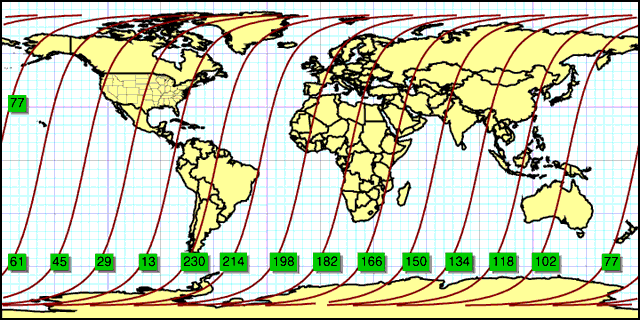
\includegraphics[width=.8\textwidth]{Fuentes_datos/Orbita_landsat.png}
\caption{\small Esquema de barrido de un sat�lite con �rbita helios�ncrona. Tomado de \cite{webLandsat}}
\label{Fig:Orbita_landsat} 
\end{figure}
	
	Debido al movimiento que causa las distintas franjas, los sat�lites con este tipo de �rbitas pueden cubrir toda la superficie terrestre, algo que no es posible con los de �rbita geos�ncrona. No obstante, una vez que se toma una imagen de una zona, la plataforma no regresa a ella hasta que se concluye todo el ciclo, habiendo transcurrido un periodo de tiempo que se conoce como \emph{periodo o intervalo de revisita}. Debido a ello, la actualizaci�n de las im�genes no puede ser tan inmediata como en el caso de sat�lites geos�ncronos. \index{Periodo de revisita}
\end{itemize}

\subsubsection{Sensores} \label{Sensores}

Montado a bordo de cualquiera de los tipos de plataformas que hemos visto en el apartado anterior, el sensor es el encargado de registrar la radiaci�n electrom�gn�tica procedente de la zona estudiada y <<tomar>> la imagen.

Existen diversas formas de clasificar los sensores. Una divisi�n b�sica es la que distingue sensores \emph{activos} y sensores \emph{pasivos}. Como ya sabemos, la radiaci�n que recoge el sensor es el resultado de una fuente de radiaci�n electromagn�tica, cuyas emisiones interact�an con el medio, que refleja una parte de las radiaciones que le llegan. Los sensores pasivos aprovechan las fuentes de radiaci�n existentes en la naturaleza (fundamentalmente el Sol) y se limitan a recoger la radiaci�n de dichas fuentes reflejada por los elementos del medio, o la que estos elementos emiten por s� mismos. El sensor no produce ning�n tipo de radiaci�n de por s�. Por el contrario, los sensores activos s� emiten radiaci�n, y recogen dicha radiaci�n tras ser reflejada por los elementos del medio.

\index{Sensores!tipos}

La diferencia fundamental entre estos dos tipos de sensores es que los activos pueden funcionar en cualquier instante y no dependen de la condiciones atmosf�ricas o el momento del d�a. De la misma forma que no podemos tomar una fotograf�a de noche sin luz, y no podemos ver el suelo desde un avi�n cuando hay nubes, no podemos utilizar un sensor pasivo en esas condiciones para tomar una imagen. Sin embargo, s� podemos hacer una fotograf�a de noche si disponemos de un flash, ya que la propia c�mara emite la luz que necesita. La filosof�a de un sensor activo es en cierta medida similar al caso de la c�mara con flash.

Los sensores activos emiten su propia radiaci�n, por lo que no es necesario que existan fuentes externas (no es necesaria la luz solar). Asimismo, los elementos atmosf�ricos tales como las nubes, que afectan a la radiaci�n visible, no afectan a otros tipos de radiaci�n, permiti�ndoles una operatividad total en la gran mayor�a de condiciones. Por ello, los sensores activos suelen trabajar en el rango de microondas (frente a los sensores pasivos, que lo hacen en las regiones del visible y el infrarrojo principalmente), ya que estas son capaces de atravesar la atm�sfera en pr�cticamente todas las condiciones, presentando as� ventajas frente a los sensores pasivos en este aspecto.

Aunque el producto habitual de la teledetecci�n son las im�genes, entendidas estas como algo \emph{visual}, algunos sensores no forman tales im�genes, y los valores que recogen no son las intensidades de la radiaci�n reflejada por el terreno en una longitud de onda dada. Es decir, no se corresponder�an con el concepto de Nivel Digital ya presentado. Este tipo de resultados son habituales en los sensores de tipo activo, en los que la radiaci�n que el propio sensor emite es recogida tras reflejarse en el terreno, pero la variable que se mide de ella no es su intensidad sino, por ejemplo, el tiempo que tarda en regresar. Planteamientos como estos permiten la generaci�n de capas de datos que no son im�genes como tales, como es el caso de las capas de elevaci�n (Modelos Digitales de Elevaciones), ya que el tiempo de retorno est� directamente relacionado con la distancia recorrida por la radiaci�n, y este con el relieve del terreno.\index{Modelo Digital de Elevaciones}

Estos sensores, no obstante, operan de un modo similar a lo que ya conocemos, y se consideran igualmente dentro del �mbito de la teledetecci�n, pues se adscriben a la definici�n de esta dada al principio de este apartado. Veremos igualmente ejemplos de algunos de ellos cuando veamos m�s adelante algunos sensores de particular relevancia, ya que tienen una gran importancia en la actualidad para la generaci�n de cartograf�a variada, como por ejemplo la ya citada de elevaciones.

El radar \footnote{Acr�nimo de \emph{Radio Detection and Ranging}, detecci�n y medici�n a partir de ondas de radio} es la tecnolog�a m�s importante dentro de este grupo. El sensor env�a pulsos de radio, y posteriormente recoge estos midiendo su intensidad y pudiendo calcular tambi�n la distancia al objeto. \index{Radar}

Puesto que la regi�n de microondas en la que trabaja el radar es amplia, esta se divide a su vez en bandas. Los sensores de radar pueden trabajar con diferentes bandas de entre estas, las cuales tienen asignada una nomenclatura estandarizada. Adem�s de esto, tambi�n puede trabajarse con diferentes polarizaciones de la se�al de radio, obteni�ndose resultados distintos en cada caso, lo que hace posible una mayor riqueza de resultados. \index{Microondas}

El radar es una t�cnica muy compleja cuyo estudio requiere el conocimiento de unos fundamentos te�ricos propios que exceden el �mbito de este cap�tulo, y no profundizaremos m�s en ellos. Para el lector interesado,	en la direcci�n Web \cite{webRadarCanada} puede encontrarse informaci�n muy abundante sobre teledetecci�n basada en radar.

Una t�cnica m�s moderna pero similar al radar es el denominado LiDAR \footnote{Acr�nimo de \emph{Light Detection and Ranging}, detecci�n y medici�n de distancias a partir de luz}, que emplea pulsos de l�ser. El LiDAR es en la actualidad la tecnolog�a m�s avanzada para la creaci�n de cartograf�a de elevaciones, y dentro de este campo ha supuesto una verdadera revoluci�n, ya que obtiene resoluciones muy elevadas, tanto horizontales como verticales (resoluci�n en los valores de elevaci�n calculados)\index{LiDAR}.

Los sistemas modernos de LiDAR son capaces de proporcionar adem�s varios retornos, de modo que, si el sensor sobrevuela una zona arbolada, se tiene informaci�n sobre la distancia a la copa y la distancia al suelo, ya que parte del l�ser atraviesa la copa y alcanza el terreno. Este tipo de resultados supone un salto cualitativo con respecto a los obtenidos con otras tecnolog�as. Esto permite no solo estudiar el terreno, sino derivar otros par�metro tales como la altura de la vegetaci�n \cite{Andersen2001PrecForestry}. Asimismo, debido a su precisi�n, permite recoger elementos del terreno que con otros sistemas no resulta posible registrar, tales como edificios. A modo de ejemplo, la figura \ref{Fig:LiDARWTC} muestra un modelo del World Trade Center el 27 de septiembre de 2001, creado a partir de datos LiDAR. \index{World Trade Center}

\begin{figure}[!hbt]   
\centering
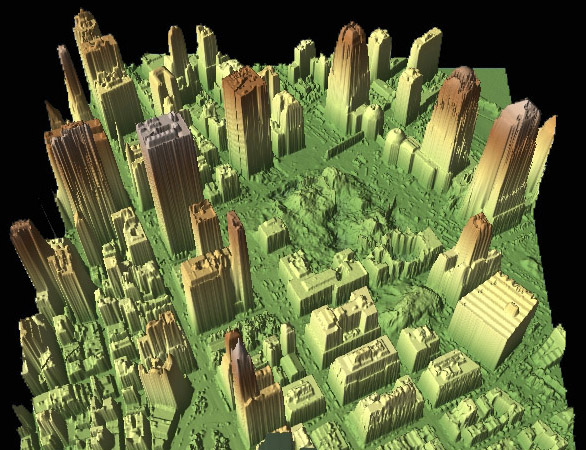
\includegraphics[width=.5\textwidth]{Fuentes_datos/LiDARWTC.png}
\caption{\small Modelo del World Trade Center realizado a partir de datos LiDAR tomados el d�a 27 de septiembre de 2001 (Fuente: NOAA/U.S. Army JPSD)}
\label{Fig:LiDARWTC} 
\end{figure}

En la terminolog�a del LiDAR, la imagen correspondiente al primer retorno (el de los puntos m�s altos) se conoce como Modelo Digital de Superficie (MDS), mientras que el correspondiente a la altura del suelo se conoce como Modelo Digital de Elevaciones (MDE). Veremos mucho acerca de MDE en posteriores cap�tulos de este libro. \index{Modelo Digital de Superficie}\index{Modelo Digital de Elevaciones}

En \cite{Kraus2001IASPRS} puede encontrarse una buena descripci�n del proceso de creaci�n de estas capas de elevaci�n partir de datos LiDAR.

Adem�s de la divisi�n entre activos y pasivos, otra forma de clasificar los sensores es en funci�n de la forma en la que registran la imagen. Algunos sensores poseen un �nico detector de radiaci�n que no cubre todo el ancho de la franja del terreno que se pretende recoger. Por medio de espejos oscilantes, se env�a a este detector la radiaci�n procedente de los distintos puntos a lo ancho de esa franja, de forma que se van recogiendo los distintos p�xeles de la imagen uno a uno, recorriendo esta de un lado a otro (Figura \ref{Fig:Tipos_sensores}a). Estos sensores se denominan \emph{de barrido}. 

Los denominados sensores \emph{de empuje} (Figura \ref{Fig:Tipos_sensores}b) eliminan la necesidad de utilizar espejos m�viles, ya que poseen un n�mero mayor de detectores que permiten cubrir todo el ancho de la imagen. Por ello, esta se va registrando no p�xel a p�xel, sino l�nea a l�nea.

\index{Sensores!de empuje}\index{Sensores!de barrido}

\begin{figure}[!hbt]   
\centering
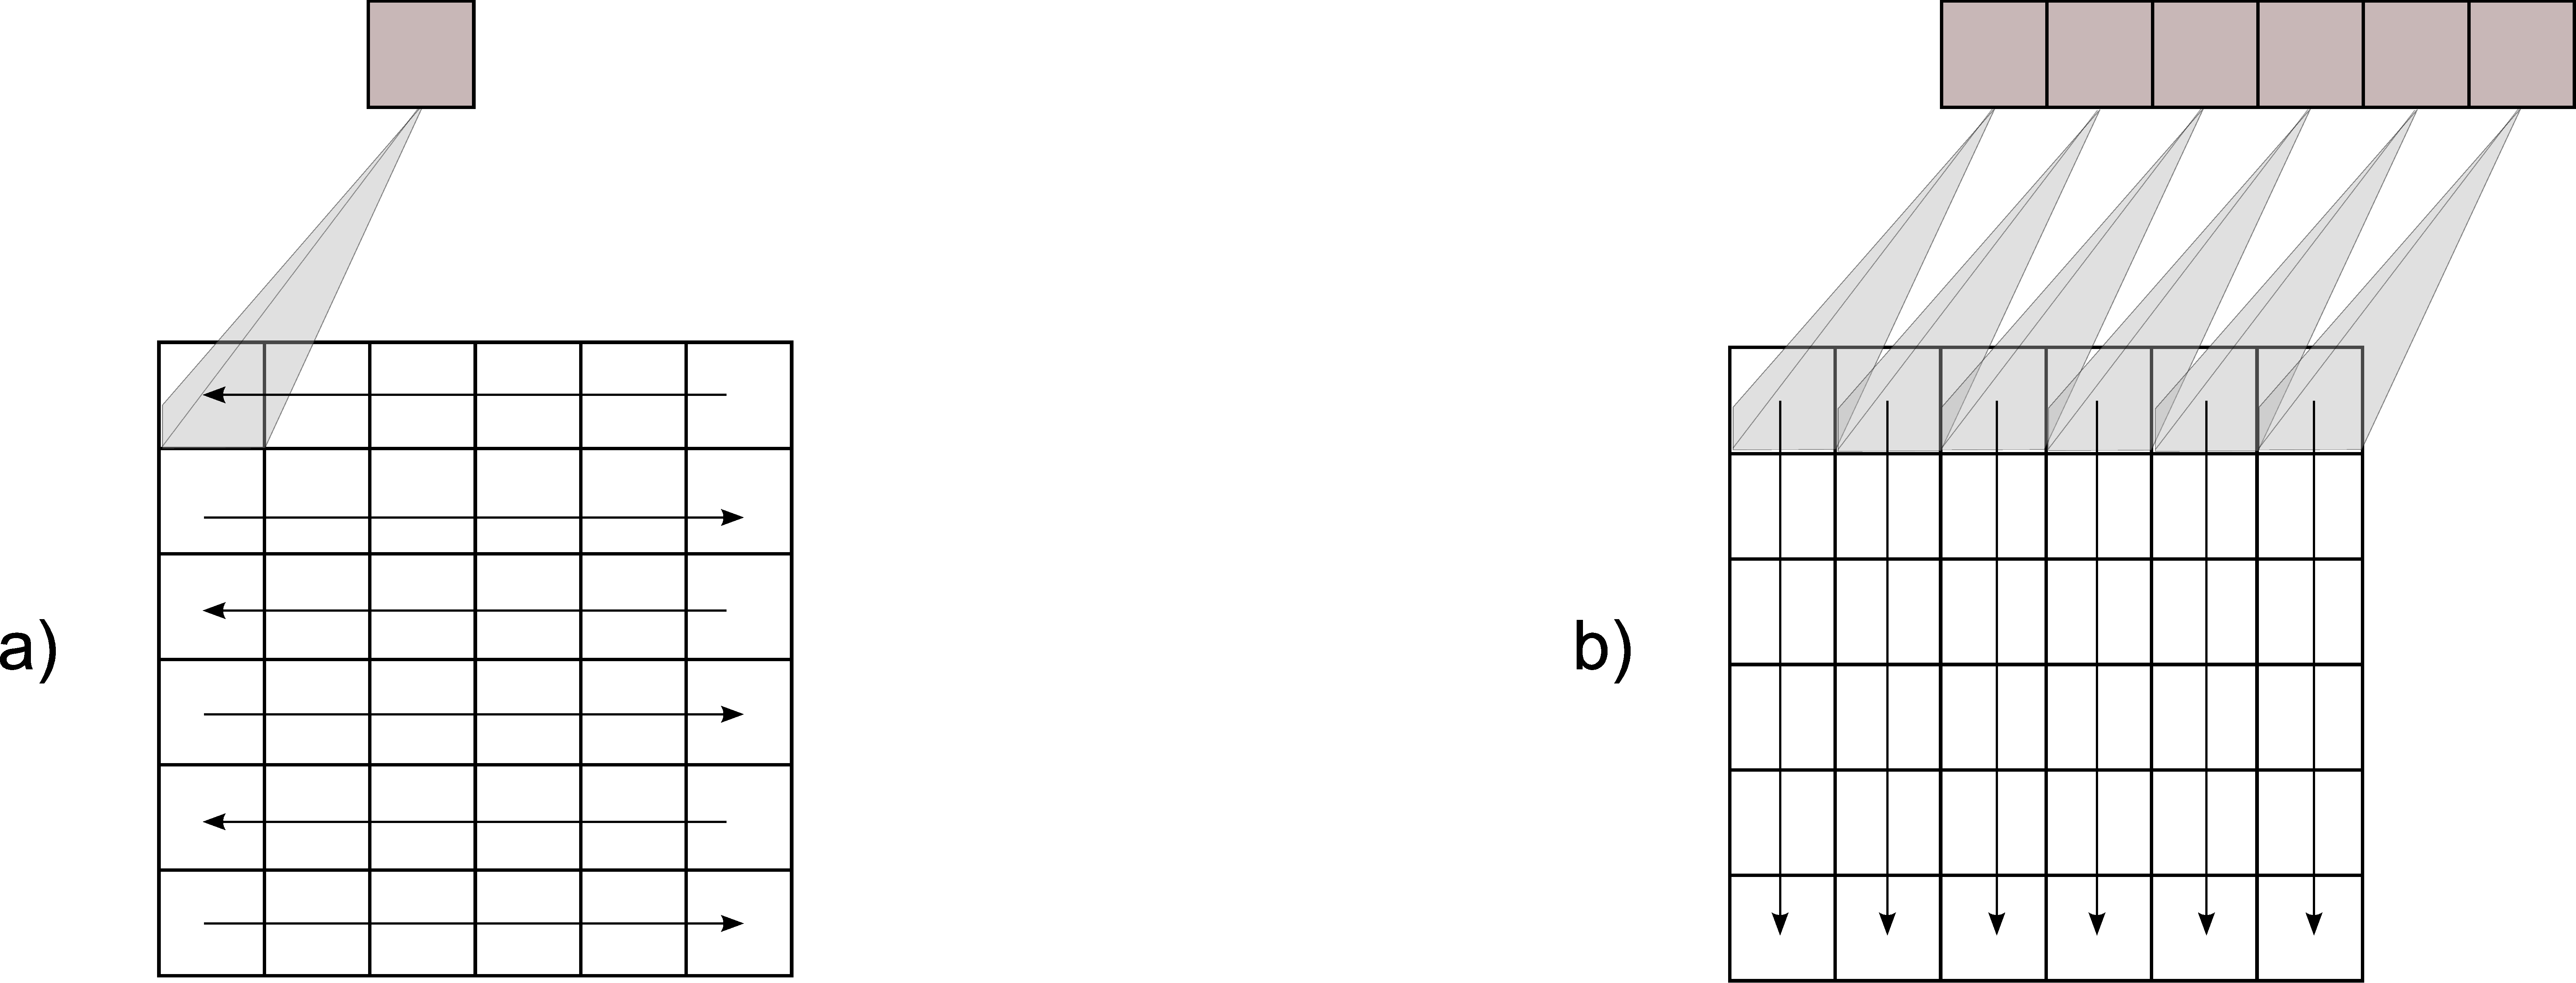
\includegraphics[width=.8\textwidth]{Fuentes_datos/Tipos_sensores.pdf}
\caption{\small Esquema de funcionamiento de un sensor de barrido (a) y uno de empuje (b)}
\label{Fig:Tipos_sensores} 
\end{figure}

\subsubsection{Resoluciones}

Uno de los par�metros principales que definen las propiedades de un sistema de teledetecci�n son las \emph{resoluciones}. Estas establecen el nivel de detalle de los productos que el sistema genera, determinando este en las distintas magnitudes en las que el sistema opera. Las resoluciones dependen del sensor y de la plataforma como binomio operativo, y de las caracter�sticas propias de ambos. Distinguimos cuatro resoluciones, a saber:

\begin{itemize}
	\item Resoluci�n espacial. Indica la dimensi�n del objeto m�s peque�o que puede distinguirse en la imagen. En l�neas generales es el equivalente al tama�o de p�xel\footnote{Desde un punto de vista formal, no ha de ser necesariamente as�, ya que la imagen puede tomarse originalmente con unas caracter�sticas y despu�s, mediante operaciones matem�ticas (veremos estas en el cap�tulo \ref{Algebra_de_mapas}), modificar el tama�o de p�xel\index{Pixel}. Aunque este tama�o sea menor al original, los objetos de menor dimensi�n que podr�n discernirse en esa imagen no ser�n iguales a ese tama�o, sino mayores.} es decir, a la dimensi�n real que un p�xel de la imagen tiene sobre el terreno.\index{Resoluci�n!espacial}
	
	La resoluci�n espacial est� en funci�n de la capacidad resolutiva del sensor y las caracter�sticas de la plataforma tales como la altura a la que se sit�a. Asimismo, la resoluci�n espacial esta relacionada con la superficie que cada imagen cubre sobre el terreno. El concepto de \emph{Campo Instant�neo de Visi�n}\footnote{Instantaneous Field of View (IFOV)} \index{Instantaneous Field of View (IFOV)} \index{Campo Instant�neo de Visi�n}indica el �ngulo de visi�n que abarca el sensor, y se utiliza habitualmente es este sentido. El \emph{Campo Instant�neo de Visi�n en Tierra}\footnote{Ground Instantaneous Field of Vision (GIFOV)}\index{Ground Instantaneous Field of Vision (GIFOV)} expresa esta misma idea pero en unidades de longitud sobre el terreno, y es funci�n del IFOV y la altura a la que se encuentre el sensor.\index{Campo Instant�neo de Visi�n en Tierra}
	
	En el dise�o de la �rbita de un sat�lite debe tenerse en cuenta el campo de visi�n del sensor para optimizar el ciclo de toma de im�genes, as� como para evitar que las distintas franjas que este cubre queden sin solaparse y existan zonas de las que no se tomen im�genes.
	
	\item Resoluci�n espectral. Todo sensor cubre una regi�n particular del espectro y almacena esta mediante un n�mero dado de bandas. La regi�n del espectro abarcada y el n�mero de bandas son los elementos que definen la resoluci�n espectral. Esta ser� elevada si el n�mero de bandas es alto, ya que cada banda cubrir� un rango de frecuencias de menor amplitud. De este modo, la informaci�n de dos frecuencias cercanas puede separarse, ya que estas ser�n recogidas en bandas distintas, mientras que si el n�mero de bandas es menor pertenecer�n a la misma banda y no podr� hacerse distinci�n alguna (la resoluci�n ser� menor).\index{Resoluci�n!espectral}
	
	En funci�n del n�mero de bandas, pueden clasificarse las im�genes y los sensores que las generan. Una imagen en blanco y negro contiene una �nica banda. Las im�genes en color contienen tres bandas, correspondientes a las frecuencias del rojo, el verde y el azul. Existen igualmente sensores con algunas bandas adicionales como la del infrarrojo, que en total generan un n�mero de bandas no superior a diez. Todas estas im�genes se conocen como \emph{multiespectrales}. 
	
	Las im�genes \emph{superespectrales} tienen una mayor resoluci�n espectral (bandas m�s estrechas), y cubren una zona del espectro m�s amplia, no limit�ndose al rango visible o el situado inmediatamente junto a este. Por ello, su n�mero de bandas es mayor, generando im�genes con varias decenas de ellas. \index{Im�genes!superespectrales}
	
	Por �ltimo, las im�genes \emph{hiperespectrales} presentan m�s de cien bandas, lo cual permite una caracterizaci�n espectral sumamente precisa.\index{Im�genes!superespectrales}
	\item Resoluci�n radiom�trica. Para cada una de las bandas que produce un sensor (asociada esta a una determinada regi�n del espectro seg�n su resoluci�n espectral), el dato recogido, que constituye su Nivel Digital, indica la intensidad correspondiente a esa regi�n. El nivel de detalle con el que puede medirse esa intensidad es el que define la resoluci�n radiom�trica del sensor.\index{Resoluci�n!radiom�trica}
	
	El n�mero de Niveles Digitales\index{Niveles Digitales} distintos que pueden recogerse es la medida de la resoluci�n espacial, y habitualmente es una potencia de dos (de la forma $2^n$). Tanto las im�genes en blanco y negro como las im�genes en color trabajan con 256 ($2^8$) niveles, ya que este es el valor m�s cercano al n�mero de diferentes intensidades que el ojo humano puede diferenciar\footnote{En el �mbito del tratamiento de im�genes esto se conoce como \emph{profundidad de color}. Una mayor profundidad de color indica mayor n�mero de colores posibles. Una pantalla normal de ordenador puede mostrar un total de 16.7 millones de colores distintos , que corresponden a las combinaciones entre los 256 posibles niveles de cada una de las tres bandas ($256 ^3 = 16,777,216$)}. No obstante, los sensores de teledetecci�n pueden tener una mayor resoluci�n radiom�trica (hasta 1024 o 2048 niveles), que si bien no se aprecia en la representaci�n visual, s� que supone una diferencia en el tratamiento anal�tico de esos Niveles Digitales.
	En la figura \ref{Fig:Resolucion_radiometrica} puede apreciarse la diferencia entre dos im�genes, cada una de las cuales tiene una resoluci�n radiom�trica distinta.

\begin{figure}[!hbt]   
\centering
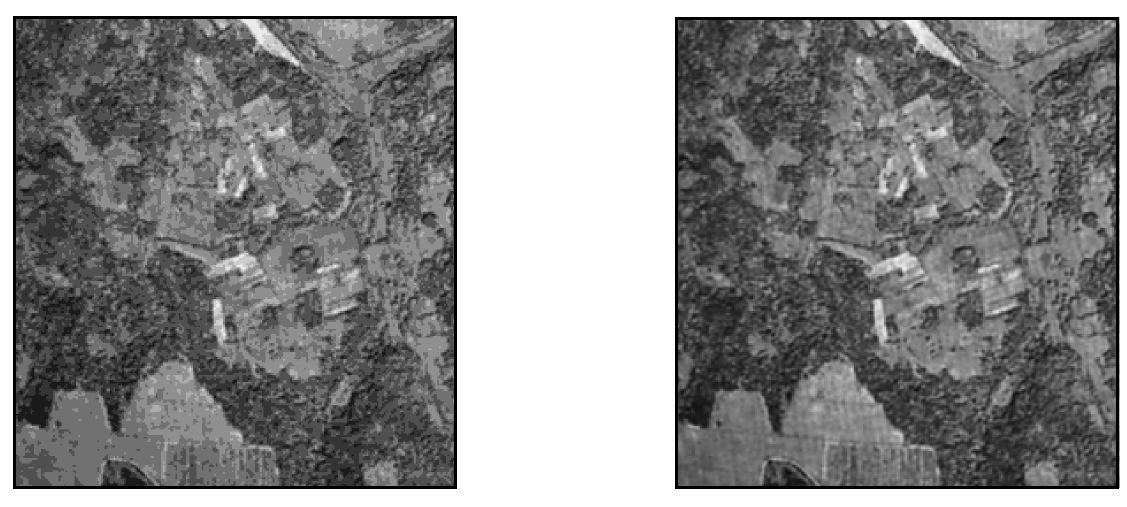
\includegraphics[width=.8\textwidth]{Fuentes_datos/Resolucion_radiometrica.png}
\caption{\small Dos imagenes con distinta resoluci�n radiom�trica (de izquierda a derecha, 8 y 256 niveles, respectivamente).}
\label{Fig:Resolucion_radiometrica} 
\end{figure}

	\item Resoluci�n temporal. Indica el tiempo que tarda el sensor en volver a tomar una imagen de una misma zona.  Tiene sentido en el caso de sensores orbitales, que funcionan por ciclos, y tras concluir este ciclo,  vuelven a comenzar la toma de im�genes en el mismo punto. En cada ciclo, el sensor cubre toda la superficie terrestre <<barriendo>> esta en franjas sucesivas.
	
	La resoluci�n temporal depende de la altura a la que se encuentra la plataforma que monta el sensor, as� como la resoluci�n espacial. Si el tama�o de las im�genes es reducido (GIFOV peque�o), las franjas son m�s estrechas y se requieren m�s para cubrir toda la superficie y volver a comenzar el ciclo, con lo que la resoluci�n espacial ser� menor.
\end{itemize}

Parece l�gico pensar que lo ideal en toda circunstancia ser�a disponer de im�genes procedentes de sistemas con altas resoluciones en cualquiera de las clases anteriores. De esta forma, tendr�amos im�genes con gran detalle espacial, espectral y radiom�trico, y actualizadas frecuentemente. No obstante, la tecnolog�a actual no dispone de elementos que ofrezcan resoluciones elevadas en todas las magnitudes del proceso, y en la creaci�n de los sensores se favorecen unas en detrimento de otras. Algunas resoluci�n presentan adem�s un cierto antagonismo, como hemos visto para las resoluciones espacial y temporal, con lo que no resulta viable que ambas sean elevadas simult�neamente.

As�, existen sensores con, por ejemplo, gran resoluci�n espacial, en los cuales la resoluci�n espectral no es tan elevada. Por el contrario, los sensores con mayor resoluci�n espectral no suelen ofrecer un nivel de detalle espacial tan elevado como los anteriores. En ocasiones, una misma plataforma puede montar a bordo varios sensores, de tal forma que el conjunto de ellos ofrezca informaci�n detallada de forma global, pero un �nico sensor no proporciona resoluci�n elevada en todas las variables.

Otro tipo de circunstancias relativas al sensor afectan igualmente a las resoluciones. Por ejemplo, aquellos sensores que trabajan con radiaciones de poca energ�a (en la regi�n de las microondas) y son de tipo pasivo requieren una amplia extensi�n para recoger la suficiente energ�a como para poder ser detectada por dicho sensor. Por esta raz�n, su resoluci�n espacial suele ser baja. 

A la hora de utilizar im�genes de teledetecci�n, debe considerarse qu� tipo de resoluci�n  resulta de mayor inter�s para el proyecto que se lleva a cabo, teniendo en cuenta la escala de trabajo o el objetivo final que se persigue con el an�lisis a realizar, entre otros factores. En base a esto, se escoger� uno u otro producto, que ser� el que ofrezca los valores de resoluci�n m�s adecuados en conjunto.

Si se pretende localizar elementos de peque�o tama�o, es imprescindible trabajar con altas resoluciones espaciales. Si lo que se desea es clasificar una serie de zonas en funci�n de sus caracter�sticas, la resoluci�n espectral debe ser alta, ya que, como veremos, se usa la informaci�n de todas las bandas para dar esa clasificaci�n, y un n�mero mayor de bandas dar� como resultado una mayor precisi�n.\index{Bandas}

De igual, modo, la detecci�n de cambios de intensidad en una banda hace necesario que se trabaje con una buena resoluci�n radiom�trica, pero si lo que se desea es estudiar esos cambios a lo largo de un periodo corto de tiempo, trabajar con un sensor con gran resoluci�n temporal se hace imprescindible.

En cada caso, las circunstancias particulares del trabajo condicionan la elecci�n de uno u otro sensor, puesto que, como se ha dicho, un �nico sensor no ofrece elevadas resoluciones en todas las variables.

La utilizaci�n simult�nea de datos de varios sensores en un proyecto es una alternativa en ciertos casos. Como veremos, existen t�cnicas que permiten combinar im�genes con alta resoluci�n espacial e im�genes con alta resoluci�n espectral, con objeto de obtener nuevas im�genes que combinen lo mejor de ambas y ofrezcan un nivel de detalle conjunto mayor. Estas t�cnicas realizan el proceso conocido como \emph{fusi�n de im�genes}, el cual trataremos en el apartado  \ref{Fusion_imagenes}, m�s adelante en este libro. \index{Im�genes!fusi�n de}\index{Fusi�n de im�genes}

Adem�s de lo anterior, un �nico sensor montado a bordo de un sat�lite puede operar en varios \emph{modos} distintos. Es habitual que un sensor multibanda pueda registrar tambi�n im�genes de una sola banda, recogiendo en ella la intensidad de la radiaci�n correspondiente a todo el espectro visible, de tal forma que genere una representaci�n visual real. Estas se suelen representar habitualmente en escala de grises, resultando una imagen en blanco y negro.

Las im�genes de este tipo se conocen como \emph{pancrom�ticas}\footnote{El t�rmino \emph{pancrom�tico} deriva de la fotograf�a cl�sica, conoci�ndose as� al tipo de pel�cula sensible a todas las longitudes de onda del visible. Por similitud de conceptos, se emplea el t�rmino tambi�n para hacer referencia a las im�genes digitales monobanda generadas por sensores seg�n lo comentado anteriormente}, y suelen tener mayor resoluci�n espacial, por lo que pueden emplearse para la fusi�n de im�genes se�alada anteriormente. As�, un mismo sensor provee todos los datos necesarios para llevar a cabo ese proceso, tanto la imagen de gran resoluci�n espacial (la pancrom�tica) como la de gran resoluci�n espectral (la imagen multibanda).
\index{Im�genes!pancrom�ticas}

\subsection{Principales sensores y productos}

El n�mero de diferentes productos provenientes de la teledetecci�n es muy elevado en la actualidad. Ahora que ya conocemos los fundamentos del proceso y las principales caracter�sticas de un sistema de teledetecci�n, es interesante mostrar un peque�o resumen de los principales productos disponibles. En ocasiones, desconocer la existencia de productos adecuados puede suponer la realizaci�n incorrecta o de modo ineficaz de un proyecto SIG, y dada la gran variedad existente, esto sucede con frecuencia. 

A continuaci�n se relacionan algunos de los sistemas de teledetecci�n principales y las caracter�sticas de sus productos.

\begin{itemize}
	\item LANDSAT \cite{webLandsat}. Se trata de un programa completo de adquisici�n de datos mediante teledetecci�n, que ha lanzado hasta la fecha un total de siete sat�lites entre 1972 y 1999. Por ello, el volumen de datos recogido es enorme, y lo convierte en una de las fuentes de datos m�s ricas  de entre las existentes en la actualidad. \index{Landsat}

	El �ltimo sat�lite, LANDSAT 7, tiene una �rbita helios�ncrona y una resoluci�n temporal de 16 d�as. A bordo de �l se monta el sensor ETM+\footnote{Enhanced Thematic Mapper Plus}, que permite la obtenci�n de im�genes pancrom�ticas con resoluci�n de 15 metros, e imagenes multibanda con resoluci�n de 60 metros. El sensor recoge un total de 8 bandas, y el tama�o de la imagen es de 170 $\times$ 183 km.

	Los sensores TM\footnote{Thematic Mapper} y MSS \footnote{Multispectral Scanner} se montan a bordo del sat�lite LANDSAT 5, todav�a en funcionamiento y con una resoluci�n temporal de 16 d�as. El sensor TM ofrece im�genes multibanda de 7 bandas con resoluci�n de 30 metros, excepto en la banda del infrarrojo t�rmico, donde la resoluci�n es de 120 metros. Las im�genes tienen un tama�o de 185 $\times$ 172 km.\index{TM (sensor)}\index{MSS(sensor)}
	\item IKONOS \cite{webIkonos}. Este sat�lite, lanzado en 1999, monta un sensor con resoluci�n de 1 metro para im�genes pancrom�ticas y 4 metros para im�genes multibanda (4 bandas). Las im�genes cubren una �rea de 11 $\times$ 11 km y el sat�lite tiene una resoluci�n temporal de entre 3 y 5 d�as.\index{IKONOS}
	\item SPOT\footnote{Satellite Pour l' Observation de la Terre} \cite{webSPOT}. Un conjunto de sat�lites lanzados inicialmente por la agencia espacial francesa, con especial �nfasis en la recogida de informaci�n relativa a variables ambientales. De los cinco puestos en �rbita, dos siguen actualmente en funcionamiento. El �ltimo de ellos, lanzado en 2002, monta el sensor HRG con capacidad de producir im�genes pancrom�ticas con resoluci�n entre 2,5 y 5 metros, e im�genes multibanda con resoluci�n de 10 metros. El periodo de revisita es de entre 1 y 4 d�as.
	Es de destacar que el sensor permite inclinaciones de hasta 27\degree respecto al nadir hacia ambos lados, por lo que puede cubrir una banda m�s ancha y tomar im�genes fuera del �rea determinada en cada instante por la �rbita.\index{SPOT}\index{Satellite Pour l' Observation de la Terre}
	\item QuickBird. \cite{webQuickbird}. Ofrece im�genes en pancrom�tico y multibanda (azul, verde, rojo e infrarrojo cercano). Las primeras tiene una resoluci�n de 60 cm y las multibanda de 2,4 metros, aunque combinando las dos ofrece im�genes en color con 60 cm de resoluci�n. 
	La �rbita del sat�lite es helios�ncrona y la resoluci�n temporal var�a entre los 3 y 7 d�as. Cada imagen cubre una superficie de 16,5 $\times$ 16,5 km.\index{QuickBird}
	\item Aqua y Terra. Dos sat�lites lanzados por la NASA dentro de un proyecto de �mbito internacional para la observaci�n de la Tierra. Cada uno de ellos monta una serie de diversos sensores, que recogen informaci�n relativa al ciclo hidrol�gico (en el caso del Aqua) y la superficie terrestre (en el caso del Terra). Entre estos sensores cabe destacar el MODIS, a bordo de ambos, o el ASTER, a bordo del sat�lite Terra. ASTER \footnote{Advanced Spaceborne Thermal Emission and Reflection Radiometer} recoge informaci�n en 14 bandas distintas, con una resoluci�n entre 15 y 90 metros, mientras que MODIS\footnote{Moderate Resolution Imaging Spectroradiometer} es un sat�lite de menor resoluci�n espacial (250, 500 o 1000 metros seg�n la banda ), 36 bandas y una resolucion temporal de 1 a 2 d�as. \index{Aqua}\index{Terra}\index{NASA}\index{ASTER}\index{MODIS}

	Adem�s de los datos directos de los sensores, se proporcionan de forma gratuita numerosos productos derivados, lo que lo convierte en una fuente de datos de primer orden para un gran n�mero de aplicaciones, especialmente las relacionadas con el estudio del medio, la vegetaci�n, etc. En la direcci�n Web \cite{webModisData} pueden obtenerse tanto datos originales como productos derivados.
	\item NOAA--AVHRR\footnote{Advanced Very High Resolution Radiometer}. Se encuentra principalmente enfocado al estudio de los oc�anos, aunque sus datos pueden aplicarse en muchos m�s estudios. El sensor tiene una resoluci�n de 1,1 km, y proporciona im�genes de 5 bandas en las regiones del infrarrojo y el visible. La resoluci�n temporal es de medio d�a, produciendo una imagen nocturna y otra diurna.\index{NOAA-AVHRR}
	\item RADARSAT. Desarrollado por la Agencia Espacial Canadiense, monta un radar de apertura sint�tica (SAR), y su principal prop�sito es el control de las variaciones ambientales y de los recursos naturales. M�s informaci�n en \cite{webRADARSAT}.\index{RADATSAT}\index{Radar de Apertura Sint�tica}\index{SAR}
	\item ERS--1 y ERS--2. Desarrollados por la Agencia Espacial Europea. Al igual que el anterior, ambos est�n pensados para la observaci�n medioambiental, y montan tanto sensores activos como pasivos. M�s informaci�n en \cite{webERS2}.\index{ERS--1}\index{ERS--2}
	\item SRTM. La misi�n SRTM\footnote{Shuttle Radar Topography Mission} es un proyecto internacional de gran envergadura destinado a la creaci�n de una cobertura de elevaciones a nivel mundial. Utilizando sensores basados en radar montados sobre una lanzadera espacial, se realiz� un vuelo global de la superficie terrestre a lo largo de 11 d�as, recogiendo el relieve de todas las zonas situadas entre los 56 grados sur y los 60 grados norte de latitud. La resoluci�n de los datos obtenidos es de un segundo de arco (aproximadamente 30 metros), aunque solo se encuentran disponibles para Estados Unidos, siendo de unos 90 metros en el resto de zonas. Los datos SRTM se pueden descargar gratuitamente en \cite{webSRTMDownload}. M�s informaci�n sobre el proyecto puede encontrarse en \cite{webSRTM}. \index{SRTM}\index{Shuttle Radar Topographic Mission}
\end{itemize}

\section{Cartograf�a impresa. Digitalizaci�n}

\index{Digitalizaci�n}

La primera fuente de cartograf�a de la que se dispon�a en las etapas iniciales de los SIG era la  cartograf�a impresa. No se trataba de elementos creados pensando en su utilizaci�n dentro de un SIG y, de hecho, su estructura no es, como veremos, la m�s adecuada para ser incorporados como datos de trabajo en un SIG. Se trata, por tanto, de una clara fuente secundaria de datos espaciales. Aun as�, esta fuente era la fuente principal de informaci�n cartogr�fica disponible entonces, y su uso ha sido desde esos tiempos una constante dentro del �mbito SIG.

A pesar de que hoy en d�a disponemos de otras fuentes cartogr�ficas, la cartograf�a impresa sigue siendo b�sica para trabajar con un SIG, ya que existe mucha informaci�n que todav�a solo se encuentra en este formato. De una u otra forma, es probable que un proyecto SIG implique en alg�n punto de su desarrollo la necesidad de recurrir a cartograf�a impresa y tratar esta para su inclusi�n dentro de un SIG.

Cuando hablamos de cartograf�a impresa, no hay que pensar �nicamente en mapas o planos, sino tambi�n en im�genes tales como fotograf�as a�reas, las cuales, dependiendo de su antig�edad, pueden encontrarse disponibles tan solo en formato impreso, como hemos visto. Mientras que resulta posible adquirir estas en formato digital cuando se trata de fotograf�as m�s actuales, la tomadas por m�todos anal�gicos correspondientes a vuelos m�s antiguos solo pueden adquirirse por regla general como un producto impreso.

Los procesos que permiten obtener un producto digital a partir de esas im�genes son costosos en tiempo y dinero, y es por ello que no todos los proveedores de estas ofrecen la posibilidad de adquisici�n de un producto digital. En esta secci�n veremos esos procesos, tanto si partimos de un mapa o plano como si partimos de una imagen o cualquier otro documento impreso que pueda contener informaci�n cartogr�fica, susceptible de ser convertida en una o varias capas seg�n se requieren para el trabajo en un SIG.

Ya conocemos los dos modelos de datos con los que trabajamos en un SIG: el modelo r�ster y el modelo vectorial. Tanto mapas como fotograf�as a�reas pueden servir como fuente de informaci�n para crear o bien capas r�ster o bien capas vectoriales, ya que la informaci�n que contienen puede de igual modo representarse seg�n uno u otro modelo (debe recordarse que, como se mencion� en el cap�tulo \ref{Tipos_datos}, puede convertirse una capa r�ster en vectorial y viceversa mediante algoritmos que detallaremos m�s adelante en este libro).\index{Conversi�n!r�ster--vectorial}

Un mapa o plano sobre un soporte impreso, sin embargo, dista considerablemente de ese concepto de capa con el que trabajamos en un SIG. Suele contener informaci�n sobre distintas variables, tales como carreteras, elevaci�n, n�cleos urbanos, uso de suelo, y todas ellas en un �nico elemento cartogr�fico. Esas variables, que en un SIG manejar�amos como capas independientes, se presentan como un conjunto que, seg�n el uso que queramos darle, va a ser mucho m�s conveniente disgregar en base a esas distintas variables.

Si pensamos en una fotograf�a a�rea, esta puede considerarse como una simple imagen dentro de un SIG, y como vimos en el cap�tulo \ref{Tipos_datos}, las im�genes se adaptan al modelo de representaci�n r�ster. Por otra parte, en esa imagen existir�n elementos tales como carreteras, r�os o �rboles, los cuales se representan mejor seg�n el modelo vectorial. En funci�n de qu� informaci�n nos interese tener dentro de un SIG o el modelo de representaci�n preferente que queramos manejar, las operaciones que debemos llevar a cabo ser�n unas u otras.

Este conjunto de operaciones posibles se conocen como de \emph{digitalizaci�n}, y en funci�n de la forma en que se desarrollen podemos distinguir los siguientes tipos:

\begin{itemize}
	\item Digitalizaci�n autom�tica 
	\item Digitalizaci�n manual
\end{itemize}

\index{Digitalizaci�n!tipos}

En la digitalizaci�n autom�tica, el sistema (inform�tico o mec�nico) se encarga de generar los elementos digitales que ya podremos incorporar a un SIG, ahorrando trabajo al operador al automatizar la tarea. Este tipo de digitalizaci�n es muy habitual para el caso de obtener un resultado r�ster mediante el proceso de \emph{escaneo}\index{Escaneo}. Tambi�n resulta posible automatizar la digitalizaci�n para el caso vectorial, aunque requiere cierta labor por parte del operario y no es un proceso tan sencillo, pudiendo obtenerse resultados desiguales. 

La digitalizaci�n manual requiere por parte del operario una definici�n expl�cita de los elementos a crear, y es por ello �nicamente adecuada para obtener un resultado vectorial, traz�ndose las entidades (sean estas puntos, l�neas o pol�gonos) manualmente mediante alg�n sistema que permita esa introducci�n de datos. 

La elecci�n de uno u otro tipo de digitalizaci�n no depende solo del tipo de capa que se desee obtener. Tanto la digitalizaci�n manual como la autom�tica, tienen cada una de ellas su propias ventajas. En el caso r�ster la opci�n manual no es viable, pero al digitalizar un mapa para obtener una capa vectorial puede ser interesante optar por una o otra metodolog�a en funci�n de las circunstancias. 

La digitalizaci�n manual es mucho m�s costosa y su resultado es muy variable en cuanto a su precisi�n espacial, ya que depende en gran medida de la experiencia del operario y de las condiciones de este (cansancio, circunstancias personales, etc.). Por el contrario, e independientemente del operario, el reconocimiento de las entidades es altamente fiable (si se trata de un mapa, este ha sido dise�ado para ser interpretado por una persona, por lo que esta reconocer� sus elementos sin dificultad y con total fiabilidad). 

Asimismo, un proceso autom�tico, en caso de proceder de forma correcta, tendr� una exactitud absoluta y <<clonar�>> con absoluta fidelidad los elementos del mapa impreso. Esto resulta una ventaja a la hora de obtener una gran precisi�n, pero impide que en el proceso de digitalizaci�n se puedan corregir errores existentes en el documento original. Un operario puede advertir esos errores y corregirlos a medida que digitaliza. Un sistema autom�tico, por el contrario, no puede.
 
\subsection{Digitalizaci�n manual}\label{Digitalizacion_manual}\index{Digitalizaci�n!manual}

La digitalizaci�n manual es la forma m�s b�sica de crear informaci�n digital a partir de un documento cartogr�fico impreso. Un operario trabaja directamente sobre la fuente cartogr�fica y su trabajo se traduce en la creaci�n de una nueva capa, gracias a la utilizaci�n de un equipo que es capaz de convertir su trabajo en la informaci�n necesaria para crear dicha capa.

En el modelo de representaci�n r�ster, los elementos b�sicos son las celdas, que forman una malla regular que puede presentar un numero muy elevado de estas. Una definici�n manual de las caracter�sticas de cada una de esas celdas resulta inviable, por lo que la digitalizaci�n de un documento cartogr�fico impreso para la obtenci�n de una capa r�ster a partir de ella de forma manual no es factible.

Por el contrario, se puede realizar con cierta sencillez la digitalizaci�n de una entidad vectorial, trazando la forma de esta o, en caso de ser una entidad de tipo punto, sencillamente indicando su localizaci�n. Cuando el n�mero de entidades es elevado, el proceso puede llevar tiempo y ser tedioso, pero en todo caso sigue resultando una forma sencilla y accesible de crear una capa vectorial a partir de otra fuente de datos.

Para llevar a cabo ese trazado de la entidad, se necesita emplear alg�n equipo que recoja la informaci�n introducida por el operador. Existen dos alternativas principales: utilizar un equipo especializado dise�ado espec�ficamente para la digitalizaci�n, o bien digitalizar utilizando las funciones de edici�n de un GIS, realizando todo el proceso dentro de este y sin m�s herramientas que el propio ordenador y un dispositivo se�alador como el rat�n.

\subsubsection{Con equipo especializado (\emph{heads--down})} \label{heads-down}

\index{Heads--down}

La forma tradicional de proceder a la digitalizaci�n manual de entidades es utilizando equipos y perif�ricos expresamente dise�ados para llevar a cabo esta tarea. La \emph{tableta digitalizadora} (Figura \ref{Fig:Tableta_digitalizadora}) es la herramienta fundamental para este trabajo.\index{Tableta digitalizadora}

\begin{figure}[!hbt]   
\centering
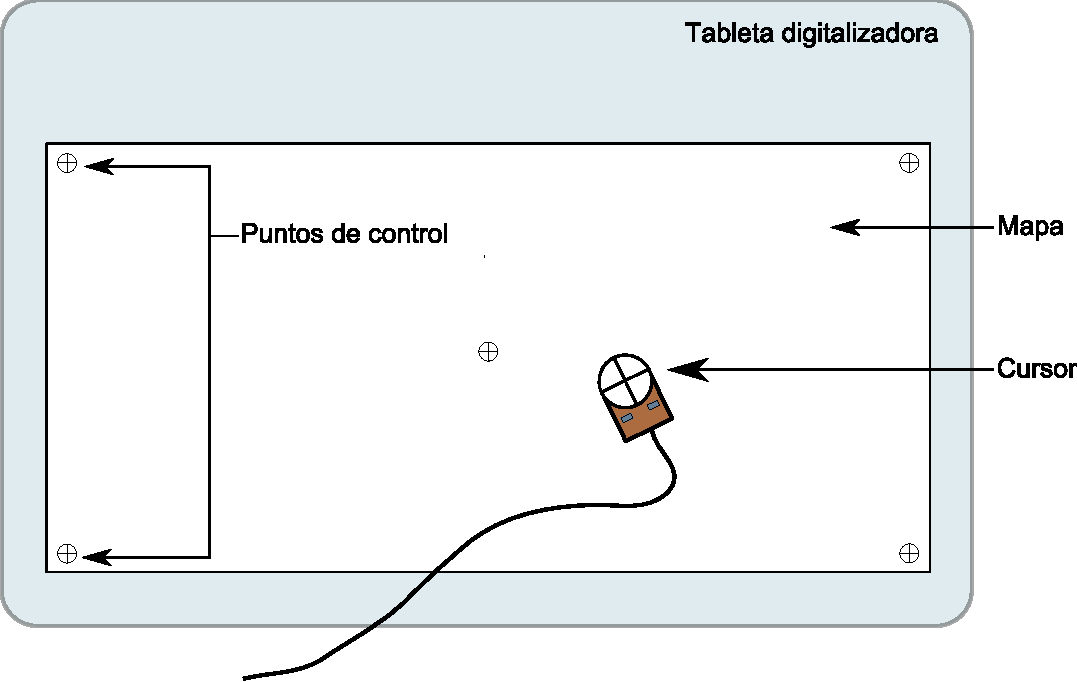
\includegraphics[width=.8\textwidth]{Fuentes_datos/Tableta_digitalizadora.pdf}
\caption{\small Esquema de una tableta digitalizadora y los elementos del proceso de digitalizaci�n.}
\label{Fig:Tableta_digitalizadora} 
\end{figure}

Se trata de una superficie plana a modo de atril, sobre la cual se sit�a el documento cartogr�fico a digitalizar, y sobre este se van trazando las distintas entidades con un cursor. Este cursor registra los movimientos del operario, convirtiendo las posiciones del cursos en coordenadas reales, que son las que van a constituir la entidad digitalizada. El trabajo del operario consiste en seguir con el cursor las formas de las distintas entidades, como si las estuviera calcando, de modo que indique al sistema las geometr�as que se quieren definir.

El proceso de digitalizaci�n implica los siguientes pasos \cite{Heywood1998Longman}:

\begin{itemize}
	\item Registro. La etapa fundamental del proceso, que garantiza que las coordenadas de las entidades digitalizadas sean correctas. El mapa se ha de adherir a la tableta de modo firme, normalmente con cinta adhesiva u otro medio similar, y se�alar en �l unos \emph{puntos de control} de coordenadas conocidas. Ser� en base a estos como se calcularan las restantes coordenadas de las entidades que el operario defina mediante el cursor. Habitualmente se utilizan como puntos de control las esquinas y alg�n punto central del mapa. Es importante que en el proceso de registro el mapa no presente dobleces o deterioros que puedan inducir errores en el c�lculo de coordenadas posteriores.\index{Puntos!de control}
	\item Digitalizaci�n de entidades puntuales.
	\item Digitalizaci�n de entidades lineales.
	\item Digitalizaci�n de entidades poligonales.
	\item Asignaci�n de atributos. A cada una de las entidades digitalizadas se le a�aden sus correspondientes propiedades. Este paso no se realiza ya con la tableta digitalizadora.
	En el caso m�s general, estos atributos se introducen manualmente con el teclado o se toman, por ejemplo, de una base de datos. Un caso particular, no obstante, es el de la digitalizaci�n de curvas de nivel. Una vez que estas han sido digitalizadas, no es necesario asignar valores individualmente a cada una de las lineas, ya que entre ellas existe una relaci�n que puede aprovecharse para simplificar el establecimiento de una cota correspondiente a cada una. Estableciendo la elevaci�n de una y la direcci�n en que la elevaci�n aumenta, pueden sistem�ticamente asignarse elevaciones a las curvas que aparecen seg�n se avanza en dicha direcci�n. Los SIG m�s populares presentan habitualmente herramientas que facilitan este proceso.
\end{itemize}

Esta forma de digitalizar se conoce como <<cabeza abajo>> (\emph{heads--down}), en referencia a la posici�n del operario a la hora de trabajar sobre la tableta.

Se distinguen dos formas principales de registro de puntos:

\begin{itemize}
	\item Manual. El usuario debe ir marcando uno por uno todos los puntos que desee incorporar a la entidad digitalizada. Por ejemplo, para el caso de una l�nea, debe ir deteniendo el rat�n regularmente en aquellos puntos que considere de inter�s, y sobre ellos pulsando los botones del cursor para indicar al sistema que ha de registrar dichos puntos.
	\item Semiautom�tica. El operario simplemente desliza el cursor definiendo la forma de los entidades, y el propio sistema se encarga de almacenar puntos regularmente seg�n un intervalo de tiempo definido. Esto permite un ahorro de tiempo considerable y una correcta densidad de puntos recogidos para cada entidad.	
\end{itemize}

Las tabletas digitalizadoras son elementos caros, motivo por el cual se tiende a favorecer en la actualidad la digitalizaci�n en pantalla, que presenta adem�s otra serie de ventajas adicionales, como seguidamente veremos.
 
\subsubsection{En pantalla (\emph{heads--up})}

\index{Heads--up}

La otra forma de digitalizar elementos es utilizando las capacidades de edici�n de un SIG. Estas capacidades son heredadas de las aplicaciones de dise�o asistido por ordenador (CAD)\index{CAD}, y permiten <<dibujar>> en la pantalla del ordenador entidades y formas tales como los puntos, l�neas y rectas que constituyen los objetos en el modelo de representaci�n vectorial.

En este proceso se parte igualmente de un capa base, generalmente una imagen, y bas�ndose en ella se van definiendo los objetos, <<dibuj�ndolos>> sobre la pantalla, una vez m�s como si se calcara aquello que puede visualizarse en dicha imagen. El hecho de que un SIG nos permita tener varias capas simult�neamente y visualizarlas a voluntad, facilita el proceso de digitalizaci�n. Tambi�n lo facilita el poder tener varias im�genes sobre el fondo (cada una de ellas como una capa individual), de modo que podemos cubrir un �rea m�s amplia que la de una simple hoja de mapa o una �nica imagen.

En este proceso, no partimos en realidad de un documento cartogr�fico anal�gico, pues ya ha sido necesario digitalizarlo de alguna forma para incorporarlo en un SIG. El proceso es una digitalizaci�n de las entidades como tales, pero la informaci�n ya ha de estar en formato digital, aunque no en el modelo de representaci�n vectorial, sino en el modelo r�ster. Por ello, puede utilizarse como capa de partida una imagen originalmente en formato digital o bien una imagen originalmente en formato impreso. En este ultimo caso, la imagen ha debido digitalizarse previamente mediante un proceso de \emph{escaneo}, el cual se tratar� en la siguiente secci�n.

En la figura \ref{Fig:Digitalizacion_en_pantalla} puede verse un ejemplo de la digitalizaci�n de una imagen en pantalla.

\begin{figure}[!hbt]   
\centering
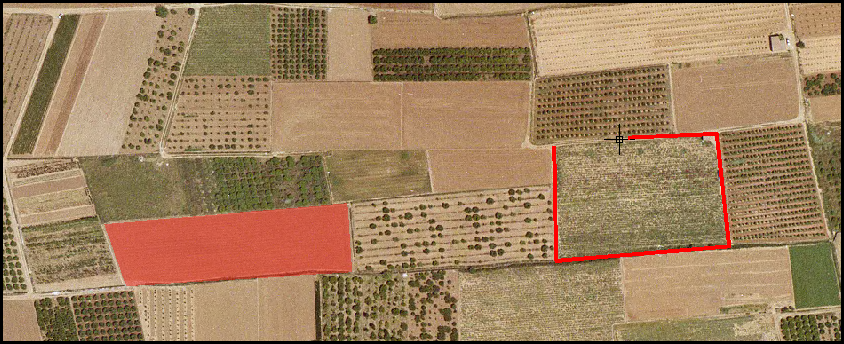
\includegraphics[width=.8\textwidth]{Fuentes_datos/Digitalizacion_en_pantalla.png}
\caption{\small Digitalizaci�n en pantalla. En rojo, pol�gono ya digitalizado. Las lineas rojas indican un nuevo pol�gono, actualmente en edici�n}
\label{Fig:Digitalizacion_en_pantalla} 
\end{figure}

En la figura, sobre una imagen a�rea en color se digitalizan las distintas parcelas que pueden distinguirse en esta. Del mismo modo, pueden digitalizarse curvas de nivel en un mapa escaneado, u otras entidades tales como r�os, lagos o v�as de comunicaci�n sobre una fotograf�a a�rea, entre muchas otras. La digitalizaci�n en pantalla puede incluso utilizarse teniendo como base no una imagen, sino capas de cartograf�a vectorial o cualquier capa de datos que aporte alg�n tipo de informaci�n que pueda delinearse con las mismas herramientas de edici�n.

La digitalizaci�n en pantalla se conoce tambi�n como digitalizaci�n <<cabeza arriba>> (\emph{heads--up}), ya que el operador centra su atenci�n en la pantalla, con una postura bien distinta a la que se tiene al trabajar con una tableta digitalizadora.

Frente a dicho trabajo con tableta digitalizadora, la digitalizaci�n en pantalla tiene las siguientes ventajas:

\begin{itemize}
	\item Menor coste. No se requiere equipo especializado de alto coste, ya que basta con un ordenador personal. 
	\item Posibilidad de dividir el trabajo. Cuando se trabaja con un mapa sobre una tableta digitalizadora, este mapa no puede ser utilizado por otro operario. Sin embargo, el uso de una capa digital dentro de un SIG como base para la digitalizaci�n, permite que varios operarios trabajen con ella simult�neamente y se repartan el trabajo.
	\item Posibilidad de correcci�n y edici�n precisa. Las mismas capacidades que se usan para trazar las distintas entidades puede emplearse para corregir o modificar estas una vez que estas ya han sido digitalizadas (Figura \ref{Fig:Correccion_digitalizacion}), resultando esto en un proceso de digitalizaci�n m�s flexible.
	\item Posibilidad de ampliaci�n. Para cartograf�as de baja calidad, puede ser dif�cil obtener precisi�n si se trabaja directamente sobre el mapa, as� como si los elementos a digitalizar son peque�os, requiri�ndose del operador un esfuerzo visual adicional. Las capacidades que tiene todo SIG para ampliar una imagen (\emph{zoom}) permiten superar esta dificultad y trabajar a distintas escalas seg�n la precisi�n del trabajo a realizar o las caracter�sticas de los objetos digitalizados.
	\item Mayor precisi�n. La capacidad de resoluci�n del ojo humano es mucho menor que la resoluci�n de las im�genes (v�ase m�s adelante el apartado \ref{Condiciones_digitalizacion}). Esto, unido a lo mencionado en el punto anterior, permite aprovechar mejor la informaci�n de la fuente original, y que los resultados obtenidos en la digitalizaci�n de esta sean m�s fieles a ella.
	\item Mayor comodidad para el operario. La postura del operario es m�s adecuada cuando se digitaliza sobre la pantalla, permitiendo unas mejores condiciones. Esto que se traduce en menor cansancio y ello indirectamente comporta resultados m�s precisos.
\end{itemize}

\begin{figure}[!hbt]   
\centering
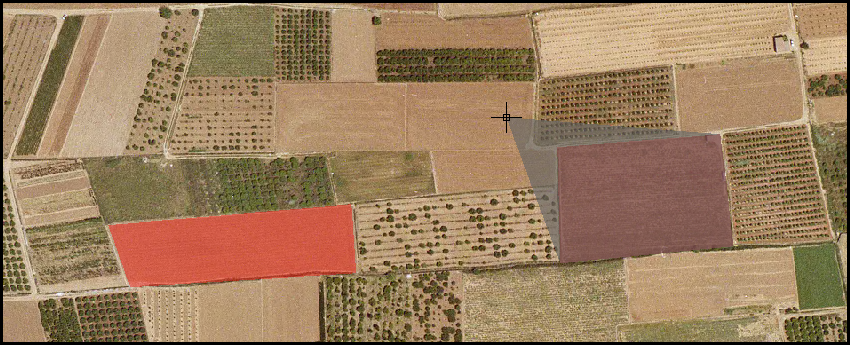
\includegraphics[width=.8\textwidth]{Fuentes_datos/Correccion_digitalizacion.png}
\caption{\small Correcci�n de entidades con las funciones de edici�n de un SIG. El pol�gono de la derecha se encuentra en edici�n, siendo modificado uno de sus v�rtices.}
\label{Fig:Correccion_digitalizacion} 
\end{figure}

Para conocer con m�s detalle las capacidades b�sicas de edici�n de un SIG, as� como las restantes capacidades que contribuyen a su vez a facilitar la labor de edici�n, cons�ltese el capitulo \ref{SIGs_escritorio}.

\subsection{Digitalizaci�n autom�tica}\index{Digitalizaci�n!autom�tica}

La digitalizaci�n autom�tica limita el trabajo del operario, ya que este no es responsable directo de definir las propiedades de los elementos que se digitalizan. Este tipo de digitalizaci�n es la  habitual en el caso de generar una capa r�ster, aunque tambi�n pueden obtenerse capas vectoriales procesando de modo autom�tico cartograf�a impresa. 

Este segundo caso, no obstante, requiere una cartograf�a en condiciones especiales, no siendo adecuada para todo tipo de mapas. En caso de no presentarse esas condiciones, los resultados de la digitalizaci�n no son �ptimos, y requieren posteriormente un gran trabajo de correcci�n y supervisi�n.

\subsubsection{Escaneo}\label{Escaneo}

\index{Escaneo}

El escaneo es el proceso de digitalizaci�n que convierte una imagen impresa (anal�gica) en una imagen digital \cite{Jackson1991Longman}. El resultado de este proceso es, por tanto, y desde el punto de vista de un SIG, una capa r�ster. Pueden escanearse tanto mapas como fotograf�as a�reas, operando en ambos casos de un modo similar y con las mismas consideraciones, pues el objeto del proceso es el mismo: la conversi�n del documento impreso en un documento digital que pueda utilizarse dentro de un SIG o cualquier otro software tal como, por ejemplo, un software de tratamiento de im�genes.

El dispositivo fundamental para realizar este proceso es el \emph{esc�ner}. Este se compone de una \emph{cabeza} sobre la que se monta un sensor, y un soporte sobre el que se desplaza o bien la cabeza o bien el documento a escanear, de tal modo que durante el proceso de escaneo esta recorre todo el documento, recogiendo la informaci�n de toda su extensi�n.\index{Esc�ner}

Este proceso de \emph{barrido} se realiza en una �nica ocasi�n, aunque dispositivos m�s antiguos pueden hacerlo en tres ocasiones a la hora de escanear documentos en color. Aunque lo habitual es la creaci�n de una imagen en color, tambi�n  pueden obtenerse im�genes en blanco y negro o en escala de grises.

Aunque existen esc�neres espec�ficamente dise�ados para el trabajo con documentos cartogr�ficos, estos son dispositivos muy especializados y de muy elevado coste. Los esc�neres m�s gen�ricos, pensados para el trabajo con todo tipo de im�genes y para todo tipo de usos, pueden no obstante emplearse de igual modo para escanear tanto mapas como im�genes a�reas con resultados aceptables, utiliz�ndose con frecuencia.

Existen tres tipos principales de esc�neres:

\begin{itemize}
	\item De sobremesa (\emph{flat--bed}). Los habituales para el uso dom�stico o el escaneo de im�genes de peque�o formato, aunque tambi�n existen de mayor tama�o. El documento a escanear se sit�a sobre una placa de cristal bajo la que se desplaza la cabeza con el sensor. Puede verse uno de estos esc�neres en la figura \ref{Fig:Escaner_sobremesa}.\index{Flat--bed}
	\item De tambor. El mapa se sit�a sobre un tambor que rota, mientras que la cabeza se mantiene fija. La figura \ref{Fig:Escaner_tambor} muestro uno de estos esc�neres.
	\item Alimentados. El sensor se mantiene fijo y el documento se desplaza mediante un mecanismo de arrastre, de forma similar a como avanza el papel en una impresora dom�stica. Salvo que dispongan de mecanismos espec�ficos para corregir esta circunstancia, suelen presentar importantes distorsiones geom�tricas causadas por un desplazamiento impreciso del papel.
\end{itemize}

\begin{figure}[!hbt]   
\centering
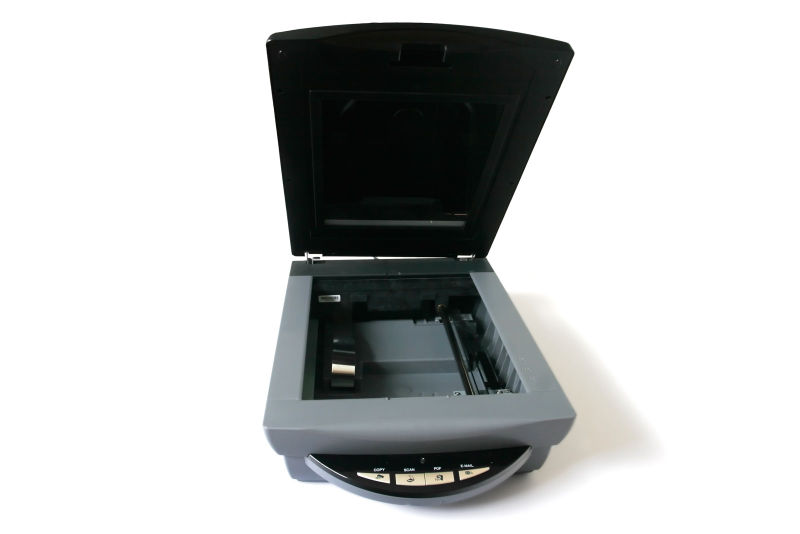
\includegraphics[width=.5\textwidth]{Fuentes_datos/Escaner_sobremesa.png}
\caption{\small Esc�ner de sobremesa (tomado de Wikipedia)}
\label{Fig:Escaner_sobremesa} 
\end{figure}

\begin{figure}[!hbt]   
\centering
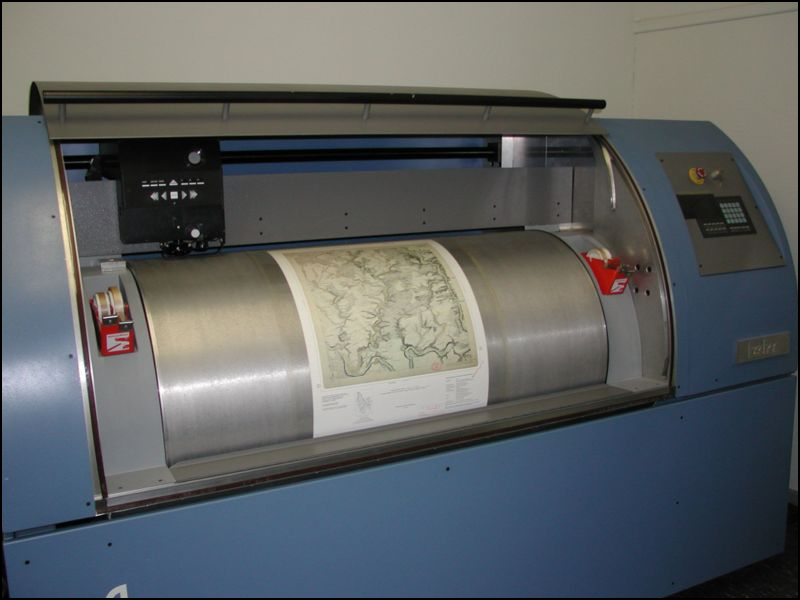
\includegraphics[width=.5\textwidth]{Fuentes_datos/Escaner_tambor.png}
\caption{\small Esc�ner de tambor (fotograf�a: Stefan Kuehn)}
\label{Fig:Escaner_tambor} 
\end{figure}

Los par�metros b�sicos que definen las caracter�sticas de un esc�ner son la resoluci�n espacial y la resoluci�n radiom�trica. La primera de estas de mide habitualmente en \emph{puntos por pulgada}\footnote{\emph{Dots per inch}(dpi)} y nos indica el n�mero de puntos (celdas) que el sensor es capaz de tomar por cada unidad de longitud sobre el papel. La resoluci�n radiom�trica, por su parte, indica la capacidad del sensor para distinguir entre dos colores distintos.\index{Dots per inch}\index{Resoluci�n!espacial}\index{Resoluci�n!radiom�trica}

A la hora de trabajar con documentos cartogr�ficos de cara a su posterior utilizaci�n en un SIG, tanto la resoluci�n espacial como la radiom�trica de los esc�neres habituales es en general m�s que suficiente, incluso en ocasiones en aquellos de uso dom�stico. No obstante, es habitual que se presenten distorsiones geom�tricas que suponen un problema importante a la hora de mantener la precisi�n cartogr�fica, y ello exige la utilizaci�n de equipos de mayor calidad si se requiere un resultado de alta precisi�n. Estos equipos no han de ser necesariamente de aquellos pensados para el trabajo con cartograf�a, sino que pueden ser de uso gen�rico, siempre, eso s�, que sean de la calidad necesaria.

La velocidad del esc�ner es otro par�metro importante, pues la preparaci�n de una base de datos cartogr�fica a partir de cartograf�a anal�gica puede llevar un tiempo considerable si el volumen de datos es elevado, ya que el proceso de escaneo es laborioso y requiere de cierto tiempo. El rendimiento del esc�ner y la velocidad a la que puede digitalizar una imagen dada est� en relaci�n directa con la resoluci�n espacial. Un esc�ner posee una resoluci�n nominal (en dpi), que es la resoluci�n m�xima a la que puede trabajar (el detalle m�ximo que puede recoger). No obstante, puede ajustarse la resoluci�n de trabajo en funci�n de las necesidades, y una resoluci�n mayor siempre lleva asociado un tiempo de proceso mayor, ya que el volumen de informaci�n generado es mayor, as� como el detalle que ha de registrarse.\index{Resoluci�n!nominal de un escaner}

Para cada documento existe una resoluci�n �ptima de escaneo en funci�n de las caracter�sticas de este. Esta resoluci�n debe elegirse teniendo en cuenta que el volumen de datos aumenta a medida que empleamos una mayor resoluci�n, buscando un equilibrio adecuado entre ese volumen de datos resultante y la cantidad de informaci�n que recogemos. Asimismo, se ha considerar igualmente el tiempo necesario para escanear el documento, tal como se dijo anteriormente.

El par�metro base es la relaci�n entre el tama�o de p�xel (la longitud real que representa el ancho de un p�xel sobre el terreno) y el tama�o de este p�xel en la imagen (lo que mide esa longitud en el mapa). Las resoluciones habituales utilizadas para el escaneo de fotograf�as a�reas var�an entre los 100 dpi ($\approx 250 \mu m$ cada punto sobre el mapa) y 2500 dpi (($\approx 10 \mu m$ cada punto sobre el mapa) \cite{Welch1996Onward}. Por ejemplo para una resoluci�n de 300 dpi, se tiene:

\begin{equation}
300 \mathrm{dpi} = \frac{300\mathrm{filas}}{2,54 \mathrm{cm\; de\; mapa}} = 118,11 \mathrm{filas/cm\; de\; mapa}
\end{equation}

En un cent�metro cuadrado se tienen $118,11^2\approx13950$ puntos.

Si trabajamos, por ejemplo, con un mapa a una escala 1:50000, tenemos que la distancia real que representa el alto de cada fila es

\begin{equation}
\frac{50000 \mathrm{cm}}{118,11 \mathrm{filas}} = 4,24 \mathrm{metros}/\mathrm{fila}
\end{equation}

Es decir, cada p�xel del mapa representa sobre el terreno un cuadrado de lado 4,24 metros.\index{Pixel}

Con c�lculos similares podemos calcular para cada posible resoluci�n el espacio real que representa, y elegir esta en funci�n del detalle que necesitemos. Como regla general, debe tratar de trabajarse con una resoluci�n que garantice que los objetos que resultan de inter�s de la imagen (por ejemplo, aquellos que van a digitalizarse despu�s manualmente mediante una digitalizaci�n en pantalla con esa imagen) sean distinguibles con claridad. 

En el caso de im�genes a�reas, la resoluci�n de estas medida en pares de lineas por mil�metro puede ser superior y permitir escanear a mayor resoluci�n, aunque ello no es estrictamente necesario, y debe una vez m�s buscarse el equilibrio entre las ventajas y los inconvenientes de trabajar con una resoluci�n m�s elevada.

En \cite{Welch1996Onward} puede encontrarse informaci�n m�s detallada sobre la elecci�n de una resoluci�n �ptima en el escaneo de im�genes a�reas.

Para el caso de mapas, no deben olvidarse los fundamentos cartogr�ficos en base a los cuales se ha creado dicho mapa, que fueron detallados en el cap�tulo \ref{Fundamentos_cartograficos}. Trabajando con una resoluci�n m�s elevada no hace necesariamente que estemos incorporando m�s informaci�n, ya que esta puede no existir en el mapa original. Tendr�amos un volumen de datos m�s elevado que el necesario para recoger toda la informaci�n del mapa.

Una diferencia fundamental entre escanear una hoja de un mapa y una imagen a�rea es la diferencia de tama�o. Los mapas suelen tener tama�os mucho mayores que los de un esc�ner com�n, lo cual obliga a utilizar equipos de gran formato o, en la mayor�a de los casos, contratar servicios de escaneo especializados, ya que estos equipos tiene un coste muy elevado. 

Una soluci�n distinta en el caso de mapas de gran tama�o es el escaneo de la hoja por partes y la posterior uni�n de las distintas partes. En este caso, es necesario asegurarse de que las partes son coherentes entre s� en lo que respecta a las condiciones bajo las que se realiza el escaneo, as� como garantizar que las distintas partes se solapan para que no existan zonas sin datos en la imagen resultante. Adem�s de esto, el solape facilita la localizaci�n de puntos comunes presentes entre partes contiguas, lo que ayuda en la composici�n de todas las partes para dar lugar al resultado global.

Otra diferencia entre trabajar con mapas e im�genes es la relativa al tipo de soporte. En el caso de mapas, el documento original se encuentra siempre impreso en papel. En el caso de fotograf�as a�reas puede presentarse tanto en papel como en diapositiva. Los esc�neres est�n preparados para capturar la imagen tanto por \emph{reflexi�n} (cuando se trabaja con un documento en papel) como por \emph{transmisi�n} (cuando se trabaja con una diapositiva o cualquier otro soporte transparente), por lo que ambos tipos de fuentes pueden utilizarse indistintamente para generar una imagen digital, siendo esta diferencia menos relevante a efectos pr�cticos.

Por �ltimo, un aspecto clave en el escaneo de cartograf�a es la asignaci�n de coordenadas a la capa resultante. Cuando utilizamos una tableta digitalizadora, debemos definir los \emph{puntos de control}, que son los que establecen la referencia geogr�fica en base a la cual se calculan las coordenadas de los elementos que digitalizamos con el cursor. En el caso de escanear un mapa o una fotograf�a a�rea, esa informaci�n est� presente en el mapa en forma de marcas fiduciales o una ret�cula con coordenadas impresas, pero no se digitaliza como tal.\index{Puntos!de control}\index{Marcas fiduciales}

Si simplemente escaneamos el documento, se digitaliza la marca fiducial o la etiqueta que indica las coordenadas, pero tan solo como una imagen, y no como un dato aprovechable por el SIG para otras tareas. En esta imagen, un operador puede ver las coordenadas de un punto, pero si realizamos un proceso de digitalizaci�n vectorial en pantalla utilizando esa imagen, el SIG no tiene forma de calcular las coordenadas de los puntos que introducimos, pues carece de una referencia.

Para que una imagen procedente del escaneo de un documento impreso tenga plena validez y utilidad dentro de un SIG, es necesario a�adirle informaci�n sobre la localizaci�n en el espacio del �rea representada en dicho documento. Este proceso se denomina \emph{georreferenciaci�n}.\index{Georreferenciaci�n}

La georreferenciaci�n es un proceso tratado dentro de este libro en el apartado \ref{Rectificacion}, puesto que no es puramente un proceso que forme parte de la adquisici�n de datos, sino un tratamiento a aplicar una vez que el proceso de digitalizaci�n ha sido realizado. No obstante, es necesario recalcar de nuevo la importancia vital de este proceso, ya que sin �l no resulta posible aprovechar el resultado del escaneo dentro de un SIG.

\subsubsection{Vectorizaci�n autom�tica}

\index{Vectorizaci�n}

La vectorizaci�n autom�tica es un proceso completamente distinto al de escaneo, y no es tan habitual en el �mbito de los SIG, principalmente debido a la mayor dificultad que entra�a. Como resultado de este proceso, se obtiene una capa vectorial, pero, a diferencia de la vectorizaci�n manual, el operario no tiene que se�alar los puntos de estas o trazar los contornos de las entidades.

Existen distintos procesos de vectorizaci�n autom�tica, entre los que distinguiremos los siguientes:

\begin{itemize}
	\item Vectorizaci�n en base a una imagen digital, por reconocimiento de entidades en un software apropiado.
	\item Vectorizaci�n mediante dispositivos espec�ficos que trabajan sobre un documento anal�gico.
\end{itemize}

En el primer caso, partimos de una imagen digital, que puede proceder o no de un proceso de escaneo. Sobre esta imagen se aplican algoritmos que identifican de modo autom�tico las distintas entidades y crean los correspondientes objetos vectoriales. 

El mayor inconveniente de esta t�cnica es que requiere que la imagen tenga unas condiciones especiales, pues de otro modo es dif�cil que esos algoritmos de identificaci�n den resultados correctos. En ocasiones pueden crear entidades donde estas no existen o bien ignorar algunas por no ser capaces de detectarlas, as� como crear entidades de forma y tama�o incorrectos. El trabajo de digitalizaci�n por parte del operario desaparece, pero es necesario un trabajo posterior de comprobaci�n y correcci�n, que en funci�n de las caracter�sticas de la imagen de partida puede ser importante.

Esta forma de vectorizaci�n autom�tica es, al igual que la georreferenciaci�n, un proceso a llevar a cabo sobre la imagen. Por esta raz�n, no se trata en este cap�tulo sino en el cap�tulo \ref{Procesado_imagenes} dedicado al tratamiento de im�genes. Igualmente, el cap�tulo \ref{Creacion_capas_vectoriales}, dedicado a la conversi�n entre capas r�ster y vectoriales, incluye informaci�n acerca de procesos de vectorizaci�n autom�tica, con particular atenci�n a la conversi�n de un mapa escaneado en una capa vectorial de curvas de nivel.

La otra forma de digitalizaci�n es totalmente diferente y no se realiza en el ordenador, sino en un perif�rico externo a este, tal como una tableta digitalizadora o un esc�ner. El dispositivo en cuesti�n es m�s similar a un esc�ner que a una tableta digitalizadora, pero su comportamiento imita al de un operario trabajando sobre esta �ltima.

Para ello, dispone de sensores luminosos y de l�ser\index{Laser@L�ser} que buscan las l�neas en la imagen y las recorren, almacenando las coordenadas por las que han pasado en el recorrido. De este modo, se genera un resultado vectorial en lugar de uno r�ster. El barrido de la imagen no es sistem�tico como el de un esc�ner, sino que <<sigue>> las l�neas que est�n presentes en la imagen, y que son las que van a digitalizarse. 

Al igual que con la digitalizaci�n autom�tica, las condiciones de la imagen de partida son b�sicas para obtener resultados de calidad. En un mapa, por ejemplo, las l�neas habitualmente se ven interrumpidas por etiquetas (por ejemplo, para indicar la altura de una curva de nivel), o bien se dibujan en trazo punteado, o bien puede aparecer alguna mancha sobre ellas. Este tipo de elementos dificultan o incluso imposibilitan el correcto funcionamiento del dispositivo, ya que este no puede seguir las l�neas adecuadamente, obteni�ndose resultados de poca calidad.\index{Curva!de nivel}

\subsection{Digitalizaci�n o creaci�n de capas a partir de coordenadas. Geocodificaci�n}\label{Geocodificacion}

\index{Geocodificaci�n}

Junto a las formas de digitalizaci�n que acabamos de ver, existe una forma a�n m�s b�sica: la digitalizaci�n directa de valores y coordenadas, sin necesidad alguna de dispositivos especializados o elementos gr�ficos. En este tipo de digitalizaci�n no existe un mapa o documento cartogr�fico, sino simplemente una serie de datos espaciales expresados de forma alfanum�rica que son susceptibles de convertirse en una capa y emplearse as� dentro de un SIG.

Este proceso se conoce como \emph{geocodificaci�n} \cite{Davis2003Geoinfo} e implica la asignaci�n de coordenadas a puntos de inter�s, los cuales pueden ser de naturaleza muy variada. Asimismo, la procedencia de estos datos tambi�n puede ser muy variada, y en general muchas formas de trabajo en campo dan lugar a datos que, a�n no estando originalmente dispuestos sobre mapas, s� que pueden emplearse como base para la creaci�n de capas. Algunos ejemplos son los siguientes:\index{Geocodificaci�n}

\begin{itemize}
	\item Muestreos de campo tales como la medici�n de parcelas en un inventario forestal. Cada parcela tiene una coordenada correspondiente a su centro, y los �rboles medidos se referencian con un rumbo y una direcci�n en base a ese centro.
	\item Calicatas para an�lisis de suelo
	\item Levantamientos topogr�ficos con instrumentaci�n tanto anal�gica como digital. Existe un conjunto de instrucciones y procedimientos denominado COGO (\extr{COordinate GeOmetry}), que facilita el trabajo con datos en forma de distancias y �ngulos, de forma que las mediciones efectuadas a lo largo de un recorrido empleando un equipo tal como una estaci�n total, un teodolito o un nivel con una mira, todos ellos pueden posteriormente convertirse con sencillez a coordenadas mediante la incorporaci�n al SIG de ese conjunto de valores.\index{Coordinate GeOmetry (COGO)}
	\item Coordenadas en las que han sucedido alg�n tipo de sucesos. Por ejemplo, la geocodificaci�n de localizaciones en las que han tenido lugar sucesos criminales permite posteriormente el an�lisis de su distribuci�n y el establecimiento de pol�ticas de seguridad m�s acordes con el escenario real.
	\item Coordenadas de cierto tipo particular de elementos, tales como elementos arquitect�nicos, �rboles singulares, paradas de autob�s. Estas permiten la localizaci�n r�pida de estos y una f�cil catalogaci�n, adem�s de, en conexi�n con otras capas, c�lculos como, por ejemplo, la forma m�s r�pida de desplazamiento hasta uno de ellos.
	\item Coordenadas correspondientes a otras formas de codificaci�n espacial. Sistemas de localizaci�n espacial tales como c�digos postales o, por ejemplo, los sistemas de indexaci�n espacial CGDG o \emph{c-squares} \cite{WebCSquares}, pueden todos ellos vincularse a coordenadas geogr�ficas, de tal modo que a cada uno de los c�digos de estos sistemas se le asigne una de tales coordenadas.\index{CGDG}\index{c-squares}
	\item En la actualidad, Internet est� viendo aparecer tendencias relacionadas con la asignaci�n de una localizaci�n geogr�fica a muchos de sus elementos. As�, puede a�adirse a una p�gina Web informaci�n sobre el emplazamiento donde ha sido creada, o a�adirla a una fotograf�a digital que forme parte de un �lbum alojado en otra Web. Los datos con los que trabajamos en la Web (textos, im�genes, etc.) llevan asociados a su vez otros datos (metadatos) con informaci�n sobre su localizaci�n. El proceso de a�adir estos metadatos\index{Metadatos} se conoce como \emph{geotagging}.\index{Geotagging}
\end{itemize}

Todos estos datos presentan en com�n que, recogidos de un modo u otro, conforman un conjunto de coordenadas puntuales que habitualmente sirven para el trabajo fuera de un SIG y no llegan a incorporarse a este, o que al menos no est�n dispuestos en la forma habitual de capa con la que trabajamos en un SIG. 

En el caso de encontrarse en formato anal�gico, estos datos pueden digitalizarse mediante la simple introducci�n manual de coordenadas a trav�s del teclado o bien mediante alg�n sistema m�s espec�fico como el escaneo del documento y el empleo de alg�n software de reconocimiento de caracteres (OCR)\footnote{Optical Character Recognition}.\index{OCR}\index{Escaneo}

En el caso de encontrarse ya en formato digital, estos datos pueden presentarse como tablas en una hoja de c�lculo, datos asociados a otro dato de cualquier tipo (como en el caso del \emph{geotagging}) o incluso simples archivo de texto. Muchos SIG incorporan m�todos para leer estos archivos y despu�s utilizar las coordenadas que contienen con el fin de crear una nueva capa, en general de puntos.

Un caso particular de la creaci�n de puntos con coordenadas es la asignaci�n de direcciones dentro de n�cleos urbanos, tales como direcciones postales o c�digos postales. Estas direcciones son de especial importancia en el desarrollo de actividades dentro del entorno urbano, ya que es m�s habitual referirse al emplazamiento de un determinado elemento (por ejemplo, un comercio), en t�rminos de su direcci�n postal que en coordenadas espaciales tales como las que se manejan en un SIG.

La geocodificaci�n de estos elementos implica establecer una coordenada geogr�fica correspondiente a cada direcci�n postal. Al realizar este proceso, es frecuente la interpolaci�n de las coordenadas en las que se sit�an los distintas direcciones de una misma calle, ahorrando as� esfuerzos. Mediante esta forma de operar, conociendo los n�meros de los portales en ciertos puntos (habitualmente en cruces o n�meros de portal m�ltiplos de un valor dado) se pueden asignar coordenadas a los restantes portales si se asume que estos se distribuyen de forma homog�nea a lo largo de un tramo de calle, aplicando sencillos m�todos de interpolaci�n. La figura \ref{Fig:Geocodificacion} muestra un ejemplo de ello.\index{Interpolaci�n}

\begin{figure}
\centering
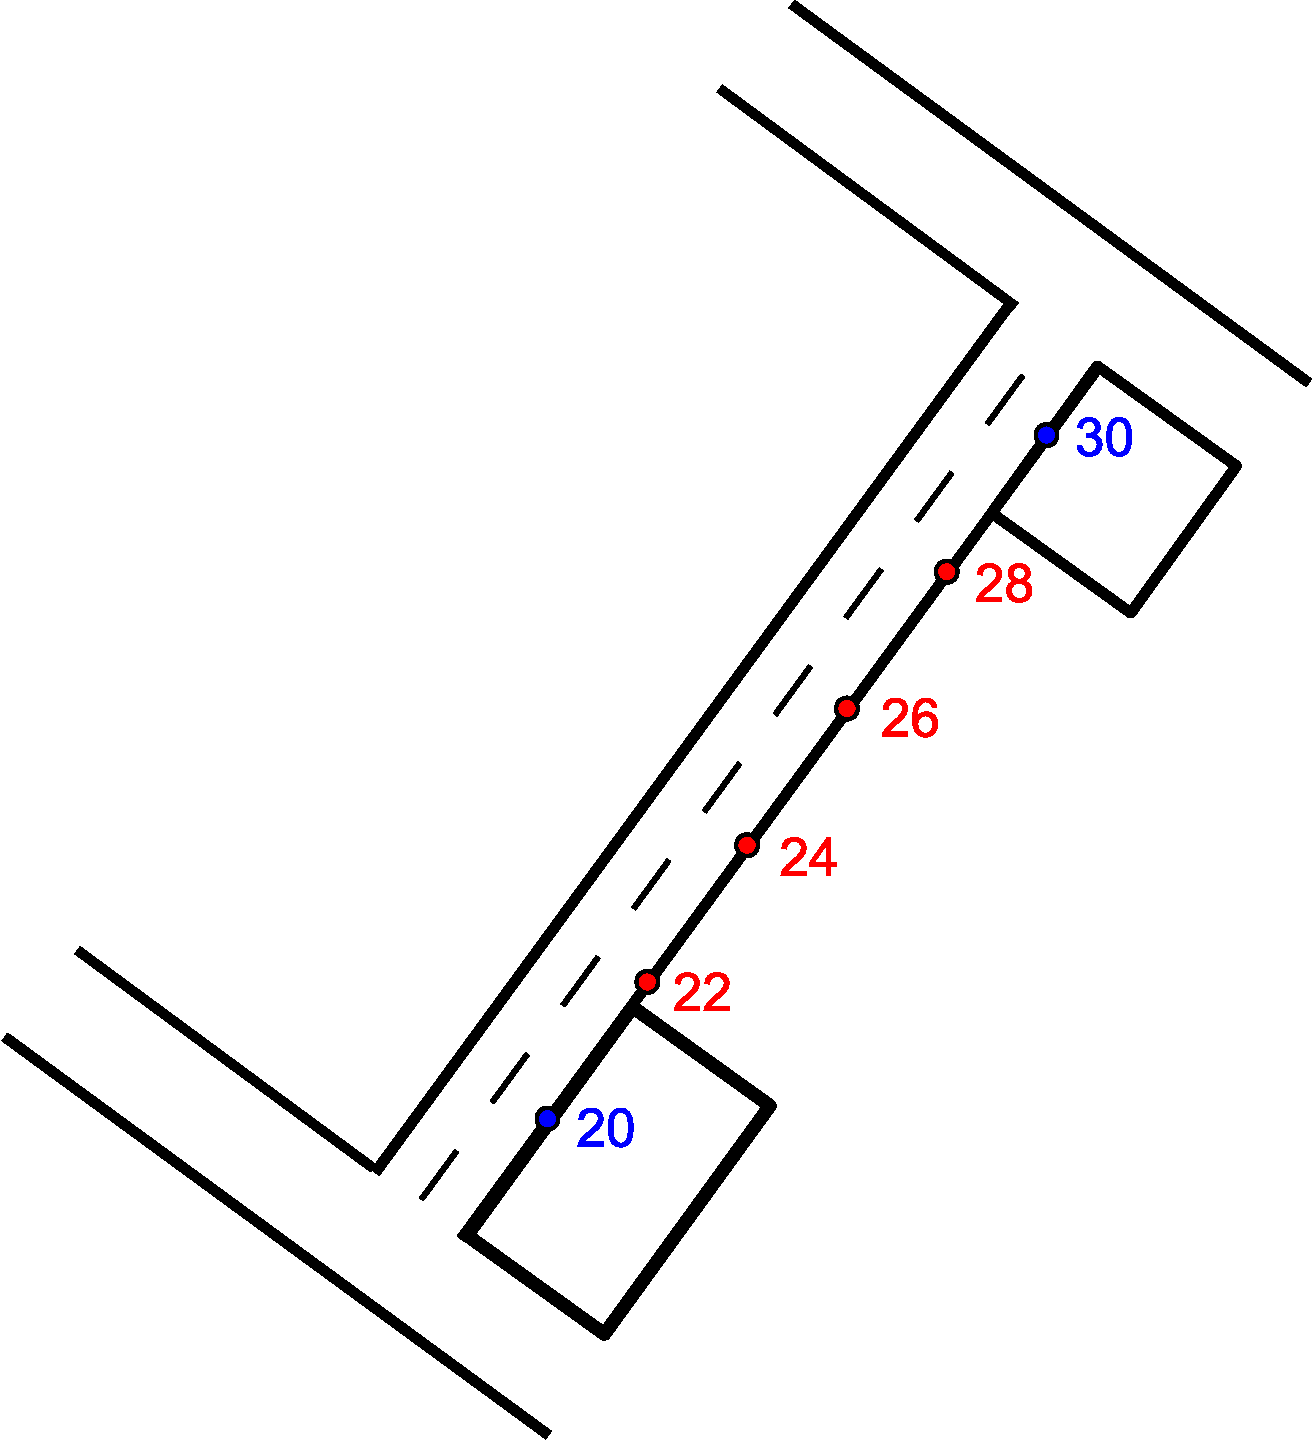
\includegraphics[width=.5\textwidth]{Fuentes_datos/Geocodificacion.pdf}
\caption{\small Interpolaci�n de direcciones. En azul, direcciones conocidas. En rojo, direcciones interpoladas.}
\label{Fig:Geocodificacion} 
\end{figure}

Esta pr�ctica, no obstante, no es del todo precisa, ya que asume que los edificios se encuentran equiespaciados, y por tanto son del mismo tama�o todos ellos, lo cual no sucede en la pr�ctica.  Adem�s de ello, el proceso presenta otras consideraciones particulares, tales como el hecho de que no en todos los pa�ses se sigue un mismo sistema de asignaci�n de direcciones postales, teniendo cada uno el suyo propio, que puede diferir en mayor o menor medida de lo que podr�a considerarse un sistema est�ndar. El supuesto habitual en que las direcciones pares se sit�an a un lado de la calle y las impares al lado contrario no resulta siempre cierto.

Otro aspecto a tener en cuenta es que el edificio se�alado con una direcci�n dada se identifica con una coordenada puntual, pero realmente ocupa una superficie \cite{WikipediaGeocoding}. Si esta es grande, puede presentar incluso varios puntos de acceso al mismo (o incluso accesos por varias calles distintas), con lo que la informaci�n que se recoge al geocodificar dicho edificio puede ser imprecisa e insuficiente.

Por todo ello, la interpolaci�n de direcciones permite una aproximaci�n v�lida para muchos usos, pero en aquellos casos en los que se requiera m�s precisi�n no pueden emplearse estas direcciones con total seguridad, ya que la exactitud de las coordenadas asociadas por el proceso de interpolaci�n puede variar notablemente seg�n sea la propia configuraci�n de los distintos edificios.

\subsection{Fotogrametr�a}\label{Fotogrametria}

\index{Fotogrametr�a}

Un caso particular de digitalizaci�n lo encontramos en la \emph{fotogrametr�a}. En la definici�n cl�sica de \cite{Bonneval1972Eyrolles}, esta se define como la t�cnica para estudiar y definir con precisi�n la forma, dimensiones y posici�n en el espacio de un objeto cualquiera, utilizando medidas realizadas sobre una o varias fotograf�as. Esta definici�n no limita el alcance de la fotogrametr�a al �mbito de lo geogr�fico, y se utilizan sus principios en campos tales como la arqueolog�a o la documentaci�n de obras y monumentos, empleando para ello fotograf�as no a�reas, sino terrestres. Es la denominada \emph{fotogrametr�a terrestre}. No obstante, la rama de inter�s para este libro es la de la \emph{fotogrametr�a a�rea}, cuya base de trabajo tradicional son las fotograf�as a�reas.

Esta clase de fotogrametr�a viene, pues, ligada �ntimamente a los inicios de la teledetecci�n, cuando los sensores modernos que hemos estudiado antes en este mismo cap�tulo no se hab�an desarrollado, y los existentes (b�sicamente c�maras fotogr�ficas especialmente adaptadas a la toma de fotograf�as de tipo cartogr�fico) se montaban a bordo de aviones. Es por esta raz�n que tradicionalmente existe una conexi�n indudable entre ambas materias, no existiendo una frontera clara entre ambas, y se consideran en ocasiones como t�rminos id�nticos que hacen referencia la disciplina global de obtenci�n de im�genes y tratamiento de estas.

Hist�ricamente, el t�rmino \emph{teledetecci�n} aparece con posterioridad, una vez que las t�cnicas de toma de im�genes avanzan y dan un gran salto cualitativo con la aparici�n de las im�genes satelitales y los sensores electro--�pticos que ya conocemos. Algunos autores engloban la fotogrametr�a dentro de la teledetecci�n, mientras que otros se refieren con el termino teledetecci�n a las tecnolog�as m�s actuales y las consideran disciplinas distintas aunque muy relacionadas. Junto con la fotogrametria a�rea aparece la fotogrametr�a espacial, encargada de operar sobre im�genes de sat�lite bajo unos principios similares.

Dentro de este libro entenderemos por teledetecci�n todo el conjunto de t�cnicas y operaciones de obtenci�n de im�genes (que ya conocemos), as� como las de tratamiento y posterior extracci�n de resultados a partir de estas (que iremos viendo en otros cap�tulos), obteni�ndose estos resultados sin necesidad de establecer contactos con los objetos a estudiar, como corresponde a la definici�n dada en el apartado correspondiente. Dentro de ese conjunto de operaciones que nos llevan desde las im�genes a los resultados, entendemos como parte de la fotogrametr�a aquellas que tienen relaci�n con la acepci�n original del t�rmino, es decir, aquellas que derivan de la medici�n de elementos.

La denominaci�n, no obstante, no es tan relevante, y s� lo es sin embargo comprender la importancia de ambas, particularmente dentro de este cap�tulo como t�cnicas de producci�n cartogr�fica. 

En lo que respecta a la fotogrametr�a, el proceso de \emph{restituci�n} es el que interesa principalmente para el contenido de este cap�tulo, pues ofrece como resultado nuevas capas de datos tanto bidimensionales como, especialmente, tridimensionales. As�, pueden obtenerse tanto las capas vectoriales digitalizadas que ve�amos por ejemplo en el apartado \ref{Digitalizacion_manual}, como directamente Modelos Digitales de Elevaciones a partir de im�genes.\index{Restituci�n}

En realidad, los procesos de digitalizaci�n que ya hemos visto son tambi�n parte de la fotogrametr�a digital, y es habitual encontrarlos en los textos al uso sobre esta. Tambi�n lo son los procesos de rectificaci�n que se han citado en su momento, y que analizaremos en detalle m�s adelante en el cap�tulo \ref{Procesado_imagenes}. Como puedes ver, todas las t�cnicas est�n sumamente relacionadas, y las divisiones que hacemos pueden ser unas u otras en funci�n del enfoque que se d� para su estudio

Todas estas operaciones se llevan a cabo con una \emph{estaci�n fotogram�trica}, que comprende las herramientas necesarias para llevar estas a cabo (algunas, como los esc�neres, ya las conocemos). En funci�n del tipo de herramientas y t�cnicas distinguimos los siguientes tipos de fotogrametr�a, que representan a su vez la evoluci�n de la disciplina.\index{Estaci�n fotogram�trica}

\begin{itemize}
	\item Fotogrametr�a anal�gica. Basada en mediciones y procedimientos sobre im�genes anal�gicas
	\item Fotogrametr�a anal�tica. Basada en formulaciones matem�ticas y t�cnicas computacionales, permite obtener grandes precisiones.
	\item Fotogrametr�a digital. Basada en el trabajo con im�genes digitales dentro de un entorno computerizado.
\end{itemize}

El inter�s principal desde el punto de vista de los SIG es en la fotogrametr�a digital, ya que existe una gran relaci�n entre estos y las aplicaciones empleadas en dicho tipo de fotogrametr�a. Es en esta en la que pueden englobarse los procesos de digitalizaci�n que ya hemos visto, y no en las restantes formas m�s antiguas de fotogrametr�a. En la fotogrametr�a digital, la estaci�n fotogram�trica se articula sobre un ordenador en el cual se llevan a cabo los distintos procesos, no existiendo operaciones externas al mismo. As�, las im�genes se manejan dentro del ordenador y se visualizan a trav�s de �l, y la generaci�n de nueva cartograf�a tambi�n se produce de forma digital.

Esto no es muy diferente de lo que ve�amos en el caso de la digitalizaci�n en pantalla algunas paginas atr�s, pero el trabajo fotogram�trico engloba otros procesos adem�s de los que ya hemos visto. Uno de ellos es la generaci�n directa de cartograf�a de elevaciones, para la cual se requiere que el equipo empleado disponga de algunos elementos adicionales. Es decir, la estaci�n fotogram�trica digital es m�s compleja que un simple ordenador, un dispositivo de marcado (un rat�n) y un SIG, que eran los requisitos b�sicos para digitalizar en pantalla una imagen.

Una estaci�n fotogram�trica digital ha de tener, por ejemplo, capacidad para generar visualizaciones con sensaci�n de profundidad a partir de pares de im�genes, que son las que permiten la posterior digitalizaci�n de los elementos con sus elevaciones correspondientes. Los principios en los que se basan este tipo de visualizaciones son los mismos empleados en la fotogrametr�a no digital, fundamentados en la visi�n estereosc�pica. \index{Par estereosc�pico}

La visi�n tridimensional en el ser humano se basa en el hecho de que la imagen que ve cada ojo es ligeramente distinta a la del otro, lo cual permite al cerebro extraer informaci�n volum�trica y generar una verdadera visi�n tridimensional. En el caso de la fotogrametr�a, si en lugar de utilizar una �nica imagen a�rea o de sat�lite empleamos dos, cada una de ellas tomada desde un punto distinto, resulta posible recrear el efecto que ambas im�genes tendr�an para la reconstrucci�n tridimensional de la escena, y <<enga�ar>> al cerebro del observador para que este pueda observar la escena con volumen y profundidad.

Cuando se emplean im�genes de sat�lite, los pares se pueden obtener con aquellas plataformas y sensores que permiten variar el �ngulo de visi�n, de modo que en la misma pasada del sat�lite se toman im�genes de una zona desde distintos puntos. El sensor toma una imagen cenital y posteriormente, una vez ha superado la zona en su recorrido, toma una segunda imagen mirando <<hacia atr�s>>, la cual, combinada con la primera, permite el levantamiento del terreno y la realizaci�n de los procesos fotogram�tricos (Figura \ref{Fig:Par_estereo_satelite}).

\begin{figure}[!hbt]
\centering
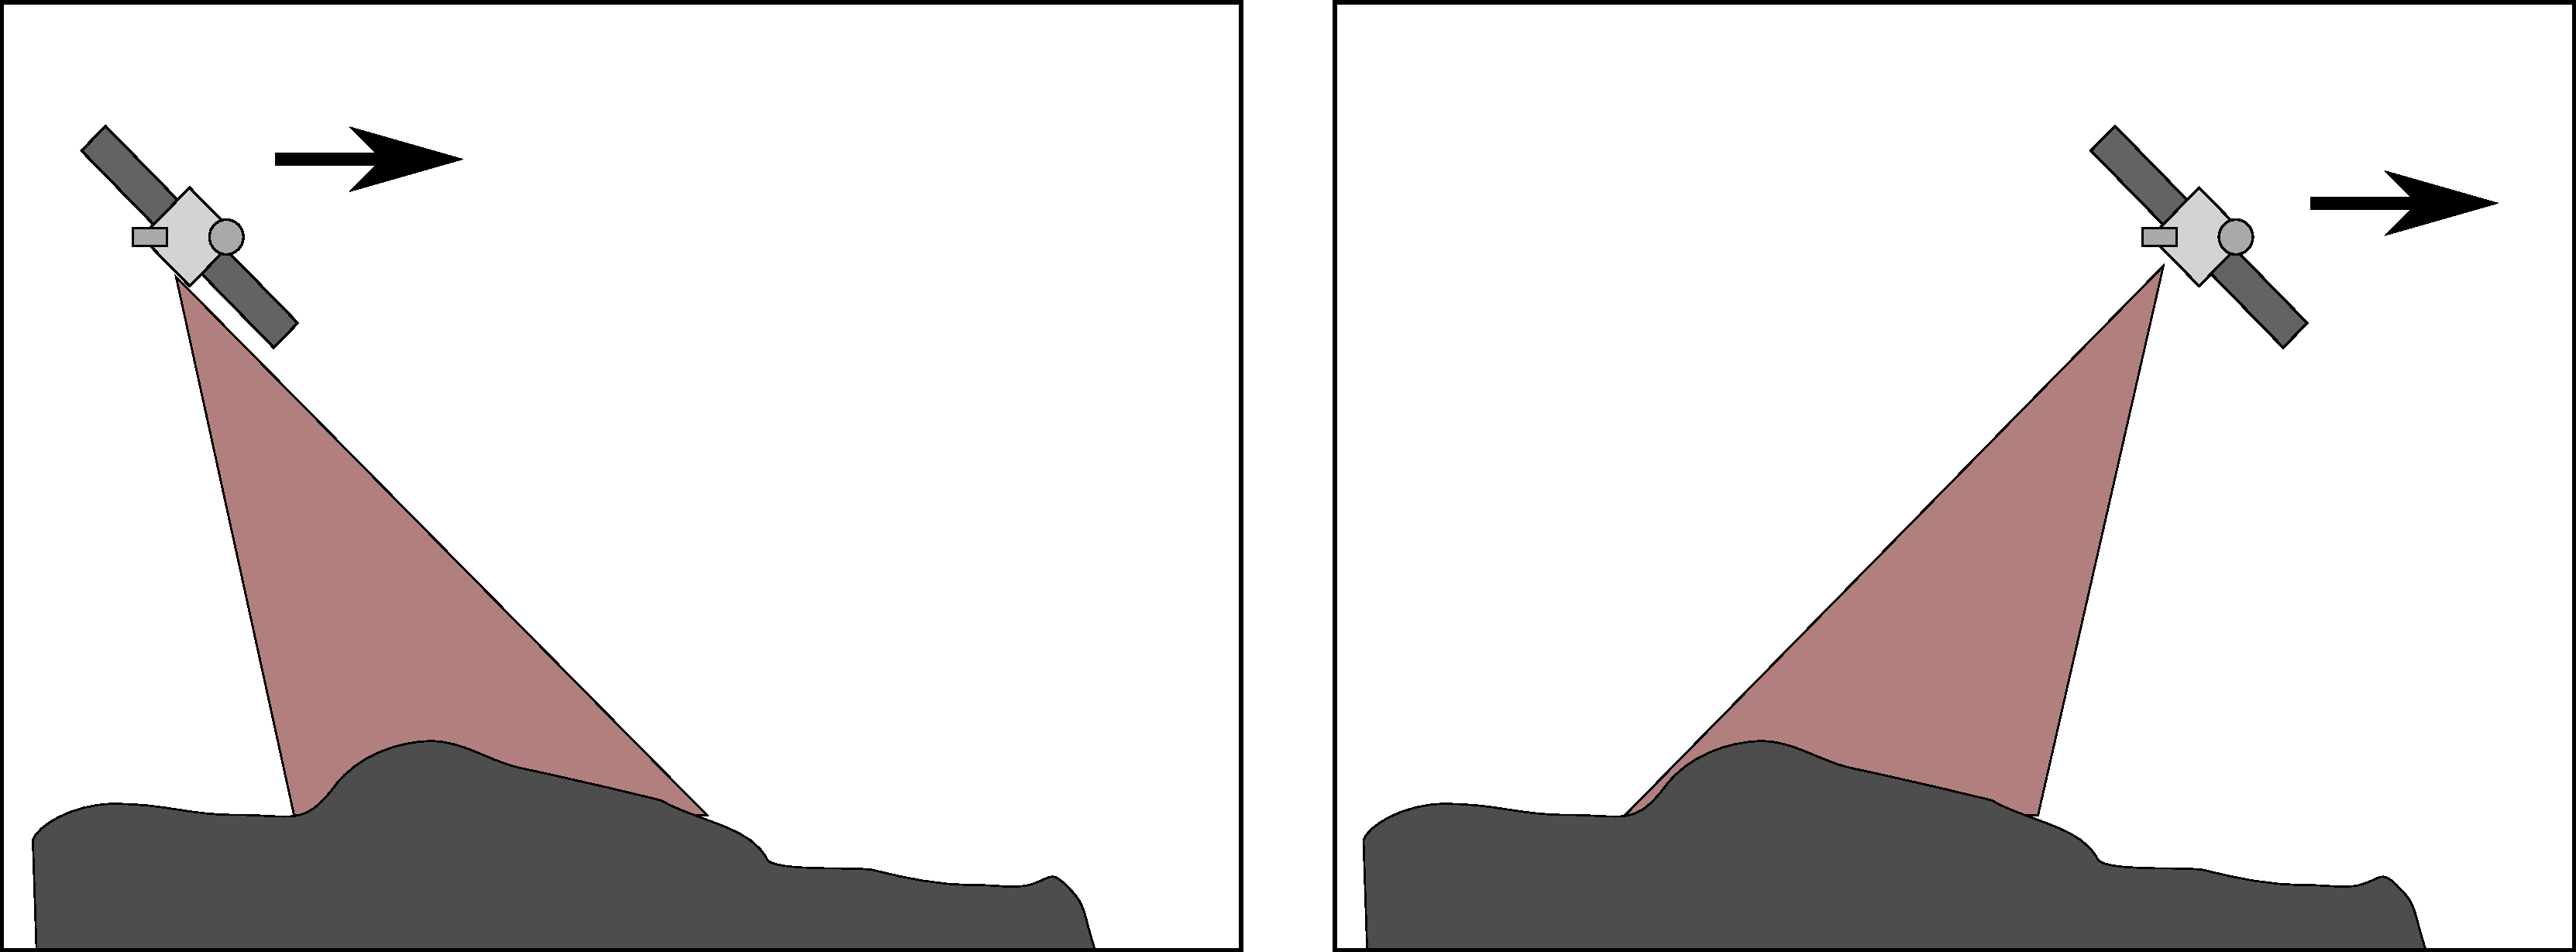
\includegraphics[width=.85\textwidth]{Fuentes_datos/Par_estereo_satelite.pdf}
\caption{\small Toma de pares de im�genes estereos�picas desde un sat�lite, mediante variaci�n del �ngulo de visi�n.}
\label{Fig:Par_estereo_satelite} 
\end{figure}

El sensor HRS que montan los sat�lites SPOT, o el sensor ASTER, ambos son capaces de tomar este tipo de im�genes. En la direcci�n Web \cite{webSPOTDEM} puede encontrarse informaci�n detallada sobre las cartograf�a de elevaciones generada a partir de pares de im�genes tomadas por el sat�lite SPOT, junto con algunas ilustraciones y animaciones explicativas al respecto. \index{SPOT}\index{ASTER}

Las formas de conseguir que el observador perciba la profundidad de la escena a partir de las im�genes son variadas, y van desde el uso de sencillos instrumentos �pticos o la generaci�n de anaglifos (im�genes que combinan la informaci�n del par estereosc�pico y que se han de observar con gafas con filtros distintos para cada ojo), hasta otras t�cnicas m�s complejas y elaboradas. En la fotogrametr�a no digital, el empleo de restituidores anal�ticos %como el mostrado en la figura \ref{Fig:Restituidor_analitico} 
ha sido la metodolog�a habitual. En la fotogrametr�a digital, este puede sustituirse por un equipo con dos monitores, cada uno de los cuales muestra una de las im�genes del par, y se emplean gafas especiales que son las encargadas de generar en el observador la sensaci�n de profundidad .\index{Anaglifos}

%\begin{figure}
%\centering
%\includegraphics[width=.9\mycolumnwidth]{Fuentes_datos/Restituidor_analitico.png}
%\caption{\small Restituidor anal�tico.}
%\label{Fig:Restituidor_analitico} 
%\end{figure}

\begin{figure}
\centering
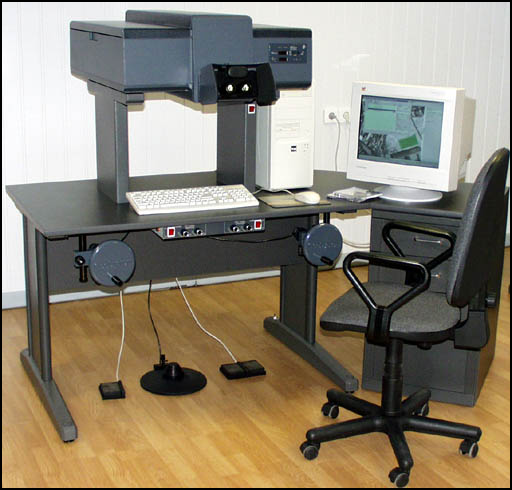
\includegraphics[width=.5\textwidth]{Fuentes_datos/Estacion_fotogrametrica_digital.png}
\caption{\small Estaci�n fotogram�trica digital.}
\label{Fig:Estacion_fotogrametrica_digital} 
\end{figure}

Adem�s de lo anterior, la estaci�n fotogram�trica digital dispone de perif�ricos espec�ficos tales como ratones 3D, o manivelas como las que presentan los restituidores anal�ticos, facilitando as� la adaptaci�n de los operarios a este tipo de estaci�n (Figura \ref{Fig:Estacion_fotogrametrica_digital}).

Por �ltimo el software que implementan, y que es el encargado de representar las im�genes y acoger el proceso de digitalizaci�n, suele ser espec�fico, y es frecuente que se distribuya como parte de toda una estaci�n fotogram�trica compuesta por los elementos rese�ados anteriormente. Algunos SIG incorporan progresivamente capacidades adaptadas de este tipo de programas, pero por el momento la labor fotogram�trica queda reservada para este tipo de aplicaciones espec�ficas, siendo el SIG tan solo un beneficiario directo de sus productos.

Para el lector interesado en saber m�s acerca de los distintos elementos de la fotogrametr�a, obras como  \cite{Lerma2002UPV} o \cite{Brito2002IME} son recomendables, esta �ltima disponible de forma libre. En la direcci�n Web \cite{webFotogrametriaUNEX} puede encontrarse otra excelente referencia libre en dos tomos sobre fotogrametr�a anal�tica y digital.

\subsection{Calidad de la digitalizaci�n}\label{Condiciones_digitalizacion}

\index{Digitalizaci�n!calidad}

Uno de los aspectos m�s importantes del proceso de digitalizaci�n es la calidad del resultado obtenido, que debe tratar de ser lo m�s cercano posible a la calidad original de la informaci�n que se digitaliza, es decir, del mapa o imagen original. Independientemente de la precisi�n del equipo utilizado o la habilidad y experiencia del operario, la digitalizaci�n no es por completo perfecta, conteniendo siempre ciertas deficiencias y errores. 

Adem�s de los errores que puedan incorporarse en las distintas fases del proceso de digitalizaci�n (sea este del tipo que sea), hay que considerar que las fuentes originales a digitalizar tambi�n pueden incluir los suyos propios. As�, el proceso de escaneado puede incorporar distorsiones geom�tricas, pero es posible que el mapa o fotograf�a a�rea de partida tambi�n presente alguna distorsi�n como consecuencia de su deterioro, m�s patente cuanto m�s antigua sea esta. 

La informaci�n contenida en el documento cartogr�fico puede tambi�n contener elementos problem�ticos de cara a obtener un producto de calidad, que pueden ir desde l�neas borradas total o parcialmente a manchas en el propio mapa derivadas de su uso habitual \cite{Heywood1998Longman}.

Dentro de los errores que aparecen como consecuencia de la digitalizaci�n en s�, un tipo importante de ellos son las discrepancias y coincidencias imperfectas entre las distintas entidades, tal como las que se muestran en la figura \ref{Fig:Imprecisiones_digitalizacion}

\begin{figure}[!hbt]   
\centering
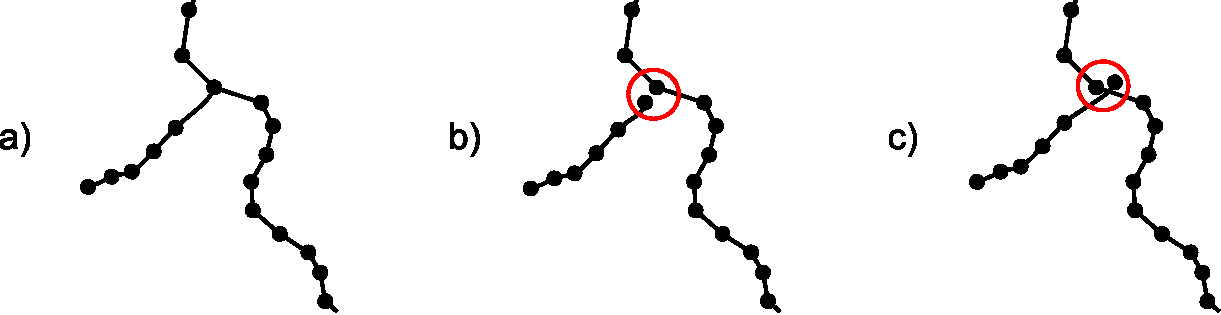
\includegraphics[width=.8\textwidth]{Fuentes_datos/Imprecisiones_digitalizacion.pdf}
\caption{\small Errores derivados del proceso de digitalizaci�n. a) Versi�n correcta, con nodos coincidentes. b) y c) Versiones con errores que causan una falsa desconexi�n entre las l�neas.}
\label{Fig:Imprecisiones_digitalizacion} 
\end{figure}

Estas imprecisiones son causantes de numerosos problemas, tales como la aparici�n de pol�gonos esp�reos en las operaciones de solape entre capas vectoriales, que veremos en el cap�tulo \ref{Operaciones_geometricas}.\index{Pol�gono!espureo}

Debido a esto, las capacidades de edici�n de los SIG incorporan funcionalidades que permiten evitar estos errores en el momento de la digitalizaci�n, ayudando al operario en su tarea y permiti�ndole alcanzar una exactitud y precisi�n imposible de lograr sin estas funcionalidades. Entre ellas, es especialmente importante el establecimiento de tolerancias y ajuste autom�tico en funci�n de ellas (esto se conoce con el t�rmino ingles \emph{snapping}), que ayudan a garantizar la coincidencia entre los distintos v�rtices. \index{Snapping}

De este modo, pol�gonos adyacentes o lineas que se cortan en un punto dado lo hacen con total exactitud. Dichos pol�gonos comparten exactamente el mismo lado con las mismas coordenadas exactas, o se cruzan en el mismo e id�ntico punto, y no �nicamente pasan por un punto cercano (pero distinto) definido con la precisi�n con la que el operador haya podido ajustar ambas entidades visualmente. La coincidencia no es solo visual, sino num�rica. La figura \ref{Fig:Snapping} muestra un ejemplo de la utilizaci�n de \emph{snapping} en un proceso de digitalizaci�n.

\begin{figure}
\centering
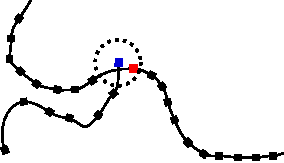
\includegraphics[width=.4\textwidth]{Fuentes_datos/Snapping.pdf}
\caption{\small Ajuste autom�tico mediante tolerancia(\emph{snapping}). El nodo azul representa el nodo en edici�n. La tolerancia de enlace queda marcada por el circulo punteado. Puesto que el nodo rojo de la l�nea preexistente se encuentra dentro de esa tolerancia, al a�adir el nuevo nodo (azul), este autom�ticamente se situar� en las coordenadas del nodo rojo, garantiz�ndose as� la coincidencia.}
\label{Fig:Snapping} 
\end{figure}

Mediante estas funcionalidades, el operador simplemente selecciona un punto, y el sistema digitalizador lo desplaza para que coincida con el punto existente m�s cercano, siempre que se encuentre a menos distancia que la tolerancia establecida de antemano.

El hecho de que exista una completa coincidencia es especialmente importante cuando la capa vectorial que se digitaliza contiene informaci�n topol�gica. La topolog�a exige que la coincidencia sea correcta y defina perfectamente la relaci�n entre las entidades. Para los ejemplos b) y c) de la figura \ref{Fig:Imprecisiones_digitalizacion}, las l�neas no est�n conectadas ya que no existe coincidencia en el nodo. Si los puntos est�n suficientemente cercanos, puede <<parecer>> que son coincidentes, pero el SIG no los detectar� como tales y no se podr� llevar a cabo ning�n an�lisis topol�gico con esas l�neas (por ejemplo, suponiendo que representan v�as de comunicaci�n y se quiere hacer un an�lisis de redes con ellas).

La digitalizaci�n de entidades en caso de querer recoger la topolog�a\index{Topolog�a} de las mismas debe obedecer una serie de reglas, a saber\cite{GrassDigitizing}:

\begin{itemize}
	\item Las l�neas deben cruzarse en nodos, en caso de que exista relaci�n (conexi�n) entre ellas.
	\item Las lineas que coinciden en un nodo com�n deben coincidir exactamente. Las funciones de \emph{snapping} se han de utilizar por ello durante la digitalizaci�n.
	\item Los lados comunes de los pol�gonos deben digitalizarse una �nica vez.
	\item Las �reas deben ser cerradas (el primer punto ha de coincidir exactamente con el �ltimo). Las funciones de \emph{snapping} o el cierre autom�tico de l�neas (asignar sistem�ticamente al �ltimo punto del contorno del pol�gono las coordenadas del primero) deben emplearse para ello.
\end{itemize}

Todos aspectos relativos a la calidad de datos, entre los cuales se incluyen las aspectos relativos a los errores del proceso de digitalizaci�n, se tratan con mayor profundidad en el cap�tulo \ref{Calidad_datos}.\index{Datos!calidad}


\section{GPS}\label{GPS}

Uno de los hitos en la aparici�n de nuevas fuentes de datos geogr�ficos es la aparici�n de los \emph{Sistemas Globales de Navegaci�n por Sat�lite} (GNSS)\footnote{\extr{Global Navigation Satellite System}}, que permiten la obtenci�n de coordenadas geogr�ficas de un modo inmediato, con las consecuencias que esto tiene para su uso en actividades como la elaboraci�n de cartograf�a.\index{GNSS}\index{GPS}

En esencia, un GNSS es un sistema que permite conocer en todo momento y en cualquier punto del globo la localizaci�n exacta de dicho punto con un margen de error del orden de unos pocos metros o menos. Para ello, se basan en el env�o de se�ales entre un dispositivo situado en el punto concreto y una red de sat�lites, pudiendo establecerse la posici�n exacta mediante las caracter�sticas de dicha transmisi�n.

El ejemplo m�s extendido de un GNSS es el Sistema de Posicionamiento Global (Global Positioning System, o GPS)\footnote{El nombre completo del sistema es NAVSTAR--GPS (NAVigation SysTem And Ranging - Global Position System)}, originalmente puesto en funcionamiento por el Departamento de Defensa de los Estados Unidos. Actualmente, este es el �nico GNSS completamente operativo, aunque existen otros tales como el GLONASS ruso, el COMPASS chino o el \emph{Galileo} europeo, cuyo funcionamiento completo est� previsto a corto plazo. \index{GLONASS}\index{Galileo}\index{COMPASS}

\subsection{Fundamentos del sistema GPS}

El sistema GPS se divide en tres subsistemas o \emph{segmentos}:

\begin{itemize}
	\item Segmento espacial. Lo componen los sat�lites de la constelaci�n GPS (un total de 27, siendo 24 de ellos operativos y 3 de reserva), con los cuales se comunican las unidades receptoras, y en funci�n de los cuales puede triangularse la posici�n actual de estas.
	\item Segmento de control. Lo forman un conjunto de estaciones terrestres que controlan el funcionamiento de los sat�lites, pudiendo enviar se�ales a estos para modificar su comportamiento.
	\item Segmento de usuarios. Lo conforman los receptores GPS y todos los dispositivos que hacen uso de la se�al de los sat�lites para el c�lculo de posiciones.
\end{itemize}

\index{Segmentos!del sistema GPS}

Los sat�lites del segmento espacial emiten una se�al compleja cuyo contenido puede dividirse esencialmente en dos bloques de informaci�n:

\begin{itemize}
	\item Se�ales empleadas para el c�lculo de distancias. Estas incluyen dos c�digos: P(Precise) y C/A (Coarse/Aquisition). El segundo de ellos es el empleado habitualmente, ya que el primero se encuentra encriptado y est� pensado para uso militar, mientras que el C/A esta disponible para todos los usuarios.
	\item Mensajes de navegaci�n. Estos informan de la posici�n orbital del sat�lite (conocida como \emph{efem�ride}), y pueden asimismo contener informaci�n adicional referente al segmento espacial.
\end{itemize}

\index{Efem�ride}

Las se�ales para el c�lculo de distancias (en la terminolog�a GPS estas distancias se conocen como \emph{pseudodistancias}) se env�an mediante una onda portadora conocida como L1, correspondiente a una frecuencia de 1575,42 MHz . El c�digo P se env�a adem�s en una segunda portadora denominada L2, con una frecuencia de 1227,60 MHz.\index{Pseudodistancias}

El funcionamiento del sistema se basa en la triangulaci�n de la posici�n mediante las se�ales procedentes de un cierto n�mero de los sat�lites. Esta posici�n se calcula no �nicamente en sus coordenadas \emph{x} e \emph{y}, sino tambi�n en \emph{z}, es decir en elevaci�n. El sistema GPS emplea como sistema geod�sico de referencia el WGS84 \cite{WGS84}. La precisi�n en el c�lculo de la elevaci�n es menor que la correspondiente a las restantes coordenadas, aunque tambi�n es de utilidad y puede emplearse en aplicaciones que van desde levantamientos y replanteos a usos en tiempo real como el c�lculo de elevaci�n en vuelos \cite{Graas1991Navigation}.\index{WGS84}

La posici�n de los sat�lites es conocida en todo momento, y los propios sat�lites informan de ella a los receptores a trav�s de los mensajes de navegaci�n. En base a esas posiciones orbitales, el proceso de triangulaci�n que se lleva a cabo en el sistema GPS no se basa en el trabajo con �ngulos, sino con distancias.

El c�lculo de la distancia puede realizarse utilizando la informaci�n de las se�ales (los c�digos C/A o P), o bien empleando las propias portadoras. El primer m�todo es m�s sencillo y r�pido, ya que no es necesario que el receptor <<escuche>> la se�al durante un periodo prolongado de tiempo, lo cual s� es necesario en el segundo, como a continuaci�n veremos. 

En el caso de emplear la portadora, se mide el desfase entre esta y una se�al generada por el receptor, lo cual permite calcular una parte de la distancia (la que es menor que la longitud de onda de la se�al). La distancia total es igual a esta parte calculada m�s un numero entero de veces la longitud de onda. El valor de este numero entero es, no obstante, desconocido. Su c�lculo se conoce como \emph{resoluci�n de la ambig�edad} (AR), y requiere escuchar la se�al del sat�lite durante un cierto tiempo para recopilar datos suficientes que permitan el c�lculo del valor antedicho.\index{Resoluci�n!de la ambig�edad}

As�, la resoluci�n de la ambig�edad es la que hace necesario un tiempo de \emph{inicializaci�n} de la unidad, con objeto de conocer esa constante en el desfase. Si la unidad pierde contacto con el sat�lite, es necesario de nuevo proceder a la resoluci�n de las ambig�edades, quedando el receptor inoperativo durante ese periodo de tiempo. M�s detalles sobre la resoluci�n de la ambig�edad en el sistema GPS puede encontrarse en \cite{Torrecillas1998Mapping}.

Puesto que la velocidad a la que la se�al se desplaza es muy elevada, se requieren relojes muy precisos para poder medir con precisi�n los tiempos tan cortos que tarda dicha se�al en recorrer la distancia entre sat�lite y receptor. A bordo de los sat�lites se montan relojes at�micos de muy alta precisi�n, pero las unidades receptoras no disponen de relojes tan precisos. Es por este motivo que, como veremos, han de introducirse correcciones y c�lculos adicionales con el fin de obtener mayores precisiones en la medida del tiempo.

Si el receptor es capaz de establecer comunicaci�n con tres sat�lites, dispone ya de informaci�n suficiente para conocer su posici�n $(x,y)$ como intersecci�n de las esferas centradas en cada uno de dichos sat�lites y con radio la distancia existente entre este y el receptor. Con cuatro sat�lites se puede ya obtener la posici�n $(x,y,z)$.

Un n�mero mayor de sat�lites (cuatro al menos) es necesario, no obstante, para eliminar las imprecisiones debidas a los distintos elementos implicados, y se emplean habitualmente modelos m�s complejos que utilizan los datos de m�ltiples sat�lites y efect�an correcciones en funci�n de ellos. Las deficiencias de los relojes que emplean los receptores pueden corregirse mediante la utilizaci�n de nuevos sat�lites, que permiten calcular con exactitud el tiempo, variable de gran importancia en el proceso y sin la cual no se pueden obtener precisiones elevadas.

Los receptores actuales est�n preparados para trabajar con un n�mero m�ximo de sat�lites habitualmente igual a 12, por lo que en todas circunstancias el receptor trata de localizar siempre el mayor n�mero posible de sat�lites con objeto de lograr una mayor precisi�n.

El dise�o de la red de sat�lites est� pensado para garantizar que en cualquier punto de la superficie terrestre y en cualquier momento, un receptor puede localizar el n�mero necesario de sat�lites para obtener con exactitud su precisi�n. La localizaci�n en la que se disponen los sat�lites con los que se establece comunicaci�n no es irrelevante, ya que condiciona la precisi�n del posicionamiento, afectando a lo que se conoce como \emph{diluci�n de la precisi�n} (DOP\footnote{Dilution of Precision}). Si los �ngulos de los sat�lites son grandes, la precisi�n que se obtiene es mayor que si estos son menores (Figura \ref{Fig:DOP}).\index{Dilution of Precision}

\begin{figure}
\centering
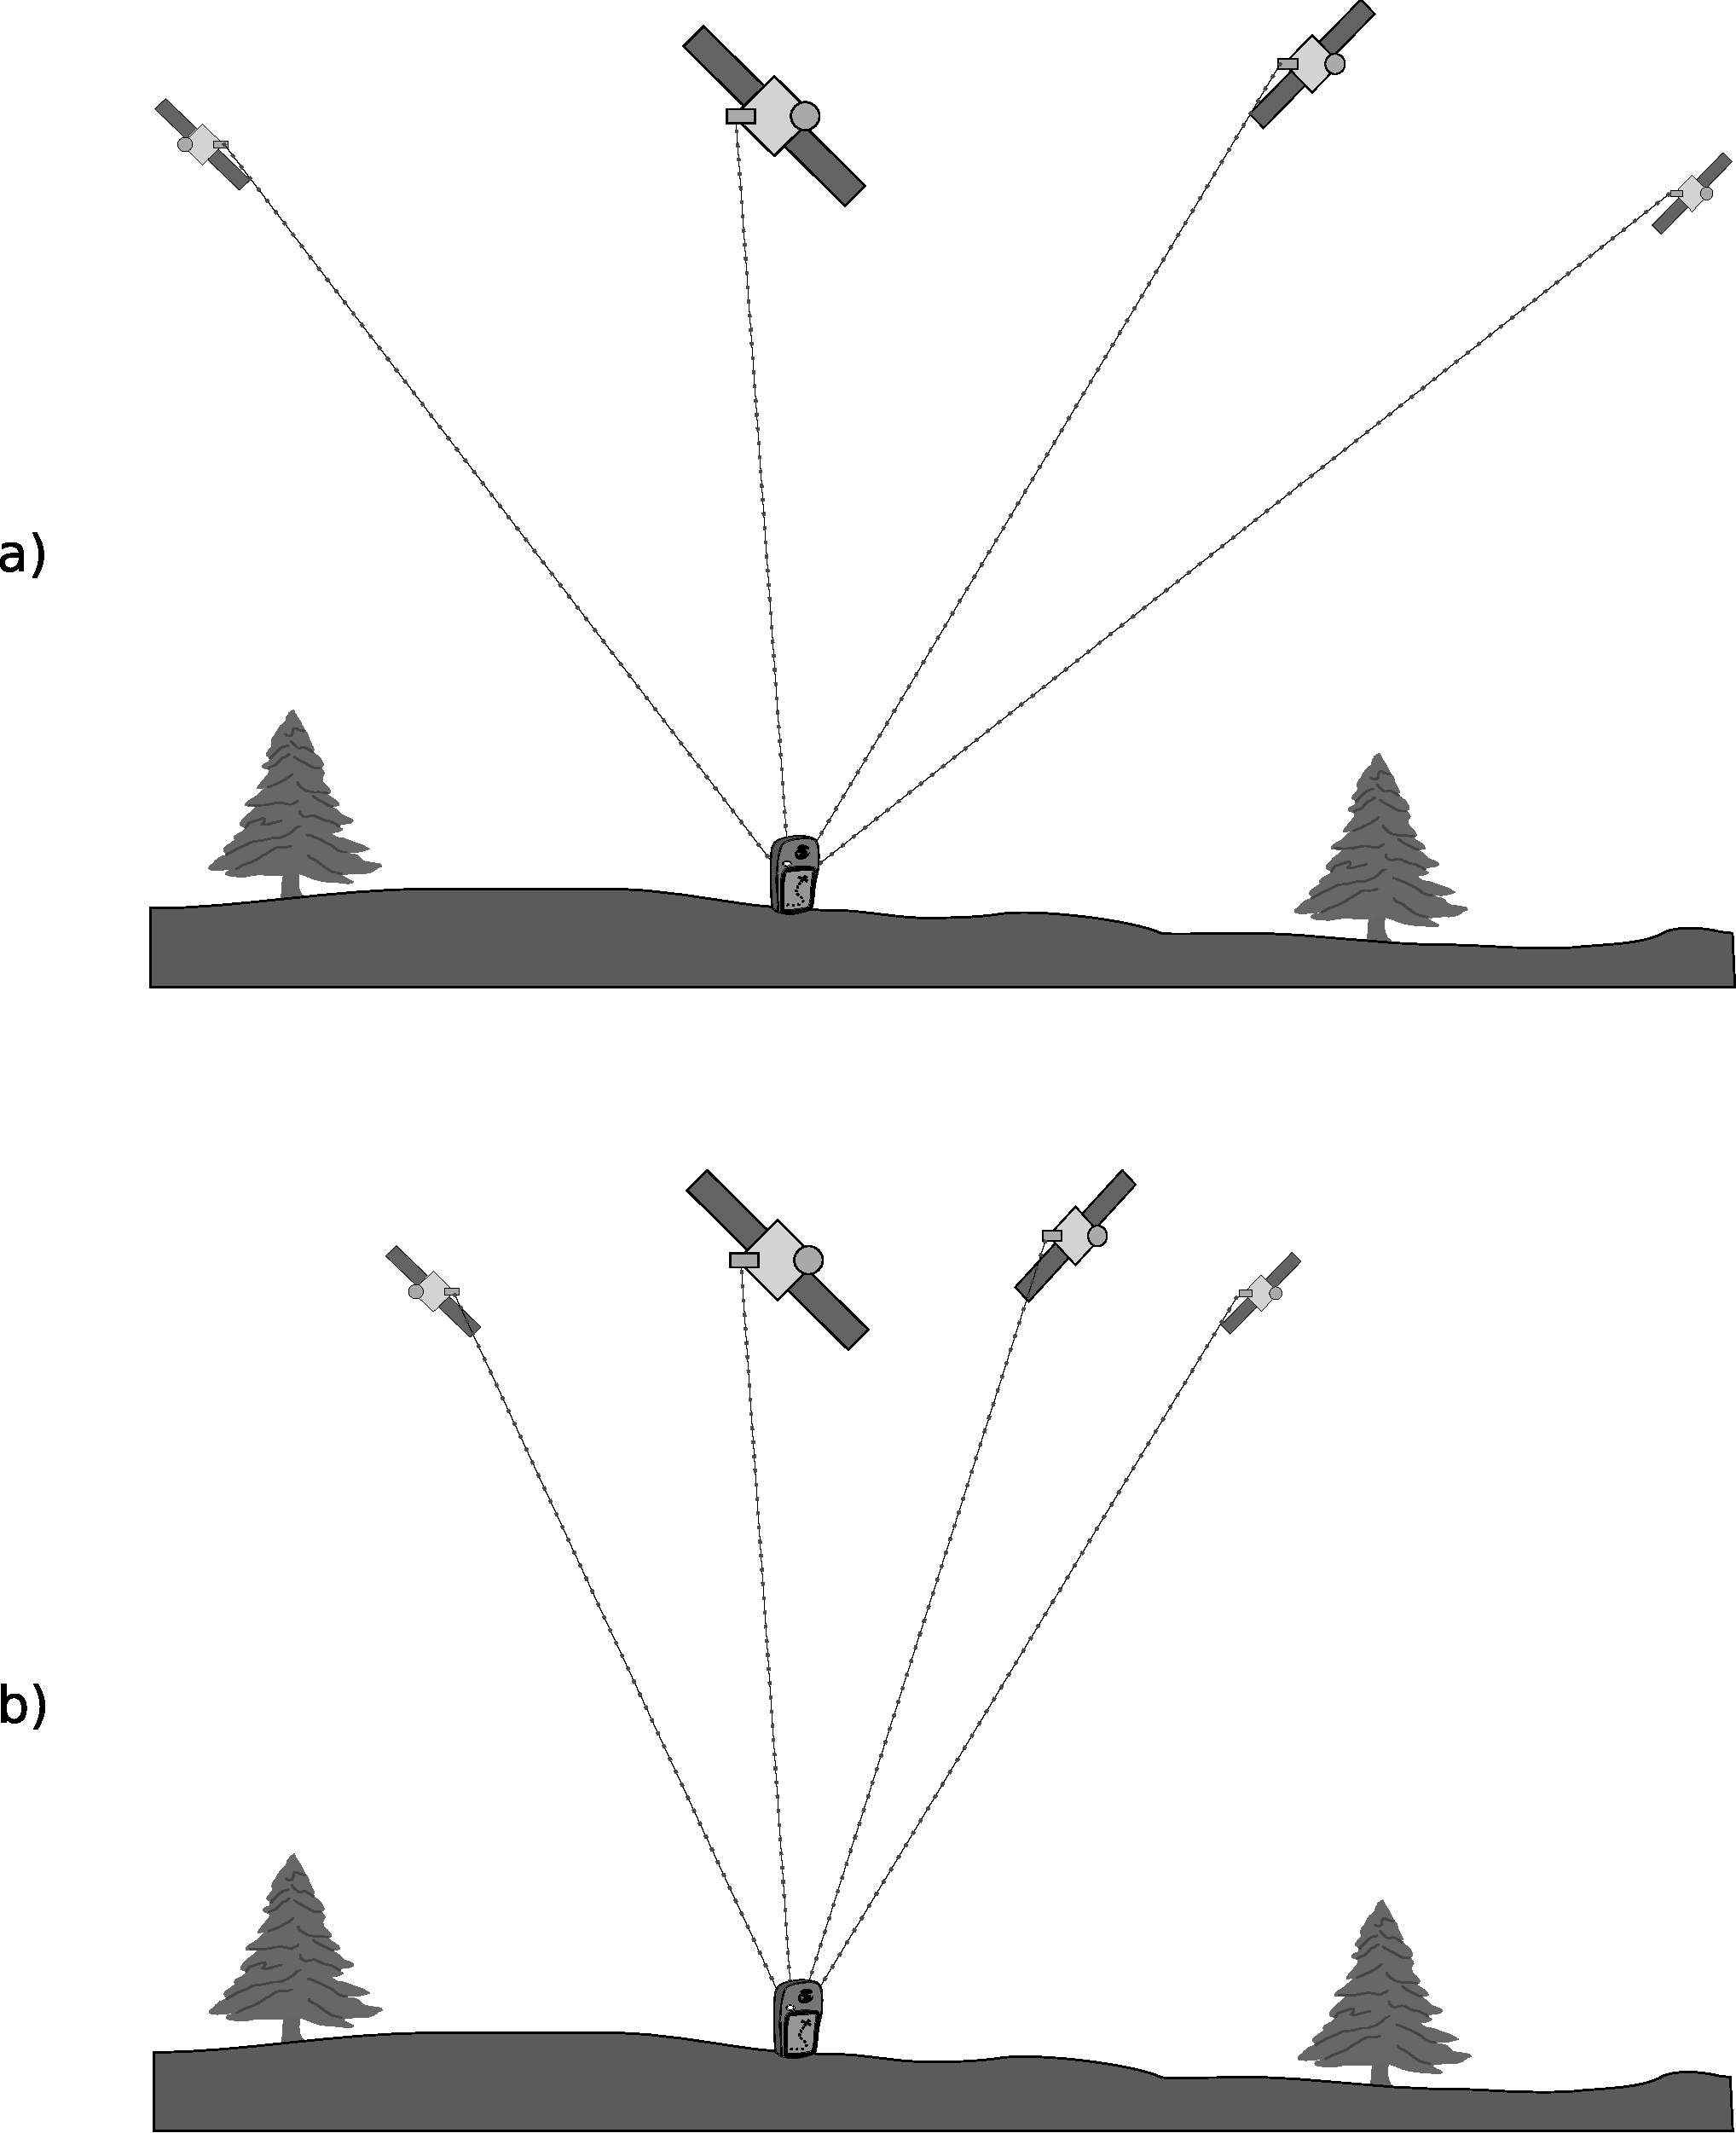
\includegraphics[width=.7\textwidth]{Fuentes_datos/DOP.pdf}
\caption{\small Diluci�n de la precisi�n. La geometr�a de los sat�lites en el ejemplo a) da una mayor precisi�n en el c�lculo de la posici�n del receptor que la del ejemplo b).}
\label{Fig:DOP} 
\end{figure}

Junto a esto, existen otras muchas fuentes de error en el sistema GPS, cada una de las cuales afecta a la precisi�n del mismo. Entre ellas, cabe destacar las siguientes:

\begin{itemize}
	\item Errores en la posici�n de los sat�lites.
	\item Errores por el rebote de la se�al en otros elementos tales como edificios, con anterioridad a alcanzar el receptor.
	\item Errores derivados del paso de la se�al por la atm�sfera. Al atravesar la ionosfera y la troposfera se genera un retraso por la alteraci�n que dicho paso produce sobre la se�al.
	\item Errores en la precisi�n de los relojes, ya mencionados.
	\item \emph{Disponibilidad selectiva}. Debido a su concepci�n como una herramienta militar, el departamento de Defensa de los Estados Unidos, propietario del sistema, introduc�a errores aleatorios en las se�ales, de tal forma que esta quedaba degradada y los usuarios civiles no pod�an obtener una precisi�n muy elevada. La disponibilidad selectiva fue eliminada en el a�o 2000.
\end{itemize}

\index{GPS!fuentes de error}

En conjunto, todos estos errores suman desviaciones apreciables, que sin embargo pueden corregirse con la aplicaci�n de t�cnicas adicionales, por ejemplo incorporando informaci�n adicional procedente de otros receptores. Una de estas t�cnicas es el denominado \emph{GPS diferencial}, pensado en origen para eliminar el error de la disponibilidad selectiva, aunque tambi�n eficaz para corregir una buena parte los restantes errores citados anteriormente.\index{GPS!diferencial}

Para la aplicaci�n del GPS diferencial se requiere no solo un receptor �nico (aquel del cual se quiere calcular su posici�n), sino tambi�n otro receptor fijo de referencia cuyas coordenadas se conocen con alta precisi�n. Este receptor fijo es, a su vez, un receptor de alta precisi�n y, adem�s de calcular su propia posici�n, emite informaci�n que las unidades receptoras pueden aprovechar para corregir sus mediciones. El receptor m�vil, l�gicamente, tiene que soportar este tipo de correcciones, para poder hacer uso de la se�al de la estaci�n de referencia.

Los datos que permiten llevar a cabo la correcci�n puede obtenerse en el receptor mediante radio, descargarse por Internet mediante una conexi�n inal�mbrica, o bien utilizar una constelaci�n de satelites adicional dedicada a elaborar y servir este tipo de datos.

La correcci�n puede realizarse fuera del propio receptor, a posteriori, utilizando software adecuado y los mismos datos de correcci�n que si se realiza la correcci�n en tiempo real.

El fundamento de este sistema es que los errores que afectan al receptor m�vil tambi�n afectan al de referencia. No obstante, la magnitud del error que afecta al receptor de referencia puede conocerse, ya que se conoce la coordenada exacta de este, y en base a eso puede eliminarse el error que afecta al receptor m�vil, asumiendo que ambos errores son de similar �ndole.

En la actualidad, aplicando estas t�cnicas de correcci�n diferencial, un GPS puede obtener precisiones del orden de 2 metros en latitud y longitud, y 3 en altitud\cite{wikipediaGPS}. Sin correcci�n diferencial, esta precisi�n es de unos 10--20 metros.

La figura \ref{Fig:DGPS} muestra un esquema del funcionamiento del GPS diferencial.

\begin{figure}
\centering
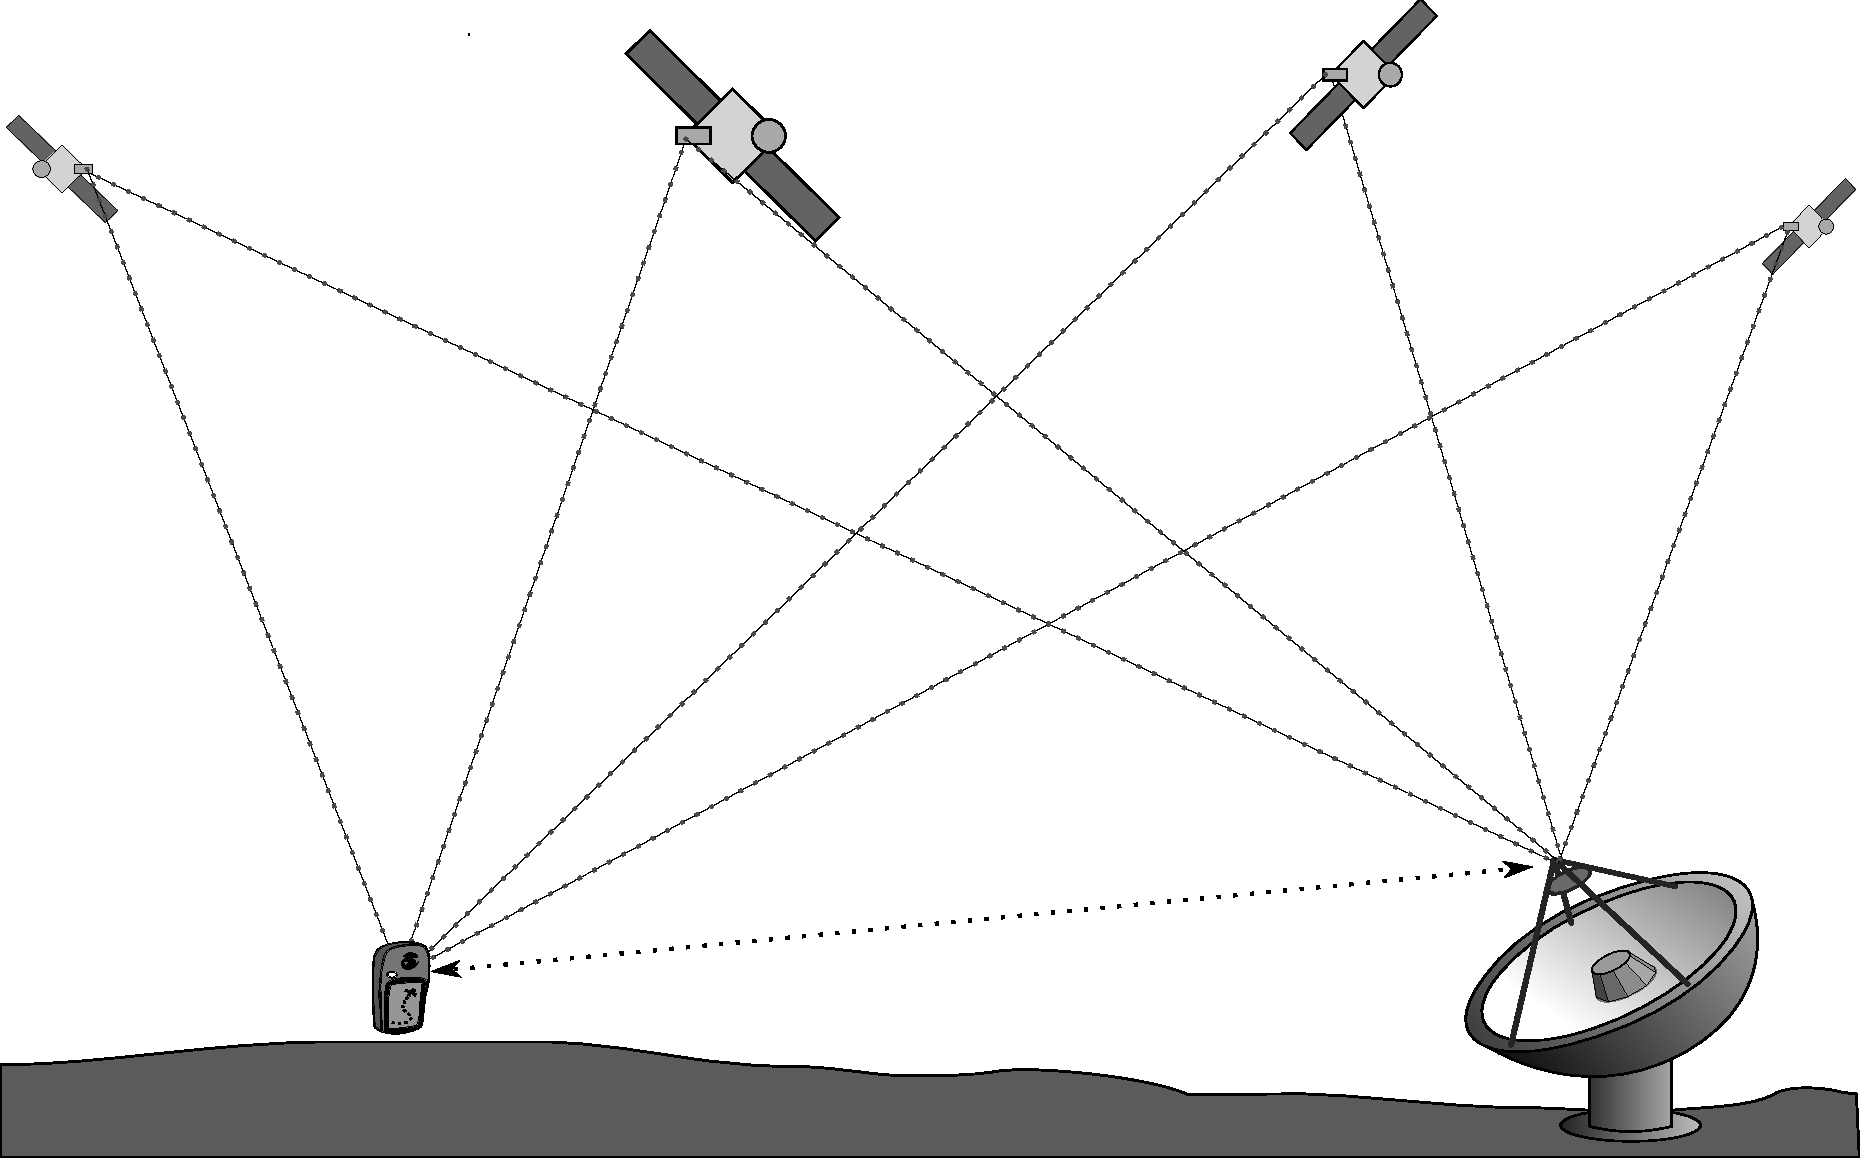
\includegraphics[width=.5\textwidth]{Fuentes_datos/DGPS.pdf}
\caption{\small Esquema de funcionamiento del GPS diferencial}
\label{Fig:DGPS} 
\end{figure}

Adem�s de la literatura abundante sobre GPS, los fabricantes de receptores GPS, muy populares hoy en d�a para numerosas actividades, ponen a disposici�n del p�blico una gran cantidad de informaci�n sobre sus productos y tambi�n sobre los fundamentos del sistema GPS. En ese sentido, una buena referencia es el sitio Web \cite{webTrimble}, donde puede encontrarse una descripci�n detallada de los distintos elementos del sistema GPS, acompa�ada de im�genes y animaciones sumamente did�cticas. En \cite{webHowWorkGPS} tambi�n puede encontrarse informaci�n de inter�s y f�cil acceso.


\subsection{Tipos de receptores}

La precisi�n del sistema global GPS depende del tipo de receptor GPS (o, en el lenguaje com�n, GPS a secas) que se emplee, obteni�ndose mayores precisiones con receptores m�s avanzados, siempre dentro de las posibilidades del propio sistema GPS.

En funci�n de sus caracter�sticas y de la forma en que operan, podemos distinguir los siguientes tipos de receptores GPS:

\begin{itemize}
	\item Receptores secuenciales. Establece conexiones secuenciales con los distintos sat�lites disponibles, estando conectado a uno o dos a lo sumo simult�neamente. Estos receptores son m�s econ�micos, ya que esta forma de operar requiere equipos menos complejos, aunque la precisi�n que se obtiene tambi�n es menor.
	\item Receptores continuos. Disponen de m�s canales de radio que los anteriores y ello permite que la conexi�n a los sat�lites sea continua, sin tener que alternar entre uno y otro. La precisi�n que se obtiene es mayor, pero se trata de equipos m�s caros.
	\item Receptores con canales multiplexados. El esquema de funcionamiento es similar al secuencial, alternando entre los distintos sat�lites y utilizando un �nico canal. No obstante, utilizan software m�s complejo y procesadores m�s potentes, de forma que esta alternancia se puede producir con una frecuencia mucho m�s elevada. 
\end{itemize}

\index{GPS!receptores}

A d�a de hoy, es habitual que incluso los GPS de menor coste tengan m�ltiples canales, permitiendo la conexi�n continua con un n�mero elevado de sat�lites.

Como hemos visto, las se�ales emitidas por los sat�lites contienen dos c�digos (C/A y P) que se transmiten modulados sobre dos ondas portadoras distintas (L1 y L2). No todos los receptores GPS son capaces de utilizar estos elementos de las se�ales, y en funci�n de ello podemos tambi�n clasificarlos. 

Los m�s sencillos �nicamente basan sus c�lculos en el c�digo C/A, mientras que los m�s avanzados y complejos son capaces de utilizar el c�digo P (encriptado, por lo que es necesaria una clave correspondiente), as� como las portadoras para un c�lculo m�s preciso, seg�n se explic� en un punto anterior.

Por �ltimo, y teniendo en cuenta que el sistema GPS mide las coordenadas $(x,y,z)$ y el tiempo, y que existen diferentes precisiones en funci�n de la tecnolog�a que los receptores utilicen, encontramos una gran variedad de unidades receptoras, seg�n estas se adapten para uno u otro uso principal. En l�neas muy generales, los siguientes son algunos de los tipos principales en funci�n de dicho uso.

\begin{itemize}
	\item GPS para uso general. Unidades peque�as y port�tiles, de bajo coste, para actividades al aire libre, donde no se requiere una precisi�n elevada sino simplemente un conocimiento de la posici�n aproximada. Se emplean, por ejemplo, para recoger rutas en senderismo o navegaci�n. Estas unidades, adem�s de informar de la posici�n y ser capaces de almacenar esta, suelen disponer de capacidades de representaci�n de mapas en pantalla, de forma que la informaci�n sobre la posici�n sea m�s �til para el usuario. Otros, como los navegadores GPS para coche, son capaces de calcular rutas �ptimas, combinando la posici�n calculada con una cartograf�a de v�as previamente incorporada al dispositivo.
		La figura \ref{Fig:gps_1}a muestra un receptor GPS de uso general.
	\item GPS para la medici�n topogr�fica. Unidades de medio tama�o, generalmente con una antena independiente que se conecta a la unidad y que el propio operario carga a la espalda. La antena garantiza mayor precisi�n y una mejor localizaci�n de sat�lites en condiciones tales como zonas bajo arbolado. Est�n pensados para un uso profesional en levantamientos o replanteos, ofreciendo buena precisi�n en todas las coordenadas. 
	En la figura \ref{Fig:gps_1}b puede verse unos de estos receptores.
	Estos son los GPS de mayor inter�s para el uso dentro de un SIG, ya que ofrecen datos de campo precisos que cumplen con las necesidades que habitualmente se tienen en un proyecto SIG. Los datos recogidos por estas unidades pueden ser sencillamente incorporados a un ordenador, y en ocasiones la propia unidad dispone de aplicaciones propias, m�s all� de la mera visualizaci�n de cartograf�a asociada, como en el caso anterior.
	\item GPS para la medici�n del tiempo. Estos GPS no resultan de tanto inter�s para su uso en un SIG, ya que se encuentran fijos en un punto y no conceden importancia a la localizaci�n espacial, sino tan solo al tiempo. Se utilizan en estudios que requieran una medici�n muy precisa del tiempo, ya que la referencia temporal que ofrece el sistema GPS es muy precisa y estable.
\end{itemize}

\begin{figure}
\centering
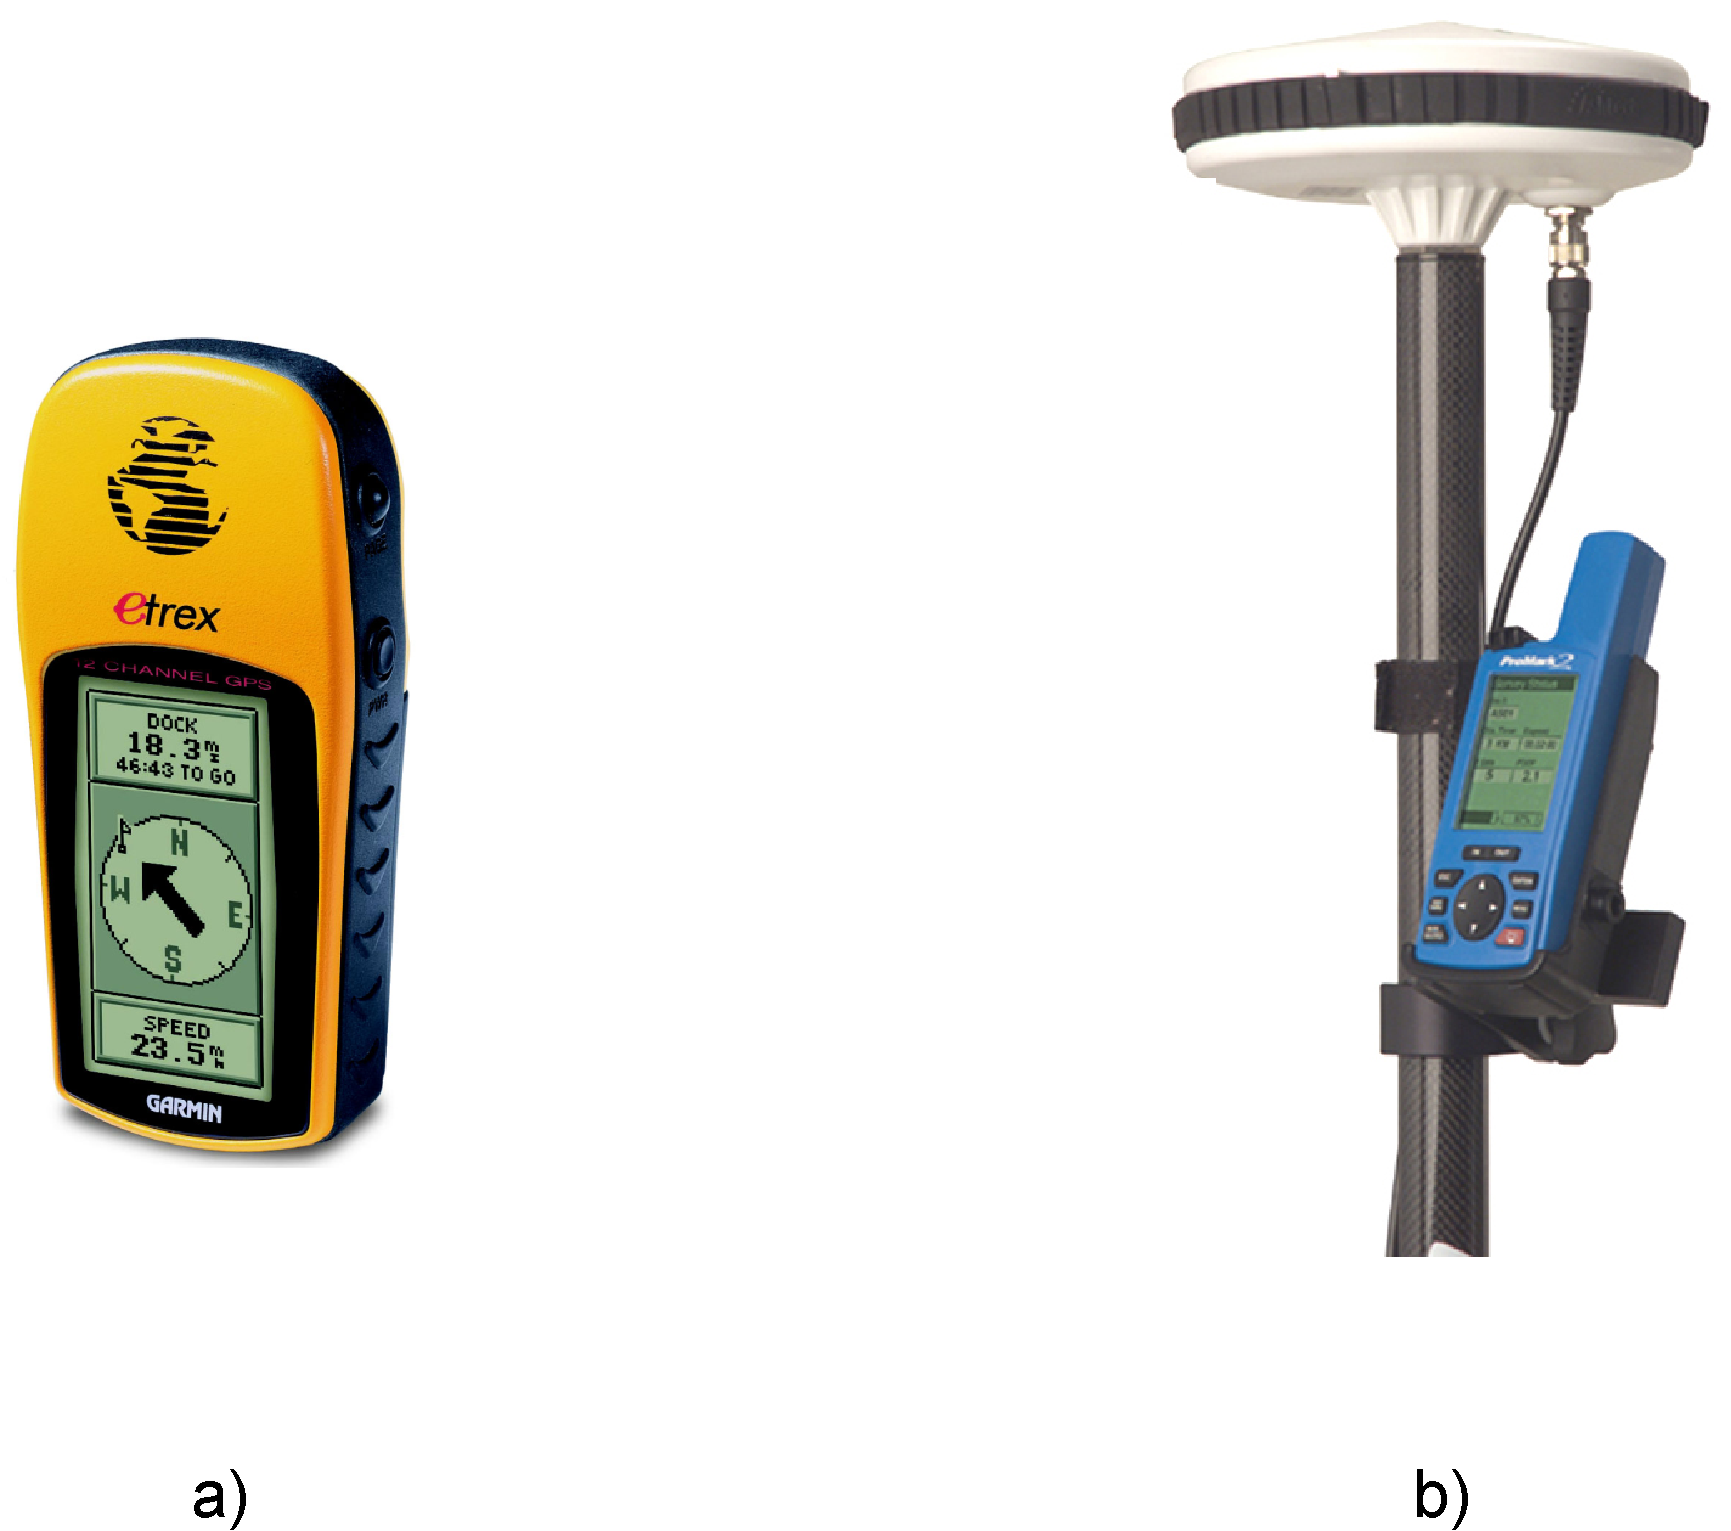
\includegraphics[width=.6\mycolumnwidth]{Fuentes_datos/gps.pdf}
\caption{\small Receptor GPS de bajo coste para uso general (a) y receptor GPS de alta precisi�n con antena externa (b)}
\label{Fig:gps_1} 
\end{figure}

%\begin{figure}
%\centering
%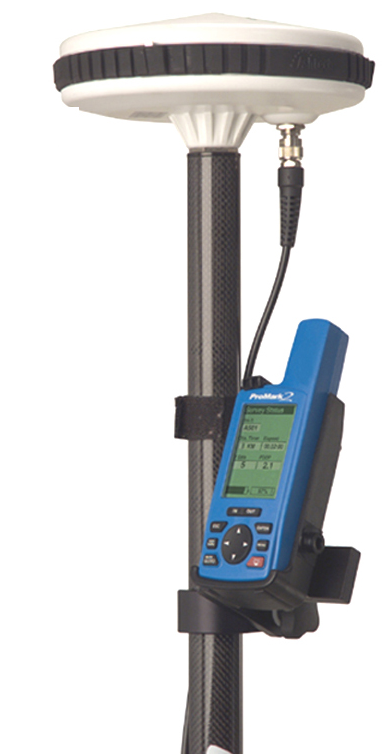
\includegraphics[width=.3\mycolumnwidth]{Fuentes_datos/gps_2.png}
%\caption{\small Receptor GPS de alta precisi�n con antena externa.}
%\label{Fig:gps_2} 
%\end{figure}

\subsection{Operaciones con la unidad GPS}

La forma en que utilizamos el receptor GPS para recoger los datos que emplearemos posteriormente en el SIG puede ser muy variada en funci�n del tipo de dato, la precisi�n necesaria o las caracter�sticas del propio receptor. 

Los receptores de menor coste est�n generalmente pensados para ser de utilidad directamente en el campo, por ejemplo para localizar un punto concreto y conocer la direcci�n en la que hay que moverse para llegar hasta �l, pero tienen tambi�n capacidad para recoger coordenadas. Estas capacidades son las que resultan de inter�s desde el punto de vista de un SIG, ya que las coordenadas recogidas ser�n despu�s los datos que llevemos a este.

Por su parte, las unidades de mayor precisi�n est�n concebidas para tareas tales como levantamientos topogr�ficos, donde la toma de datos es lo fundamental, pero tambi�n para otras tales como replanteos, donde se requiere situar un punto de coordenadas conocidas. Al igual que en el anterior, las actividades que pueden llevarse a cabo con estos GPS y que interesan desde el punto de vista del SIG son aquellas que van a recoger coordenadas, pues son las que generan datos y convierten al GPS en una fuente de ellos.

Las capacidades de recogida de datos en una unidad GPS de bajo coste permiten almacenar puntos o trazados completos, encontr�ndose el operario inm�vil o bien en movimiento a lo largo de dicho trazado. Es habitual utilizar los vocablos ingleses de la terminolog�a GPS para denotar los distintos elementos que pueden recogerse, conoci�ndose a un punto de inter�s aislado como \emph{waypoint} y un trazado como \emph{track}. Una serie ordenada de \emph{waypoints} se conoce como \extr{route} (ruta).\index{Waypoint}\index{Track}\index{Route}

En el trabajo con el receptor GPS, el operario se puede detener en un punto cualquiera y memorizar las coordenadas del mismo, a�adiendo as� un \emph{waypoint} a la lista de los ya almacenados. Para crear un trazado, se suele disponer de funcionalidades de recogida autom�tica de puntos, de tal modo que el receptor memoriza estos a intervalos fijos de tiempo. El operario simplemente ha de desplazarse por el trazado y dejar que el receptor haga su trabajo mientras tanto. Dependiendo del tipo de dato que quiera obtenerse, la edici�n posterior en gabinete habr� de ser m�s o menos intensa. 

Esta edici�n no est� relacionada solo con la introducci�n de correcciones, sino con la interpretaci�n de los distintos puntos recogidos. Por ejemplo, para registrar el trazado de una calle, el operario puede recorrerla, pero es probable que no lo haga de forma perfectamente rectil�nea. El trabajo posterior con el conjunto de puntos debe resultar en la obtenci�n de una l�nea recta a partir de estos, y ello requiere la interpretaci�n de los datos disponibles.

Pese a que la precisi�n de estas unidades es limitada y no permiten t�cnicas avanzadas de correcci�n (tal precisi�n no es necesarias para las actividades tales como senderismo o navegaci�n para las que han sido dise�ados estos receptores), los GPS de uso cotidiano pueden ser una fuente de datos de primer orden para la recogida de datos. Un ejemplo significativo de ello es el proyecto OpenStreetMap\cite{webOSM}, un proyecto colaborativo para crear mapas libres  cuya principal fuente de datos son unidades GPS sencillas.\index{OpenStreetMap} Este proyecto es uno de los muchos que existen actualmente de este tipo, los cuales se engloban dentro de la idea de \emph{Informaci�n Geogr�fica Voluntaria o Participativa}, sobre la que hablaremos algo m�s adelante en el apartado \ref{VGI}.

Para trabajos de mayor precisi�n tales como levantamientos topogr�ficos, estos receptores no son, sin embargo, suficientes. El uso de receptores m�s precisos y de t�cnicas avanzadas es necesario para obtener precisiones mayores, que pueden ser incluso milim�tricas. 

Estos receptores pueden emplearse individualmente del mismo modo que se hace con un GPS de bajo coste, y registrar puntos de forma similar. La verdadera potencia, no obstante, se obtiene cuando se realizan mediciones con la ayuda de una o varias unidades adicionales, las cuales aportan valores de referencia que permiten aumentar la precisi�n. 

Entre el receptor m�vil y el de referencia se establece una \emph{l�nea base}, y en el c�lculo de la posici�n lo que se calcula es el vector $(x, y, z)$ que une a ambas. Se trata pues, de una medici�n relativa, ya que expresa la posici�n del receptor m�vil a partir de la del receptor de referencia. Puesto que la posici�n de este �ltimo se conoce con gran precisi�n y ese vector tambi�n se calcula con precisi�n, la posici�n buscada que se obtiene es altamente precisa.

La principal ventaja con respecto a m�todos topogr�ficos cl�sicos es que no es necesario que haya visibilidad entre los dos receptores. De esta forma, puede utilizarse una estaci�n de referencia aunque no sea visible desde un punto cuyas coordenadas queremos medir, y las l�neas base pueden ser de mayor longitud.

Otras ventajas tambi�n destacables son el hecho de que puede obtenerse una productividad mucho mayor, ya que una �nica unidad de referencia puede ser utilizada por varias unidades m�viles.

El n�mero de t�cnicas existentes en la actualidad para realizar este tipo de mediciones (ya sea con uno o con varios receptores) es variada. El hecho de que se busquen mediciones precisas hace que se realicen mediciones utilizando la fase de la portadora, que como vimos implica una mayor necesidad de tiempo para registrar correctamente una posici�n. En funci�n de las caracter�sticas de la linea base y los requerimientos concretos del trabajo, ser�n unas u otras las m�s adecuadas para cada caso. 

La diferencia principal entre estas t�cnicas es el tiempo necesario para la recogida de un punto. En general, un mayor tiempo equivale a una mayor precisi�n. Entre las t�cnicas habituales, cabe citar las siguientes:

\begin{itemize}
	\item Est�tico. En base a dos puntos de referencia (con una unidad GPS fija en cada uno de ellos), se calcula la posici�n de un tercero en un punto dado. Se trata del m�todo m�s preciso, pero requiere tiempos de observaci�n muy largos (superiores a una hora), lo que lo hace inadecuado para levantamientos o replanteos. Este tipo de procedimientos se emplean casi exclusivamente en trabajos geod�sicos y las lineas base pueden ser de gran longitud. 
	\item Est�tico r�pido. Igual que el anterior, pero con tiempos menores, del orden de 5--10 minutos por punto medido.	
	\item Cinem�tico. En el m�todo cinem�tico los tiempos son a�n menores que en el est�tico r�pido, del orden del minuto. El fundamento de la t�cnica es distinto a los anteriores, ya que tras la inicializaci�n el receptor m�vil puede desplazarse con m�s velocidad y no es necesario que se detenga durante un periodo largo de tiempo en cada punto, pero ello exige que durante el desplazamiento tanto la unidad m�vil como la fija de referencia mantengan la recepci�n de las se�ales, que han de ser de al menos cuatro sat�lites (preferiblemente cinco), y los mismos para ambas unidades. Si alguna de ellas pierde la conexi�n, se hace necesario repetir de nuevo el proceso de inicializaci�n \cite{Remondi1988IN}.
	
	Existe una gran variedad de procedimientos de tipo cinem�tico, cuya filosof�a es esencialmente la misma, pero bajo nombres distintos. Aunque pueden existir diferencias en los fundamentos te�ricos, la forma de proceder es en muchos casos muy similar. T�cnicas como \emph{Stop \& Go}\index{Stop \& Go} o \emph{pseudocinem�tico} pueden incluirse en este tipo de m�todos. En general, estos y otros se engloban bajo la denominaci�n de procedimientos cinem�ticos, aunque sus caracter�sticas sean distintas en cada caso. 
	
	Muchos de estos procedimientos vienen definidos por el equipo a utilizar, y los tiempos de paradas en cada punto medido, as� como otros aspectos, son recomendados por el propio fabricante. La forma m�s correcta de llevar a cabo una toma de datos en campo, en este caso, es seguir las indicaciones concretas del fabricante de para cada producto.
	
	Un caso particular dentro de los m�todos cinem�ticos es el \emph{cinem�tico en tiempo real} (RTK)\footnote{Real Time Kinematic}, en el que, a diferencia de los anteriores, las correcciones necesarias se efect�an en tiempo real y no requieren postproceso. Se trata de la t�cnica m�s actual, y proporciona al operario mediciones exactas de su posici�n de forma instant�nea, con las ventajas que ello conlleva. Las mediciones son m�s precisas, ya que el operario que las toma conoce el valor recogido en el mismo momento de hacer la medici�n, y puede de esa forma realizar una comprobaci�n en el acto. Informaci�n m�s detallada sobre esta t�cnica puede encontrarse en \cite{Rizos1998BCG}.
\end{itemize}\index{Real Time Kinematic}

Para profundizar m�s al respecto, en \cite{Asenjo1997UPV} puede encontrarse informaci�n sobre la realizaci�n de levantamientos con GPS, as� como en \cite{GPSUSArmy}.

En base a los ejemplos anteriores, y para concluir esta parte, podemos dar una clasificaci�n de las operaciones con un receptor GPS en funci�n de tres criterios b�sicos: el n�mero de unidades que se emplean simult�neamente, el movimiento (o ausencia de �l) del receptor y el momento en el que se obtiene el dato ya listo para su utilizaci�n posterior.

Seg�n el n�mero de unidades, tenemos:

\begin{itemize}
	\item Absolutas. Se tiene un �nico receptor y un �nico operario. La posici�n se calcula con la informaci�n de los sat�lites, sin apoyo de otra unidad adicional.
	\item Relativas. Se emplea una unidad adicional a modo de referencia. Las medidas se basan en la informaci�n de los sat�lites y la que aporta dicha unidad de referencia, y la posici�n se calcula en relaci�n a esta en lugar de en t�rminos absolutos. Estas operaciones alcanzan un grado de precisi�n mayor que las de tipo absoluto.
\end{itemize}

Atendiendo al movimiento del receptor encontramos:

\begin{itemize}
	\item Est�ticas.
	\item Cinem�ticas.
	\item Variantes intermedias.
\end{itemize}

Por �ltimo, en funci�n de la obtenci�n de datos, distinguimos:

\begin{itemize}
	\item En tiempo real. Las correcciones pertinentes se realizan en el acto, y el resultado que se visualiza en el receptor o se almacena en este ya ha sido filtrado y corregido.
	\item Con necesidad de postproceso. Las correcciones se realizan en gabinete posteriormente, con informaci�n que el receptor no posee o no es capaz de procesar de modo inmediato durante su utilizaci�n.
\end{itemize}

\subsection{Integraci�n de GPS y SIG}

\index{GPS!integraci�n con SIG}

La utilidad de un GPS como fuente de datos para el trabajo en un SIG es innegable. Multitud de trabajos que requieren la toma de datos en campo y la medici�n de coordenadas pueden efectuarse ventajosamente con equipos GPS, y la informaci�n derivada de ese uso puede ser posteriormente incorporada a un SIG.

EL GPS puede emplearse como una fuente de datos est�tica (se utiliza como herramienta para la creaci�n de una capa de informaci�n geogr�fica y esta despu�s se emplea en el SIG de la forma habitual), o bien para la obtenci�n de datos en tiempo real. Los SIG sobre dispositivos m�viles (v�ase el apartado \ref{SIG_Moviles}) pueden aprovechar los receptores GPS que estos dispositivos habitualmente incorporan, y alimentarse con los datos de dichos receptores en tiempo real.

Un caso particular de esto son los cada d�a m�s populares navegadores GPS. Estos dispositivos aunan el receptor GPS y una aplicaci�n de tipo SIG que presenta un visor y permite ejecutar un n�mero reducido de procesos, en concreto los de c�lculo de rutas �ptimas entre dos puntos a trav�s de una red de comunicaci�n (apartado \ref{Rutas_optimas}). Uno de los puntos (el de destino) es fijado por el usuario, mientras que el punto de origen es el punto actual en que se encuentra el dispositivo, que se obtiene a partir del GPS.

Como herramientas est�ticas, el trabajo en campo con un GPS genera un conjunto de puntos o de trazados, que pueden f�cilmente transferirse al ordenador para poder trabajar con ellos. Este trabajo puede realizarse dentro de un SIG, ya que, o bien este incluye la capacidad de importar los archivos generados por el GPS, o el software que acompa�a a dicho GPS incorpora herramientas para ayudar en la comunicaci�n entre SIG y GPS.

Adem�s de la informaci�n posicional que deriva del sistema GPS, los receptores GPS pueden incorporar elementos que permitan la entrada de la componente tem�tica asociada a las distintas entidades, es decir, los atributos. Si solo se registra la componente espacial, la informaci�n que se almacena en el GPS es de mucha menos utilidad que si se acompa�a de atributos.

Las funcionalidades incorporadas en el receptor suelen ser sencillas, pero permiten que desde este se pueda llevar a cabo todo el proceso de creaci�n de la capa que posteriormente se emplear� en el SIG. El trabajo de campo incluye de este modo tanto el registro y creaci�n de las entidades como la edici�n de las propiedades no espaciales de estos. Existe, no obstante, la posibilidad de completar la fase de introducci�n de atributos en el SIG, durante el trabajo en gabinete, lo cual en ocasiones resulta m�s sencillo y pr�ctico.

El volumen de trabajo que se requiere una vez que los datos han sido recogidos depender� tambi�n de las necesidades de precisi�n que se presenten y del tipo de trabajo en que se enmarque dicha recogida de datos. La realizaci�n de correcciones y la edici�n avanzada de los datos no puede en ocasiones realizarse dentro de un SIG, ya que este no dispone de las herramientas necesarias para un tratamiento avanzado de los datos del GPS. El SIG est� preparado para trabajar con las coordenadas que salen del GPS, pero este puede almacenar m�s datos (datos <<en bruto>>), que pueden procesarse en gabinete para la obtenci�n de dichas coordenadas de forma m�s precisa. Para realizar esta tarea  es necesario software especializado, y las funcionalidades del SIG se emplear�n posteriormente, cuando ya se hayan verificado los datos del GPS y elaborado las capas correspondientes.

Para el lector interesado, una referencia completa sobre el uso de GPS de cara a la integraci�n de los datos en un SIG es \cite{Steede2000ESRI}.  En el ya mencionado apartado \ref{SIG_Moviles} veremos con detalle la tecnolog�a de los SIG m�viles, un �mbito en el que SIG y GPS se unen para conformar herramientas conjuntas. 

\section{Informaci�n Geogr�fica Voluntaria}\label{VGI}

Hemos mencionado ya que los dispositivos tales como receptores GPS de bajo coste pueden emplearse para recoger informaci�n geogr�fica y crear datos geogr�ficos, y que cuando esto se une a los conceptos participativos de la denominada Web 2.0, surgen iniciativas de gran inter�s en las que el usuario de a pie, sin necesidad de una formaci�n espec�fica como cart�grafo, puede aportar sus datos para que otros los exploten posteriormente. Aunque no se trata de una fuente de datos como tal, y los elementos y dispositivos empleados ya los hemos visto a lo largo de este cap�tulo, el cambio que supone la inclusi�n de una filosof�a acorde con las ideas de la Web 2.0 es tan notable que merece ser tratado por separado. No se trata de un cambio en la propia toma o preparaci�n de datos, o de una tecnolog�a nueva que se aplique a estos, sino de un cambio social y filos�fico que redefine el propio concepto de la informaci�n geogr�fica en lo que a la creaci�n del dato geogr�fico respecta, y cuyas consecuencias son ciertamente importantes, ya que abren el �mbito de la creaci�n cartogr�fica a un nuevo y amplio grupo de personas.\index{Web 2.0}

Se conoce como \emph{Informaci�n Geogr�fica Voluntaria o Participativa} (en ingl�s Volunteered Geographical Information, VGI)\cite{Goodchild2007VGI} al uso de Internet para crear, gestionar y difundir informaci�n geogr�fica aportada voluntariamente por usuarios de la propia red. El conjunto de herramientas y t�cnicas que emplean esos usuarios para aportar su informaci�n conforma lo que se ha dado en llamar \emph{neogeograf�a}. La comparaci�n entre proyectos de creaci�n de VGI y la bien conocida Wikipedia, tal y como se coment� en otro punto anterior en este mismo cap�tulo, sirve perfectamente para ilustrar qu� es lo que entendemos por VGI y neogeograf�a.
\index{Neogeograf�a}\index{VGI}\index{Informaci�n Geogr�fica Voluntaria|see{VGI}}\index{Wikipedia}

En el caso particular de esta �ltima, la neogeograf�a ha supuesto un profundo cambio en algunas de las ideas b�sicas de la cartograf�a, modificando asimismo la concepci�n tradicional de la informaci�n geogr�fica, sus caracter�sticas o el papel que esta ven�a desempe�ando en muchos �mbitos (o incluso d�ndole un papel en campos donde con anterioridad el uso de informaci�n geogr�fica era escaso). Algunas de las ideas principales sobre la neogeograf�a son las siguientes:

\begin{itemize}
	\item Popularizaci�n y democratizaci�n. La producci�n cartogr�fica ha estado siempre en manos de gobiernos u organismos, y en muchas ocasiones fuertemente censurada debido a su elevado valor estrat�gico. Con la VGI, la creaci�n de informaci�n geogr�fica se democratiza y se convierte en un proceso participativo libre y sin restricciones.  Se invierte el esquema <<hacia abajo>> de producci�n y uso de informaci�n geogr�fica.
	\item Los ciudadanos se convierten en <<sensores>> y tienen mayor consciencia de su realidad geo--espacial.
	\item Se elimina parte del <<misticismo>> de la producci�n de informaci�n geogr�fica	
\end{itemize}

En parte, estas ideas son tambi�n comunes a otros fen�menos basados en la Web 2.0, ya que todas se fundamentan en una mayor democratizaci�n de la informaci�n, sea esta geogr�fica o no. Tambi�n se comparten algunos de los problemas o cr�ticas que otros �mbitos han recibido al adoptar esquemas de producci�n similares. Por ejemplo, la calidad de la informaci�n es puesta en entredicho al promover la participaci�n de todo tipo de personas, con independencia de su perfil. En el caso de la informaci�n geogr�fica, con una producci�n tradicionalmente como hemos dicho limitada a profesionales muy especializados, esto es especialmente relevante. Con la proliferaci�n de la VGI, se da voz y poder sobre la informaci�n geogr�fica a individuos en gran medida sin formaci�n, que no obtienen un beneficio tangible obvio y no pueden aportar garant�as de veracidad o autoridad alguna. Esto puede plantear dudas l�gicas acerca de la conveniencia de usar esa informaci�n.

No debe olvidarse no obstante, que la Web 2.0 tambi�n tiene sus mecanismos de regulaci�n, y que en otros casos ya se ha demostrado que, para otros tipos de informaci�n, la calidad y rigor de esta no es inferior a la creada con esquemas m�s cl�sicos y menos abiertos. Un hecho particularmente curioso que tiene lugar a este respecto con la informaci�n geogr�fica es el relacionado con los denominados \emph{elementos trampa}, y particularmente con el m�s popular de ellos, las \emph{calles trampa}. Aunque se trata de una pr�ctica negada por buena parte de los productores de cartograf�a, es sabido que estos introducen elementos err�neos (tales como una calle inexistente en un callejero) como medida para proteger sus derechos de autor y poder reconocer copias ilegales. En el caso de la VGI, puesto que no existe esa necesidad ya que la informaci�n generada y aportada por los voluntarios es libre, no existen este tipo de errores intencionados. La comparaci�n de informaci�n geogr�fica cl�sica con VGI ha puesto de manifiesto que se trata de una pr�ctica real que, obviamente, disminuye la calidad del dato geogr�fico.

Por otra parte, el hecho de que se use equipo de bajo coste y los usuarios no sean t�cnicos especializados no es necesariamente un problema. Un usuario sin formaci�n no est� capacitado para efectuar un levantamiento topogr�fico preciso, pero s� para situarse delante de la puerta de una tienda y marcar su posici�n, a�adiendo esta a un proyecto que catalogue los comercios de la zona y su localizaci�n. Este tipo de informaci�n geogr�fica, de puntos de inter�s muchas veces no recogidos en cartograf�a m�s especializada, constituye una gran parte de la VGI, y las metodolog�as e instrumental con que se crea son m�s que suficientes para otorgarle validez y precisi�n adecuada al uso del que posteriormente va a ser objeto.

En resumen, la neogeograf�a es en la actualidad un fen�meno que no debe dejarse de lado, ya que los proyectos que aglutina se est�n convirtiendo paulatinamente en proveedores fundamentales de datos cuya calidad en muchos casos es excelente.

Aunque las hemos tratado dentro de este cap�tulo dedicado a las fuentes de datos, la VGI y la neogeograf�a tienen una indudable vinculaci�n con todo lo desarrollado en la parte de este libro dedicada al factor organizativo, ya que se trata de un fen�meno social m�s que t�cnico. De igual modo, el cap�tulo \ref{Otros_tecnologia}, dedicado a los SIG m�viles, est� tambi�n muy relacionado con ambas, puesto que son los dispositivos y aplicaciones que veremos entonces, as� como los servicios sobre ellos, los que han posibilitado el desarrollo de la neogeograf�a y la abundante producci�n actual de VGI. \index{SIG m�vil}


\section{Sobre cartograf�a de elevaciones}

La cartograf�a de elevaciones es probablemente la de mayor importancia de entre todas las que se emplean de forma habitual dentro de cualquier proyecto SIG. Su relevancia deriva del hecho fundamental de que la practica totalidad de procesos que se estudian en un SIG tienen alg�n tipo de componente relacionada con el terreno y su relieve, y por tanto puede obtenerse amplia informaci�n sobre dichos procesos a partir de una capa con datos de elevaci�n.

Como dato relevante, dedicaremos en este libro un cap�tulo entero, el \ref{Geomorfometria}, al conjunto de operaciones de an�lisis basadas en el MDE\index{Modelo Digital de Elevaciones}, que van desde el simple c�lculo de pendientes hasta la extracci�n de par�metros m�s complejos, pasando por la definici�n del comportamiento hidrol�gico de una zona seg�n las caracter�sticas de su relieve, entre otros. Asimismo, gran n�mero de otras formulaciones que veremos en la parte dedicada a procesos tienen su principal aplicaci�n sobre datos de elevaci�n, en particular los m�todos de interpolaci�n que veremos en el cap�tulo \ref{Creacion_capas_raster}, y que nos permitir�n crear cartograf�a de elevaciones en formato r�ster. Este es, como veremos, el formato preferido para el an�lisis de la cartograf�a de elevaciones, ya que ofrece un mayor abanico de posibilidades frente a otros.\index{Interpolaci�n}

Aunque el formato r�ster es el m�s indicado para llevar a cabo los an�lisis correspondientes, la cartograf�a de elevaciones puede crearse originalmente con muy diversas caracter�sticas. De igual modo, y debido tambi�n a la gran importancia de este tipo de capas, su origen puede ser muy variado, ya que son muchas las t�cnicas distintas que existen para su creaci�n. Es de inter�s, por tanto, exponer en este cap�tulo sobre fuentes de datos algunas de las ideas principales relativas a la creaci�n de capas de elevaciones, las caracter�sticas de estas o las ideas fundamentales que residen tras las metodolog�as m�s importantes. Posteriormente, esto nos ayudar� a entender mejor las restantes formulaciones y conceptos relativos al manejo y an�lisis de este tipo de cartograf�a, abundantes en este libro como ya se ha dicho.

A modo de resumen, he aqu� una lista de metodolog�as a partir de las cuales puede obtenerse cartograf�a de elevaciones, gran parte de las cuales han sido tratadas con detalle antes en este mismo cap�tulo.

\begin{itemize}
\item GPS. Como ya sabemos, un GPS toma datos no solo de la posici�n que ocupa en coordenadas $x$ e $y$, sino tambi�n su elevaci�n. La utilizaci�n de GPS permite obtener una nube de puntos de elevaci�n, aunque si esta ha de cubrir un territorio amplio y con cierta precisi�n en las medidas, resulta poco id�neo el trabajar con esta tecnolog�a, ya que es costoso en tiempo. Es m�s adecuada para obtener levantamientos precisos de �reas m�s reducidas, donde se demuestra como una herramienta sumamente eficaz.
\item Digitalizaci�n de curvas de nivel. En ocasiones la cartograf�a de elevaciones ya existe, aunque no en el formato adecuado para su empleo en un SIG. Ya conocemos los m�todos de digitalizaci�n de entidades, tanto manuales como autom�ticos, y ya sea en pantalla o en equipo especializado, y mediante ellos podemos digitalizar las curvas de nivel, obteniendo una capa de l�neas con la informaci�n altitudinal que contiene un mapa topogr�fico habitual.\index{Digitalizaci�n!de curvas de nivel}\index{Curva!de nivel!digitalizaci�n}
\item Estereograf�a. A partir de pares estereosc�picos, y con el concurso de una estaci�n fotogram�trica digital pueden delinearse l�neas o puntos de una elevaci�n dada, digitalizando as� la informaci�n altim�trica. El procedimiento es similar a la simple digitalizaci�n de curvas de nivel, solo que en este caso estas no est�n presentes expl�citamente en las im�genes de partida, y se infieren a partir de la visualizaci�n tridimensional de las mismas.\index{Estereograf�a}
\item Interferometr�a. La interferometr�a es una t�cnica cuyos fundamentos son en cierta medida similares a los de la estereograf�a, pues se basan en la informaci�n recogida de un punto concreto desde dos puntos distintos. Si en el caso de emplear simples im�genes esto permit�a crear una imagen tridimensional, en el caso de la interferometr�a el estudio de las diferencias de fases entre las ondas recibidas en dos puntos distintos permite el c�lculo de distancias. Se trata, por tanto, de un proceso automatizado, que requiere menos intervenci�n que en el caso de la restituci�n fotogram�trica.\index{Interferometr�a}

Un uso muy habitual de esta t�cnica es con los denominados \emph{Radares de Apertura Sint�tica}\footnote{Synthetic Aperture Radar (SAR)}, utilizado por ejemplo en el caso de la misi�n SRTM, que rese�amos anteriormente como producto importante. La medici�n desde dos puntos puede hacerse con dos pasadas de sat�lite (caso por ejemplo del ERS) o bien en una sola si la plataforma dispone de dos receptores separados una cierta distancia (caso del SRTM). En \cite{SARInterferometry} puede encontrarse una descripci�n detallada de este tipo de t�cnicas y las etapas que comprenden.
\item LiDAR. La t�cnica m�s avanzada en la actualidad es el uso de aparatos de altimetr�a basados en l�ser, como el LiDAR, que ya hemos visto en este mismo cap�tulo. El LiDAR ofrece posibilidades muy interesantes tales como la obtenci�n de MDE y MDS (Modelo Digital de Superficie) por separado. \index{Radar de Apertura Sint�tica}\index{Synthetic Aperture Radar}\index{LiDAR}\index{SRTM}\index{Modelo Digital de Superficie}

El resultado de un trabajo con LiDAR es una nube de puntos, normalmente en un n�mero muy elevado debido a la precisi�n del instrumento, la cual puede emplearse para crear otro tipo de capas, tales como capas r�ster. El nivel de postproceso que se requiere para la obtenci�n final de una capa es mucho menor que con otras t�cnicas.
\end{itemize}

A la hora de plantear un proyecto SIG, debe elegirse entre estas fuentes, tanto si se desea adquirir la cartograf�a ya elaborada como si se desea crearla a partir de otras fuentes. La variedad de opciones existentes es grande, y cada una de ellas tiene sus caracter�sticas peculiares. Para saber m�s al respecto, algunas referencias donde puede encontrarse una comparaci�n entre las metodolog�as anteriores son \cite{Nikolakopoulos2006IJRS}, \cite{Mercer1999ISPRS} y \cite{Mercer2001PW}.

\section{Formatos de archivo}\label{Formatos_archivo}

Como hemos visto, las fuentes de datos son muy variadas, y a la hora de elaborar un proyecto SIG podemos recoger datos de muchas procedencias distintas. Conocer todas estas fuentes de datos es importante para elaborar una base de datos geogr�fica que permita obtener los mejores resultados posibles, pero tambi�n lo es el conocer la forma en que esos datos pueden obtenerse. Los datos geogr�ficos se van a almacenar en archivos, existiendo muchos formatos de archivo distintos para recoger un mismo conjunto de datos.

Estos archivos son la materializaci�n de los modelos de almacenamiento que ve�amos en el apartado \ref{Modelos_almacenamiento}, y su existencia obedece a distintas razones. Pueden haber sido definidos por alguna casa comercial para ser utilizados en su software, por un colectivo, o bien pueden ser est�ndares internacionales definidos para tratar de homogeneizar la forma en que se presentan los datos dentro de un determinado �mbito de trabajo.

Datos de una misma procedencia pueden presentarse de forma distinta si se emplean diferentes formatos de archivo. Las circunstancias por las cuales se opta por uno u otro formato pueden basarse �nicamente en el hecho de que el software empleado soporte o no dicho formato, pero deber�an fundamentarse en las propias caracter�sticas del formato y lo adecuadas que estas son para recoger la informaci�n con la que trabajamos.

La existencia de muchos formatos de archivo dificulta el trabajo con los datos en un SIG, principalmente porque ning�n SIG implementa la capacidad de poder <<leer>> todos los formatos existentes. La interoperabilidad y la comunicaci�n entre distintos SIG, o incluso entre un SIG y otras aplicaciones (bases de datos, aplicaciones para manejo de im�genes, aplicaciones CAD) no es completa, y el aprovechamiento de todos los datos disponibles dentro de un proyecto requiere normalmente tiempo para la gesti�n adecuada de datos en formatos variados.\index{CAD}

Un problema m�s serio, no obstante, es el desconocimiento por parte de los usuarios de las implicaciones que tiene el uso de uno u otro formato, ya que en ocasiones no permiten aprovechar de modo pleno los datos de que se dispone. Por ejemplo, dentro de un SIG es habitual emplear datos procedentes de CAD. Los datos en un CAD se almacenan en formatos de datos definidos por esas aplicaciones CAD, los cuales han sido definidos para satisfacer las necesidades del �mbito de trabajo en el que se han desarrollado (el dise�o asistido por ordenador). Aunque los SIG pueden leer esos formatos de archivo y se encuentra informaci�n muy valiosa almacenada en ellos, no son ideales para el manejo de capas de datos SIG (en este caso, capas vectoriales), y es importante conocer este hecho.

La existencia de librer�as que act�an a modo de interpretes facilita el desarrollo de aplicaciones SIG con capacidades de lectura y escritura en muchos formatos distintos, pero a�n as� se requiere un cierto grado de comprensi�n de estos por parte del usuario.

Debemos pensar asimismo que los formatos de archivo no solo se emplean en un proyecto SIG para los datos de entrada, sino tambi�n para almacenar los resultados que se generan a lo largo de ese proyecto. Estos datos ser�n utilizados en el propio SIG en otras ocasiones posteriores, o bien en otros programas. De este modo, tomamos datos que pueden provenir de aplicaciones y fuentes diversas, pero tambi�n <<damos>> datos a esas aplicaciones, por lo que la comunicaci�n es bidireccional. Puesto que es a trav�s de archivos como dicha comunicaci�n se produce, y estos tienen que tener un formato dado, el conocimiento de estos formatos mejora tanto esa comunicaci�n como la potencialidad de nuestros datos para todo tipo de uso, ya sea dentro o fuera de un SIG.

En esta secci�n no se pretende describir todos los formatos existentes, ya que estos son demasiados y ello no tendr�a sentido. Se describir�n solo los m�s populares (que no siempre han de ser necesariamente los mejores) para que el lector obtenga un conocimiento general de \emph{c�mo} se van a presentar sus datos, y a trav�s de estos formatos se describir�n los principales enfoques existentes, que son los que realmente ha de conocer un usuario de SIG para saber discernir si un formato es o no adecuado para sus datos y las operaciones que quiere aplicar sobre ellos.

Junto con estos formatos de archivo, en el cap�tulo \ref{Estandares} se presentan los est�ndares de datos, que tambi�n se emplean para el intercambio y almacenamiento de datos SIG, y que presentan una relaci�n estrecha con el contenido de esta secci�n. El capitulo \ref{Bases_datos}, que veremos dentro de esta misma parte, tambi�n guarda relaci�n con este apartado, pues estudia las diferentes formas en que los SIG han solucionado a lo largo del tiempo el acceso a los datos, incluyendo entre ellas el acceso directo a archivos.

\subsection{Formatos para datos r�ster}

Los formatos de archivo para datos r�ster son muy abundantes, existiendo numerosas alternativas con diferencias en ocasiones notables entre s�. Debido a que uno de los datos r�ster m�s habituales en un SIG son las im�genes, a los formatos de datos espec�ficos para datos r�ster hay que sumar aquellos ya existentes para el almacenamiento de im�genes, que son de por s� muy variados. Estos formatos, adaptados a la naturaleza particular de las im�genes de un SIG, pueden emplearse para almacenar datos r�ster y son de hecho de uso habitual en el �mbito de los Sistemas de Informaci�n Geogr�fica.

\subsubsection{Formatos para im�genes}

Como ya sabemos, las im�genes son un tipo de dato muy habitual en un SIG, y estas se corresponden con el modelo de datos r�ster. Por ello, los formatos de archivo empleados para el almacenamiento de im�genes digitales se emplean tambi�n para las im�genes particulares que utilizamos en un SIG (por ejemplo, fotograf�as a�reas o mapas escaneados, seg�n vimos antes en este mismo cap�tulo), e incluso para otros datos r�ster que no son im�genes como tales, como por ejemplo un Modelo Digital de Elevaciones.

Los formatos de archivo para im�genes son adecuados para recoger los colores de las im�genes, pero esto no es suficiente a la hora de almacenar otros valores (por ejemplo, valores decimales) o bien cuando son necesarios un n�mero m�s elevado de bandas, como en el caso de im�genes hiperespectrales. 

Una imagen en blanco y negro o en escala de grises contiene una banda. Una imagen en color contiene tres, ya que los colores se expresan como una terna de colores b�sicos: rojo, verde y azul. Este es el fundamento del modelo de color RGB, en el cual todo color es la combinaci�n de distintas intensidades de los anteriores colores b�sicos. Las intensidades de cada banda (o las intensidades de la �nica banda en el caso de una imagen en escala de grises) se expresan habitualmente con valores entre 0 y 255, un rango que resulta insuficiente para el manejo de otras variables tales como las variables f�sicas que pueden emplearse en un SIG, ya que estas presentan valores continuos.  \index{Modelo!de color RGB}

En estos casos, los formatos de im�genes no son adecuados en su forma original, y deben o bien adaptarse o bien emplearse formatos m�s espec�ficos que tengan en cuenta el tipo particular de im�genes que se almacenan.

Otro problema es la presencia de celdas sin datos. La existencia de celdas sin datos es un hecho que no contemplan los formatos de im�genes. A estas celdas se les asigna un valor establecido por defecto, el cual ha de definirse en el propio archivo para que despu�s sea reconocido por el SIG (para que sepa que, donde aparezca ese valor, realmente no existen datos), pero muchos formatos de imagen no puede almacenarlo. Una posible soluci�n es la utilizaci�n de formatos que permitan transparencia. En estos, se puede especificar un color como transparente, que a efectos de su utilizaci�n en un SIG puede considerarse como indicaci�n de la ausencia de datos. Estos formatos, no obstante, no son los m�s adecuados para datos SIG, y esta soluci�n no resuelve por completo esta deficiencia.

Otra deficiencia de los formatos de im�genes es que no pueden recoger la referencia geogr�fica de la imagen. Salvo que las im�genes sean utilizadas en un SIG, no hay necesidad de que estas contengan informaci�n tal como el tama�o de p�xel (los metros que cada p�xel representa en la realidad) o las coordenadas de la zona que recogen. Por ello, las definiciones de los formatos de imagen, al estar pensadas para recoger meras im�genes digitales (y no im�genes de sat�lite o a�reas destinadas a un an�lisis espacial), no tienen en cuenta estas necesidades.

Una forma habitual de resolver esto es acompa�ar cada fichero de imagen con un peque�o fichero de texto plano donde se contengan los datos geogr�ficos correspondiente a la imagen. Este fichero se denomina \extr{World File}, y tiene una forma como la siguiente:\index{World file}

\begin{verbatim}
1.0
0.0
0.0
-1.0
691200.0
4576000.0
\end{verbatim}

El significado de las anteriores l�neas es el siguiente:
\begin{itemize}
\item L�nea 1. Tama�o de celda en la direcci�n Este--Oeste
\item L�neas 2 y 3. �ngulos de rotaci�n del plano respecto a los ejes X e Y. Estos valores son siempre iguales a cero.
\item L�nea 5. Tama�o de celda en la direcci�n Norte--Sur, con signo negativo
\item L�neas 6 y 7. Coordenadas \emph{x} e \emph{y} del p�xel superior izquierdo de la imagen.
\end{itemize}

Este \extr{World File} tiene el mismo nombre que el archivo de imagen, y su extensi�n se forma con la primera y la �ltima letra de la extensi�n de dicho archivo, y la letra \texttt{w}. As�, para un archivo \texttt{imagen.tif}, se tendr� un archivo \texttt{imagen.tfw}. Cuando el SIG abre la imagen, busca dicho fichero y, en caso de existir este, toma de �l la informaci�n que necesita para poder incorporar la imagen al SIG de forma completa, de tal modo que sobre ella puedan llevarse a cabo an�lisis espaciales u operaciones como la digitalizaci�n en pantalla (heads--up) que hemos visto anteriormente.
\index{Heads--up}

Por �ltimo, un aspecto importante de los archivos de imagen es el tipo de compresi�n que utilizan. Las im�genes con las que se trabaja en un SIG pueden ser muy voluminosas, y para almacenarlas es necesaria gran cantidad de espacio (puede ser del orden de \extr{gigabytes} para el caso de im�genes de alta resoluci�n). Por esta raz�n, los formatos de imagen, especialmente los que han sido creados  espec�ficamente para im�genes SIG, incluyen alg�n m�todo de compresi�n para disminuir el volumen del archivo.

En el apartado relativo a los modelos de almacenamiento vimos algunas ideas sobre compresi�n, presentando la codificaci�n \emph{run--length}. Esta es una estrategia para almacenar la informaci�n de forma que se minimice el tama�o de los datos necesarios, y en base a los datos recogidos puede recuperarse toda la imagen de forma exacta. Es decir, la utilizaci�n de estas formas de compresi�n no supone una degradaci�n de la informaci�n contenida en la imagen, y nada de esta se pierde en el proceso. Podemos comprimir y descomprimir la imagen tantas veces como queramos, y el resultado siempre ser� el mismo, fiel a la imagen original. Un formato de archivo que cumple esto se dice que emplea un m�todo de compresi�n \emph{sin p�rdidas}.\index{Compresi�n!sin p�rdidas}\index{Run--Length Encoding}	

Por el contrario, existen otros m�todos de compresi�n \emph{con p�rdidas}, en los cuales se pierde informaci�n y la imagen resultante, adem�s de ocupar menos espacio, tiene una menor calidad y no es exactamente igual a la original, sino simplemente muy similar a esta. Los algoritmos de compresi�n con p�rdidas toman de la imagen original la informaci�n m�s importante para despu�s recrear esta, ignorando la menos relevante, que se pierde en aras de obtener un menor volumen de almacenamiento.\index{Compresi�n!con p�rdidas}

Siempre que sea posible, los formatos de compresi�n sin p�rdidas deben preferirse frente a los que utilizan algoritmos de compresi�n son p�rdidas, ya que no se pierde informaci�n alguna con ellos. En funci�n de las necesidades que se tenga con respecto a las im�genes a almacenar, debe elegirse el formato adecuado, considerando siempre la degradaci�n que la compresi�n con p�rdidas implica.

Algunos formatos de imagen que emplean compresi�n con p�rdidas son altamente populares, ya que se emplean para tareas donde la reducci�n de tama�o de los ficheros es prioritaria, y este tipo de compresi�n ofrece una reducci�n en general mayor que la de los algoritmos sin p�rdidas. As�, por ejemplo, las im�genes que se incorporan en paginas Web han de ser de peque�o tama�o para agilizar su carga, y ese tama�o resulta un factor decisivo, especialmente donde la velocidad de conexi�n es limitada. Para el trabajo con un SIG, no obstante, la calidad de la imagen es de mucho mayor importancia que su tama�o, y los formatos de compresi�n sin p�rdidas responden mejor a las necesidades del almacenamiento de datos SIG.

En la imagen \ref{Fig:Compresion_con_perdidas} puede verse el efecto de la utilizaci�n de compresi�n con p�rdidas.

\begin{figure}
\centering
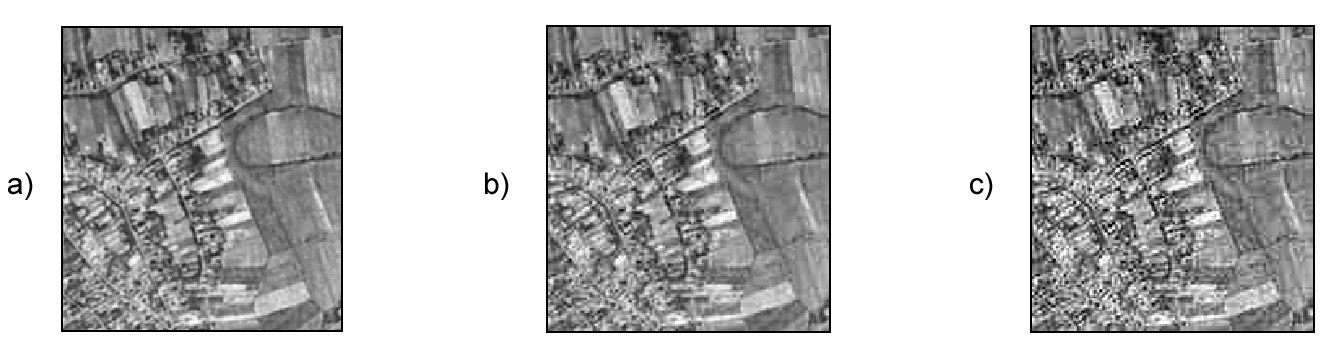
\includegraphics[width=.9\textwidth]{Fuentes_datos/Compresion_con_perdidas.png}
\caption{\small Efectos de la utilizaci�n de algoritmos de compresi�n con p�rdidas. a) Imagen original. b) Imagen almacenada mediante compresi�n con p�rdidas. c) Imagen tras diez procesos de lectura y almacenamiento en un formato de archivo con compresi�n con p�rdidas. El efecto de la degradaci�n sucesiva que la imagen sufre es claramente apreciable.}
\label{Fig:Compresion_con_perdidas} 
\end{figure}

\subsubsection{Formatos para datos SIG}

Junto con los formatos de archivo para im�genes, los SIG r�ster han desarrollado sus propios formatos para el almacenamiento de capas r�ster en general, y en particular de aquellas que no representan im�genes, tales como capas de variables f�sicas.

Estos formatos est�n pensados para las caracter�sticas de estas capas, que habitualmente recogen valores decimales (a diferencia de los valores enteros de los Niveles Digitales de una imagen), y que no suelen contener m�s que una �nica banda.

Adem�s de corresponder a un SIG particular (pr�cticamente cada SIG tiene su propio formato de archivo r�ster), otras aplicaciones que trabajan con este tipo de datos, tales como todas aquellas que usan por una u otra raz�n informaci�n de elevaciones, tambi�n disponen de sus formatos particulares. Muchos SIG pueden leer algunos de estos formatos junto con los suyos propios o los de otros SIG.

A la hora de almacenar una capa tal como un Modelo Digital del Terreno o cualquier otra de similar �ndole, estos formatos son preferibles en general a las im�genes, ya que los formatos de imagen, aunque ya hemos visto que pueden adaptarse y ser en algunos casos plenamente operativos para otro tipo de variables, no son formatos puramente pensados para este tipo de informaci�n.

\subsubsection{Principales formatos existentes}

Dentro de la gran variedad de formatos existentes, he aqu� una breve lista de los principales, los cuales suelen encontrarse con frecuencia a lo largo del desarrollo de un proyecto SIG habitual.

Dentro de los formatos para im�genes, cabe destacar los siguientes:

\begin{itemize}
	\item Tagged Image File Format (tif). Se trata de un formato complejo y altamente flexible, con muchas variantes distintas. Puede incorporar tanto compresi�n con p�rdidas como sin p�rdidas, en funci�n del algoritmo que se utilice. Se utiliza habitualmente tanto en el �mbito del tratamiento de im�genes como en el �mbito SIG. En este �ltimo, permite tambi�n el almacenamiento de valores decimales, siendo apto para almacenar capas que no representen im�genes como tal.
	Es un formato habitualmente generado por los esc�neres, con lo cual es frecuente su utilizaci�n al trabajar con cartograf�a escaneada, seg�n vimos antes en este mismo cap�tulo.
	Existe una variante denominada GeoTIFF, que permite incorporar en el propio fichero la georreferencia de la imagen, haciendo innecesario el uso de un \extr{World File} asociado.
	\item Joint Photographic Experts Group (jpg o jpeg). Un formato muy popular para im�genes (todas las c�maras digitales lo utilizan), no es sin embargo adecuado para el trabajo con SIG. Incorpora compresi�n con p�rdidas (el ejemplo de la figura \ref{Fig:Compresion_con_perdidas} ha sido realizado utilizando este formato), y no es apto para almacenar capas r�ster que no sean de tipo imagen.
\end{itemize}
\index{Tagged Image File Format (TIFF)}\index{Joint Photographic Experts Group (JPEG)}\index{GeoTIFF}

Algunos formatos espec�ficos para im�genes SIG tales como im�genes de sat�lite, son:

\begin{itemize}
	\item Enhanced Compression Wavelet (ecw). Formato desarrollado por Earth Resource Mapping. Al igual que el siguiente, est� especialmente preparado para almacenar im�genes de gran tama�o, ya que las im�genes a�reas o de sat�lite en general tiene tama�os mayores que las im�genes de uso gen�rico para las que est�n pensados los formatos como TIFF o JPEG. 
	En el uso de estas im�genes de gran tama�o en un SIG, es habitual que se quiera acceder a la imagen (por ejemplo para su visualizaci�n) solo en una parte determinada de la misma. Para optimizar este tipo de acceso, el formato soporta acceso sin necesidad de descomprimir la totalidad del archivo (descompresi�n selectiva).
	Se trata de un formato de compresi�n con p�rdidas, y su grado de compresi�n es alto. 
	\item Multi--resolution Seamless Image Database (MrSID) (sid). Al contrario que el anterior, que es un formato abierto, el formato MrSID es un formato cerrado, pero sus caracter�sticas son similares: alta compresi�n, preparado para im�genes de gran volumen y con posibilidad de descompresi�n selectiva.
\end{itemize}
\index{Enhanced Compression Wavelet (ECW)}\index{Multi--resolution Seamless Image Database (MrSID)}

Por �ltimo, entre los formatos para datos r�ster (no im�genes) m�s comunes destacar el siguiente:

\begin{itemize}
	\item ArcInfo ASCII (asc). Un formato en texto plano ASCII\footnote{\emph{American Standard Code for Information Interchange}. Un esquema de codificaci�n de caracteres ampliamente utilizado.}. �nicamente soporta una �nica banda, y permite almacenar el valor a considerar como valor de sin datos.
\end{itemize}
\index{ArcInfo ASCII (formato)}\index{American Standard Code for Information Interchange (ASCII)}

\subsection{Formatos para datos vectoriales}

Sin ser tan abundantes como los formatos para datos r�ster, existe tambi�n un buen n�mero de formatos de archivo para datos vectoriales. Al igual que en el caso r�ster, estos formatos de archivo no derivan �nicamente de los SIG, sino tambi�n de otras aplicaciones que utilizan capas de tipo vectorial, con  particular importancia de las de dise�o asistido por ordenador (CAD).

A la hora de definir las caracter�sticas de un formato de archivo para datos vectoriales, encontramos dos aspectos principales, a saber:

\begin{itemize}
	\item Capacidad para recoger la topolog�a de la capa
	\item Capacidad para recoger los atributos de las entidades.
\end{itemize}

En el primer aspecto, debemos considerar que existen SIG no topol�gicos, es decir, que no son capaces de manejar informaci�n sobre la topolog�a de la capa, y por tanto no la necesitan. Los formatos de archivo de estos SIG no estar�n por tanto pensados para trabajar con topolog�a, y por ello no la almacenan.

Respecto a la capacidad para recoger los atributos de una capa, este aspecto afecta principalmente a los formatos propios de las aplicaciones CAD. En estas, la componente espacial es la que prima, no teniendo tanta relevancia la componente tem�tica. Los puntos, l�neas y pol�gonos con los que se trabaja en un CAD no tiene atributos asociados salvo aquellos relacionados con su propia representaci�n tales como color, grosor o estilo. Existen formas de asociar una componente tem�tica a esas entidades, pero estas son variadas y la interoperabilidad disminuye en caso de emplearlas, ya que no est�n soportadas con car�cter general en los distintos SIG. 

Por esta raz�n, estos formatos son aptos para introducir informaci�n dentro de un SIG o para exportarla a un CAD con objeto de utilizar capacidades de este que no se tengan en el SIG, pero como formatos de almacenamiento de datos dentro de un SIG no son los m�s id�neos, y debe optarse por otros m�s espec�ficos para datos SIG.

\subsubsection{Principales formatos existentes}

Los formatos m�s extendidos para datos SIG vectoriales son los siguientes:

\begin{itemize}
	\item Shapefile (shp). Propuesto por la empresa ESRI, es el formato m�s utilizado en la actualidad, convertido en un est�ndar \emph{de facto}. No soporta topolog�a y se compone de diversos ficheros, cada uno de los cuales contiene distintos elementos del dato espacial (geometr�as, atributos, �ndices espaciales, etc.)
	\item MapInfo TAB. Un formato tambi�n popular, desarrollado con el software MapInfo, de la empresa del mismo nombre.	
\end{itemize}

\index{Shapefile}
\index{MapInfo TAB}\index{Estandar!de facto}

Los formatos de aplicaciones CAD son muy habituales tambi�n, destacando los siguientes:

\begin{itemize}
	\item DWG. El formato nativo de AutoCAD, la aplicaci�n m�s popular en el dise�o asistido por ordenador. Permite almacenar datos bidimensionales y tridimensionales, as� como metadatos. Se trata de un formato cerrado, y la lectura y escritura de este requiere el uso de  librerias facilitadas en condiciones determinadas por la empresa Autodesk, fabricante de Autocad y creador del formato. Aun as�, son muchas las aplicaciones que pueden leer archivos DWG.
	\item DXF. Tambi�n derivado de Autocad, surge para impulsar la interoperabilidad en el campo del CAD. En este caso no se trata de un formato cerrado, ya que Autodesk s� publica las especificaciones del formato. Aunque resulta de menos utilidad que el DWG pues no es capaz de almacenar los elementos m�s complejos que las �ltimas versiones de Autocad incorporan, a la hora de su empleo en un SIG como formato para el almacenamiento de cartograf�a resulta adecuado, y existe gran cantidad de datos cartogr�ficos en este formato.
	\item DGN. El formato nativo de otra aplicaci�n CAD muy extendida: MicroStation, de la empresa Intergraph.
\end{itemize}
\index{AutoCAD}\index{Autodesk}\index{DWG}\index{DXF}\index{MicroStation}\index{Intergraph}\index{DGN}

%A los anteriores deben a�adirse los formatos para el almacenamiento de bases de datos, las cuales estudiamos en el cap�tulo \ref{Bases_datos}.

\section{Resumen}

Los datos con los que trabajamos en un SIG pueden venir de muy distintas procedencias. Distinguimos aquellos que provienen directamente de alg�n tipo de medida o del empleo directo de alguna instrumentaci�n (fuentes de datos primarias), y otros que proceden de procesar un dato ya existente para adaptarlo a su uso en un SIG (fuentes de datos secundarias).

Una forma b�sica de crear datos espaciales digitales es la utilizaci�n de fuentes no digitales y su digitalizaci�n. Este proceso puede llevarse a cabo tanto de forma manual como automatizada, y puede dar como resultado tanto capas r�ster como capas vectoriales.

La teledetecci�n es una fuente de datos de gran importancia para los SIG. Dentro de ella se incluyen t�cnicas de muy diversa �ndole cuyos productos son muy distintos entre s�. El fundamento de la teledetecci�n es la medici�n de las propiedades de los objetos realizada sin que medie contacto con estos. Para ello, se emplean sensores que pueden ir a bordo de aviones o montados sobre sat�lites, y que pueden ser de tipo pasivo o activo. El resultado del proceso de teledetecci�n son im�genes con un n�mero variable de bandas, aunque tecnolog�as como el radar o el LiDAR pueden emplearse para la generaci�n de cartograf�a de elevaciones.

Dentro de las tecnolog�as que permiten la recogida de datos en campo, el GPS ha supuesto un cambio en la realizaci�n de este tipo de trabajos, y su integraci�n en SIG es sencilla. Esto les ha convertido en una fuente de datos muy utilizada en un gran n�mero de proyectos SIG.

Independientemente de su origen, los datos espaciales se almacenan en archivos cuyos formatos son a su vez muy variados. En este cap�tulo hemos visto algunos de los m�s habituales, as� como los aspectos m�s importantes que los definen, y que han de tenerse en cuenta a la hora de trabajar con dichos formatos y elegir los m�s adecuados.


\chapter{La calidad de los datos espaciales}\label{Calidad_datos}

\begin{keypoints}
�Cu�les son las principales fuentes de error en los datos espaciales?$\bullet$�C�mo pueden medirse esos errores? $\bullet$ �C�mo se gestiona el error dentro de un proyecto SIG? $\bullet$ �C�mo se propagan los errores existentes en los datos espaciales durante el trabajo con ellos en un SIG?
\end{keypoints} 

\bigskip

\begin{intro}
Todo dato espacial contiene alg�n tipo de error, en mayor o menor medida. Conocer las razones por las cuales aparecen esos errores es importante para poder evaluar correctamente la validez del trabajo que realizamos con los datos y los resultados que obtenemos a partir de ellos. En este cap�tulo se estudiaran los principales errores que pueden afectar a los distintos tipos de datos espaciales, las fuentes principales de dichos errores y las maneras en que estos pueden gestionarse dentro de un proyecto SIG.

Puesto que los datos son la materia prima para obtenci�n de nuevos datos a trav�s de los procesos y operaciones que dentro de un SIG realizamos con ellos, trataremos tambi�n la forma en que los errores en los datos de partida afectan a los resultados que derivemos de ellos.
\end{intro}

\section{Introducci�n}

Puesto que los datos son la base de todo el trabajo que realizamos en un SIG, su calidad es vital para que ese trabajo tenga sentido y aporte unos resultados coherentes y �tiles. Siendo la calidad el conjunto de propiedades y de caracter�sticas de un producto o servicio que le confieren su aptitud para satisfacer unas necesidades expl�citas e impl�citas \cite{AENOR1995}, desde el punto de vista del SIG unos datos espaciales de calidad ser�n aquellos que puedan servir para alcanzar los objetivos de un proyecto concreto, dando sentido a este. En este aspecto, se debe considerar la disposici�n de los datos \emph{per se}, aunque tambi�n las necesidades a las que pretendemos dar respuesta mediante los datos que utilizamos.

Por definici�n, ning�n dato es perfecto. Todo dato que utilicemos va a contener errores, y estos pueden ser desde totalmente irrelevantes para el desarrollo de un proceso de an�lisis hasta de tal magnitud que desvirt�en por completo los resultados de dicho an�lisis. Es importante no solo contar con datos de calidad en los que estos errores sean m�nimos, sino conocer el tipo de error que existe en nuestros datos y la magnitud de estos. Saber gestionar el error y ser consciente de las limitaciones de los datos de los que se dispone es importante para saber interpretar los resultados derivados del trabajo con dichos datos.

A lo largo de este cap�tulo veremos los aspectos m�s importantes que derivan de considerar el error como parte inevitable de nuestro trabajo con datos espaciales. Ello nos permitir� saber evaluar las capacidades de los datos para servir como punto de partida de nuestro trabajo, y a llevar este a cabo de la mejor manera posible, considerando que se trabaja simult�neamente con un conjunto de datos y con un error impl�cito asociado a estos.

\cite{Gomez2004Geofocus} apunta las siguientes etapas para la modelaci�n del error:

\begin{itemize}
	\item Identificaci�n de la fuente de error.
	\item Detecci�n y medida del error.
	\item Modelaci�n de la propagaci�n del error.
	\item Propuestas de estrategias para la gesti�n y reducci�n del error.
\end{itemize}

Ser� sobre estas distintas fases sobre las que trataremos en las pr�ximas secciones.

\section{La importancia de la calidad de los datos}

A pesar de su gran importancia, la calidad de los datos espaciales no ha sido una preocupaci�n hasta hace relativamente poco tiempo. Los textos sobre Sistemas de Informaci�n Geogr�fica tales como este mismo libro apenas trataban el tema en sus inicios \cite{Foote2000, Oort2005NGC}, y solo en la actualidad aparece una concienciaci�n acerca de la importancia que la calidad de los datos espaciales tiene sobre el desarrollo de cualquier trabajo basado en ellos.

Las razones por las que la calidad de los datos empieza a considerarse como un elemento de gran relevancia en el �mbito geogr�fico son principalmente dos \cite{Oort2005NGC}:

\begin{itemize}
	\item Aparici�n de los SIG.
	\item Amplio crecimiento del volumen de datos espaciales disponibles, especialmente los derivados de sat�lites.
\end{itemize}

Estos dos factores, inevitablemente unidos, han favorecido que el volumen de trabajo sobre datos espaciales sea mayor y que adem�s se use un n�mero m�s elevado de datos distintos. Es l�gico pensar que, a ra�z de esto, haya surgido el inter�s por evaluar y tratar de forma rigurosa las condiciones en las que estos trabajos se est�n llevando a cabo.

La preocupaci�n por la calidad de los datos es b�sica por el simple hecho de que datos de mala calidad generan invariablemente resultados de mala calidad. Utilizar un dato de mala calidad es equivalente a utilizar un modelo equivocado. Si el modelo no es cierto, no importa la buena calidad de los datos, ya que los resultados que arrojar� tampoco lo ser�n. Del mismo modo, un dato con un error superior al que puede resultar tolerable para una determinada tarea hace que la calidad de este sea insuficiente, y los resultados obtenidos carecen de valor.

A pesar de que la aparici�n de los SIG ha sido una de las razones principales para que se tenga en consideraci�n la calidad de los datos y se especifique formalmente el modo de tratarla y gestionarla, los SIG en s� no disponen apenas de herramientas para asistir en estas tareas. Aunque la ciencia de la informaci�n geogr�fica ha avanzado mucho en ese sentido, y el conocimiento relativo a la calidad de los datos espaciales es mucho mayor, los SIG no han incorporado ese conocimiento, y carecen de funcionalidades al respecto. Dicho de otro modo, existen las formulaciones y los elementos te�ricos, pero estos a�n no se han visto materializados (o lo han hecho de forma pr�cticamente anecd�tica) en los SIG de uso habitual. Por esta raz�n, la mayor�a de usuarios de SIG no tienen en cuenta rigurosa y formalmente la calidad de los datos a la hora de desarrollar su trabajo, quedando a�n mucho por avanzar en este sentido.

Un elemento clave para el control de la calidad es la existencia de metadatos,\index{Metadatos} que informan acerca de dichos datos sobre una serie de aspectos relativos a estos, entre ellos aquellos que afectan a la calidad. Los metadatos se tratan con gran profundidad dentro de este libro en el cap�tulo \ref{Metadatos}.


\section{Conceptos y definiciones sobre calidad de datos}

Antes de entrar en el estudio directo de la calidad de los datos espaciales y el estudio de los errores que pueden presentarse en un dato espacial, es necesario definir algunos conceptos b�sicos y alguna terminolog�a al respecto.

El concepto b�sico es el \emph{error}, que no es sino la discrepancia existente entre el valor real (puede ser un valor de posici�n, de un atributo, o cualquier otro), y el valor recogido en una capa. El error puede ser de dos tipos: \emph{sistem�tico} y \emph{aleatorio}. \index{Error}

Dos t�rminos importantes en el estudio de la calidad son la \emph{precisi�n} y \emph{exactitud}. La precisi�n indica el nivel de detalle con el que se recoge la informaci�n. Un capa en la que las posiciones se han medido con 5 valores decimales es m�s precisa que una en la que se han medido con un �nico decimal. \index{Precisi�n}\index{Exactitud}

Dependiendo del uso que se pretenda dar a una capa de datos geogr�ficos, se requerir� una u otra precisi�n. Un trabajo geod�sico requerir� medir la localizaci�n de un punto con precisi�n milim�trica, mientras que para un muestreo para inventario forestal es suficiente localizar las parcelas correspondientes con una precisi�n mucho menor.

Por su parte, la exactitud nos indica el grado en que los valores estimados se asemejan al valor real. 

La exactitud se calcula con el error sistem�tico, mientras que la precisi�n se calcula a partir del error aleatorio. Existe una relaci�n directa entre precisi�n y exactitud, y en ocasiones se emplean ambos t�rminos indistintamente. Si no existen errores sistem�ticos (no existe un sesgo), la precisi�n y la exactitud son iguales.

Es posible, no obstante, que un dato sea muy preciso pero poco exacto, ya que las magnitudes de los distintos tipos de errores pueden ser muy distintas. Este hecho puede verse claramente en la figura \ref{Fig:Imprecision_exactitud}.

\begin{figure}[!hbt]
\centering
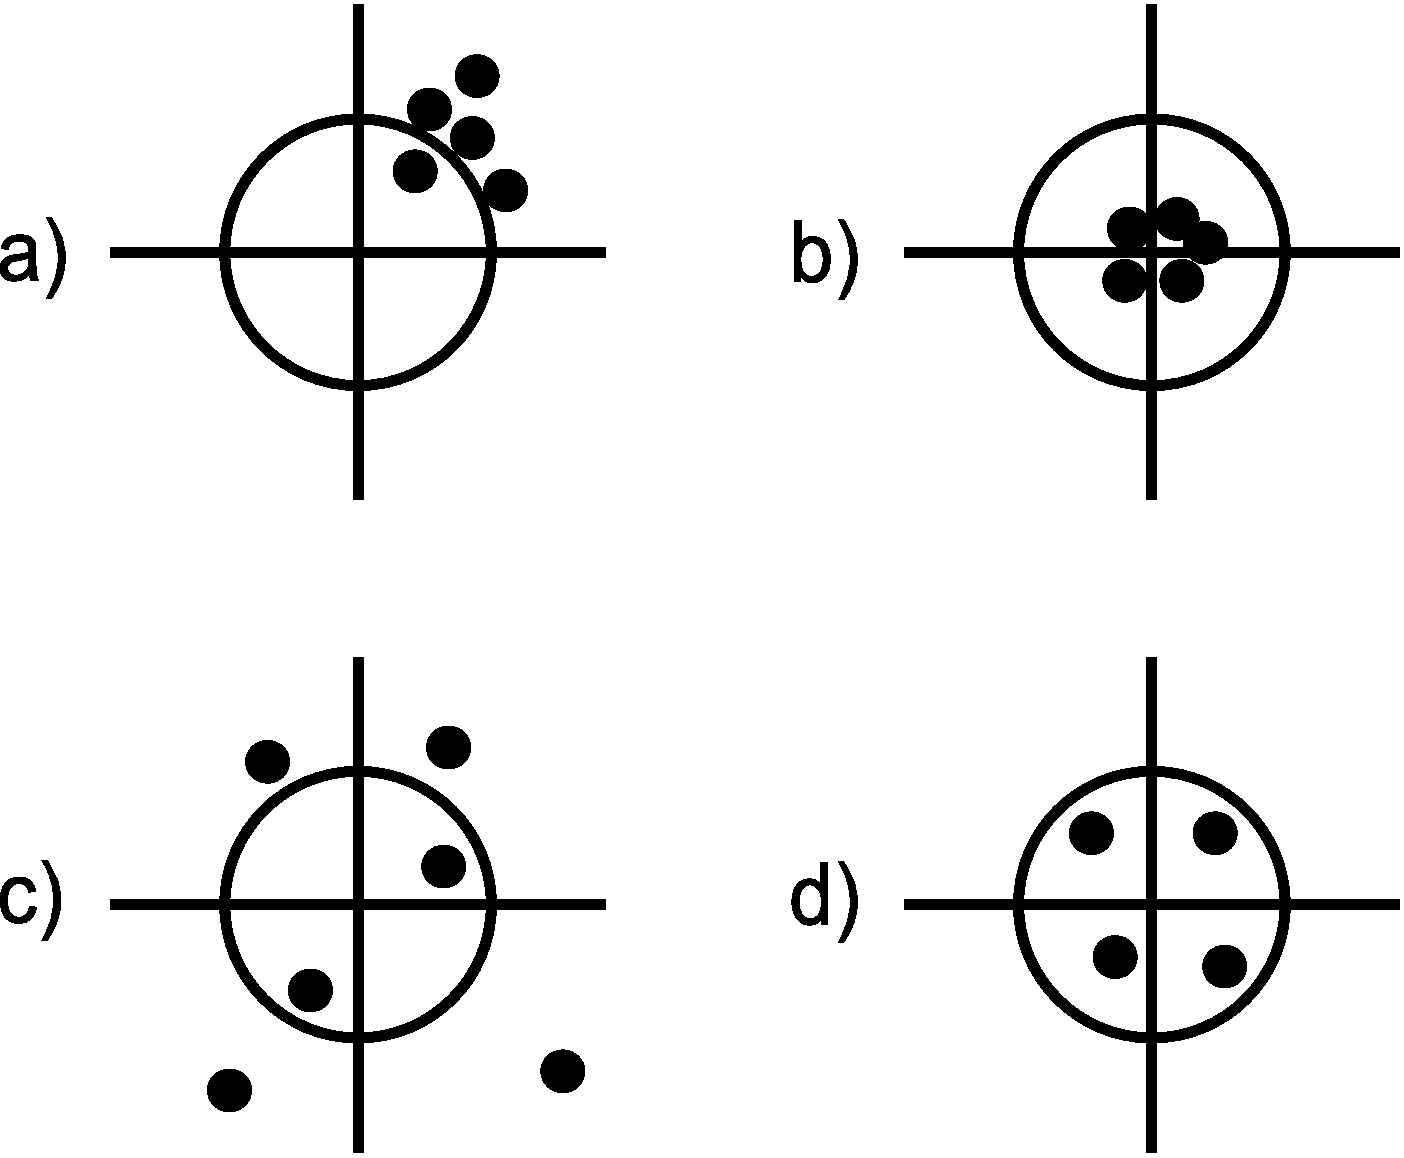
\includegraphics[width=.5\textwidth]{Calidad_datos/Imprecision_exactitud.pdf}
\caption{\small Diferencia entre precisi�n y exactitud (Tomado de \cite{Heywood1998Longman}). En a) y b) la precisi�n es elevada, mientras que en c) y d) es baja. Por su parte, en a) y c) la exactitud es baja, siendo alta en b) y d).}
\label{Fig:Imprecision_exactitud}
\end{figure}

Por �ltimo, un par�metro relativo al error es la \emph{incertidumbre}. Habitualmente, el valor real es desconocido, por lo que el error no puede conocerse. La incertidumbre refleja la medida en que no podemos tener certeza de la validez de nuestros datos. La incertidumbre es un concepto m�s amplio que el error, y auna tres componentes \cite{Fisher1999Wiley}:\index{Incertidumbre}

\begin{itemize}
	\item Error
	\item Vaguedad. Aparece como consecuencia de definiciones pobres o incompletas, as� como cuando los objetos que se modelizan en los datos no presentan l�mites bien definidos. Por ejemplo, en una capa de clases de vegetaci�n, la transici�n entre una clase y otra se produce normalmente de forma gradual, por lo que el establecimiento de una frontera brusca es un hecho artificial que aumenta la incertidumbre, y el significado de que un punto en concreto se asigne a una clase dada es m�s vago cuanto m�s cerca de esa frontera nos encontramos.
	\item Ambig�edad. Cuando no existen definiciones inequ�vocas de los conceptos fundamentales, aparecen ambig�edades que a�aden igualmente incertidumbre al dato creado en funci�n de estos. 
\end{itemize}\index{Vaguedad}\index{Ambig�edad}

Tradicionalmente se ha trabajado con el error y no con el concepto de incertidumbre, pero conocer esta es igualmente importante a la hora de evaluar la calidad de los datos, y la modelizaci�n de la incertidumbre es una alternativa a la modelizaci�n del error.

\section{Fuentes y tipos de errores}
\index{Error!fuentes}

Cuando un dato espacial llega a nosotros para ser empleado en un SIG, ha pasado por una serie de etapas a lo largo de los cuales puede haber incorporado errores. Estudiando esas etapas por separado, encontramos las siguientes fuentes de error \cite{Heuvelink1998Taylor, Heywood1998Longman}:

\begin{itemize}
	\item Errores de concepto y modelo. Al recoger la informaci�n espacial utilizamos alg�n modelo de representaci�n (r�ster, vectorial), el cual siempre tiene alguna deficiencia. La realidad y las tareas que pretendemos realizar con una capa de informaci�n espacial no se adaptan por completo a ninguno de los modelos de representaci�n, y el hecho de optar por uno u otro conlleva la introducci�n de alg�n error, o condiciona para la aparici�n de unos u otros errores en las etapas posteriores.
	\item Errores en las fuentes primarias. El dato vectorial del que disponemos proviene originariamente de una fuente primaria, la cual puede contener errores. Si esta fuente contiene errores, estos aparecer�n tambi�n en los datos que se deriven de este. As�, si digitalizamos en base a un mapa escaneado y la hoja original es err�nea, tambi�n lo ser�n las capas que creemos en esa digitalizaci�n.
	\item Errores en los procesos de creaci�n de la capa. Los procesos que realizamos para crear la capa pueden incorporar errores en el resultado. Por ejemplo, en el proceso de digitalizaci�n\index{Digitalizaci�n} en base a ese mapa escaneado pueden aparecer errores por razones tales como un mal trabajo del operario, ya sea al digitalizar las entidades sobre una tableta o al teclear los valores de los atributos.
	Otros procesos, como pueden ser los de conversi�n entre los modelos r�ster y vectorial, tambi�n pueden tener como consecuencia la aparici�n de errores. Los cap�tulos \ref{Creacion_capas_raster} y \ref{Creacion_capas_vectoriales} tratan estos procesos de conversi�n, y se ver� en su momento los posibles errores que pueden aparecer en cada caso y las razones por las que lo hacen. Igualmente, se ver� como aplicar a esos procesos los elementos de medida del error que se desarrollar�n m�s adelante en este cap�tulo.
	\item Errores en los procesos de an�lisis. Un dato espacial puede derivar de un proceso de an�lisis, y en �l pueden aparecer errores debidos principalmente a dos razones: o bien la capa original objeto de an�lisis contiene de por s� errores, o bien el proceso no es por completo correcto.
	Veremos en el cap�tulo \ref{Geomorfometria} c�mo a partir de un MDE podemos calcular una capa con valores de pendiente, y c�mo existen varios algoritmos distintos para realizar este c�lculo. Ninguno de esos algoritmos es completamente preciso, y los valores calculados presentaran discrepancias de distinta magnitud con el valor real de pendiente, en funci�n de diversos factores.
	Por su parte, el propio MDE tambi�n tiene sus propios errores, y estos se propagan a los resultados que derivamos de �l, como veremos m�s adelante con detalle.
	En la parte de procesos veremos muchas operaciones que van a generar nuevos datos espaciales, y que pueden implicar la aparici�n de errores. Trataremos estos en su momento en la medida que ello pueda ser relevante para el manejo y utilizaci�n de esos datos derivados.
\end{itemize}

\subsection{Las componentes de la calidad}

La calidad de un dato espacial depende de muchos factores. Las caracter�sticas que dotan de dicha calidad al dato espacial son variadas, pues el dato espacial es en s� complejo, y cada una de estas caracter�sticas es susceptible de incorporar errores y por tanto de implicar una p�rdida de calidad por ello. Las siguientes san algunos de los componentes principales de la calidad del dato espacial \cite{Oort2005NGC}:

\begin{itemize}
	\item Exactitud posicional. Todo dato espacial tiene asociada una referencia geogr�fica. La precisi�n con la que se toma esta condiciona la calidad del dato.
	Esta precisi�n puede considerarse �nicamente en los ejes $x$ e $y$, o tambi�n en el eje $z$ (elevaci�n). Esta �ltima, no obstante, puede considerarse como un atributo si se trabaja en un SIG bidimensional, y tratarse de la misma forma que cualquier otra variable de similar �ndole sin significado espacial, tal como la temperatura en el punto ($x,y)$ en cuesti�n.
	\item Exactitud en los atributos. Si la componente espacial puede tener errores, estos tambi�n pueden aparecer en la componente tem�tica. Los valores asociados a una coordenada u objeto espacial pueden haber sido medidos con m�s o menos exactitud, o presentar valores incorrectos por muy diversas causas.
	Cuando el atributo en cuesti�n es de tipo categ�rico, puede existir un error de clasificaci�n (se asocia la entidad espacial a una categor�a err�nea), mientras que en el caso de atributos no categ�ricos pueden sencillamente aparecer valores mayores o menores que los reales.
	\item Consistencia l�gica y coherencia topol�gica. Los datos espaciales no son elementos independientes, sino que existen relaciones entre ellos. Un dato de calidad debe recoger fielmente estas relaciones, siendo la topolog�a la encargada de reflejar este tipo de informaci�n. Por ello, debe existir una coherencia topol�gica en el dato espacial.
	Adem�s de la coherencia de las relaciones, existe una coherencia impl�cita en todo atributo o valor recogido, de forma que resulte l�gico. Estos atributos y valores han de ser coherentes con las escalas de medida o el tipo de valor que se espera, entre otros. As� un valor de elevaci�n no puede ser igual a ``suelo calizo'', ni un valor de temperatura expresado en Kelvin igual a -87.
	\item Compleci�n. El dato espacial no recoge todo lo que existe en una zona dada. Algunos elementos pueden no haberse recogido por cuestiones de escala (menores de un tama�o m�nimo), pero tambi�n pueden incluirse o excluirse en funci�n de otros criterios, en especial para el caso de mapas tem�ticos. Estos criterios deben conocerse para saber por qu� un dato espacial contiene una serie de valores o elementos y no otros.
	\item Calidad temporal. Aunque los datos espaciales son <<im�genes>> est�ticas de la realidad, el tiempo es importante en muchos sentidos, pues afecta directamente a su calidad. La realidad que representa un dato geogr�fico es una realidad que var�a con el paso del tiempo, y por tanto este paso del tiempo puede degradar la calidad del dato espacial en mayor o menor medida.
	\item Procedencia. Un dato espacial puede provenir de una fuente m�s o menos fiable, o haber sido generado a trav�s de uno o varios procesos, en cada uno de los cuales se puede haber introducido alg�n tipo de error. Conocer la procedencia de un dato y los procesos que se han empleado en su confecci�n es necesario para poder evaluar su calidad.
\end{itemize}\index{Compleci�n}

Es importante recalcar que los errores que pueden incorporarse en estas componentes de la calidad pueden ser tanto de tipo cuantitativo como de tipo cualitativo, y que ello no est� necesariamente ligado a la naturaleza de la componente o el tipo de variable a la que esta hace referencia. As�, un error en un atributo de tipo categ�rico supone un error cualitativo, pero un error posicional en la componente $z$ (o de atributo de tipo continuo, si lo consideramos como tal) tambi�n puede dar lugar a un error cualitativo, como se muestra en la figura \ref{Fig:Error_cualitativo_elevacion}.

\begin{figure}[!hbt]
\centering
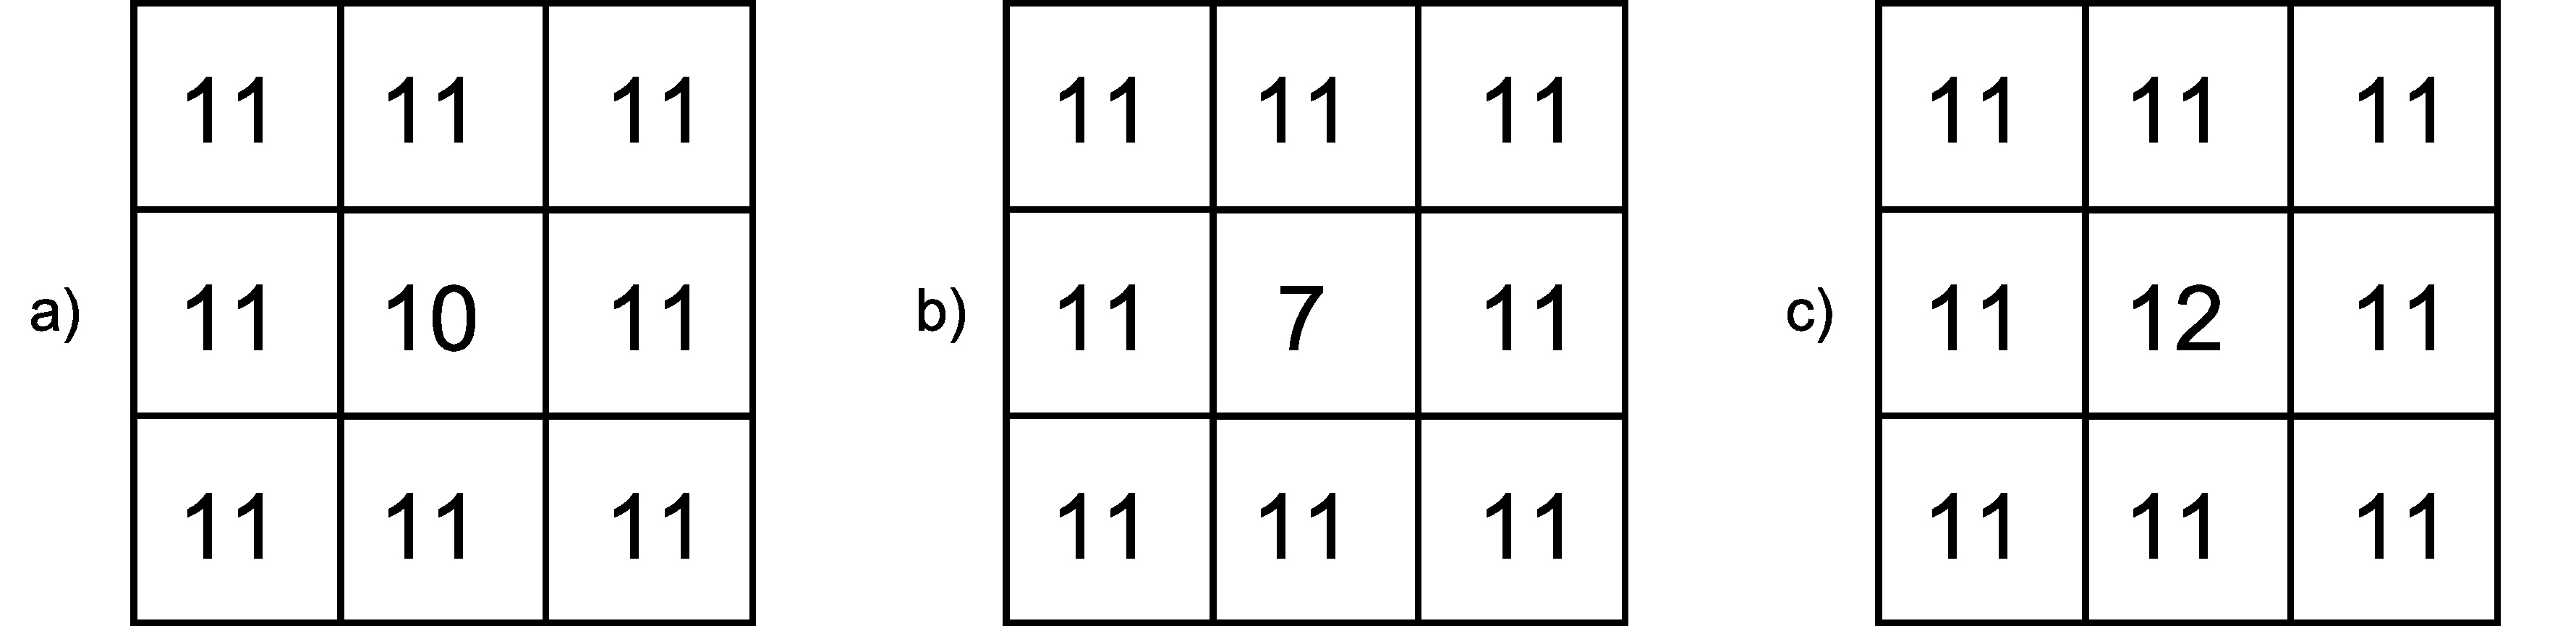
\includegraphics[width=.75\textwidth]{Calidad_datos/Error_cualitativo_elevacion.pdf}
\caption{\small a) MDE con valores reales. b) y c) Dos MDE con errores posicionales en $z$. En el caso c), el error no solo es cualitativo, sino tambi�n cuantitativo, ya que modifica la forma del terreno, pasando de ser una depresi�n a ser un pico.}
\label{Fig:Error_cualitativo_elevacion}
\end{figure}

En la figura, que representa una porci�n de un Modelo Digital de Elevaciones y dos variantes alternativas con sendos errores de medici�n de la elevaci�n, en el primer caso, y pese a que el error es mayor (hay mayor discrepancia entre el valor real y el recogido en el MDE), no var�a la configuraci�n del terreno. En la celda central encontramos una depresi�n, ya que en ella la elevaci�n es menor que en las circundantes, y esto sigue ocurriendo as� a pesar de existir ese error posicional. En el segundo caso (subfigura c), sin embargo, el error es menor en magnitud, pero al ser de signo contrario hace que la depresi�n se convierta en un pico, una configuraci�n del terreno exactamente inversa. Si estudiamos las formas del terreno en ese punto (un an�lisis que arroja resultados cualitativos), obtendremos un valor err�neo. \index{Modelo Digital de Elevaciones}

Veremos m�s adelante que este tipo de errores son de gran importancia para muchos an�lisis, en particular para los relacionados con el comportamiento hidrol�gico del terreno, que estudiaremos en el cap�tulo \ref{Geomorfometria}.

La forma en que los distintos tipos de errores aparecen en una capa es diferente en funci�n del modelo de representaci�n empleado, ya que cada uno de estos modelos tiene sus propias debilidades, y las fuentes de datos de las que pueden proceder son asimismo distintas.

As�, los errores posicionales son m�s comunes en el caso de capas vectoriales, y una de las fuentes de error principal en este sentido son los procesos de digitalizaci�n, especialmente si son de tipo manual. Junto a los errores de digitalizaci�n que vimos en el cap�tulo \ref{Fuentes_datos} (v�ase la  figura \ref{Fig:Imprecisiones_digitalizacion}), existen otros que pueden aparecer al crear una capa vectorial, tales como los que se muestran en la figura \ref{Fig:Errores_digitalizacion} para el caso de digitalizar una l�nea.\index{Digitalizaci�n}

\begin{figure}[!hbt]
\centering
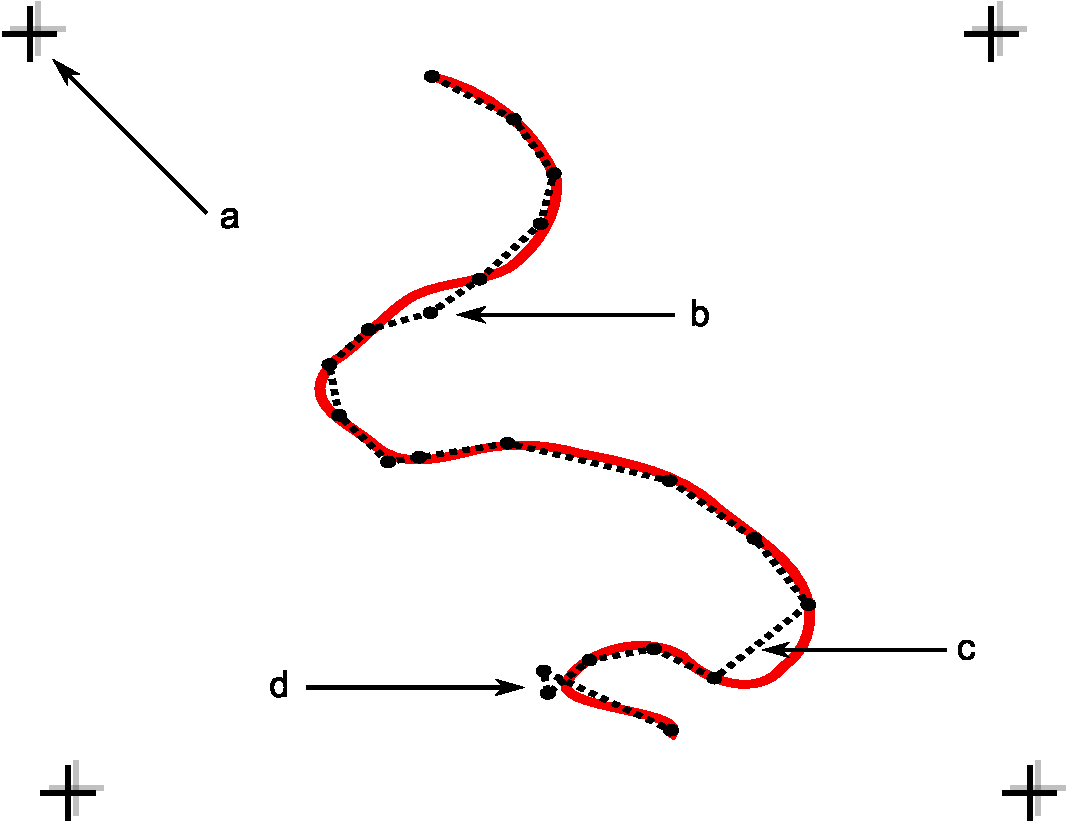
\includegraphics[width=.5\textwidth]{Calidad_datos/Errores_digitalizacion.pdf}
\caption{\small Algunos errores que aparecen en la digitalizaci�n de lineas. a) Registro inexacto, b) puntos mal situados, c) desplazamientos por v�rtices insuficientes, d) errores de registro.}
\label{Fig:Errores_digitalizacion}
\end{figure}

Con independencia de la pericia y experiencia de un operador, resulta imposible que sea capaz de reproducir exactamente el objeto original y trazar con el cursor de la tableta digitalizadora o el rat�n todos los detalles de este con absoluta fidelidad. Entre los errores que pueden aparecer encontramos falsos nudos (intersecciones de una l�nea consigo misma que no existen en realidad), puntos situados fuera del objeto, coincidencia imperfecta entre pol�gonos o mala referenciaci�n de la hoja al situarla sobre la tableta (en el proceso de registro).

El problema principal en el caso de digitalizar l�neas o pol�gonos (que pueden causar la aparici�n de mayor n�mero de errores por su mayor complejidad) estriba en que aquello que se digitaliza es un conjunto infinito de puntos, y el proceso de digitalizaci�n solo puede recoger un n�mero finito de ellos y despu�s unirlos mediante segmentos rectil�neos.

La componente tem�tica de una capa vectorial tambi�n puede adolecer de errores, que derivan a su vez tanto del proceso de introducci�n de los mismos como de los procesos de medici�n mediante los que se ha obtenido el valor concreto. 

En el caso de capas r�ster, sin embargo, existen algunas fuentes de error que tienen menor importancia, mientras que otras s� han de tenerse en cuenta por su relevancia. Por ejemplo, la introducci�n de la componente tem�tica en una capa vectorial puede hacerse manualmente con el teclado, mientras que en el caso de una capa r�ster los valores de las celdas no se introducen manualmente.

Ello no significa que las capas r�ster no presenten errores en sus valores, pero el origen de estos es diferente. Un error habitual aparece en capas con informaci�n categ�rica que proceden de la clasificaci�n de im�genes a�reas o de sat�lite. Los procesos que clasifican cada p�xel de la imagen en funci�n de sus Niveles Digitales (los cuales veremos en el cap�tulo \ref{Estadistica_avanzada}) introducen frecuentemente errores, y aparecen p�xeles mal clasificados cuyo valor de clase no es correcto.\index{Pixel}

Los errores posicionales se presentan de forma distinta a lo mostrado en la capa \ref{Fig:Errores_digitalizacion}. Las entidades tales como l�neas van a tener una representaci�n err�nea debido a la resoluci�n de la capa r�ster, que no va a permitir registrar con fidelidad su forma real. Por otra parte, la georreferenciaci�n de una imagen incorpora asimismo errores, que son equivalentes al error de registro en la digitalizaci�n vectorial. Este error va a ser distinto seg�n las zonas de la imagen, ya que la distorsi�n que implica la transformaci�n realizada no supone un error constante. Veremos estas funciones con m�s detalle tambi�n en el cap�tulo \ref{Procesado_imagenes}, donde se tratan los dos principales errores que afectan a las im�genes: errores geom�tricos y errores radiom�tricos (b�sicamente, errores posicionales y errores en los Niveles Digitales).\index{Digitales}

Adem�s de los errores de un �nico dato espacial (una capa de informaci�n), es importante considerar la forma en que los errores de distintos datos interact�an entre s�. En el trabajo con SIG es raro emplear una �nica capa, y lo m�s frecuente es trabajar con varias de ellas coordinadamente, cada una con sus respectivos errores. El modo en que esos errores se afectan entre s� puede condicionar la calidad de los resultados de forma similar a como los propios errores como tales lo hacen.

Como muestra la figura \ref{Fig:Sinergia_errores}, dos errores sistem�ticos de igual magnitud en sendas capas pueden tener efectos distintos sobre el resultado dependiendo de sus signos.

\begin{figure}[!hbt]
\centering
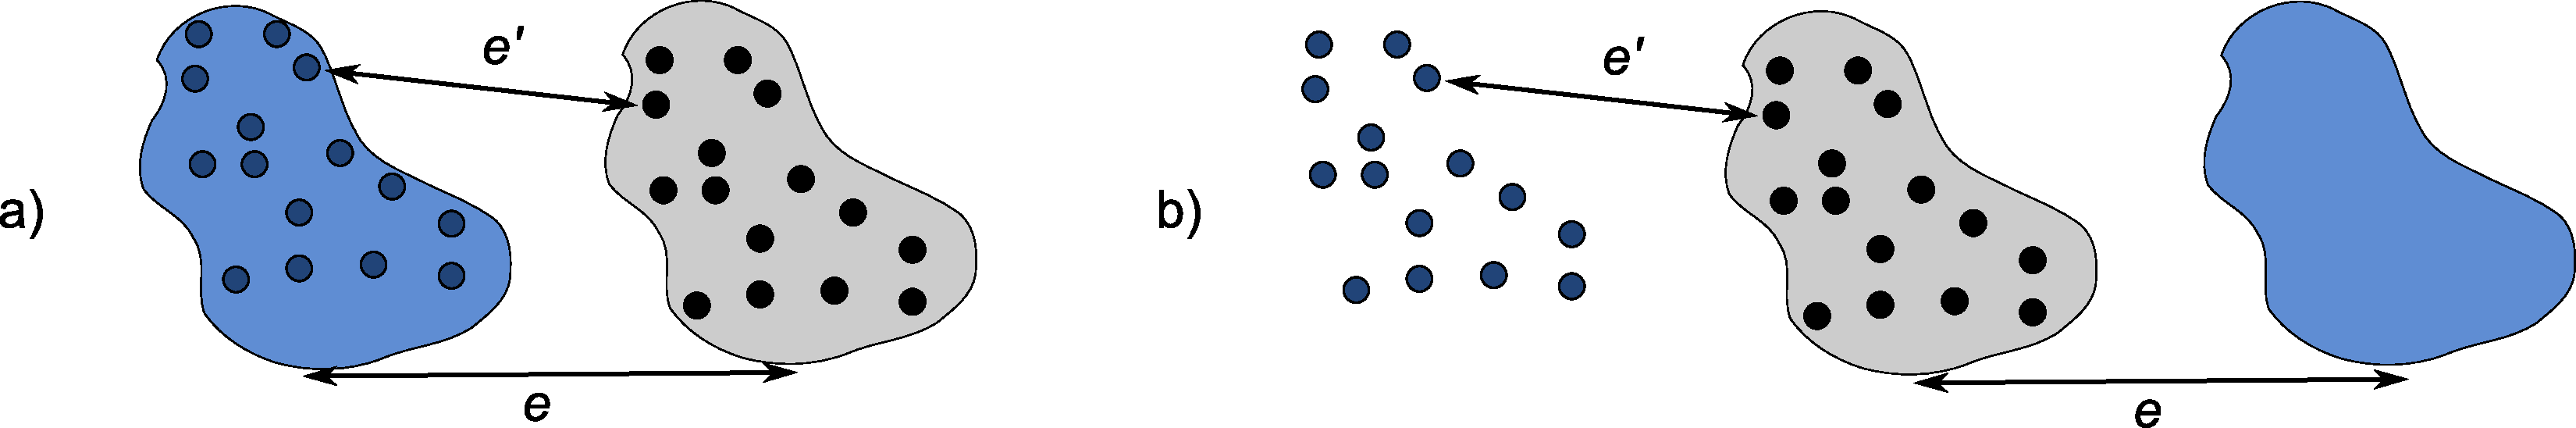
\includegraphics[width=.95\textwidth]{Calidad_datos/Sinergias_errores.pdf}
\caption{\small Un error $e$ pueden tener distintas consecuencias seg�n interact�en con los errores de otros datos espaciales ($e'$). En a) los errores casi se anulan, mientras que en b) se suman y dan lugar a un resultado err�neo. Los elementos en negro y gris indican la posici�n real.}
\label{Fig:Sinergia_errores}
\end{figure}

En la figura, tanto la capa de puntos como la de pol�gonos presentan un error sistem�tico. No obstante, un an�lisis que cuente el n�mero de puntos dentro del pol�gono seguir� dando el mismo resultado en uno de los casos, ya que la forma de los errores de ambas capas hace que estos no afecten a este an�lisis, mientras que en el otro caso el resultado es completamente distinto del real.

\section{Detecci�n y medici�n de errores}

Ahora que conocemos las fuentes y tipos de error, la evaluaci�n y tratamiento de este empieza por su localizaci�n para saber a qu� elementos del dato espacial afecta. Existen diversas metodolog�as para <<inspeccionar>> un dato espacial en busca de errores, que van desde m�todos sencillos y obvios hasta avanzadas t�cnicas con base estad�stica para detectar patrones particulares o elementos <<sospechosos>> de contener alg�n error.

La forma m�s sencilla es la mera exploraci�n visual. Algunos errores resultan obvios y una inspecci�n sencilla permitir� localizarlos sin dificultad. Una coincidencia deficiente entre pol�gonos dejar� un espacio en blanco que, si es de tama�o suficiente, puede ser localizado sencillamente en una exploraci�n visual. De igual modo sucede con otro tipo de errores, en particular los errores de posici�n tales como los falsos nudos o la aparici�n de formas <<il�gicas>> (calles con �ngulos muy bruscos, por ejemplo).

Es importante en este sentido que la representaci�n del dato espacial sobre la que se realiza la exploraci�n visual sea clara y adecuada, para revelar de la forma m�s notoria posible las posibles deficiencias de este. En este libro se dedica una parte entera a la visualizaci�n y representaci�n de la informaci�n espacial y, al contrario de lo que pueda pensarse, esta no es solo de importancia para la generaci�n de resultados al final de un flujo de trabajo, sino desde su mismo inicio. El an�lisis visual de los datos de partida, as� como otros procesos de an�lisis, pueden beneficiarse de una representaci�n correcta.

Existen errores que pueden detectarse visualmente, pero cuya detecci�n (y correcci�n) puede automatizarse. Errores de este tipo son, por ejemplo, las conexiones imprecisas entre segmentos, que ya vimos en el cap�tulo \ref{Fuentes_datos}. La funci�n de \emph{snapping} (ajuste por tolerancias), que se utiliza a la hora de digitalizar una capa vectorial, puede aplicarse \emph{a posteriori}, una vez que la capa ya ha sido digitalizada. El SIG puede buscar esos enlaces imperfectos y convertirlos en enlaces correctos, resolviendo las uniones en las que exista una distancia entre v�rtices menor que una tolerancia preestablecida.\index{Snapping}

Como sabemos, hay SIG que son capaces de manejar topolog�a y otros que no. Tambi�n hay formatos de archivo que pueden almacenar topolog�a y otros que no est�n pensados para ello. Por esta raz�n, los SIG topol�gicos trabajan a menudo con datos sin topolog�a, pero a partir de los cuales puede crearse esta, e implementan por ello las funciones para dicha creaci�n de topolog�a. Esta creaci�n implica la correcci�n de errores topol�gicos que puedan existir en los datos originales, que no son relevantes en el caso de no trabajar con topolog�a, y por ello pueden no haber sido detectados o eliminados. Errores como las antedichas falsas conexiones o los pol�gonos con adyacencia imperfecta, ambos se pueden corregir de forma autom�tica, formando parte esas funciones de correcci�n de las rutinas de creaci�n de topolog�a.\index{Topolog�a}

Otros errores no pueden detectarse visualmente, en muchos casos porque los motivos del error no se representan y no aparecen en la visualizaci�n. Errores topol�gicos relativos a las estructuras de datos empleadas para recoger dicha topolog�a entran en este grupo. En muchos casos, pueden no obstante corregirse de forma autom�tica a trav�s de operaciones de \emph{filtrado} y \emph{limpieza}, que se encargan de controlar la coherencia topol�gica del dato.

En el terreno de los atributos, la detecci�n de errores puede llevarse a cabo empleando las t�cnicas estad�sticas habituales. La detecci�n de valores improbables (\extr{outliers}) es uno de los procesos b�sicos. Estos \extr{outliers} son observaciones dentro de un conjunto de datos que no parecen guardar consistencia con el resto del conjunto \cite{Barnett1995Wiley} y cuya detecci�n puede llevarse a cabo de modo anal�tico o bien de modo visual, representando gr�ficamente los valores de los atributos. En general, las metodolog�as se fundamentan en comparar los valores con una distribuci�n te�rica y detectar la discordancia con esa distribuci�n. Formas automatizadas de detectar \extr{outliers} pueden encontrarse en \cite{LastOutliers}.\index{Outlier}

Observaciones de este tipo, alejadas de las caracter�sticas generales del conjunto de datos, pueden derivar de medidas err�neas tales como las provocadas por un equipo de medici�n en mal estado, aunque tambi�n pueden representar valores correctos pero de car�cter excepcional. 

Si se combina la componente espacial con la componente tem�tica encontramos otro tipo de valores inusuales, los denominados \emph{outliers espaciales}. Estos se definen como observaciones que son discordantes con las observaciones realizadas en su vecindad\footnote{Este hecho tiene relaci�n con el concepto de \emph{autocorrelaci�n espacial}, que veremos en detalle en el cap�tulo \ref{Analisis_espacial}, y que expresa la idea l�gica de que las mediciones cercanas deben tener valores similares} \cite{Lu2003IEEE}. \index{Outlier!espacial}

La diferencia entre un \extr{outlier} en la componente tem�tica y un \extr{outlier} espacial es clara. As�, un valor de 10000 metros en elevaci�n constituye siempre un valor excepcional, ya que va a encontrarse lejos de los valores medios recogidos, independientemente del lugar donde se hayan efectuado las mediciones. Un valor de 5000 metros puede constituir un \extr{outlier} espacial en unas zonas (si tomamos medidas de elevaci�n en, por ejemplo, Madrid, ya que ser� muy distinto del resto de elevaciones), pero puede ser un valor perfectamente l�gico en otras zonas de estudio.

La detecci�n de este tipo de valores puede realizarse, al igual que en el caso no espacial, de forma anal�tica o bien mediante exploraci�n visual.

En base a lo anterior, existen una serie de procedimientos y metodolog�as para la detecci�n de valores il�gicos en un juego de datos, los cuales se dividen de forma m�s gen�rica en dos grupos principales: unidimensionales y multidimensionales. Cuando en los multidimensionales la vecindad se define �nicamente en funci�n de la localizaci�n espacial y sin utilizar la componente tem�tica, se tiene la detecci�n de \extr{outliers} espaciales. La figura \ref{Fig:Deteccion_outliers} muestra un esquema de esta clasificaci�n y las metodolog�as m�s habituales. En \cite{Shekhard2003Unified} puede encontrarse m�s informaci�n al respecto.

\begin{figure}[!hbt]
\centering
\includegraphics[width=.7\textwidth]{Calidad_datos/Deteccion_outliers.pdf}
\caption{\small Clasificaci�n de m�todos para la detecci�n de observaciones inconsistentes \extr{(outliers)}}
\label{Fig:Deteccion_outliers}
\end{figure}


Una vez localizado el error, este puede cuantificarse de diversas formas, seg�n sea la naturaleza de la variable sobre la que se produce dicho error. 

Los errores posicionales o los atributos no categ�ricos son variables de tipo cuantitativo. El \emph{Error Medio Cuadr�tico} es la forma m�s habitual de medir esos errores. Su expresi�n es:\index{Error!Medio Cuadr�tico}

\begin{equation}
\mathrm{EMC}= \sqrt{\sum_{i=1}^N{\frac{(y_i - y_i')^2}{N}}}
\end{equation}

\noindent donde $N$ es el total de puntos en los que se comprueba el error, $y$ el valor real, e $y'$ el valor estimado. En esencia, se trata de una desviaci�n t�pica, por lo cual se asume al emplear esta medida que los errores son aleatorios y se distribuyen normalmente.

Otras medidas utilizadas son el \emph{Error Medio}, el \emph{Error Medio Absoluto} o el \emph{Error M�ximo}.

Para valores cualitativos no puede aplicarse esta medida, y deben emplearse otros par�metros. La medida del n�mero de valores que coinciden (elementos correctamente atribuidos) es una forma de determinar el error existente. El uso de la \emph{matriz de confusi�n} es la forma m�s habitual de medir el error en la componente tem�tica cuando esta es de tipo cualitativo. Veremos con m�s detalle su empleo y el de otras t�cnicas m�s complejas de similar prop�sito en el apartado \ref{Validacion}.\index{Matriz! de confusi�n}

\section{Propagaci�n de errores y modelaci�n del error}

El an�lisis de un dato espacial con errores va a dar un resultado que contiene a su vez errores, y existir� una relaci�n directa entre los errores en el dato de partida y aquellos que aparecen en el dato resultante de su an�lisis. Este hecho se conoce como \emph{propagaci�n de errores}.

\index{Error!Propagaci�n}

La propagaci�n de errores puede ser muy variable en funci�n del tipo de error que aparezca y la clase de an�lisis que se lleve a cabo. Errores de gran magnitud en el dato original pueden no tener apenas efecto en el resultado, mientras que peque�os errores pueden causar grandes alteraciones en la calidad del resultado \cite{Hengl2008Elsevier}.

Una de las �reas en las que m�s se ha trabajado en el estudio de la propagaci�n de errores es el trabajo con Modelos Digitales de Elevaciones. Como veremos en el cap�tulo \ref{Geomorfometria}, los MDE son un dato de primer orden, ya que resultan de utilidad en pr�cticamente cualquier tipo de proyecto SIG, y son muy numerosos los distintos par�metros que podemos derivar de ellos. Por esta raz�n, la propagaci�n de errores es un asunto importante dentro del trabajo con un MDE, pues de �l se van a obtener muchos datos nuevos, e interesa saber c�mo la calidad de estos nuevos datos se va a ver afectada por la calidad del MDE de partida.

El error principal que se estudia en este tipo de an�lisis en un MDE es el de los atributos, es decir, el de la elevaci�n. Los datos empleados se basan en el modelo de representaci�n r�ster, ya que este es el m�s habitualmente empleado para los an�lisis de un MDE. No obstante, metodolog�as como la que veremos a continuaci�n pueden aplicarse igualmente para la modelaci�n de otros errores, tales como los errores posicionales en la digitalizaci�n de una capa vectorial.

La metodolog�a m�s extendida para la modelaci�n de errores es la basada en simulaciones de Monte Carlo. El fundamento de este m�todo es considerar un dato espacial dado (un MDE para el caso de este ejemplo) como una de las posibles <<versiones>> de la realidad que pueden existir con una magnitud de error concreta. Evaluando el error existente en un dato espacial y su distribuci�n, y realizando simulaciones estoc�sticas en base a este, pueden obtenerse otras de esas <<versiones>> de la realidad. Posteriormente, puede realizarse el an�lisis no sobre el MDE con tal, sino sobre todo ese conjunto de datos derivados del MDE y su distribuci�n de error.\index{Monte Carlo}

De este modo, se simula la presencia de error a�adiendo ruido al MDE original, pero de una forma acorde con el propio error existente en el dato base. De las alternativas que se obtienen mediante estas simulaciones, ninguna de ellas tiene que ser necesariamente correcta y carente de errores \cite{Chrisman1989Autocarto} (lo m�s probable es que ninguna lo sea), pero el conjunto define un intervalo probable en el cual se situar�n los valores reales. Se modela as� la incertidumbre existente en el dato y la forma en que esta se propaga a los datos derivados. \index{Ruido}

En el caso del MDE propuesto, y para una operaci�n dada a aplicar sobre este, la forma de proceder puede resumirse en los siguientes pasos \cite{Heuvelink1998Taylor}:

\begin{itemize}
	\item Estudiar la distribuci�n del error en el MDE en base a un juego de datos de referencia (generalmente un conjunto de puntos con mediciones precisas). Para modelizar el error no basta simplemente medir este con un par�metro como el error medio cuadr�tico, sino analizar su distribuci�n y calcular par�metros estad�sticos en base al conjunto de todos los errores medidos. Si se asume una distribuci�n normal de los errores, la media y la desviaci�n t�pica son necesarias para definir esa distribuci�n. 
	Al igual que sucede con los datos en s�, los errores presentan una dependencia espacial. Esto es, cerca de un valor que presenta un gran error, aparecer�n otros tambi�n con errores notables, y cerca de valores donde el error es peque�o, no existir�n puntos muy err�neos. La autocorrelaci�n espacial, que veremos con detalle m�s adelante en este libro, se presenta tanto en los datos como en los errores.\index{Autocorrelaci�n espacial}
	Por esta raz�n, la modelaci�n del error requerir� conocer otros elementos adicionales para definir correctamente su distribuci�n, tales como semivariogramas o correlogramas (estudiaremos estos en detalle en el cap�tulo \ref{Estadistica_espacial}, dedicado a la estad�stica espacial).
	\item Utilizando la distribuci�n de los errores se generan un n�mero $n$ de nuevos MDE. Para cada uno de ellos, se genera una capa aleatoria de errores que se ajusta a la distribuci�n definida, y esta se suma al MDE original. De este modo, en lugar de una posible versi�n de la realidad, se tienen $n$ versiones.
	La existencia de dependencia espacial puede a�adirse en este paso si no se considera en el anterior, mediante el procesado de las capas de error y la aplicaci�n de filtros sobre estas.
	\item Se aplica la operaci�n sobre cada una de las $n$ capas obtenidas.
	\item Se calculan par�metros estad�sticos de los $n$ resultados obtenidos, a partir de los cuales puede crearse un resultado �nico. Por ejemplo, la media de los $n$ resultados obtenidos puede considerarse como valor resultante de la operaci�n, en sustituci�n del que se obtendr�a aplicando esta �nicamente al MDE original.
\end{itemize}

En la figura \ref{Fig:Esquema_MonteCarlo} se muestra un esquema gr�fico de esta metodolog�a.

\begin{figure}[!hbt]
\centering
\includegraphics[width=.5\textwidth]{Calidad_datos/Esquema_MonteCarlo.pdf}
\caption{\small Esquema de la modelaci�n de errores mediante simulaciones de Monte Carlo}
\label{Fig:Esquema_MonteCarlo}
\end{figure}
 
Para ver con m�s claridad el efecto de este proceso, la figura \ref{Fig:Simulaciones_MonteCarlo} muestra respectivamente los resultados obtenidos a partir de un MDE, y la media de 20 y 50 simulaciones obtenidas seg�n lo explicado anteriormente para el calculo de la curvatura horizontal (est� par�metro se explica en el cap�tulo \ref{Geomorfometria}).

\begin{figure}[!hbt]
\centering
\includegraphics[width=.8\textwidth]{Calidad_datos/Simulaciones_MonteCarlo.png}
\caption{\small Curvatura horizontal obtenida a partir del MDE original (a) o como media de 20 (b) y 50 simulaciones (c) de Monte Carlo (tomado de \cite{Hengl2008Elsevier})}
\label{Fig:Simulaciones_MonteCarlo}
\end{figure}

Pese a su importancia, las herramientas para estos an�lisis no se implementan de forma habitual en los SIG, sino que deben llevarse a cabo utilizando funcionalidades individuales de an�lisis y programando los procesos repetitivos que son necesarios para calcular todas las capas derivadas empleadas. Por esta raz�n, es extra�o que estos procesos se lleven a cabo en proyectos SIG de modo gen�rico. El usuario de SIG es consciente de los errores que presentan los datos espaciales con los que trabaja y las implicaciones de estos en lo que respecta a la calidad de datos, pero raramente desarrolla procesos de modelaci�n de la incertidumbre, que quedan por el momento reservados para un �mbito m�s te�rico que pr�ctico.

\section{Gesti�n de errores}

Conocidos los tipos de errores fundamentales que encontramos en los datos espaciales y la manera de medir estos y su propagaci�n, deben formularse estrategias para tratar de reducir el error y definir metodolog�as que permitan obtener resultados m�s precisos dentro de un proyecto SIG.

Estas estrategias dependen, como es l�gico, del tipo de proyecto, sus objetivos, o el tipo de dato que se emplee para su desarrollo, pues estos factores van a condicionar directamente el tipo de errores que aparecen, y por tanto tambi�n la forma de controlar estos.

Podemos dividir estas estrategias en dos grupos fundamentales:

\begin{itemize}
	\item Utilizaci�n de datos de partida m�s precisos. Deben establecerse par�metros de calidad referidos a los datos con los que se trabaja, que permitan tener garant�a de que estos est�n en condiciones de dar respuestas correctas a las cuestiones que planteemos en base a ellos.
	\item Minimizaci�n de los errores a lo largo del desarrollo del trabajo. No todas las operaciones que realizamos en un SIG implican la introducci�n de errores en la misma medida. La propagaci�n del error puede controlarse si estructuramos adecuadamente los pasos a realizar, situando al final de la cadena de procesos aquellos que sean m�s propensos a generar errores o sobre los que se tenga m�s incertidumbre en cuanto a la calidad de los resultados que arrojan.
\end{itemize}

Con independencia de la forma en que la gesti�n de errores se aborde, es importante que a la hora de trabajar con un SIG se tengan en cuenta ciertas ideas fundamentales con objeto de evitar la introducci�n de errores innecesarios. Algunas de estas ideas se enumeran seguidamente:

\begin{itemize}
	\item La utilizaci�n de capas de distintos or�genes y en distintos formatos favorece la aparici�n de errores y puede dar lugar a resultados de precisi�n insuficiente \cite{Vitek1984Pecora}.
	\item La precisi�n disminuye a medida que lo hace la resoluci�n espacial \cite{Walsh1987PERS}.
	\item La precisi�n de un resultado nunca sera superior a la del dato de entrada con peor precisi�n \cite{Newcomer1984TAC}.
	\item Cuanto mayor es el n�mero de capas empleadas para un an�lisis, mayores oportunidades existen de incorporar error a este e imprecisi�n a los resultados \cite{Newcomer1984TAC}.
\end{itemize}

Es igualmente importante recalcar el hecho de que los datos digitales con los que trabajamos en un SIG no son \emph{per se} mejores que los datos anal�gicos en cuanto a su precisi�n y su falta de errores. Si bien existen muchas ventajas asociadas a los datos digitales, tal y como vimos en el cap�tulo \ref{Fuentes_datos}, la precisi�n no ha de ser necesariamente una de ellas, o al menos no como para poder asumir que su naturaleza digital implica que un dato es de calidad suficiente. En ocasiones, los usuarios de SIG pueden olvidar esto y trabajar bajo unas suposiciones incorrectas, introduciendo errores en sus resultados y no siendo conscientes de ello.

La importancia de los metadatos es grande en este sentido, ya que la cartograf�a impresa habitualmente contiene informaci�n acerca de su calidad y su precisi�n, pero al trabajar con una capa en un SIG, esa informaci�n la contienen los metadatos. Mientras que en un mapa impreso no podemos separar el mapa en s� de esa informaci�n, en el contexto de capas de un SIG estas se encuentran formalmente separadas, hasta tal punto que la pr�ctica m�s habitual es trabajar con capas sin metadatos o, de existir estos, no emplearse como parte importante de los propios datos.

\section{Resumen}

Pese a no haber sido una preocupaci�n importante en los comienzos de los SIG, la calidad de los datos geogr�ficos es hoy en d�a un aspecto clave para el trabajo con SIG. Las etapas fundamentales relativas a la calidad de los datos son la identificaci�n de la fuente de error, su detecci�n y medici�n, su modelaci�n y, por �ltimo, la gesti�n de dicho error.

Las fuentes de error principales son las deficiencias de los datos originales, los errores conceptuales, los derivados de los procesos de digitalizaci�n y los introducidos en la realizaci�n de procesos con los datos. Estas fuentes introducen errores de posicionamiento, errores en los atributos asociados o de coherencia topol�gica, entre otros. Estas son algunas de las denominadas \emph{componentes de la calidad}, entre las que tambi�n encontramos la procedencia de los datos o la validez temporal de los datos.

Los errores aparecen de forma distinta en funci�n de las caracter�sticas de los datos, en particular del modelo de representaci�n elegido. 

Detectar los errores puede realizarse de forma visual o bien de forma anal�tica, pudiendo automatizarse en este segundo caso. El error medio cuadr�tico es la medida m�s habitual del error en el caso de variables cuantitativas, mientras que la matriz de confusi�n es empleada para variables cualitativas.

Modelar el error y su propagaci�n puede emplearse para conocer de forma m�s adecuada la validez de los resultados obtenidos a partir de un dato espacial. La realizaci�n de simulaciones condicionales mediante el m�todo de Monte Carlo es la t�cnica m�s habitual para la modelaci�n de errores.

Por �ltimo, es importante ser consciente de los errores que contienen los datos y de la posible aparici�n de estos a medida que realizamos tareas con ellos, con objeto de minimizar dicha aparici�n y limitar la presencia e influencia de los errores en los resultados finales.


%\bibliographystyle{unsrt}
%\bibliography{../../Libro_SIG}
\chapter{Bases de datos}\label{Bases_datos}

\begin{keypoints}
�Qu� es una base de datos?$\bullet$�Qu� utilidad tiene dentro de un SIG?$\bullet$�En qu� se basa el modelo de base de datos relacional?$\bullet$�C�mo se integran las bases de datos dentro de un SIG?$\bullet$�Cu�l ha sido la evoluci�n de los SIG en relaci�n al empleo de bases de datos?
\end{keypoints} 

\bigskip

\begin{intro}
Los sistemas gestores de bases de datos son la herramienta m�s adecuada para almacenar los datos en un sistema de informaci�n debido a sus caracter�sticas de seguridad, recuperaci�n ante fallos, gesti�n centralizada, estandarizaci�n del lenguaje de consulta y funcionalidad avanzada. En este cap�tulo analizaremos algunas ideas acerca de estos importantes componentes de los SIG en la actualidad y veremos las principales alternativas existentes, al tiempo que estudiaremos los fundamentos de bases de datos necesarios para comprender la forma en que los datos espaciales se almacenan en las bases de datos actuales.  Asimismo, y para entender la situaci�n presente y conocer las ventajas e inconvenientes de los distintos m�todos de almacenar la informaci�n en los SIG, veremos la evoluci�n de estos respecto a la arquitectura de almacenamiento de informaci�n.
\end{intro}

\section{Introducci�n}

Las bases de datos son un elemento fundamental en el entorno inform�tico hoy en d�a y tienen aplicaci�n en la pr�ctica totalidad de campos. Concebidas con un prop�sito general, son de utilidad para toda disciplina o �rea de aplicaci�n en la que exista una necesidad de gestionar datos, tanto m�s cuanto m�s voluminosos sean estos. En nuestro �mbito particular de los SIG, los datos son cada d�a m�s voluminosos, debido no solo a una mayor cantidad de informaci�n, sino tambi�n a una mayor precisi�n en esta, la cual implica un mayor volumen de datos. Adem�s, presentan otra serie de caracter�sticas (uso m�ltiple, necesidad de acceso eficiente para an�lisis, necesidad de indexaci�n, etc.), haciendo todas ellas que sea recomendable el uso de bases de datos y tecnolog�as espec�ficas para su manejo.

Pese a que, como veremos en este mismo cap�tulo, el uso de las bases de datos en el �mbito SIG no ha sido siempre el actual, hoy en d�a representan una parte clave para la gesti�n de los datos geogr�ficos, en especial dentro del marco de proyectos de cierta envergadura. Aunque la realidad es que todav�a se efect�a mucho trabajo SIG sin emplear bases de datos (y las aplicaciones SIG as� lo permiten, no siendo estrictamente necesario disponer de una base de datos para almacenar la informaci�n), la naturaleza propia de los proyectos SIG y la progresiva implantaci�n de los SIG a niveles m�s all� del uso personal (por ejemplo, SIG corporativos o Infraestructuras de Datos Espaciales, acerca de las cuales  se hablar� en la parte \ref{Factor_organizativo} dedicada al factor organizativo) traen ambas consigo un uso cada vez mayor de las bases de datos, y por tanto una mayor necesidad de conocer el funcionamiento de estas. 

\section{Fundamentos de bases de datos}

Aunque las particularidades de los datos espaciales con los que trabajamos en un SIG han hecho necesarias modificaciones y adaptaciones sobre el esquema de trabajo de las bases de datos gen�ricas, en esencia los fundamentos de estas siguen constituyendo el elemento primordial sobre el que la arquitectura de gesti�n de datos espaciales se apoya, y es necesario conocerlos con cierto detalle. En esta secci�n, veremos de forma introductoria esos fundamentos de bases de datos gen�ricas, aplicables a cualquier otro �mbito adem�s del de los SIG, para posteriormente poder tratar el caso particular de los datos espaciales. Para el lector interesado en profundizar en el tema, una referencia libre y en espa�ol con informaci�n extensa y detallada sobre bases de datos gen�ricas es \cite{basesDatosUOC}.

\subsection{�Qu� es una base de datos?}

Entendemos como \emph{Base de Datos} un conjunto de datos estructurado y almacenado de forma sistem�tica con objeto de facilitar su posterior utilizaci�n. Una base de datos puede, por tanto, constituirse con cualquier tipo de datos, incluyendo los de tipo puramente espacial (geometr�as,etc.) tales como los que se utilizan en un SIG, as� como, por supuesto, datos num�ricos y alfanum�ricos como los que constituyen la componente tem�tica de la informaci�n geoespacial. Los elementos clave de la base de datos son esa estructuraci�n y sistematicidad, pues ambas son las responsables de las caracter�sticas que hacen de la base de datos un enfoque superior a la hora de gestionar datos.

Podemos ver m�s claramente las implicaciones de utilizar una base de datos si recurrimos al ejemplo que vimos en el primer cap�tulo de este libro, relativo a la gesti�n forestal de un territorio. Para ello, consideremos que el n�mero de usuarios del SIG y de los datos asociados no se limita �nicamente al gestor forestal que ha de tomar decisiones o establecer planes de actuaci�n, sino a muchos otros profesionales que puedan ejercer su trabajo en ese mismo �rea o puedan emplear total o parcialmente esos mismos datos. 

Imaginemos, por ejemplo, el caso de un ingeniero encargado de planear la instalaci�n de un tendido el�ctrico a trav�s de nuestra zona forestal de ejemplo. Sin duda, deber� emplear datos tales como Modelos Digitales de Elevaciones,\index{Modelo Digital de Elevaciones} capas de zonas protegidas o capas de arbolado para establecer el trazado �ptimo y estimar costes de la l�nea, entre otras tareas. Si en una situaci�n ideal este ingeniero estar�a en comunicaci�n con el gestor forestal y ambos compartir�an sus conocimientos dentro de un equipo multidisciplinar, tambi�n en lo referente a los datos deber�a existir una comunicaci�n igual que implique, ente otras cosas, un uso compartido y convenientemente coordinado de ellos. En otras palabras, los datos tambi�n tienen ese car�cter multidisciplinar y deben dejar de verse como algo propio de un uso particular, para concebirse como un conjunto global del que se benefician muy diversos usuarios.

Establecer un uso compartido de los datos en una situaci�n como la anterior no parece dif�cil, ya que simplemente se trata de dos profesionales que realizan tareas relacionadas y que, de un modo u otro, van a tener un contacto directo. El gestor forestal puede sencillamente dar una copia de sus datos al ingeniero y este podr� trabajar despu�s con ellos de forma independiente. Aunque los datos con que trabajen son inicialmente los mismos, en realidad esta pr�ctica da lugar son dos copias aisladas que constituyen dos universos distintos.

La situaci�n real, sin embargo, es habitualmente mucho m�s compleja, y utilizar un esquema de colaboraci�n como el anterior puede ser imposible, carecer por completo de sentido, o tener un buen n�mero de consecuencias negativas. A medida que aumenta el n�mero de usuarios, resulta menos recomendable que cada uno trabaje con sus propios datos y se los hagan llegar entre ellos a medida que los necesitan (una realidad que, desgraciadamente, se presenta con m�s frecuencia de lo recomendable). No debe olvidarse que un conjunto m�s amplio de usuarios que trabajan de esta forma y son ellos mismos quienes gestionan sus propios datos, implica directamente un n�mero tambi�n m�s elevado de aplicaciones inform�ticas y de formatos de archivo, complicando enormemente el trabajo coordinado en cuanto el equipo tiene un tama�o medio.

Es probable adem�s que existan usuarios dentro de una misma organizaci�n (por ejemplo, un organismo p�blico) que aunque requieran para su trabajo datos similares, no tengan contacto alguno entre s�. Aunque los usuarios sean independientes, sus datos no lo han de ser necesariamente, y en una situaci�n ideal deber�an acudir a un repositorio �nico de datos del que cada cual tomar�a lo necesario, en lugar de basar su trabajo en un conjunto de datos fragmentado y dif�cil de gestionar.

Pensemos en un dato que pueda ser de inter�s a varios usuarios, como por ejemplo una capa de v�as de comunicaci�n. A nuestro gestor forestal le ser�  de inter�s para, por ejemplo, saber qu� medios de acceso existen en caso de tener que hacer frente a un incendio. Lo m�s relevante de esas v�as ser� su trazado, es decir su geometr�a, y tal vez el tipo de v�a de que se trata, para poder conocer la velocidad a la que se pueden desplazar los medios de extinci�n. Otros usuarios, por su parte, pueden necesitar par�metros distintos como el volumen de tr�fico medio de cada v�a. Si todos ellos tienen una capa de v�as con los par�metros asociados que necesitan para su trabajo, nos encontramos con una innecesaria redundancia de la componente espacial (las geometr�as), y una dispersi�n de la componente tem�tica, que resultar�a m�s conveniente mantenerla agrupada.

Pensemos ahora que el gestor forestal detecta un error en el trazado de una de las v�as y lo corrige. Esa correcci�n no estar� disponible para los restantes usuarios, que pueden a su vez efectuar modificaciones similares que no redundar�n en una mayor calidad de los datos con los que trabaja el gestor forestal, ya que, pese a utilizar datos similares, trabaja con su propio conjunto de datos. Incluso si en alg�n momento todos estos usuarios deciden poner en com�n sus datos y unirlos, esta operaci�n puede ser muy compleja o incluso, como sucede frecuentemente, imposible de realizar. Por su parte, otros usuarios pueden a�adir una nueva variable tem�tica, como por ejemplo un �ndice de siniestralidad de la v�a, el cual, si bien tal vez no resulte de utilidad inmediata para muchos usuarios, en un futuro s� pudiera serlo. Una vez m�s, estos nuevos datos no quedan a disposici�n del resto de usuarios, y en caso de serlo, no lo hacen en conjunto con datos similares, sino como un dato aislado de los restantes.

En definitiva, es complejo gestionar de forma adecuada los datos en el momento en que estos alcanzan un �mbito m�s all� de lo personal, y las pr�cticas m�s habituales basadas en una gesti�n <<manual>> de un conjunto de ficheros no son una opci�n adecuada. La soluci�n para lograr esa necesaria gesti�n centralizada de los datos son las bases de datos y tambi�n, como veremos m�s adelante, los sistemas gestores de bases de datos, que representan la interfaz entre las bases de datos y los distintos usuarios.

\subsection{�Por qu� interesa usar una base de datos?}

En base al ejemplo anterior, podemos analizar algo m�s sistem�ticamente las ventajas de una base de datos frente a una gesti�n no organizada de los datos. Las ventajas de utilizar un almacenamiento estructurado se aprecian en diversos puntos, ya que afectan no solo a los datos sino tambi�n al propio uso que se hace de estos. Algunas ventajas que afectan directamente a los datos son las siguientes:

\begin{itemize}
	\item Mayor independencia. Los datos son independientes de las aplicaciones que los usan, as� como de los usuarios.
	\item Mayor disponibilidad. Se facilita el acceso a los datos desde contextos, aplicaciones y medios distintos, haci�ndolos �tiles para un mayor n�mero de usuarios.
	\item Mayor seguridad (protecci�n de los datos). Por ejemplo, resulta m�s f�cil replicar una base de datos para mantener una copia de seguridad que hacerlo con un conjunto de ficheros almacenados de forma no estructurada. Adem�s, al estar centralizado el acceso a los datos, existe una verdadera sincronizaci�n de todo el trabajo que se haya podido hacer sobre estos (modificaciones), con lo que esa copia de seguridad servir� a todos los usuarios.
	\item Menor redundancia. Un mismo dato no se encuentra almacenado en m�ltiples ficheros o con m�ltiples esquemas distintos, sino en una �nica instancia en la base de datos. Esto redunda en menor volumen de datos y mayor rapidez de acceso.
	\item Mayor eficiencia en la captura, codificaci�n y entrada de datos.
\end{itemize}

Esto tiene una consecuencia directa sobre los resultados que se obtienen de la explotaci�n de la base de datos, present�ndose al respecto ventajas como, por ejemplo:

\begin{itemize}
	\item Mayor coherencia. La mayor calidad de los datos que se deriva de su mejor gesti�n deriva en mayor calidad de los resultados.
	\item Mayor eficiencia. Facilitando el acceso a los datos y haciendo m�s sencilla su explotaci�n, la obtenci�n de resultados es m�s eficiente.
	\item Mayor valor informativo. Resulta m�s sencillo extraer la informaci�n que los datos contienen, ya que uno de los cometidos de la base de datos es aumentar el valor de estos como fuente de informaci�n.
\end{itemize}

Por �ltimo, los usuarios de la base de datos tambi�n obtienen ventajas al trabajar con estas, entre los que cabe citar:

\begin{itemize}
	\item Mayor facilidad y sencillez de acceso. El usuario de la base de datos se debe preocupar �nicamente de \emph{usar} los datos, disponiendo para ello de las herramientas adecuadas y de una estructura solida sobre la que apoyarse.
	\item Facilidad para reutilizaci�n de datos (facilidad para compartir)
\end{itemize}

De forma resumida, puede decirse que la principal bondad de una base de datos es la centralizaci�n que supone de todos los datos con los que se trabaja en un contexto determinado, con las consecuencias que ello tiene para una mejor gesti�n, acceso o estructuraci�n de estos.

\subsection{Modelos de bases de datos}

En funci�n de la estructura utilizada para construir una base de datos, existen diversos modelos de bases de datos. El modelo de la base de datos define un paradigma de almacenamiento, estableciendo c�mo se estructuran los datos y las relaciones entre estos.  Las distintas operaciones sobre la base de datos (eliminaci�n o sustituci�n de datos, lectura de datos, etc.) vienen condicionadas por esta estructura, y existen notables diferencias entre los principales modelos, cada uno de ellos con sus ventajas e inconvenientes particulares. Algunos de los m�s habituales son los siguientes:

\begin{itemize}
	\item Bases de datos jer�rquicas. Los datos se recogen mediante una estructura basada en nodos interconectados. Cada nodo puede tener un �nico padre y cero, uno o varios hijos. De este modo, se crea una estructura en forma de �rbol invertido en el que todos sus nodos dependen en �ltima instancia de uno denominado \emph{ra�z}. Aunque potente, el modelo jer�rquico presenta algunas deficiencias, principalmente la escasa independencia de sus registros (el acceso a un registro ---un nodo--- implica que se ha de pasar por sus padres, restando flexibilidad a la navegaci�n por la base de datos). Otra grave deficiencia de este modelo es la mala gesti�n de la redundancia de datos, ya que si un registro guarda relaci�n con dos o m�s, debe almacenarse varias veces, ya que no se permite que el nodo correspondiente tenga varios padres. Esto tiene consecuencias no solo en el mayor volumen de datos que se almacena, sino tambi�n en la integridad y coherencia de los datos. Si se modifica una de las <<copias>> de ese registro en la base de datos, deben modificarse tambi�n las restantes, ya que, aunque no conectadas en la estructura de la base de datos, realmente representan una �nica realidad y debieran ser id�nticas entre s�.\index{Modelo!jerarquico}
	\item Bases de datos en red. Con objeto de solucionar los problemas de redundancia de las bases de datos jer�rquicas, surge el modelo en red. Este modelo permite la aparici�n de ciclos en la estructura de la base de datos (es decir, no ha de existir un �nico padre para cada nodo), lo cual permite una mayor eficacia en lo que a la redundancia de datos se refiere. Presenta, no obstante, otros problemas, siendo el m�s importante de ellos su gran complejidad, lo que hace dif�cil la administraci�n de la base de datos.
	\item Bases de datos relacionales. Constituyen el modelo de bases de datos m�s utilizado en la actualidad. Solucionan los problemas asociados a las bases de datos jer�rquicas y en red, utilizando para ello un esquema basado en tablas, que resulta a la vez sencillo de comprender y f�cil de utilizar para el an�lisis y la consulta de los datos. Las tablas contienen un n�mero dado de \emph{registros} (equivalentes a las filas en la tabla), as� como \emph{campos} (columnas), lo que da lugar a una correcta estructuraci�n y un acceso eficiente.\index{Modelo!Relacional}\index{Registros}\index{Campos (base de datos)}
	\item Bases de datos orientadas a objetos. Se trata de uno de los modelos m�s actuales, derivado directamente de los paradigmas de la programaci�n orientada a objetos. El modelo extiende las capacidades de las bases de datos relacionales, de tal modo que estas pueden contener objetos, permitiendo as� una integraci�n  m�s f�cil con la propia arquitectura de los programas empleados para el manejo de la base de datos, en caso de que estos hayan sido desarrollados mediante programaci�n orientada a objetos. Su popularidad crece de forma notable en ciertas �reas en las cuales resultan m�s ventajosas que el modelo relacional, siendo los SIG una de ellas.\index{Modelo!orientado a objetos}
\end{itemize}


La figura \ref{Fig:Comparacion_BBDD} muestra una comparaci�n esquem�tica de los anteriores modelos de bases de datos.

\begin{figure}[!hbt]   
\centering
\includegraphics[width=.95\textwidth]{Bases_datos/ComparacionModelos.pdf}
\caption{\small Comparaci�n entre algunos modelos de base de datos m�s frecuentes (adaptado de \cite{USDT2001}).}
\label{Fig:Comparacion_BBDD} 
\end{figure}

\subsection{Bases de datos relacionales}

Aunque, como ya hemos visto, existen diversos tipos de bases de datos, las m�s utilizadas con diferencia en la actualidad son las relacionales, que han demostrado su idoneidad en la mayor parte de situaciones. Estas son tambi�n las que encontraremos en el �mbito SIG, y resulta por ello necesario a�adir algunas nociones adicionales sobre ellas para la correcta comprensi�n no solo de este cap�tulo, sino tambi�n de otros posteriores que desarrollan temas relacionados.

El modelo relacional fue desarrollado en 1969 por Ted Codd y publicado un a�o despu�s en un art�culo ya cl�sico \cite{Codd1969ACM}\index{Codd, Ted}, y consiste b�sicamente en un conjunto de relaciones tabulares. Estas relaciones son tan importantes como los propios datos (las tablas, en este caso), y constituyen una idea central en el modelo relacional, de ah� su denominaci�n. La caracter�stica principales que ha convertido a este modelo de base de datos en el m�s popular en la actualidad es su gran simplicidad, la cual indirectamente le dota de una gran potencia. Paralelamente, el modelo relacional se sustenta en unos fundamentos matem�ticos s�lidos y sus ideas pueden expresarse mediante conceptos de la teor�a de conjuntos, lo que posibilita un an�lisis formal del mismo.

Adem�s de las denominaciones habituales de \emph{tabla}, \emph{fila} y \emph{columna}, existe una terminolog�a espec�fica empleada al referirse a las bases de datos relacionales. As�, en el modelo relacional los datos se organizan en tablas bidimensionales, cada una de ellas con informaci�n relativa a un determinada \emph{entidad}. La tabla en s� se conoce como \emph{relaci�n}, ya que recoge la relaci�n existente entre sus elementos, y constituye as� el eje central del modelo relacional. Dentro de la tabla, los datos est�n organizados a su vez en filas y columnas. Las columnas representan los distintos \emph{atributos} asociados a la entidad, mientras que las filas conforman los distintos \emph{registros}. Una fila se forma con un conjunto de $n$ atributos, constituyendo una \emph{tupla}. \index{Tupla}\index{Dominio}\index{Entidad}

El \emph{esquema de la relaci�n} est� formado por los nombres de los atributos y un \emph{dominio} asociado a estos, que delimita el rango de valores posibles para cada atributo. El dominio especifica el tipo de dato a contener en cada columna. Por ejemplo, si se recoge un nombre el atributo ser� de tipo alfanum�rico, mientras que si el atributo es un conteo deber� ser de tipo entero. Adem�s de los tipos habituales (fechas, cadenas de texto, valores reales\footnote{Enti�ndase el adjetivo \emph{real} aqu� en su sentido matem�tico, es decir, un n�mero $n$ tal que $n \in \mathbb{R}$. Puede emplearse tambi�n la denominaci�n menos formal de \emph{n�mero decimal} o bien \emph{valor de coma flotante}, esta �ltima m�s com�n en el �mbito inform�tico y referida a la forma de almacenamiento de este tipo de valores.}, valores enteros, etc.) pueden emplearse en ciertas bases de datos valores m�s complejos. Esto es de especial inter�s en el caso de los SIG, ya que permite utilizar geometr�as como un tipo de datos m�s, con la utilidad que esto tiene a la hora de almacenar datos espaciales. El esquema de la relaci�n se recoge en la primera fila de la tabla, conocida como \emph{cabecera}. El n�mero de filas de la tabla sin contar la cabecera (es decir, el n�mero de tuplas) se conoce como \emph{cardinalidad}.\index{Cabecera}\index{Cardinalidad}

Las relaciones son, por tanto, un conjunto de tuplas asociadas a un esquema. En una relaci�n, tanto el orden de las filas como el de las columnas son irrelevantes (exceptuando la cabecera, que no es un tupla como tal, sino que define el esquema como hemos visto), pero es importante que cada atributo sea del tipo correspondiente a la columna a la que pertenece. Es decir, que sea coherente con el esquema.

El cuadro \ref{Tabla:TerminologiaModeloRelacional} muestra un resumen de algunas de las equivalencias entre la terminolog�a habitual y la espec�fica del modelo relacional. En la figura \ref{Fig:ElementosModeloRelacional} puede verse un esquema de los elementos fundamentales del modelo relacional.

\begin{table}[!hbt]
\centering 
\begin{tabular}{cc} \toprule
\textbf{Terminolog�a habitual} & \textbf{Modelo relacional}  \\ \midrule
Tabla & Relaci�n \\
Fila & Tupla \\
Columna & Atributo \\
N�mero de filas & Cardinalidad \\
Valores posibles & Dominio \\
Identificador �nico & Clave primaria \\ \bottomrule
\end{tabular}
\caption{\small Terminolog�a del modelo relacional (Adaptado de \cite{Date1986BBDD}).}
\label{Tabla:TerminologiaModeloRelacional}
\end{table}

\begin{figure}[!hbt]   
\centering
\includegraphics[width=.9\textwidth]{Bases_datos/ElementosModeloRelacional.pdf}
\caption{\small Elementos del modelo relacional.}
\label{Fig:ElementosModeloRelacional} 
\end{figure}

Una forma abreviada de definir las relaciones que forman parte de una base de datos es mediante su nombre y su esquema expresado como una lista de los atributos que lo constituyen. Por ejemplo, podemos definir una relaci�n denominada \texttt{PERSONAS} como

\begin{quotation}
\texttt{PERSONAS(DNI, Nombre, Altura, Edad, Ciudad)}	
\end{quotation}

Una base de datos contiene normalmente m�s de una tabla, ya que suelen ser muchos los tipos de datos a almacenar y resulta conveniente dividirlos en distintas tablas.  Adem�s de las relaciones que la tabla en s� implica, es necesario definir relaciones entre las distintas tablas, y para ello se emplean los denominados atributos \emph{clave}. Un atributo clave es aquel que tiene valor �nico para cada tupla, pudiendo servir para representar a esta plenamente. Por ejemplo, en una tabla  con nombres de personas e informaci�n adicional sobre ellas seg�n el esquema anterior, los nombres no pueden ser la clave primaria, ya que puede haber dos personas con un mismo nombre. El n�mero de su Documento Nacional de Identidad, sin embargo, s� que puede servir como atributo clave. Adem�s de su unicidad, una clave debe ser invariable, identificando la misma tupla a lo largo del tiempo. Un esquema de relaci�n puede contener varios atributos clave, que se conocen como \emph{claves candidatas}. Normalmente, de estas se elige una como representante principal de las tuplas, y se conoce como \emph{clave primaria}\index{Clave}

Por convenci�n,  las claves se escriben subrayadas al definir el esquema de la tabla, de tal modo que el de la tabla \texttt{PERSONAS} quedar�a de la siguiente forma:

\begin{quotation}
\texttt{PERSONAS(\underline{DNI}, Nombre, Altura, Edad, Ciudad)}
\end{quotation}

Si no existe ning�n atributo que cumpla los requisitos para ser utilizado como clave, este puede incorporarse al esquema de la relaci�n, a�adiendo por ejemplo un nuevo atributo con un c�digo arbitrario. Un ejemplo de esto lo podemos encontrar en el cuadro \ref{Tabla:clavePrimaria}, donde se incorpora un atributo que hace la funci�n de clave a una tabla con informaci�n sobre personas pero que no contiene el DNI de estas entre esa informaci�n y, por tanto, carece de un atributo adecuado para servir de clave. 

En la definici�n de clave cabe tambi�n la presencia de claves compuestas, es decir, formadas por varios atributos cuya combinaci�n es �nica para cada tupla. No obstante, la utilizaci�n de claves simples es preferible generalmente, ya que simplifica gran parte de las operaciones en las que la presencia de una clave es necesaria.

Cuando trabajamos con datos espaciales, es habitual emplear la componente espacial como clave, ya que esta suele ser �nica. En el caso de almacenar informaci�n sobre ciudades, con los nombres sucede de forma similar a lo visto para el caso de personas, ya que existen ciudades con el mismo nombre en distintos lugares. La localizaci�n de estas, sin embargo, es �nica, ya que no puede haber dos ciudades simult�neamente en el mismo lugar.

\begin{table*}[!hbt]
\textbf{a)}

\begin{center}
\begin{tabular}{ccccc}\toprule
\textsc{DNI} & \textsc{Nombre} & \textsc{Altura} & \textsc{Edad} & \textsc{Ciudad} \\ \midrule
50234561 & Juan G�mez & 1,85 & 35 & Madrid \\
13254673 & Edurne Montero & 1,60 & 30 & Toledo \\
46576290 & Luis Urrutia & 1,75 & 46 & Madrid \\
38941882 & Juan G�mez & 1, 71 & 55 & Valencia \\ \bottomrule
\end{tabular}
\end{center}

\textbf{b)}

\begin{center}
\begin{tabular}{ccccc}\toprule
\textsc{ID} & \textsc{Nombre} & \textsc{Altura} & \textsc{Edad} & \textsc{Ciudad} \\ \midrule
001 & Juan G�mez & 1,85 & 35 & Madrid \\
002 & Edurne Montero & 1,60 & 30 & Toledo \\
003 & Luis Urrutia & 1,75 & 46 & Madrid \\
004 & Juan Gomez & 1, 71 & 55 & Valencia \\ \bottomrule
\end{tabular}
\end{center}
\caption{\small Adici�n de un campo para crear una clave. La tabla a) contiene un atributo �nico (DNI). La tabla b) no contiene un atributo �nico entre sus datos, pero se a�ade el campo ID con un c�digo arbitrario que puede ser empleado como clave. El nombre en este caso no sirve como atributo �nico, ya que hay dos personas en la tabla con el mismo nombre.}
\label{Tabla:clavePrimaria}
\end{table*}

El empleo de estas claves permite relacionar tablas entre s�, siempre que estas compartan alg�n atributo com�n. Por ejemplo, pensemos en una base de datos que contenga la tabla anterior y junto a esta la tabla mostrada en el cuadro \ref{Tabla:TablaModeloRelacional2}. Es decir, la base de datos contiene informaci�n sobre personas y sobre ciudades.

\begin{table}[!h]
\begin{center}
\begin{tabular}{ccc}\toprule
\textsc{Nombre} & \textsc{Habitantes} & \textsc{Superficie($km^2$)} \\ \midrule
Madrid & 6386932 & 607	 \\ 
Valencia & 1564145 & 134 \\ 
Toledo & 80810 & 232 \\  \bottomrule
\end{tabular}
\end{center}
\caption{\small Tabla \texttt{CIUDADES}}
\label{Tabla:TablaModeloRelacional2}
\end{table}

Es sencillo ver que puede vincularse una tabla a la otra a trav�s del atributo que contiene el nombre de la ciudad. N�tese que este atributo no tiene el mismo nombre en ambas tablas, y que, mientras que en una de ellas representa la clave primaria\footnote{Pese a que se ha comentado que el nombre de la ciudad puede no ser adecuado como clave, en este caso s� puede serlo debido a las pocas filas que contiene la tabla, por lo que, en aras de la simplicidad, lo utilizaremos asumiendo que no van a existir en la tabla dos ciudades con el mismo nombre.}, en la otra no puede serlo pues existen nombres de ciudades repetidos. Pese a ello, este atributo nos permite establecer una relaci�n entre las tablas\footnote{N�tese que estamos empleando aqu� el t�rmino \emph{relaci�n} para referirnos al v�nculo entre tablas, pero que este t�rmino tambi�n se emplea para referirse a las propias tablas, lo cual puede dar lugar a confusiones. Para evitarlo, emplearemos el t�rmino \emph{tabla} para referirnos a estas, y mediante los t�rminos \emph{relaci�n} o \emph{interrelaci�n} haremos a partir de ahora �nicamente referencia a esos v�nculos que permiten enlazar varias de dichas tablas.}, que podr�amos denominar <<nacido en>>. A cada tupla de la primera tabla, que representa a una persona dada, podemos vincularla con una de la segunda tabla, que representa una ciudad en particular, ya que toda persona ha nacido en una ciudad y gracias al atributo \texttt{CIUDAD} podemos saber exactamente cu�l es dicha ciudad.

Las interrelaciones entre tablas pueden ser de distintos tipos en funci�n del n�mero de elementos distintos que se vinculan de cada tabla. En nuestra relaci�n <<vive en>>, una persona puede vivir en una �nica ciudad, mientras que una ciudad puede tener muchas personas viviendo en ella. Es decir, cada tupla de la tabla \texttt{PERSONAS} se relaciona con una �nica de la tabla \texttt{CIUDADES}, y cada tupla de esta �ltima se relaciona con una o varias de la primera. Este tipo de relaci�n se conoce como de \emph{uno a muchos}.\index{Relaci�n!uno a muchos}

Existen otros dos tipos de relaciones adem�s de esta: las denominadas de \emph{uno a uno} y las de \emph{muchos a muchos}. Un ejemplo de relaci�n de uno a uno podr�an ser <<casado con>>, que establecer�amos entre la tabla \texttt{PERSONAS} y ella misma (las dos tablas implicadas no han de ser necesariamente distintas). Cada persona puede estar casada �nicamente con otra, por lo que la relaci�n es de uno con uno, relacion�ndose una tupla con tan solo otra distinta, y no con varias. \index{Relaci�n!uno a uno}\index{Relaci�n!muchos a muchos}

Es importante rese�ar que en algunas relaciones como <<nacido en>> todos los elementos de una o de las dos tablas se encuentran vinculados de alg�n modo a trav�s de la relaci�n, mientras que en otros no es as� necesariamente. As�, todas las personas han nacido en alguna ciudad, y estar�n relacionadas con la correspondiente tupla en la tabla \texttt{CIUDADES}, pero no todas las personas est�n necesariamente casadas.

Un ejemplo de relaci�n \emph{muchos a muchos} la podemos plantear si contamos en nuestra base de datos con, por ejemplo, una tabla con empresas, entre cuya informaci�n se incluya una lista de las ciudades en las que cada empresa tiene sede. Una empresa puede tener sedes en distintas ciudades, y una ciudad puede acoger a varias empresas, con lo que tanto ciudades como empresas pueden estar vinculadas a m�s de una tupla en la otra tabla.

\subsection{Sistemas gestores de bases de datos}

Junto con las bases de datos, el elemento fundamental para el aprovechamiento de estas son los \emph{Sistemas Gestores de Bases de Datos} (SGDB o DBMS, del ingl�s \emph{DataBase Management System}). Estos sistemas representan un elemento intermedio entre los propios datos y los programas que van a hacer uso de ellos, facilitando las operaciones a realizar sobre aquellos. En nuestro caso, son el componente que permite unir el SIG con la base de datos en la que se almacenan los datos espaciales con los que este va a trabajar.\index{Sistema Gestor de Bases de Datos (SGBD)}\index{Database Management System (DBMS)}

Un SGBD es una pieza de software compleja, ya que las situaciones a las que debe responder son diversas y en muchas ocasiones con requerimientos elevados, por ejemplo en lo que a eficiencia y volumen de datos respecta. Pi�nsese que una base de datos actual puede tener millones de registros y ser utilizada simult�neamente por miles de usuarios, que a su vez pueden utilizar diversos programas, no todos ellos del mismo tipo. Por ejemplo, una base de datos que contenga n�meros de tel�fono, nombres de usuarios, direcciones y coordenadas asociadas a cada l�nea telef�nica, puede ser empleada desde un SIG para crear un mapa que muestre la densidad de usuarios o tambi�n desde una aplicaci�n que genere un list�n telef�nico, o bien desde una aplicaci�n en una p�gina Web que permita localizar el n�mero de tel�fono de una persona concreta. Cada una de estas aplicaciones realiza un trabajo distinto, pero todas ellas utilizan la misma base de datos. El SGBD debe proporcionar a todos ellos la metodolog�a adecuada para extraer del conjunto de datos completo cuanto sea necesario en cada caso.

Adem�s, el SGBD es la herramienta utilizada no solo por quienes aprovechan los datos, sino tambi�n por aquellos que se han de encargar de la propia gesti�n y mantenimiento de la base de datos. Administrar una base de datos puede suponer una tarea altamente compleja, por lo que el SGBD debe proveer los �tiles necesarios para llevar a cabo ese mantenimiento.

Para ser de verdadera utilidad y responder a todas las necesidades que pueden plantearse en relaci�n con la base de datos, un SGBD debe perseguir los siguientes objetivos:

\begin{itemize}
	\item Acceso transparente a los datos. La base de datos ha de poder accederse de forma transparente, sin que sea necesario para el usuario del SGBD preocuparse por aspectos internos relativos a la estructura de esta u otras caracter�sticas. Esto significa que, por ejemplo, si queremos recuperar un registro de la base de datos, debemos poder hacerlo sin necesidad de saber si dicha base de datos est� almacenada en un �nico archivo o varios, o si el registro que pretendemos recuperar est� almacenado a su vez de uno u otro modo. As�, el SGBD debe crear una abstracci�n de los datos que haga el trabajo con estos m�s sencillo, ocultando aspectos que no sean relevantes para dicho trabajo.
	
	Procedimientos como las consultas\index{Consultas} que veremos en el cap�tulo \ref{Consultas} se realizan a trav�s del SGBD, que es quien se encarga de interpretar dichas consultas, aplicarlas sobre la base de datos y devolver el resultado correspondiente. El SIG no accede a los datos, sino que se comunica con el SGBD y deja en manos de este el proceso de consulta en s�.
	\item Protecci�n de los datos. Si la base de datos almacena informaci�n sensible, el SGBD debe controlar el acceso a esta, restringiendo el acceso cuando corresponda (por ejemplo, estableciendo distintos permisos de acceso para distintos tipos de usuarios) e implementando los mecanismos de protecci�n necesarios.
	\item Eficiencia. Acceder a los datos no es suficiente en la mayor�a de los casos, sino que se requiere un acceso eficiente. El SGBD debe ser capaz de gestionar de forma fluida grandes vol�menes de datos o de operaciones (por ejemplo, muchos usuarios accediendo simult�neamente), de modo que d� una respuesta r�pida a las peticiones de los usuarios de la base de datos.
	\item Gesti�n de transacciones. Las operaciones sobre la base de datos tales como la adici�n o borrado de un registro se realizan mediante transacciones. Una transacci�n es un conjunto de operaciones realizadas por un usuario sobre la base de datos como una �nica unidad de trabajo, de forma indivisible. El SGBD ha de encargarse de gestionarlas de manera eficiente y segura para que todos los usuarios de la base de datos puedan hacer su trabajo de forma transparente. Aspectos como el acceso concurrente a la base de datos (varias transacciones simultaneas) resultan especialmente importantes, y en su buena gesti�n se pone gran esfuerzo en el dise�o de los SGBD. 
	
	Se denomina \emph{transaccional} al SGBD capaz de garantizar la integridad de los datos, no permitiendo que las transacciones puedan quedar en un estado intermedio. Esto implica la capacidad de poder volver a un estado anterior en caso de que por cualquier causa (error en el sistema, fallo el�ctrico, etc) no haya podido completarse la transacci�n.
\end{itemize}\index{Sistema Gestor de Bases de Datos (SGBD)!Transaccional}

La figura \ref{Fig:SGBD} esquematiza el papel que el SGBD juega en el manejo y empleo de los datos. Tanto los distintos usuarios (en el caso de nuestro supuesto de gesti�n forestal pueden ser desde el gestor forestal al cart�grafo encargado de actualizar los limites de las unidades inventariables) como el administrador de la base de datos acceden a esta a trav�s del SGBD. No existe acceso directo a la base de datos.


\begin{figure}[!hbt]   
\centering
\includegraphics[width=.9\textwidth]{Bases_datos/SGBD.pdf}
\caption{\small Representaci�n esquem�tica del papel de un Sistema Gestor de Base de Datos.}
\label{Fig:SGBD} 
\end{figure}

El SGBD tendr� unas u otras caracter�sticas en funci�n del modelo de base de datos subyacente, ya que debe adaptarse a las caracter�sticas de este para ofrecer las funcionalidades correspondientes en el nivel de usuario.

\subsection{Dise�o y creaci�n de una base de datos}\label{DisenoBaseDatos}

Una vez se toma la decisi�n de emplear una base de datos, el siguiente paso es el dise�o y creaci�n de esta. El dise�o implica la definici�n de la estructura que va a tener la base de datos, que se deber� realizar teniendo en cuenta principalmente el tipo de datos que van a almacenarse y el modelo de base de datos elegido. El dise�o debe adecuarse al uso previsto de la base de datos, de tal modo que acomode los datos de la mejor forma posible para cumplir los objetivos enunciados anteriormente en este mismo cap�tulo. Para ello debe conocerse la naturaleza de los datos que van a almacenarse (no necesariamente datos de los que se dispone en el momento de la creaci�n, sino los que se espera pasen a formar parte de la base de datos a lo largo de su ciclo de vida), as� como la de los algoritmos y procesos que van a emplearse sobre ellos.

Posteriormente al dise�o, debe procederse a la implementaci�n de la base de datos, esto es, a la creaci�n propiamente dicha, incorporando los datos seg�n los esquemas escogidos en la fase de dise�o. Por �ltimo, y una vez creada la base de datos, debe procurarse un mantenimiento para que est� continuamente en condiciones de ser utilizada.

M�s concretamente, pueden distinguirse las siguientes fases en el proceso global de desarrollo de una base de datos:

\begin{itemize}
	\item Dise�o l�gico. Independiente del SGBD empleado, es un dise�o conceptual que pretende modelizar el contenido de la base de datos. 
	\item Dise�o f�sico. Es la adaptaci�n del dise�o conceptual a las particularidades del SGBD escogido.
	\item Implementaci�n. Introducci�n de los datos en la base de datos.
	\item Mantenimiento. Monitorizaci�n de la actividad sobre la base de datos.
\end{itemize}

La primera fase en el dise�o de una base de datos implica un an�lisis de los datos que se van a recoger. Como resultado de ese an�lisis debe surgir un modelo conceptual que exprese la estructura de la informaci�n, siendo dicha estructura susceptible de ser empleada como esquema base para la base de datos en cuesti�n. El modelo conceptual ha de definir b�sicamente los tipos de datos a tratar y las relaciones existentes entre ellos, elementos que ser�n luego expresados en t�rminos del modelo de base de datos elegido (relacional, orientado a objetos, etc.) una vez se pase a la fase de dise�o f�sico.

El modelo conceptual debe estructurar la informaci�n de forma que el usuario de la base de datos comprenda de forma sencilla el contenido y forma de esta. Por tanto, debe desarrollarse teniendo presentes las necesidades de los usuarios y el hecho de que estos no necesariamente han de ser especialistas en bases de datos, sino especialistas en los propios datos en s�. Por otra parte, el modelo debe intentar capturar del mejor modo posible la realidad que se pretende modelizar, por lo que el conjunto de tipos de datos y relaciones debe elaborarse de modo similar a dicha realidad para recoger toda la complejidad del sistema. Y, por supuesto, el modelo debe poder ser implementado posteriormente y utilizado en conjunto con el SGBD escogido, ya que de otro modo no presenta utilidad pr�ctica.

Existen diversas metodolog�as para desarrollar un modelo conceptual. Una de las m�s extendidas por su sencillez y potencia es la del \emph{modelo entidad--relaci�n} (abreviadamente, modelo E--R). \index{Modelo!E--R}

Denominamos \emph{entidad} a un objeto o concepto del mundo real acerca del cual se recoge informaci�n, y que puede diferenciarse de otros objetos, incluso si son de su misma clase (un ordenador, por ejemplo,  es un objeto, y puede diferenciarse de otros ordenadores, incluso si son de id�nticas caracter�sticas, ya que no son todos el mismo objeto y ese en particular tendr� alguna propiedad distinta, como puede ser el n�mero de serie). La entidad puede tener sentido f�sico o bien ser una idea abstracta, como un tipo de deporte, una clase de m�sica o una palabra. 

Una entidad se describe mediante una serie de caracter�sticas o atributos, que son las que definen su naturaleza y sus propiedades. Una colecci�n de entidades es un conjunto de entidades distintas (que representan a objetos distintos), las cuales comparten unos atributos comunes. Por ejemplo, un conjunto de ordenadores de los cuales se conocen los atributos \emph{modelo}, \emph{marca} y \emph{procesador}.

Por su parte, una \emph{relaci�n} expresa la dependencia existente entre entidades y permite la asociaci�n de estas. No resulta dif�cil ver que estos conceptos ---entidad, atributos y relaci�n--- guardan un notable paralelismo con las ideas del modelo relacional que ya conocemos. As�, y aunque no resulte por completo inmediato, es sencillo traducir un modelo entidad-relaci�n (conceptual) a un modelo relacional, que constituye ya un modelo aplicado a un tipo particular de base de datos. Por ello, el modelo E--R es una herramienta potente para el dise�o l�gico de la base de datos, especialmente si esta utiliza el modelo relacional.

Para desarrollar el dise�o conceptual de una base de datos siguiendo el modelo E--R, estos son lo pasos principales:

\begin{itemize}
	\item Partimos de una descripci�n textual del problema o sistema que queremos recoger. Esta descripci�n contiene los requisitos necesarios y ha de formular la pregunta a la que queremos que la base de datos d� respuesta. Para nuestro ejemplo con datos sobre personas y ciudades\footnote{Aunque por meras razones did�cticas hemos presentado en el cap�tulo las tablas \texttt{PERSONAS} y \texttt{CIUDADES} antes abordar lo relativo al modelos E--R y el dise�o de la base de datos, no debe olvidarse que este modelo ER (o cualquier otro empleado para el dise�o del modelo conceptual) es previo a la implementaci�n de la base de datos, y las tablas correspondientes al modelo relacional son solo una implementaci�n pr�ctica de dicho esquema, en este caso seg�n los requisitos de una base de datos que utiliza dicho modelo relacional.}, el problema podr�amos formularlo como <<�qu� personas han nacido en cada ciudad?>>
	\item Se toman los verbos y los sustantivos de la descripci�n textual. Los sustantivos son posibles entidades o atributos, mientras que los verbos son posibles relaciones. En nuestro caso, <<persona>> y <<ciudad>> ser�n entidades y <<nacido en>> una relaci�n.
   \item Se analizan las frases y determina la cardinalidad de las relaciones y otros detalles.
\end{itemize}

El modelo as� creado se expresa mediante un diagrama en el que las entidades se representan como cajas rectangulares, las relaciones mediante rombos y los atributos en c�rculos o elipses, todos ellos con sus correspondientes nombres en el interior. Cuando un atributo es un identificador, se representa con su nombre subrayado, del mismo modo que en la definici�n de esquemas que ya vimos anteriormente (Figura \ref{Fig:SimbolosER}). Si el n�mero de atributos es elevado o el diagrama es complejo por existir gran cantidad de tablas e interrelaciones, pueden omitirse los atributos para una mayor legibilidad, describi�ndose en un documento adicional.

\begin{figure}[!hbt]   
\centering
\includegraphics[width=.5\textwidth]{Bases_datos/SimbolosER.pdf}
\caption{\small Simbolog�a empleada en el modelo entidad--relaci�n.}
\label{Fig:SimbolosER} 
\end{figure}

Como ejemplo de lo anterior, la informaci�n sobre personas y ciudades que venimos manejando, as� como la relaci�n <<nacido en>> existente entre ambas, se expresar�an seg�n el modelo entidad-relaci�n con un diagrama tal como el mostrado en la figura \ref{Fig:EjemploDiagramaER}.

\begin{figure}[!hbt]   
\centering
\includegraphics[width=.9\textwidth]{Bases_datos/EjemploDiagramaER.pdf}
\caption{\small Ejemplo de diagrama E-R.}
\label{Fig:EjemploDiagramaER} 
\end{figure}

El modelo E--R presenta algunas limitaciones sem�nticas, y no es suficiente para expresar con detalle la estructura de algunos tipos de informaci�n. Por esta raz�n, surge el conocido como \emph{modelo E--R extendido}, que ampl�a el modelo E-R a�adiendo nuevos elementos. Con su mayor potencia, el modelo E--R extendido acerca el dise�o conceptual a los conceptos de la programaci�n orientada a objetos, incorporando por ejemplo mecanismos de herencia. No obstante, el enfoque orientado a objetos recoge no solo la estructura del sistema de informaci�n, sino tambi�n su comportamiento din�mico. Para saber m�s sobre el modelo E--R extendido, puede consultarse \cite{modeloERExtendido}.\index{Programaci�n Orientada a Objetos}

\begin{table*}[!hbt]
\begin{center}
\begin{tabular}{ccccccc}\toprule
\textsc{DNI} & \textsc{Nombre} & \textsc{Altura} & \textsc{Edad} & \textsc{Ciudad} & \textsc{Poblaci�n} & \textsc{Superficie} \\ \midrule
50234561 & Juan G�mez & 1,85 & 35 & Madrid & 6386932 & 607\\
13254673 & Edurne Montero & 1,60 & 30 & Toledo & 80810 & 232\\
46576290 & Luis Urrutia & 1,75 & 46 & Madrid & 6386932 & 607 \\
38941882 & Juan Gomez & 1, 71 & 55 & Valencia &  1564145 & 134 \\ \bottomrule
\end{tabular}
\end{center}
\caption{\small La informaci�n de las tablas \texttt{PERSONAS} y \texttt{CIUDADES} puede recogerse en una �nica tabla como la mostrada.}
\label{Tabla:TablaConjunta}
\end{table*}

Tras el dise�o l�gico, el dise�o f�sico de la base de datos ha de llevar el modelo conceptual a la pr�ctica y crear un repositorio de datos que pueda ser usado por el SGBD. Debe, asimismo, mantener todas aquellas propiedades del modelo conceptual, de modo que el contenido de la base de datos siga expresando de forma fiel la realidad y su estructura contin�e siendo f�cil de comprender para los usuarios. Si, siguiendo el enfoque m�s habitual, optamos por crear una base de datos seg�n el modelo relacional, esto implica la creaci�n de las correspondientes relaciones y los esquemas asociados a cada una de ellas.

La tablas que definamos en la base de datos pueden tener consecuencias directas sobre el uso de esta, afectando a aspectos como el rendimiento de las operaciones que posteriormente se lleven a cabo o al volumen de datos total necesario. Por ejemplo, nuestra base de datos con dos tablas, \texttt{PERSONAS} y \texttt{CIUDADES}, puede implementarse utilizando �nicamente una tabla como la mostrada en el cuadro \ref{Tabla:TablaConjunta}. Esta tabla contiene la misma informaci�n que las dos tablas anteriores, y en principio permite realizar operaciones similares. Si quisi�ramos saber la poblaci�n de la ciudad donde ha nacido una persona en concreto, podr�amos hacerlo de igual modo con independencia de cu�l de las estructuras mostradas tenga la base de datos. En un caso deberemos acudir a dos tablas y una interrelaci�n entre ellas, mientras que en el otro solo es necesario emplear una tabla, la �nica que por otra parte contiene nuestra base de datos. 

Aunque la funcionalidad sea la misma, el uso de una �nica tabla tiene efectos poco deseados que se advierten r�pidamente, como por ejemplo la redundancia de datos. La poblaci�n y superficie de Madrid aparecen repetidos en dos ocasiones, y aparecer�an m�s veces si hubiera en la tabla \texttt{PERSONAS} m�s tuplas correspondientes a individuos nacidos en esta ciudad. De igual modo suceder�a con otras ciudades. En el esquema basado en dos tablas, sin embargo, estos datos aparecen en una �nica ocasi�n y no dependen del n�mero de personas de cada ciudad cuyos datos aparecen en la base de datos. En una base de datos de peque�as dimensiones como la que utilizamos de ejemplo, esta circunstancia puede parecer poco relevante, pero si trabajamos con millones de registros en la tabla \texttt{PERSONAS} la diferencia es realmente importante.

El concepto de \emph{normalizaci�n} de una base de datos tiene relaci�n con lo anterior. Aunque no se entrar� en detalles por exceder el alcance de este texto, puede encontrarse m�s informaci�n en \cite{wikiNormalizacion}.\index{Normalizaci�n!de base de datos}

Otro aspecto a tener en cuenta en el dise�o f�sico de la tabla es elegir nombres adecuados para los atributos y las tablas. Los nombres deben ser inequ�vocos y dar una idea clara de la informaci�n que contienen, y un usuario debe poder identificar sin dificultades qu� tablas y atributos son aquellos a los que debe acudir para efectuar una consulta y d�nde se encuentra la informaci�n que busca. El atributo \texttt{CIUDAD} en la tabla \texttt{PERSONAS}, por ejemplo, cumple sin problemas su papel a la hora de establecer la relaci�n entre esta tabla y la que recoge los datos de las distintas ciudades, pero si buscamos exclusivamente informaci�n sobre las personas, no es completamente preciso, ya que no aclara si se trata de la ciudad en la que una persona ha nacido o en la que habita. Siempre que pueda existir alguna duda razonable a la hora de interpretar el contenido de una tabla, debe intentarse solventar esta mediante el uso de nombres claros y concisos. Establecer una sistem�tica a la hora de nombrar atributos y respetarla a lo largo de todo el conjunto de tablas de una base de datos har� m�s f�cil para los usuarios la comprensi�n de esta. Por ejemplo, es habitual emplear el prefijo \emph{num} cuando un atributo representa un conteo (y por tanto, su tipo de dato ser� de tipo entero). Siguiendo esta convenci�n, si quisi�ramos a�adir un campo a la tabla \texttt{PERSONAS} con el n�mero de hermanos de cada individuo, ser�a m�s conveniente y m�s informativo denominar al atributo correspondiente \texttt{numHermanos}, en lugar de, por ejemplo, \texttt{Hermanos}. M�s que seguir unas u otras normas para nombrar atributos y tablas, lo importante es ser consistente y tratar siempre de utilizar nombres que informen y no den lugar a confusiones.

Una vez que se establece un dise�o y se implementa en la base de datos, lo normal es que este sea relativamente estable y no var�e a lo largo del tiempo. Las relaciones, por su parte, s� se modifican frecuentemente, ya sea a�adiendo tuplas a medida que se incorporan nuevos datos o modificando las ya existentes. No obstante, los SGBD ofrecen tambi�n funcionalidades para modificar la estructura de la base de datos, incorporando nuevas tablas o cambiando el esquema de alguna de ellas. Estas funcionalidades no suelen ser accesibles para los usuarios con car�cter general, sino pensadas para el mantenimiento de la base de datos por parte de su administrador.

\subsection{Bases de datos espaciales}

Todo cuanto hemos visto en los puntos anteriores constituye el conjunto de ideas fundamentales sobre las que se asienta la creaci�n y uso de bases de datos de cualquier �ndole. No obstante, no hemos mencionado a lo largo de los ejemplos presentados ning�n dato de car�cter espacial, a pesar de que sabemos bien que la informaci�n geogr�fica contiene tanto una componente tem�tica como una espacial. M�s a�n, algunos de los atributos en los sencillos casos mostrados, como puede ser el atributo \texttt{CIUDAD}, son f�cilmente asociables a elementos geogr�ficos (por ejemplo, un punto que se�ale el centro de la ciudad o un pol�gono que recoja su contorno).

Aunque las ideas anteriores no pierden su validez al incorporar datos espaciales, la inclusi�n de estos no es en absoluto obvia, y presenta una complejidad adicional que requiere de nuevos planteamientos para poder seguir trabajando con la base de datos de una forma similar a como sucede cuando se trabaja con los tipos de datos habituales. Mantener las caracter�sticas propias del SGBD en el contexto de los datos espaciales no es sencillo, y tampoco lo es integrar esa base de datos dentro de un SIG y permitir que este aproveche la potencia de dicha base de datos de la mejor manera posible.

Las bases de datos espaciales representan una de las �reas dentro del manejo de datos donde se ha desarrollado �ltimamente una mayor evoluci�n, especialmente debido a la gran importancia que los SIG, usuarios primordiales de este tipo de bases de datos, han cobrado recientemente. Esta evoluci�n ha ido paralela a la forma en que los SIG han trabajado con esas bases de datos y c�mo se han integrado en ellos las operaciones y funcionalidades que ofrecen.

En lugar de adentrarnos en la complejidad de las bases de datos espaciales (aunque en el cap�tulo \ref{Consultas} veremos bastante m�s en lo que a las operaciones y posibilidades de estas respecta), veremos las distintas etapas que podemos encontrar a lo largo de la historia de los SIG en lo referente a su integraci�n con bases de datos, para de este modo comprender los diversas soluciones que han ido apareciendo.

\section{Evoluci�n del uso de bases de datos en los SIG}

Como acabamos de decir, los conceptos que hemos visto en las anteriores secciones representan una gran parte de la realidad actual en cuanto al manejo de datos (espaciales o no) dentro de un SIG. No obstante, el problema del acceso a los datos se ha solucionado de diversas formas a lo largo de la historia de los SIG, y encontramos en las aplicaciones SIG distintos enfoques a lo largo del tiempo. Para concluir este cap�tulo veremos con algo m�s de detalle la evoluci�n que ha seguido esta importante faceta de los SIG.

\subsection{Primera generaci�n. Ficheros}

Los primeros programas, entre los cuales se han de incluir los primeros SIG, se caracterizaban en lo que al almacenamiento de datos respecta por una ausencia completa de cualquier tipo de almacenamiento estructurado. En estas aplicaciones, los datos no se ve�an como un elemento m�s dentro de un sistema, sino como una parte del propio \emph{software} o, al menos, como algo asociado �nicamente a un producto particular. As�, encontramos en esta �poca como pr�ctica habitual el uso de ficheros con formatos cerrados, pensados para ser le�dos y escritos casi de forma exclusiva por la aplicaci�n particular que ha de consumirlos, limitando as� el uso compartido y el alcance de los datos a otros �mbitos distintos.

Integrar en el SIG otros datos distintos a aquellos para los que la aplicaci�n se hab�a dise�ado no era sencillo, ya que exist�a una vinculaci�n muy directa entre software y datos. Asimismo, las funcionalidades del software eran tambi�n espec�ficas para esos datos, y todas ellas se implementaban directamente en la aplicaci�n. Al no existir un SGBD que se encargara de gestionar las operaciones, era el propio SIG quien deb�a ser responsable de las funcionalidades de acceso o edici�n. Otras funcionalidades t�picas de un SGBD, sin embargo, no aparec�an en estos primeros SIG, ya que no eran necesarias. Por ejemplo, velar por la integridad de los datos en operaciones concurrentes de varios usuarios no era necesario si la aplicaci�n en s� no estaba dise�ada para permitir este acceso m�ltiple.

Las �nicas ventajas que pueden encontrarse en este enfoque son las relacionadas con el rendimiento, que pod�a en ciertos casos ser mayor que el esperable en caso de utilizar un SGBD para canalizar el trabajo con los datos. Esto es as� debido a que la propia especificidad de la aplicaci�n permit�a una optimizaci�n <<a medida>>, aunque todo ello a cambio de sacrificar la flexibilidad de la aplicaci�n, su escalabilidad, o la posibilidad de que los datos empleados pudieran ser utilizados de forma sencilla para alimentar otras aplicaciones.

\subsection{Segunda generaci�n. Bases de datos relacionales}

Una vez que las bases de datos comienzan a tomar su papel en el panorama del software, no tardan en encontrar su camino dentro de las aplicaciones SIG. Las bases de datos relacionales, que como ya sabemos son las m�s empleadas, comienzan a ser utilizadas tambi�n para gestionar los datos espaciales con los que se trabaja en un SIG. A partir de esta segunda generaci�n, se empiezan a adaptar las caracter�sticas del modelo relacional y de las bases de datos que lo implementan a las particularidades de los datos espaciales.  Las dificultades que aparecen debido a la inherente complejidad de la componente espacial hacen que surjan diversas alternativas para su manejo. Las m�s rese�ables de entre ellas son el uso de una arquitectura dual en la que �nicamente la componente tem�tica se gestiona mediante una base de datos  y el uso de una arquitectura en capas en el que se da un pleno almacenamiento de la informaci�n espacial en la base de datos.

\subsubsection{Arquitectura dual}

El primer intento de incorporar las bases de datos lo encontramos en el uso de una arquitectura dual en la cual el SGBD se hace cargo �nicamente de la componente tem�tica de los datos. Puesto que la dificultad estriba en el manejo de la componente espacial, esta no se incorpora por el momento a la base de datos, que trabajar� �nicamente con los datos tem�ticos. Esto permite el uso de sistemas gestores de bases de datos est�ndar, sin adaptaci�n alguna, ya que estos se encuentran perfectamente preparados para el manejo de esos datos no espaciales, y no requieren elementos adicionales para trabajar sobre ellos.

La componente espacial, por su parte, es gestionada por el propio SIG, en el que se implementan las funcionalidades necesarias. Al igual que suced�a anteriormente con los SIG de primera generaci�n, no todas las funcionalidades de un SGBD han de aparecer necesariamente, ya que el sistema encargado de permitir el trabajo con los datos no es como tal un SGBD. La �nica diferencia reside en que en este caso esta circunstancia afecta tan solo a la componente espacial de los datos, mientras que la componente tem�tica queda en manos de un verdadero SGBD.\index{Arquitectura!dual (de una base de datos)}

Existen, por tanto, dos subsistemas encargados de la gesti�n de los datos, cada uno de los cuales se encarga de un tipo de informaci�n (Figura \ref{Fig:ArquitecturaDual}). Esta arquitectura en la que datos espaciales y datos no espaciales se encuentran separados tiene ciertas ventajas, puesto que permite reutilizar informaci�n ya existente de uno u otro tipo. Por ejemplo, ficheros procedentes de aplicaciones CAD pueden incorporarse en el SIG aunque carezcan de una componente tem�tica, aprovechando, no obstante la informaci�n espacial. Pese a carecer de muchas de las funcionalidades de un SIG, las aplicaciones CAD\index{CAD} se han utilizado tradicionalmente en arquitectura y para la elaboraci�n de cartograf�a, como ya vimos en el cap�tulo \ref{Historia}. El resultado de este uso es en su mayor�a de tipo gr�fico, pero un SIG que presente una arquitectura dual puede trabajar con �l y gestionarlo gracias al subsistema encargado de la informaci�n espacial, suponiendo ya una mejora respecto al enfoque de los SIG de primera generaci�n.

\begin{figure}[!hbt]   
\centering
\includegraphics[width=.65\textwidth]{Bases_datos/ArquitecturaDual.pdf}
\caption{\small Arquitectura dual con subsistemas distintos para el manejo de datos espaciales y no espaciales.}
\label{Fig:ArquitecturaDual} 
\end{figure}


La divisi�n entre datos espaciales y no espaciales conlleva, no obstante, una serie de inconvenientes. Por un lado, resulta dif�cil integrar operaciones en las que se empleen ambas componentes de los datos, que requerir�n sendas llamadas a ambos subsistemas y la posterior combinaci�n de la respuesta de estos. Toda esta labor debe implementarse en el SIG, siendo este un proceso costoso que complica el desarrollo. Si todo el manejo de datos recayera sobre la base de datos, estas operaciones se realizar�an de forma transparente, ya que bastar�a ejecutar la operaci�n en el SGBD y este se encargar�a de realizar las tareas pertinentes y devolver despu�s al SIG la respuesta. Se evitar�a asimismo la redundancia en el propio software, ya que al emplear dos subsistemas han de duplicarse una buena parte de funcionalidades, una de ellas en el SGBD externo y otra en el propio SIG.

Aunque una parte importante del SIG descansa ya sobre un SGBD, otra sigue presentando muchas de las deficiencias que caracterizaban a la primera generaci�n, y constituyendo por tanto un punto d�bil en lo que a gesti�n de datos se refiere. Mientras que la componente tem�tica disfruta de las ventajas de usar un SGBD, la componente espacial no goza a�n de las ventajas que una base de datos provee, y existe una cierta descompensaci�n que limita las posibilidades y hace m�s complejo el desarrollo del sistema.

\subsubsection{Arquitectura en capas}

La otra forma de aprovechar una base de datos relacional para su uso dentro de un SIG consiste en incorporar toda la informaci�n dentro de la base de datos, incluyendo la de corte espacial, buscando la manera m�s adecuada de llevar esto a cabo pese a las limitaciones que la propia base de datos presenta en este caso. Asumiendo que una base de datos relacional en su concepto tradicional no esta dise�ada para contener objetos complejos tales como geometr�as o im�genes, y que, especialmente, el SGBD correspondiente no presenta las mismas funcionalidades y la misma potencia en el manejo de este tipo de datos que en el de tipos de dato est�ndar (valores num�ricos, cadenas de texto, fechas, etc.), es posible, sin embargo, plantear soluciones que permitan llevar toda la informaci�n de un SIG a una base de datos y poder gestionarla por completo a trav�s de un SGBD, con las ventajas que ello conlleva, y que ya conocemos. \index{Arquitectura!en capas (de una base de datos)}

\index{Transparente (almacenamiento)}\index{Opaco (almacenamiento)}

Dos son las alternativas existentes: un almacenamiento \emph{transparente} y un almacenamiento \emph{opaco}. Ambos se distinguen en la forma de almacenar la informaci�n y tambi�n las operaciones sobre los datos, que vienen condicionadas por la estrategia empleada para el almacenamiento de estos.

En el almacenamiento transparente se emplean los propios tipos de datos del SGBD, y las operaciones se implementan en el lenguaje de consulta de este. Es decir, se intenta implementar toda la funcionalidad deseada empleando los elementos b�sicos del SGBD de la misma forma que har�amos si los datos a almacenar no fueran de tipo espacial. La componente espacial de los datos se almacena empleando tuplas, variando seg�n la implementaci�n la manera en que esto se lleva a cabo. Una geometr�a como tal no se ajusta a ning�n tipo b�sico de datos, pero en realidad esa geometr�a no es sino un conjunto de coordenadas que definen una serie de puntos, y dichas coordenadas s� que son un tipo b�sico susceptible de almacenarse en un SGBD com�n.

En el almacenamiento opaco se emplean objetos binarios para almacenar la informaci�n y las operaciones se implementan externamente en la herramienta SIG. Al no utilizar los tipos de datos del SGBD, tampoco pueden emplearse las operaciones de consulta de este, y es necesario implementar los algoritmos correspondientes en el SIG.

La ventaja m�s directa de utilizar una arquitectura en capas, ya sea mediante un almacenamiento transparente o uno opaco, es la facilidad para reutilizar un SGBD existente. Con poco esfuerzo pueden incorporarse los datos espaciales a un SGBD est�ndar, existiendo en la actualidad numerosas alternativas sobradamente probadas y con una amplia gama de funcionalidades. Esta es la opci�n m�s empleada hoy en d�a en los SIG, principalmente por esa sencillez, que permite una conexi�n sin muchas dificultades de una aplicaci�n SIG con la mayor�a de los SGBD de uso habitual fuera del �mbito SIG.

Existen, no obstante, inconvenientes y aspectos mejorables, achacables a la nula especializaci�n de los SGBD para el manejo de informaci�n espacial. En el caso del almacenamiento opaco, no poder emplear el lenguaje de consulta del SGBD constituye un grave inconveniente. Por su parte, en el almacenamiento transparente s� que puede emplearse, pero no todas las operaciones necesarias para el trabajo con datos espaciales pueden implementarse con un lenguaje de consulta no adaptado a las particularidades de los datos espacial, por lo que la funcionalidad es limitada.

Asimismo, la eficacia es limitada, ya que en un caso los algoritmos son externos al SGBD y en el otro las consultas suelen ser complejas y operan sobre un elevado n�mero de tuplas, necesario para recoger la informaci�n espacial.

\subsection{Tercera generaci�n. Bases de datos extensibles}

En la actualidad, las bases de datos presentan arquitecturas extensibles que permiten ser adaptadas a la naturaleza de los datos con los que trabajan, de tal forma que enfocan sus funcionalidades hacia la tipolog�a particular que se manejen. Los tipos de datos cl�sicos que ya se han citado conviven con nuevos tipos de datos que pueden ser definidos, y con operaciones espec�ficas para estos. 

Un caso particular de estas bases de datos extensibles son las \emph{bases de datos orientadas a objetos}, que ya fueron comentadas al presentar los distintos modelos de bases de datos. A pesar de que este tipo de bases de datos no ocupan una porci�n significativa en el mercado global de las bases de datos y son las de tipo relacional las m�s extendidas, existen algunos sectores en los que han logrado una mayor penetraci�n, entre ellos el del SIG. Por sus caracter�sticas, las bases de datos orientadas a objetos resultan ventajosas para el manejo de datos complejos que no puedan recogerse con facilidad utilizando los tipos de datos cl�sicos de una base de datos relacional. En este grupo pueden incluirse las primitivas geom�tricas que utilizamos en un SIG para recoger la componente espacial de un dato espacial, las cuales resulta m�s adecuado considerar como objetos de un tipo dado (punto, l�nea o pol�gono), aprovechando as� las ventajas que un enfoque orientado a objetos proporciona.\index{Modelo!orientado a objetos}

La principal ventaja de una base de datos orientada a objetos es su mayor eficiencia en el acceso a datos, lo que se traduce en consultas\index{Consultas} m�s r�pidas en comparaci�n con una base de datos relacional (veremos m�s sobre consultas en bases de datos espaciales en el cap�tulo \ref{Consultas}). Por el contrario, carece de la base matem�tica de esta, por lo que el soporte para esas consultas es menos robusto. Para saber m�s sobre bases de datos orientadas a objetos, puede consultarse \cite{Marques2002BBDD}.

Los SGBD actuales presentan en su gran mayor�a extensiones dedicadas al manejo de datos espaciales, los cuales contienen todo lo necesario para el manejo �ptimo de estos, la realizaci�n de ciertas operaciones fundamentales y la optimizaci�n de las consultas y operaciones. Esta optimizaci�n es posible ya que el tipo de datos espacial est� plenamente integrado en la base de datos y es considerado de la misma manera que cualquiera de los tipos de datos est�ndar como puede ser una cadena de texto o un valor num�rico. La eficiencia que se obtiene de este modo es muy elevada.

\section{Resumen}

En este cap�tulo hemos visto los conceptos b�sicos sobre bases de datos. Una base de datos constituye un sistema que permite un manejo adecuado de los datos, garantizando la seguridad e integridad de estos y permitiendo el acceso a distintos usuarios de forma transparente. La base de datos est� formada por los datos en s�, organizados de forma estructurada, mientras que las operaciones las provee el sistema gestor de base de datos (SGBD). 

Existen diversos modelos para el almacenamiento de datos, siendo el modelo relacional el m�s habitual en la actualidad. En el modelo relacional la informaci�n se organiza en tablas relacionadas entre s�. Cada fila de una base de datos conforma una tupla, que contiene la informaci�n correspondiente a una entidad dada.

El dise�o de la base de datos es de gran importancia, y conlleva el dise�o de un modelo conceptual, el dise�o de un modelo f�sico, la implementaci�n y el mantenimiento. Herramientas como los diagramas E--R son de ayuda en las fases de dise�o, cuyo principal objetivo es crear una estructura de la base de datos que facilite la interpretaci�n de la informaci�n contenida y permita sacar el m�ximo rendimiento de esta.

En lo que a los SIG respecta, las bases de datos se han ido incorporando paulatinamente a la gesti�n de los datos espaciales. Partiendo de una situaci�n inicial en la que no se empleaban sistemas gestores de bases de datos, estos han ido integr�ndose en los SIG de diversas formas. En la actualidad, se emplean bases de datos relacionales, que son adaptadas para poder almacenar datos espaciales y poder realizar operaciones sobre ellos. Los SGBD extensibles representan la ultima tendencia, y en ellos puede integrarse plenamente la informaci�n geogr�fica de forma �ptima.


